% ****** Start of file apssamp.tex ******
%
%   This file is part of the APS files in the REVTeX 4.2 distribution.
%   Version 4.2a of REVTeX, December 2014
%
\documentclass[%
 reprint,
%superscriptaddress,
%groupedaddress,
%unsortedaddress,
%runinaddress,
%frontmatterverbose, 
% preprint,
preprintnumbers,
nofootinbib,
%nobibnotes,
%bibnotes,
amsmath,amssymb,
aps,
pra,
%prb,
%rmp,
%prstab,
%prstper,
%floatfix,
]{revtex4-2}
% \documentclass{article}
\usepackage{graphicx}% Include figure files
\usepackage{dcolumn}% Align table columns on decimal point
\usepackage{bm}% bold math
% STRUCTURAL FIX (2026-09-06): xcolor was loaded TWICE with conflicting
% options (plain here, then [dvipsnames] further down where \definecolor
% actually needs it) -- a genuine "Option clash for package xcolor" fatal
% error, not something introduced by this copy. Fixed by loading it once,
% here, with the more complete [dvipsnames] option, before \definecolor.
\usepackage[dvipsnames]{xcolor}
\definecolor{linkblue}{RGB}{0,76,153}
\definecolor{linkred}{RGB}{204,0,0}
% PENDING-V7 MARKER (added 2026-09-09): a ground-truth quality-filter bug was found and
% fixed (Sec.~\ref{sec:system_description}) -- the header field read as beam presence
% actually encodes feed-forward state and was wrongly applied before 2021, likely
% discarding several hundred legitimate 2019-2020 events. The dataset has not yet been
% re-extracted (V7) or the downstream pipeline re-run against the fix, so every section
% below whose numbers derive from the current V6 dataset is grayed out and banner-marked
% until that re-run happens -- REMOVE \pendingbanner and the surrounding
% \begingroup\color{pendinggray}...\endgroup once a section's numbers are re-verified
% against V7, do not just delete the color wrapper and leave stale numbers looking current.
\definecolor{pendinggray}{gray}{0.55}
\newcommand{\pendingbanner}{%
  \par\noindent\textcolor{pendinggray}{%
    \textbf{[Pending V7 re-run, flagged 2026-09-09]} A ground-truth quality-filter bug was
    found and fixed: the header field read as beam presence actually encodes feed-forward
    state and was wrongly applied before 2021, likely discarding several hundred legitimate
    events. The dataset has not yet been re-extracted or the pipeline re-run against the fix
    -- the numbers below still reflect the pre-fix dataset and should not be cited until this
    notice is removed. See Sec.~\ref{sec:system_description} for the corrected data
    description.}\par\smallskip
}
\usepackage[
  colorlinks=true,
  linkcolor=linkblue,
  citecolor=linkred,
  urlcolor=blue
]{hyperref}
% \usepackage[mathlines]{lineno}% Enable numbering of text and display math
% \usepackage{authblk}
% \linenumbers\relax % Commence numbering lines
\usepackage{array, longtable, booktabs, makecell}
\usepackage{wasysym}
% ENVIRONMENT NOTE (2026-09-06): current siunitx (CTAN 3.5.10) requires a
% LaTeX2e kernel newer than this cluster's TeX Live 2020 base install.
% Disabled here rather than upgrading the account-wide kernel for it --
% grep across sections/*.tex found zero uses of \SI, \si, \num, or \ang, so
% this has no effect on the compiled content. Re-enable if a unit-formatting
% command is actually added later (and the kernel/package versions allow it).
% \usepackage{siunitx}
\usepackage{tabularx}
% STRUCTURAL FIX (2026-09-06): booktabs and array were re-\usepackage'd here
% with no options -- harmless (LaTeX no-ops a repeat load with identical/no
% options) but redundant with the array/booktabs already loaded above;
% removed for tidiness, not a functional change.
\usepackage[acronym,nonumberlist]{glossaries}
\makeglossaries
\newacronym{spiral2}{SPIRAL2}{Système de Production d'Ions Radioactifs Accélérés en Ligne, 2nd generation}
\newacronym{ganil}{GANIL}{Grand Accélérateur National d’Ions Lourds}
\newacronym{linac}{LINAC}{LINear ACcelerator}
\newacronym{llrf}{LLRF}{Low Level Radio Frequency}
%\usepackage[showframe,%Uncomment any one of the following lines to test 
%%scale=0.7, marginratio={1:1, 2:3}, ignoreall,% default settings
%%text={7in,10in},centering,
%%margin=1.5in,
%%total={6.5in,8.75in}, top=1.2in, left=0.9in, includefoot,
%%height=10in,a5paper,hmargin={3cm,0.8in},
%]{geometry}

\begin{document}

\preprint{APS/123-QED}

\title{Multi-phase Machine Learning Pipeline for Fault Diagnosis in the SPIRAL2 Low-Level Radio Frequency System}% Force line breaks with \\
%\thanks{A footnote to the article title}%

\author{Adnan Ghribi$^{1,2}$}
\author{Patrick Bonnay$^3$}%
\author{Frédéric Bouly$^2$}
\author{Marco Di Giacomo$^{1,3}$}
\author{Charly Lassalle$^{1,4}$}

\affiliation{$^1$Grand accélérateur National d'Ions Lourds (GANIL)}
\affiliation{$^2$Centre National de la Recherche Scientifique (CNRS)}
\affiliation{$^3$Commissariat à l'énergie atomique et aux énergies alternatives (CEA)}
\affiliation{$^4$Université de Caen - Normandie}


 %\email{Second.Author@institution.edu}
%\affiliation{%
%Grand Accélérateur National d'Ions Lourds (GANIL).}%

%\collaboration{MUSO Collaboration}%\noaffiliation

%\author{Charlie Author}
% \homepage{http://www.Second.institution.edu/~Charlie.Author}
%\affiliation{
 %Second institution and/or address\\
 %This line break forced% with \\
%}%
%\affiliation{
 %Third institution, the second for Charlie Author
%}%
%\author{Delta Author}
%\affiliation{%
 %Authors' institution and/or address\\
 %This line break forced with \textbackslash\textbackslash
%}%

% Auto-generated results macros -- see report/code/generate_macros.py.
% Regenerate after any results_manifest change: python report/code/generate_macros.py
% Every results/discussion number should cite one of these macros, never a
% bare/hand-typed number -- see report/code/check_no_hand_typed_numbers.py.
% STRUCTURAL FIX (2026-09-07): this \input must come before the abstract --
% 00_abstract.tex cites \Metric... macros itself, and \newcommand-ing them
% only after \end{abstract} left every such macro undefined at the point the
% abstract is typeset ("Undefined control sequence"), never caught locally
% since this session verified via Overleaf compiles rather than pdflatex.
% AUTO-GENERATED by report/code/generate_macros.py -- DO NOT EDIT BY HAND.
% Source of truth: analysis/results_manifest/*.yaml (git-tracked, human-diffable).
% Regenerate with: python report/code/generate_macros.py

% ---- Phase: 00_data_attrition_chain (dataset=V6, slurm_job=?, generated_at=2026-09-08T12:36:12.793413+00:00) ----
\newcommand{\MetricZeroZeroDataAttritionChainRawFiles}{14,232} % Raw postmortem files scanned -- manifest key: 00_data_attrition_chain.raw_files
\newcommand{\MetricZeroZeroDataAttritionChainProcessingErrors}{102} % Classifier processing errors ('Fichier ignoré') -- manifest key: 00_data_attrition_chain.processing_errors
\newcommand{\MetricZeroZeroDataAttritionChainZeroByteFiles}{20} % Zero-byte raw files -- manifest key: 00_data_attrition_chain.zero_byte_files
\newcommand{\MetricZeroZeroDataAttritionChainGroundTruthRows}{14,109} % Ground-truth CSV rows (LLRF\_result.csv) -- manifest key: 00_data_attrition_chain.ground_truth_rows
\newcommand{\MetricZeroZeroDataAttritionChainFiltreRejected}{11,243} % Rows rejected by quality filter (Label == 'Filtré') -- manifest key: 00_data_attrition_chain.filtre_rejected
\newcommand{\MetricZeroZeroDataAttritionChainGtPassing}{2,866} % Rows passing ground-truth quality filter -- manifest key: 00_data_attrition_chain.gt_passing
\newcommand{\MetricZeroZeroDataAttritionChainVSixFeatureExtractionErrors}{1} % Events dropped by V6 feature-extraction failure -- manifest key: 00_data_attrition_chain.v6_feature_extraction_errors
\newcommand{\MetricZeroZeroDataAttritionChainVSixTotalEvents}{2,109} % V6 final dataset event count -- manifest key: 00_data_attrition_chain.v6_total_events
\newcommand{\MetricZeroZeroDataAttritionChainVSixNormalEvents}{1,066} % V6 Normal events -- manifest key: 00_data_attrition_chain.v6_normal_events
\newcommand{\MetricZeroZeroDataAttritionChainVSixFaultEvents}{1,043} % V6 fault events (all 7 categories) -- manifest key: 00_data_attrition_chain.v6_fault_events
\newcommand{\MetricZeroZeroDataAttritionChainRawSeuilPickUp}{509} % Raw 'Defaut' count: Seuil pick-up -- manifest key: 00_data_attrition_chain.raw_seuil_pick-up
\newcommand{\MetricZeroZeroDataAttritionChainGtPassingSeuilPickUp}{94} % Ground-truth-passing count: Seuil pick-up -- manifest key: 00_data_attrition_chain.gt_passing_seuil_pick-up
\newcommand{\MetricZeroZeroDataAttritionChainRawCoupureExterneRapide}{33} % Raw 'Defaut' count: Coupure externe rapide -- manifest key: 00_data_attrition_chain.raw_coupure_externe_rapide
\newcommand{\MetricZeroZeroDataAttritionChainGtPassingCoupureExterneRapide}{11} % Ground-truth-passing count: Coupure externe rapide -- manifest key: 00_data_attrition_chain.gt_passing_coupure_externe_rapide
\newcommand{\MetricZeroZeroDataAttritionChainRawAbsenceAutorisationRf}{6,152} % Raw 'Defaut' count: Absence autorisation RF -- manifest key: 00_data_attrition_chain.raw_absence_autorisation_rf
\newcommand{\MetricZeroZeroDataAttritionChainGtPassingAbsenceAutorisationRf}{329} % Ground-truth-passing count: Absence autorisation RF -- manifest key: 00_data_attrition_chain.gt_passing_absence_autorisation_rf
\newcommand{\MetricZeroZeroDataAttritionChainRawClaquageOuQuenchCavit}{101} % Raw 'Defaut' count: Claquage ou quench cavité -- manifest key: 00_data_attrition_chain.raw_claquage_ou_quench_cavité
\newcommand{\MetricZeroZeroDataAttritionChainGtPassingClaquageOuQuenchCavit}{31} % Ground-truth-passing count: Claquage ou quench cavité -- manifest key: 00_data_attrition_chain.gt_passing_claquage_ou_quench_cavité
\newcommand{\MetricZeroZeroDataAttritionChainRawSeuilDeVide}{197} % Raw 'Defaut' count: Seuil de vide -- manifest key: 00_data_attrition_chain.raw_seuil_de_vide
\newcommand{\MetricZeroZeroDataAttritionChainGtPassingSeuilDeVide}{46} % Ground-truth-passing count: Seuil de vide -- manifest key: 00_data_attrition_chain.gt_passing_seuil_de_vide
\newcommand{\MetricZeroZeroDataAttritionChainRawDPSeuilDeSCuritRf}{419} % Raw 'Defaut' count: Dép seuil de sécurité RF -- manifest key: 00_data_attrition_chain.raw_dép_seuil_de_sécurité_rf
\newcommand{\MetricZeroZeroDataAttritionChainGtPassingDPSeuilDeSCuritRf}{86} % Ground-truth-passing count: Dép seuil de sécurité RF -- manifest key: 00_data_attrition_chain.gt_passing_dép_seuil_de_sécurité_rf
\newcommand{\MetricZeroZeroDataAttritionChainRawRGSignalRfHorsTolRance}{3,433} % Raw 'Defaut' count: Rég signal RF hors tolérance -- manifest key: 00_data_attrition_chain.raw_rég_signal_rf_hors_tolérance
\newcommand{\MetricZeroZeroDataAttritionChainGtPassingRGSignalRfHorsTolRance}{790} % Ground-truth-passing count: Rég signal RF hors tolérance -- manifest key: 00_data_attrition_chain.gt_passing_rég_signal_rf_hors_tolérance
\newcommand{\MetricZeroZeroDataAttritionChainFiltreReasonFeedForwardNon}{3,229} % Quality-filter rejections: Feed-forward NON -- manifest key: 00_data_attrition_chain.filtre_reason_feed_forward_non
\newcommand{\MetricZeroZeroDataAttritionChainFiltreReasonKpiOneZeroZero}{3,168} % Quality-filter rejections: KPI < 10.0 -- manifest key: 00_data_attrition_chain.filtre_reason_kpi_10_0
\newcommand{\MetricZeroZeroDataAttritionChainFiltreReasonLoopOff}{2,878} % Quality-filter rejections: Loop OFF -- manifest key: 00_data_attrition_chain.filtre_reason_loop_off
\newcommand{\MetricZeroZeroDataAttritionChainFiltreReasonAmptOneZeroZero}{1,187} % Quality-filter rejections: AMPT > 10.0\% -- manifest key: 00_data_attrition_chain.filtre_reason_ampt_10_0
\newcommand{\MetricZeroZeroDataAttritionChainFiltreReasonUcavMoyenneZeroOneMvM}{579} % Quality-filter rejections: Ucav moyenne < 0.1 MV/m -- manifest key: 00_data_attrition_chain.filtre_reason_ucav_moyenne_0_1_mv_m
\newcommand{\MetricZeroZeroDataAttritionChainFiltreReasonUcavZeroOneMvMAvantTZero}{174} % Quality-filter rejections: Ucav < 0.1 MV/m avant t0 -- manifest key: 00_data_attrition_chain.filtre_reason_ucav_0_1_mv_m_avant_t0
\newcommand{\MetricZeroZeroDataAttritionChainFiltreReasonProblMeDeMasque}{28} % Quality-filter rejections: Problème de masque -- manifest key: 00_data_attrition_chain.filtre_reason_probl_me_de_masque

% ---- Phase: 05_phase0_precursor (dataset=V6, slurm_job=?, generated_at=2026-09-08T21:30:10.315765+00:00) ----
\newcommand{\MetricZeroFivePhaseZeroPrecursorRandomForestRocAuc}{0.9998} % Supervised RF ROC AUC (true-precursor feature subset) -- manifest key: 05_phase0_precursor.random_forest_roc_auc
\newcommand{\MetricZeroFivePhaseZeroPrecursorRandomForestCvFOneMean}{0.992} % RF 5-fold CV F1 (mean) -- manifest key: 05_phase0_precursor.random_forest_cv_f1_mean
\newcommand{\MetricZeroFivePhaseZeroPrecursorRandomForestCvFOneStd}{0.005} % RF 5-fold CV F1 (std) -- manifest key: 05_phase0_precursor.random_forest_cv_f1_std
\newcommand{\MetricZeroFivePhaseZeroPrecursorIsolationForestRocAuc}{0.6972} % Isolation Forest ROC AUC (unsupervised) -- manifest key: 05_phase0_precursor.isolation_forest_roc_auc
\newcommand{\MetricZeroFivePhaseZeroPrecursorLofRocAuc}{0.6265} % LOF ROC AUC (unsupervised) -- manifest key: 05_phase0_precursor.lof_roc_auc
\newcommand{\MetricZeroFivePhaseZeroPrecursorMahalanobisRocAuc}{0.7980} % Mahalanobis distance ROC AUC (unsupervised) -- manifest key: 05_phase0_precursor.mahalanobis_roc_auc
\newcommand{\MetricZeroFivePhaseZeroPrecursorPcaReconstructionRocAuc}{0.6811} % PCA reconstruction error ROC AUC (unsupervised) -- manifest key: 05_phase0_precursor.pca_reconstruction_roc_auc
\newcommand{\MetricZeroFivePhaseZeroPrecursorEnsembleRocAuc}{0.9960} % Ensemble ROC AUC (unsupervised methods + RF probability) -- manifest key: 05_phase0_precursor.ensemble_roc_auc
\newcommand{\MetricZeroFivePhaseZeroPrecursorDbscanOutlierFraction}{1.000} % DBSCAN: fraction of test events flagged as outliers -- manifest key: 05_phase0_precursor.dbscan_outlier_fraction
\newcommand{\MetricZeroFivePhaseZeroPrecursorNEvents}{2865} % Total events used -- manifest key: 05_phase0_precursor.n_events
\newcommand{\MetricZeroFivePhaseZeroPrecursorNFeatures}{418} % True-precursor feature columns (fixed pre-trigger window) -- manifest key: 05_phase0_precursor.n_features
\newcommand{\MetricZeroFivePhaseZeroPrecursorNTest}{860} % Test-set events -- manifest key: 05_phase0_precursor.n_test

% ---- Phase: 05_precursor_lead_time (dataset=V6, slurm_job=?, generated_at=2026-09-07T15:12:15.795505+00:00) ----
\newcommand{\MetricZeroFivePrecursorLeadTimeNEventsTotal}{40} % True-positive fault events evaluated -- manifest key: 05_precursor_lead_time.n_events_total
\newcommand{\MetricZeroFivePrecursorLeadTimeNCensored}{39} % Events where buffer ran out before probability ever dropped below 0.5 -- manifest key: 05_precursor_lead_time.n_censored
\newcommand{\MetricZeroFivePrecursorLeadTimeCensoredFraction}{97.5\%} % Fraction of evaluated events that were censored -- manifest key: 05_precursor_lead_time.censored_fraction
\newcommand{\MetricZeroFivePrecursorLeadTimeLeadTimeMsMeanUncensored}{340.7} % Mean lead time, genuine drop observed (ms) -- manifest key: 05_precursor_lead_time.lead_time_ms_mean_uncensored
\newcommand{\MetricZeroFivePrecursorLeadTimeLeadTimeMsMedianUncensored}{340.7} % Median lead time, genuine drop observed (ms) -- manifest key: 05_precursor_lead_time.lead_time_ms_median_uncensored
\newcommand{\MetricZeroFivePrecursorLeadTimeLeadTimeMsLowerBoundMeanCensored}{477.0} % Mean lower-bound lead time for censored events (ms) -- manifest key: 05_precursor_lead_time.lead_time_ms_lower_bound_mean_censored
\newcommand{\MetricZeroFivePrecursorLeadTimeLeadTimeMsLowerBoundMaxCensored}{477.0} % Max lower-bound lead time for censored events (ms) -- manifest key: 05_precursor_lead_time.lead_time_ms_lower_bound_max_censored

% ---- Phase: 05_precursor_window_leak_investigation (dataset=V6, slurm_job=?, generated_at=2026-09-07T14:57:32.635101+00:00) ----
\newcommand{\MetricZeroFivePrecursorWindowLeakInvestigationNormalPretriggerFractionMean}{0.716} % Normal events: mean pre-trigger fraction of buffer -- manifest key: 05_precursor_window_leak_investigation.normal_pretrigger_fraction_mean
\newcommand{\MetricZeroFivePrecursorWindowLeakInvestigationFaultPretriggerFractionMean}{0.502} % Fault events: mean pre-trigger fraction of buffer -- manifest key: 05_precursor_window_leak_investigation.fault_pretrigger_fraction_mean
\newcommand{\MetricZeroFivePrecursorWindowLeakInvestigationPretriggerFractionGap}{0.214} % Gap in mean pre-trigger fraction (Normal minus Fault) -- manifest key: 05_precursor_window_leak_investigation.pretrigger_fraction_gap
\newcommand{\MetricZeroFivePrecursorWindowLeakInvestigationTruePrecursorRfAuc}{0.9998} % Supervised RF AUC on the 382-col fixed-window precursor subset -- manifest key: 05_precursor_window_leak_investigation.true_precursor_rf_auc
\newcommand{\MetricZeroFivePrecursorWindowLeakInvestigationTruePrecursorIsolationForestAuc}{0.6546} % Isolation Forest AUC on the same 382-col subset -- manifest key: 05_precursor_window_leak_investigation.true_precursor_isolation_forest_auc
\newcommand{\MetricZeroFivePrecursorWindowLeakInvestigationTruePrecursorLofAuc}{0.5913} % LOF AUC on the same 382-col subset -- manifest key: 05_precursor_window_leak_investigation.true_precursor_lof_auc

% ---- Phase: 06_binary_classification (dataset=V7, slurm_job=?, generated_at=2026-09-08T22:02:05.027992+00:00) ----
\newcommand{\MetricZeroSixBinaryClassificationLogisticRegressionAccuracy}{99.9\%} % Logistic Regression accuracy -- manifest key: 06_binary_classification.logistic_regression_accuracy
\newcommand{\MetricZeroSixBinaryClassificationLogisticRegressionRocAuc}{1.0000} % Logistic Regression ROC AUC -- manifest key: 06_binary_classification.logistic_regression_roc_auc
\newcommand{\MetricZeroSixBinaryClassificationLogisticRegressionPrecision}{100.0\%} % Logistic Regression precision -- manifest key: 06_binary_classification.logistic_regression_precision
\newcommand{\MetricZeroSixBinaryClassificationLogisticRegressionRecall}{99.8\%} % Logistic Regression recall -- manifest key: 06_binary_classification.logistic_regression_recall
\newcommand{\MetricZeroSixBinaryClassificationLogisticRegressionFOne}{0.999} % Logistic Regression F1 -- manifest key: 06_binary_classification.logistic_regression_f1
\newcommand{\MetricZeroSixBinaryClassificationRandomForestAccuracy}{100.0\%} % Random Forest accuracy -- manifest key: 06_binary_classification.random_forest_accuracy
\newcommand{\MetricZeroSixBinaryClassificationRandomForestRocAuc}{1.0000} % Random Forest ROC AUC -- manifest key: 06_binary_classification.random_forest_roc_auc
\newcommand{\MetricZeroSixBinaryClassificationRandomForestPrecision}{100.0\%} % Random Forest precision -- manifest key: 06_binary_classification.random_forest_precision
\newcommand{\MetricZeroSixBinaryClassificationRandomForestRecall}{100.0\%} % Random Forest recall -- manifest key: 06_binary_classification.random_forest_recall
\newcommand{\MetricZeroSixBinaryClassificationRandomForestFOne}{1.000} % Random Forest F1 -- manifest key: 06_binary_classification.random_forest_f1
\newcommand{\MetricZeroSixBinaryClassificationXgboostAccuracy}{100.0\%} % XGBoost accuracy -- manifest key: 06_binary_classification.xgboost_accuracy
\newcommand{\MetricZeroSixBinaryClassificationXgboostRocAuc}{1.0000} % XGBoost ROC AUC -- manifest key: 06_binary_classification.xgboost_roc_auc
\newcommand{\MetricZeroSixBinaryClassificationXgboostPrecision}{100.0\%} % XGBoost precision -- manifest key: 06_binary_classification.xgboost_precision
\newcommand{\MetricZeroSixBinaryClassificationXgboostRecall}{100.0\%} % XGBoost recall -- manifest key: 06_binary_classification.xgboost_recall
\newcommand{\MetricZeroSixBinaryClassificationXgboostFOne}{1.000} % XGBoost F1 -- manifest key: 06_binary_classification.xgboost_f1
\newcommand{\MetricZeroSixBinaryClassificationSvmRbfAccuracy}{99.3\%} % SVM (RBF) accuracy -- manifest key: 06_binary_classification.svm_rbf_accuracy
\newcommand{\MetricZeroSixBinaryClassificationSvmRbfRocAuc}{0.9997} % SVM (RBF) ROC AUC -- manifest key: 06_binary_classification.svm_rbf_roc_auc
\newcommand{\MetricZeroSixBinaryClassificationSvmRbfPrecision}{98.6\%} % SVM (RBF) precision -- manifest key: 06_binary_classification.svm_rbf_precision
\newcommand{\MetricZeroSixBinaryClassificationSvmRbfRecall}{100.0\%} % SVM (RBF) recall -- manifest key: 06_binary_classification.svm_rbf_recall
\newcommand{\MetricZeroSixBinaryClassificationSvmRbfFOne}{0.993} % SVM (RBF) F1 -- manifest key: 06_binary_classification.svm_rbf_f1
\newcommand{\MetricZeroSixBinaryClassificationNEventsTotal}{2865} % Total events -- manifest key: 06_binary_classification.n_events_total
\newcommand{\MetricZeroSixBinaryClassificationNEventsTest}{860} % Test-set events -- manifest key: 06_binary_classification.n_events_test
\newcommand{\MetricZeroSixBinaryClassificationNFeatures}{810} % Features used -- manifest key: 06_binary_classification.n_features

% ---- Phase: 06_phase1_binary_stability (dataset=V7, slurm_job=?, generated_at=2026-09-08T22:02:12.737447+00:00) ----
\newcommand{\MetricZeroSixPhaseOneBinaryStabilitySingleSplitRfRocAuc}{1.0000} % Single-split (seed=42) RF ROC AUC -- manifest key: 06_phase1_binary_stability.single_split_rf_roc_auc
\newcommand{\MetricZeroSixPhaseOneBinaryStabilityAccuracyMean}{1.000} % accuracy mean across 10 repeats -- manifest key: 06_phase1_binary_stability.stability.accuracy
\newcommand{\MetricZeroSixPhaseOneBinaryStabilityAccuracyStd}{0.000} % accuracy std across 10 repeats -- manifest key: 06_phase1_binary_stability.stability.accuracy
\newcommand{\MetricZeroSixPhaseOneBinaryStabilityFOneMean}{1.000} % f1 mean across 10 repeats -- manifest key: 06_phase1_binary_stability.stability.f1
\newcommand{\MetricZeroSixPhaseOneBinaryStabilityFOneStd}{0.000} % f1 std across 10 repeats -- manifest key: 06_phase1_binary_stability.stability.f1

% ---- Phase: 06b_phase1_binary_pretrigger (dataset=V7, slurm_job=?, generated_at=2026-09-08T22:13:37.927344+00:00) ----
\newcommand{\MetricZeroSixbPhaseOneBinaryPretriggerLogisticRegressionAccuracy}{99.0\%} % Logistic Regression accuracy -- manifest key: 06b_phase1_binary_pretrigger.logistic_regression_accuracy
\newcommand{\MetricZeroSixbPhaseOneBinaryPretriggerLogisticRegressionRocAuc}{0.9989} % Logistic Regression ROC AUC -- manifest key: 06b_phase1_binary_pretrigger.logistic_regression_roc_auc
\newcommand{\MetricZeroSixbPhaseOneBinaryPretriggerLogisticRegressionPrecision}{99.5\%} % Logistic Regression precision -- manifest key: 06b_phase1_binary_pretrigger.logistic_regression_precision
\newcommand{\MetricZeroSixbPhaseOneBinaryPretriggerLogisticRegressionRecall}{98.3\%} % Logistic Regression recall -- manifest key: 06b_phase1_binary_pretrigger.logistic_regression_recall
\newcommand{\MetricZeroSixbPhaseOneBinaryPretriggerLogisticRegressionFOne}{0.989} % Logistic Regression F1 -- manifest key: 06b_phase1_binary_pretrigger.logistic_regression_f1
\newcommand{\MetricZeroSixbPhaseOneBinaryPretriggerRandomForestAccuracy}{99.5\%} % Random Forest accuracy -- manifest key: 06b_phase1_binary_pretrigger.random_forest_accuracy
\newcommand{\MetricZeroSixbPhaseOneBinaryPretriggerRandomForestRocAuc}{0.9998} % Random Forest ROC AUC -- manifest key: 06b_phase1_binary_pretrigger.random_forest_roc_auc
\newcommand{\MetricZeroSixbPhaseOneBinaryPretriggerRandomForestPrecision}{99.3\%} % Random Forest precision -- manifest key: 06b_phase1_binary_pretrigger.random_forest_precision
\newcommand{\MetricZeroSixbPhaseOneBinaryPretriggerRandomForestRecall}{99.8\%} % Random Forest recall -- manifest key: 06b_phase1_binary_pretrigger.random_forest_recall
\newcommand{\MetricZeroSixbPhaseOneBinaryPretriggerRandomForestFOne}{0.995} % Random Forest F1 -- manifest key: 06b_phase1_binary_pretrigger.random_forest_f1
\newcommand{\MetricZeroSixbPhaseOneBinaryPretriggerXgboostAccuracy}{99.5\%} % XGBoost accuracy -- manifest key: 06b_phase1_binary_pretrigger.xgboost_accuracy
\newcommand{\MetricZeroSixbPhaseOneBinaryPretriggerXgboostRocAuc}{0.9999} % XGBoost ROC AUC -- manifest key: 06b_phase1_binary_pretrigger.xgboost_roc_auc
\newcommand{\MetricZeroSixbPhaseOneBinaryPretriggerXgboostPrecision}{99.3\%} % XGBoost precision -- manifest key: 06b_phase1_binary_pretrigger.xgboost_precision
\newcommand{\MetricZeroSixbPhaseOneBinaryPretriggerXgboostRecall}{99.8\%} % XGBoost recall -- manifest key: 06b_phase1_binary_pretrigger.xgboost_recall
\newcommand{\MetricZeroSixbPhaseOneBinaryPretriggerXgboostFOne}{0.995} % XGBoost F1 -- manifest key: 06b_phase1_binary_pretrigger.xgboost_f1
\newcommand{\MetricZeroSixbPhaseOneBinaryPretriggerSvmRbfAccuracy}{97.6\%} % SVM (RBF) accuracy -- manifest key: 06b_phase1_binary_pretrigger.svm_rbf_accuracy
\newcommand{\MetricZeroSixbPhaseOneBinaryPretriggerSvmRbfRocAuc}{0.9973} % SVM (RBF) ROC AUC -- manifest key: 06b_phase1_binary_pretrigger.svm_rbf_roc_auc
\newcommand{\MetricZeroSixbPhaseOneBinaryPretriggerSvmRbfPrecision}{96.5\%} % SVM (RBF) precision -- manifest key: 06b_phase1_binary_pretrigger.svm_rbf_precision
\newcommand{\MetricZeroSixbPhaseOneBinaryPretriggerSvmRbfRecall}{98.6\%} % SVM (RBF) recall -- manifest key: 06b_phase1_binary_pretrigger.svm_rbf_recall
\newcommand{\MetricZeroSixbPhaseOneBinaryPretriggerSvmRbfFOne}{0.975} % SVM (RBF) F1 -- manifest key: 06b_phase1_binary_pretrigger.svm_rbf_f1
\newcommand{\MetricZeroSixbPhaseOneBinaryPretriggerNEventsTotal}{2865} % Total events -- manifest key: 06b_phase1_binary_pretrigger.n_events_total
\newcommand{\MetricZeroSixbPhaseOneBinaryPretriggerNEventsTest}{860} % Test-set events -- manifest key: 06b_phase1_binary_pretrigger.n_events_test
\newcommand{\MetricZeroSixbPhaseOneBinaryPretriggerNFeatures}{418} % Pre-trigger-only features used -- manifest key: 06b_phase1_binary_pretrigger.n_features

% ---- Phase: 06b_phase1_binary_pretrigger_stability (dataset=V7, slurm_job=?, generated_at=2026-09-08T22:13:54.675884+00:00) ----
\newcommand{\MetricZeroSixbPhaseOneBinaryPretriggerStabilitySingleSplitRfRocAuc}{0.9998} % Single-split (seed=42) RF ROC AUC -- manifest key: 06b_phase1_binary_pretrigger_stability.single_split_rf_roc_auc
\newcommand{\MetricZeroSixbPhaseOneBinaryPretriggerStabilityAccuracyMean}{0.994} % accuracy mean across 10 repeats -- manifest key: 06b_phase1_binary_pretrigger_stability.stability.accuracy
\newcommand{\MetricZeroSixbPhaseOneBinaryPretriggerStabilityAccuracyStd}{0.003} % accuracy std across 10 repeats -- manifest key: 06b_phase1_binary_pretrigger_stability.stability.accuracy
\newcommand{\MetricZeroSixbPhaseOneBinaryPretriggerStabilityFOneMean}{0.994} % f1 mean across 10 repeats -- manifest key: 06b_phase1_binary_pretrigger_stability.stability.f1
\newcommand{\MetricZeroSixbPhaseOneBinaryPretriggerStabilityFOneStd}{0.003} % f1 std across 10 repeats -- manifest key: 06b_phase1_binary_pretrigger_stability.stability.f1

% ---- Phase: 07A_phaseA_br_cc_stability (dataset=V6, slurm_job=?, generated_at=2026-09-08T21:31:28.878440+00:00) ----
\newcommand{\MetricZeroSevenAPhaseABrCcStabilitySingleSplitBrMacroFOne}{0.7626} % Single-split (seed=42) BR macro-F1 -- manifest key: 07A_phaseA_br_cc_stability.single_split_br_macro_f1
\newcommand{\MetricZeroSevenAPhaseABrCcStabilityMacroFOneMean}{0.713} % macro\_f1 mean across 10 repeats -- manifest key: 07A_phaseA_br_cc_stability.stability.macro_f1
\newcommand{\MetricZeroSevenAPhaseABrCcStabilityMacroFOneStd}{0.027} % macro\_f1 std across 10 repeats -- manifest key: 07A_phaseA_br_cc_stability.stability.macro_f1
\newcommand{\MetricZeroSevenAPhaseABrCcStabilityPerLabelFOneSeuilPickUpMean}{0.874} % per\_label\_f1 [Seuil pick-up] mean across 10 repeats -- manifest key: 07A_phaseA_br_cc_stability.stability.per_label_f1.per_label.Seuil pick-up
\newcommand{\MetricZeroSevenAPhaseABrCcStabilityPerLabelFOneSeuilPickUpStd}{0.041} % per\_label\_f1 [Seuil pick-up] std across 10 repeats -- manifest key: 07A_phaseA_br_cc_stability.stability.per_label_f1.per_label.Seuil pick-up
\newcommand{\MetricZeroSevenAPhaseABrCcStabilityPerLabelFOneCoupureExterneRapideMean}{0.000} % per\_label\_f1 [Coupure externe rapide] mean across 10 repeats -- manifest key: 07A_phaseA_br_cc_stability.stability.per_label_f1.per_label.Coupure externe rapide
\newcommand{\MetricZeroSevenAPhaseABrCcStabilityPerLabelFOneCoupureExterneRapideStd}{0.000} % per\_label\_f1 [Coupure externe rapide] std across 10 repeats -- manifest key: 07A_phaseA_br_cc_stability.stability.per_label_f1.per_label.Coupure externe rapide
\newcommand{\MetricZeroSevenAPhaseABrCcStabilityPerLabelFOneAbsenceAutorisationRFMean}{0.852} % per\_label\_f1 [Absence autorisation RF] mean across 10 repeats -- manifest key: 07A_phaseA_br_cc_stability.stability.per_label_f1.per_label.Absence autorisation RF
\newcommand{\MetricZeroSevenAPhaseABrCcStabilityPerLabelFOneAbsenceAutorisationRFStd}{0.025} % per\_label\_f1 [Absence autorisation RF] std across 10 repeats -- manifest key: 07A_phaseA_br_cc_stability.stability.per_label_f1.per_label.Absence autorisation RF
\newcommand{\MetricZeroSevenAPhaseABrCcStabilityPerLabelFOneSeuilDeVideMean}{0.908} % per\_label\_f1 [Seuil de vide] mean across 10 repeats -- manifest key: 07A_phaseA_br_cc_stability.stability.per_label_f1.per_label.Seuil de vide
\newcommand{\MetricZeroSevenAPhaseABrCcStabilityPerLabelFOneSeuilDeVideStd}{0.043} % per\_label\_f1 [Seuil de vide] std across 10 repeats -- manifest key: 07A_phaseA_br_cc_stability.stability.per_label_f1.per_label.Seuil de vide
\newcommand{\MetricZeroSevenAPhaseABrCcStabilityPerLabelFOneClaquageOuQuenchCavitMean}{0.566} % per\_label\_f1 [Claquage ou quench cavité] mean across 10 repeats -- manifest key: 07A_phaseA_br_cc_stability.stability.per_label_f1.per_label.Claquage ou quench cavité
\newcommand{\MetricZeroSevenAPhaseABrCcStabilityPerLabelFOneClaquageOuQuenchCavitStd}{0.179} % per\_label\_f1 [Claquage ou quench cavité] std across 10 repeats -- manifest key: 07A_phaseA_br_cc_stability.stability.per_label_f1.per_label.Claquage ou quench cavité
\newcommand{\MetricZeroSevenAPhaseABrCcStabilityPerLabelFOneDPSeuilDeSCuritRFMean}{0.858} % per\_label\_f1 [Dép seuil de sécurité RF] mean across 10 repeats -- manifest key: 07A_phaseA_br_cc_stability.stability.per_label_f1.per_label.Dép seuil de sécurité RF
\newcommand{\MetricZeroSevenAPhaseABrCcStabilityPerLabelFOneDPSeuilDeSCuritRFStd}{0.029} % per\_label\_f1 [Dép seuil de sécurité RF] std across 10 repeats -- manifest key: 07A_phaseA_br_cc_stability.stability.per_label_f1.per_label.Dép seuil de sécurité RF
\newcommand{\MetricZeroSevenAPhaseABrCcStabilityPerLabelFOneRGSignalRFHorsTolRanceMean}{0.935} % per\_label\_f1 [Rég signal RF hors tolérance] mean across 10 repeats -- manifest key: 07A_phaseA_br_cc_stability.stability.per_label_f1.per_label.Rég signal RF hors tolérance
\newcommand{\MetricZeroSevenAPhaseABrCcStabilityPerLabelFOneRGSignalRFHorsTolRanceStd}{0.009} % per\_label\_f1 [Rég signal RF hors tolérance] std across 10 repeats -- manifest key: 07A_phaseA_br_cc_stability.stability.per_label_f1.per_label.Rég signal RF hors tolérance
\newcommand{\MetricZeroSevenAPhaseABrCcStabilityHammingLossMean}{0.013} % hamming\_loss mean across 10 repeats -- manifest key: 07A_phaseA_br_cc_stability.stability.hamming_loss
\newcommand{\MetricZeroSevenAPhaseABrCcStabilityHammingLossStd}{0.001} % hamming\_loss std across 10 repeats -- manifest key: 07A_phaseA_br_cc_stability.stability.hamming_loss

% ---- Phase: 07A_phaseA_br_cc_stability_pretrigger (dataset=STEP_03_FEATURES, slurm_job=?, generated_at=2026-09-09T06:12:35.718329+00:00) ----
\newcommand{\MetricZeroSevenAPhaseABrCcStabilityPretriggerSingleSplitBrMacroFOne}{0.5385} % Single-split (seed=42) BR macro-F1 -- manifest key: 07A_phaseA_br_cc_stability_pretrigger.single_split_br_macro_f1
\newcommand{\MetricZeroSevenAPhaseABrCcStabilityPretriggerStabilityMacroFOneMean}{0.553} % macro\_f1 mean across 10 repeats -- manifest key: 07A_phaseA_br_cc_stability_pretrigger.stability.macro_f1
\newcommand{\MetricZeroSevenAPhaseABrCcStabilityPretriggerStabilityMacroFOneStd}{0.017} % macro\_f1 std across 10 repeats -- manifest key: 07A_phaseA_br_cc_stability_pretrigger.stability.macro_f1
\newcommand{\MetricZeroSevenAPhaseABrCcStabilityPretriggerStabilityPerLabelFOneSeuilPickUpMean}{0.633} % per\_label\_f1 [Seuil pick-up] mean across 10 repeats -- manifest key: 07A_phaseA_br_cc_stability_pretrigger.stability.per_label_f1.per_label.Seuil pick-up
\newcommand{\MetricZeroSevenAPhaseABrCcStabilityPretriggerStabilityPerLabelFOneSeuilPickUpStd}{0.085} % per\_label\_f1 [Seuil pick-up] std across 10 repeats -- manifest key: 07A_phaseA_br_cc_stability_pretrigger.stability.per_label_f1.per_label.Seuil pick-up
\newcommand{\MetricZeroSevenAPhaseABrCcStabilityPretriggerStabilityPerLabelFOneCoupureExterneRapideMean}{0.000} % per\_label\_f1 [Coupure externe rapide] mean across 10 repeats -- manifest key: 07A_phaseA_br_cc_stability_pretrigger.stability.per_label_f1.per_label.Coupure externe rapide
\newcommand{\MetricZeroSevenAPhaseABrCcStabilityPretriggerStabilityPerLabelFOneCoupureExterneRapideStd}{0.000} % per\_label\_f1 [Coupure externe rapide] std across 10 repeats -- manifest key: 07A_phaseA_br_cc_stability_pretrigger.stability.per_label_f1.per_label.Coupure externe rapide
\newcommand{\MetricZeroSevenAPhaseABrCcStabilityPretriggerStabilityPerLabelFOneAbsenceAutorisationRFMean}{0.641} % per\_label\_f1 [Absence autorisation RF] mean across 10 repeats -- manifest key: 07A_phaseA_br_cc_stability_pretrigger.stability.per_label_f1.per_label.Absence autorisation RF
\newcommand{\MetricZeroSevenAPhaseABrCcStabilityPretriggerStabilityPerLabelFOneAbsenceAutorisationRFStd}{0.042} % per\_label\_f1 [Absence autorisation RF] std across 10 repeats -- manifest key: 07A_phaseA_br_cc_stability_pretrigger.stability.per_label_f1.per_label.Absence autorisation RF
\newcommand{\MetricZeroSevenAPhaseABrCcStabilityPretriggerStabilityPerLabelFOneSeuilDeVideMean}{0.861} % per\_label\_f1 [Seuil de vide] mean across 10 repeats -- manifest key: 07A_phaseA_br_cc_stability_pretrigger.stability.per_label_f1.per_label.Seuil de vide
\newcommand{\MetricZeroSevenAPhaseABrCcStabilityPretriggerStabilityPerLabelFOneSeuilDeVideStd}{0.053} % per\_label\_f1 [Seuil de vide] std across 10 repeats -- manifest key: 07A_phaseA_br_cc_stability_pretrigger.stability.per_label_f1.per_label.Seuil de vide
\newcommand{\MetricZeroSevenAPhaseABrCcStabilityPretriggerStabilityPerLabelFOneClaquageOuQuenchCavitMean}{0.000} % per\_label\_f1 [Claquage ou quench cavité] mean across 10 repeats -- manifest key: 07A_phaseA_br_cc_stability_pretrigger.stability.per_label_f1.per_label.Claquage ou quench cavité
\newcommand{\MetricZeroSevenAPhaseABrCcStabilityPretriggerStabilityPerLabelFOneClaquageOuQuenchCavitStd}{0.000} % per\_label\_f1 [Claquage ou quench cavité] std across 10 repeats -- manifest key: 07A_phaseA_br_cc_stability_pretrigger.stability.per_label_f1.per_label.Claquage ou quench cavité
\newcommand{\MetricZeroSevenAPhaseABrCcStabilityPretriggerStabilityPerLabelFOneDPSeuilDeSCuritRFMean}{0.861} % per\_label\_f1 [Dép seuil de sécurité RF] mean across 10 repeats -- manifest key: 07A_phaseA_br_cc_stability_pretrigger.stability.per_label_f1.per_label.Dép seuil de sécurité RF
\newcommand{\MetricZeroSevenAPhaseABrCcStabilityPretriggerStabilityPerLabelFOneDPSeuilDeSCuritRFStd}{0.029} % per\_label\_f1 [Dép seuil de sécurité RF] std across 10 repeats -- manifest key: 07A_phaseA_br_cc_stability_pretrigger.stability.per_label_f1.per_label.Dép seuil de sécurité RF
\newcommand{\MetricZeroSevenAPhaseABrCcStabilityPretriggerStabilityPerLabelFOneRGSignalRFHorsTolRanceMean}{0.872} % per\_label\_f1 [Rég signal RF hors tolérance] mean across 10 repeats -- manifest key: 07A_phaseA_br_cc_stability_pretrigger.stability.per_label_f1.per_label.Rég signal RF hors tolérance
\newcommand{\MetricZeroSevenAPhaseABrCcStabilityPretriggerStabilityPerLabelFOneRGSignalRFHorsTolRanceStd}{0.012} % per\_label\_f1 [Rég signal RF hors tolérance] std across 10 repeats -- manifest key: 07A_phaseA_br_cc_stability_pretrigger.stability.per_label_f1.per_label.Rég signal RF hors tolérance
\newcommand{\MetricZeroSevenAPhaseABrCcStabilityPretriggerStabilityHammingLossMean}{0.025} % hamming\_loss mean across 10 repeats -- manifest key: 07A_phaseA_br_cc_stability_pretrigger.stability.hamming_loss
\newcommand{\MetricZeroSevenAPhaseABrCcStabilityPretriggerStabilityHammingLossStd}{0.002} % hamming\_loss std across 10 repeats -- manifest key: 07A_phaseA_br_cc_stability_pretrigger.stability.hamming_loss

% ---- Phase: 07A_phaseA_cc_stability (dataset=V6, slurm_job=?, generated_at=2026-09-08T21:31:28.890205+00:00) ----
\newcommand{\MetricZeroSevenAPhaseACcStabilitySingleSplitCcMacroFOne}{0.7695} % Single-split (seed=42) CC macro-F1 -- manifest key: 07A_phaseA_cc_stability.single_split_cc_macro_f1
\newcommand{\MetricZeroSevenAPhaseACcStabilityMacroFOneMean}{0.769} % macro\_f1 mean across 10 repeats -- manifest key: 07A_phaseA_cc_stability.stability.macro_f1
\newcommand{\MetricZeroSevenAPhaseACcStabilityMacroFOneStd}{0.030} % macro\_f1 std across 10 repeats -- manifest key: 07A_phaseA_cc_stability.stability.macro_f1
\newcommand{\MetricZeroSevenAPhaseACcStabilityPerLabelFOneSeuilPickUpMean}{0.888} % per\_label\_f1 [Seuil pick-up] mean across 10 repeats -- manifest key: 07A_phaseA_cc_stability.stability.per_label_f1.per_label.Seuil pick-up
\newcommand{\MetricZeroSevenAPhaseACcStabilityPerLabelFOneSeuilPickUpStd}{0.032} % per\_label\_f1 [Seuil pick-up] std across 10 repeats -- manifest key: 07A_phaseA_cc_stability.stability.per_label_f1.per_label.Seuil pick-up
\newcommand{\MetricZeroSevenAPhaseACcStabilityPerLabelFOneCoupureExterneRapideMean}{0.080} % per\_label\_f1 [Coupure externe rapide] mean across 10 repeats -- manifest key: 07A_phaseA_cc_stability.stability.per_label_f1.per_label.Coupure externe rapide
\newcommand{\MetricZeroSevenAPhaseACcStabilityPerLabelFOneCoupureExterneRapideStd}{0.160} % per\_label\_f1 [Coupure externe rapide] std across 10 repeats -- manifest key: 07A_phaseA_cc_stability.stability.per_label_f1.per_label.Coupure externe rapide
\newcommand{\MetricZeroSevenAPhaseACcStabilityPerLabelFOneAbsenceAutorisationRFMean}{0.889} % per\_label\_f1 [Absence autorisation RF] mean across 10 repeats -- manifest key: 07A_phaseA_cc_stability.stability.per_label_f1.per_label.Absence autorisation RF
\newcommand{\MetricZeroSevenAPhaseACcStabilityPerLabelFOneAbsenceAutorisationRFStd}{0.015} % per\_label\_f1 [Absence autorisation RF] std across 10 repeats -- manifest key: 07A_phaseA_cc_stability.stability.per_label_f1.per_label.Absence autorisation RF
\newcommand{\MetricZeroSevenAPhaseACcStabilityPerLabelFOneSeuilDeVideMean}{0.906} % per\_label\_f1 [Seuil de vide] mean across 10 repeats -- manifest key: 07A_phaseA_cc_stability.stability.per_label_f1.per_label.Seuil de vide
\newcommand{\MetricZeroSevenAPhaseACcStabilityPerLabelFOneSeuilDeVideStd}{0.041} % per\_label\_f1 [Seuil de vide] std across 10 repeats -- manifest key: 07A_phaseA_cc_stability.stability.per_label_f1.per_label.Seuil de vide
\newcommand{\MetricZeroSevenAPhaseACcStabilityPerLabelFOneClaquageOuQuenchCavitMean}{0.783} % per\_label\_f1 [Claquage ou quench cavité] mean across 10 repeats -- manifest key: 07A_phaseA_cc_stability.stability.per_label_f1.per_label.Claquage ou quench cavité
\newcommand{\MetricZeroSevenAPhaseACcStabilityPerLabelFOneClaquageOuQuenchCavitStd}{0.084} % per\_label\_f1 [Claquage ou quench cavité] std across 10 repeats -- manifest key: 07A_phaseA_cc_stability.stability.per_label_f1.per_label.Claquage ou quench cavité
\newcommand{\MetricZeroSevenAPhaseACcStabilityPerLabelFOneDPSeuilDeSCuritRFMean}{0.894} % per\_label\_f1 [Dép seuil de sécurité RF] mean across 10 repeats -- manifest key: 07A_phaseA_cc_stability.stability.per_label_f1.per_label.Dép seuil de sécurité RF
\newcommand{\MetricZeroSevenAPhaseACcStabilityPerLabelFOneDPSeuilDeSCuritRFStd}{0.037} % per\_label\_f1 [Dép seuil de sécurité RF] std across 10 repeats -- manifest key: 07A_phaseA_cc_stability.stability.per_label_f1.per_label.Dép seuil de sécurité RF
\newcommand{\MetricZeroSevenAPhaseACcStabilityPerLabelFOneRGSignalRFHorsTolRanceMean}{0.939} % per\_label\_f1 [Rég signal RF hors tolérance] mean across 10 repeats -- manifest key: 07A_phaseA_cc_stability.stability.per_label_f1.per_label.Rég signal RF hors tolérance
\newcommand{\MetricZeroSevenAPhaseACcStabilityPerLabelFOneRGSignalRFHorsTolRanceStd}{0.009} % per\_label\_f1 [Rég signal RF hors tolérance] std across 10 repeats -- manifest key: 07A_phaseA_cc_stability.stability.per_label_f1.per_label.Rég signal RF hors tolérance
\newcommand{\MetricZeroSevenAPhaseACcStabilityHammingLossMean}{0.012} % hamming\_loss mean across 10 repeats -- manifest key: 07A_phaseA_cc_stability.stability.hamming_loss
\newcommand{\MetricZeroSevenAPhaseACcStabilityHammingLossStd}{0.001} % hamming\_loss std across 10 repeats -- manifest key: 07A_phaseA_cc_stability.stability.hamming_loss

% ---- Phase: 07A_phaseA_cc_stability_pretrigger (dataset=STEP_03_FEATURES, slurm_job=?, generated_at=2026-09-09T06:12:35.729682+00:00) ----
\newcommand{\MetricZeroSevenAPhaseACcStabilityPretriggerSingleSplitCcMacroFOne}{0.6400} % Single-split (seed=42) CC macro-F1 -- manifest key: 07A_phaseA_cc_stability_pretrigger.single_split_cc_macro_f1
\newcommand{\MetricZeroSevenAPhaseACcStabilityPretriggerStabilityMacroFOneMean}{0.629} % macro\_f1 mean across 10 repeats -- manifest key: 07A_phaseA_cc_stability_pretrigger.stability.macro_f1
\newcommand{\MetricZeroSevenAPhaseACcStabilityPretriggerStabilityMacroFOneStd}{0.023} % macro\_f1 std across 10 repeats -- manifest key: 07A_phaseA_cc_stability_pretrigger.stability.macro_f1
\newcommand{\MetricZeroSevenAPhaseACcStabilityPretriggerStabilityPerLabelFOneSeuilPickUpMean}{0.746} % per\_label\_f1 [Seuil pick-up] mean across 10 repeats -- manifest key: 07A_phaseA_cc_stability_pretrigger.stability.per_label_f1.per_label.Seuil pick-up
\newcommand{\MetricZeroSevenAPhaseACcStabilityPretriggerStabilityPerLabelFOneSeuilPickUpStd}{0.059} % per\_label\_f1 [Seuil pick-up] std across 10 repeats -- manifest key: 07A_phaseA_cc_stability_pretrigger.stability.per_label_f1.per_label.Seuil pick-up
\newcommand{\MetricZeroSevenAPhaseACcStabilityPretriggerStabilityPerLabelFOneCoupureExterneRapideMean}{0.000} % per\_label\_f1 [Coupure externe rapide] mean across 10 repeats -- manifest key: 07A_phaseA_cc_stability_pretrigger.stability.per_label_f1.per_label.Coupure externe rapide
\newcommand{\MetricZeroSevenAPhaseACcStabilityPretriggerStabilityPerLabelFOneCoupureExterneRapideStd}{0.000} % per\_label\_f1 [Coupure externe rapide] std across 10 repeats -- manifest key: 07A_phaseA_cc_stability_pretrigger.stability.per_label_f1.per_label.Coupure externe rapide
\newcommand{\MetricZeroSevenAPhaseACcStabilityPretriggerStabilityPerLabelFOneAbsenceAutorisationRFMean}{0.761} % per\_label\_f1 [Absence autorisation RF] mean across 10 repeats -- manifest key: 07A_phaseA_cc_stability_pretrigger.stability.per_label_f1.per_label.Absence autorisation RF
\newcommand{\MetricZeroSevenAPhaseACcStabilityPretriggerStabilityPerLabelFOneAbsenceAutorisationRFStd}{0.029} % per\_label\_f1 [Absence autorisation RF] std across 10 repeats -- manifest key: 07A_phaseA_cc_stability_pretrigger.stability.per_label_f1.per_label.Absence autorisation RF
\newcommand{\MetricZeroSevenAPhaseACcStabilityPretriggerStabilityPerLabelFOneSeuilDeVideMean}{0.918} % per\_label\_f1 [Seuil de vide] mean across 10 repeats -- manifest key: 07A_phaseA_cc_stability_pretrigger.stability.per_label_f1.per_label.Seuil de vide
\newcommand{\MetricZeroSevenAPhaseACcStabilityPretriggerStabilityPerLabelFOneSeuilDeVideStd}{0.031} % per\_label\_f1 [Seuil de vide] std across 10 repeats -- manifest key: 07A_phaseA_cc_stability_pretrigger.stability.per_label_f1.per_label.Seuil de vide
\newcommand{\MetricZeroSevenAPhaseACcStabilityPretriggerStabilityPerLabelFOneClaquageOuQuenchCavitMean}{0.240} % per\_label\_f1 [Claquage ou quench cavité] mean across 10 repeats -- manifest key: 07A_phaseA_cc_stability_pretrigger.stability.per_label_f1.per_label.Claquage ou quench cavité
\newcommand{\MetricZeroSevenAPhaseACcStabilityPretriggerStabilityPerLabelFOneClaquageOuQuenchCavitStd}{0.159} % per\_label\_f1 [Claquage ou quench cavité] std across 10 repeats -- manifest key: 07A_phaseA_cc_stability_pretrigger.stability.per_label_f1.per_label.Claquage ou quench cavité
\newcommand{\MetricZeroSevenAPhaseACcStabilityPretriggerStabilityPerLabelFOneDPSeuilDeSCuritRFMean}{0.863} % per\_label\_f1 [Dép seuil de sécurité RF] mean across 10 repeats -- manifest key: 07A_phaseA_cc_stability_pretrigger.stability.per_label_f1.per_label.Dép seuil de sécurité RF
\newcommand{\MetricZeroSevenAPhaseACcStabilityPretriggerStabilityPerLabelFOneDPSeuilDeSCuritRFStd}{0.045} % per\_label\_f1 [Dép seuil de sécurité RF] std across 10 repeats -- manifest key: 07A_phaseA_cc_stability_pretrigger.stability.per_label_f1.per_label.Dép seuil de sécurité RF
\newcommand{\MetricZeroSevenAPhaseACcStabilityPretriggerStabilityPerLabelFOneRGSignalRFHorsTolRanceMean}{0.876} % per\_label\_f1 [Rég signal RF hors tolérance] mean across 10 repeats -- manifest key: 07A_phaseA_cc_stability_pretrigger.stability.per_label_f1.per_label.Rég signal RF hors tolérance
\newcommand{\MetricZeroSevenAPhaseACcStabilityPretriggerStabilityPerLabelFOneRGSignalRFHorsTolRanceStd}{0.010} % per\_label\_f1 [Rég signal RF hors tolérance] std across 10 repeats -- manifest key: 07A_phaseA_cc_stability_pretrigger.stability.per_label_f1.per_label.Rég signal RF hors tolérance
\newcommand{\MetricZeroSevenAPhaseACcStabilityPretriggerStabilityHammingLossMean}{0.024} % hamming\_loss mean across 10 repeats -- manifest key: 07A_phaseA_cc_stability_pretrigger.stability.hamming_loss
\newcommand{\MetricZeroSevenAPhaseACcStabilityPretriggerStabilityHammingLossStd}{0.002} % hamming\_loss std across 10 repeats -- manifest key: 07A_phaseA_cc_stability_pretrigger.stability.hamming_loss

% ---- Phase: 07_multilabel_phaseABCD (dataset=V6, slurm_job=57924850,57924852,57924853,57924854,57924855,57931121,57931122,57931123, generated_at=2026-09-05T09:35:36.471225+00:00) ----
\newcommand{\MetricZeroSevenMultilabelPhaseABCDPhaseCLabelPowersetXgboostMicroFOne}{93.0\%} % Phase C: Label Powerset (XGBoost) Micro-F1 -- manifest key: 07_multilabel_phaseABCD.phase_c_label_powerset_xgboost_micro_f1
\newcommand{\MetricZeroSevenMultilabelPhaseABCDPhaseCLabelPowersetXgboostMacroFOne}{80.1\%} % Phase C: Label Powerset (XGBoost) Macro-F1 -- manifest key: 07_multilabel_phaseABCD.phase_c_label_powerset_xgboost_macro_f1
\newcommand{\MetricZeroSevenMultilabelPhaseABCDPhaseCLabelPowersetXgboostHamming}{0.0103} % Phase C: Label Powerset (XGBoost) Hamming loss -- manifest key: 07_multilabel_phaseABCD.phase_c_label_powerset_xgboost_hamming
\newcommand{\MetricZeroSevenMultilabelPhaseABCDPhaseDMultiHeadCnnMicroFOne}{90.6\%} % Phase D: Multi-Head CNN Micro-F1 -- manifest key: 07_multilabel_phaseABCD.phase_d_multi_head_cnn_micro_f1
\newcommand{\MetricZeroSevenMultilabelPhaseABCDPhaseDMultiHeadCnnMacroFOne}{62.4\%} % Phase D: Multi-Head CNN Macro-F1 -- manifest key: 07_multilabel_phaseABCD.phase_d_multi_head_cnn_macro_f1
\newcommand{\MetricZeroSevenMultilabelPhaseABCDPhaseDMultiHeadCnnHamming}{0.0139} % Phase D: Multi-Head CNN Hamming loss -- manifest key: 07_multilabel_phaseABCD.phase_d_multi_head_cnn_hamming
\newcommand{\MetricZeroSevenMultilabelPhaseABCDPhaseAClassifierChainXgboostMicroFOne}{89.9\%} % Phase A: Classifier Chain (XGBoost) Micro-F1 -- manifest key: 07_multilabel_phaseABCD.phase_a_classifier_chain_xgboost_micro_f1
\newcommand{\MetricZeroSevenMultilabelPhaseABCDPhaseAClassifierChainXgboostMacroFOne}{71.9\%} % Phase A: Classifier Chain (XGBoost) Macro-F1 -- manifest key: 07_multilabel_phaseABCD.phase_a_classifier_chain_xgboost_macro_f1
\newcommand{\MetricZeroSevenMultilabelPhaseABCDPhaseAClassifierChainXgboostHamming}{0.0144} % Phase A: Classifier Chain (XGBoost) Hamming loss -- manifest key: 07_multilabel_phaseABCD.phase_a_classifier_chain_xgboost_hamming
\newcommand{\MetricZeroSevenMultilabelPhaseABCDPhaseDMultiHeadMlpMicroFOne}{89.8\%} % Phase D: Multi-Head MLP Micro-F1 -- manifest key: 07_multilabel_phaseABCD.phase_d_multi_head_mlp_micro_f1
\newcommand{\MetricZeroSevenMultilabelPhaseABCDPhaseDMultiHeadMlpMacroFOne}{73.8\%} % Phase D: Multi-Head MLP Macro-F1 -- manifest key: 07_multilabel_phaseABCD.phase_d_multi_head_mlp_macro_f1
\newcommand{\MetricZeroSevenMultilabelPhaseABCDPhaseDMultiHeadMlpHamming}{0.0149} % Phase D: Multi-Head MLP Hamming loss -- manifest key: 07_multilabel_phaseABCD.phase_d_multi_head_mlp_hamming
\newcommand{\MetricZeroSevenMultilabelPhaseABCDPhaseABinaryRelevanceRfMicroFOne}{89.6\%} % Phase A: Binary Relevance (RF) Micro-F1 -- manifest key: 07_multilabel_phaseABCD.phase_a_binary_relevance_rf_micro_f1
\newcommand{\MetricZeroSevenMultilabelPhaseABCDPhaseABinaryRelevanceRfMacroFOne}{66.6\%} % Phase A: Binary Relevance (RF) Macro-F1 -- manifest key: 07_multilabel_phaseABCD.phase_a_binary_relevance_rf_macro_f1
\newcommand{\MetricZeroSevenMultilabelPhaseABCDPhaseABinaryRelevanceRfHamming}{0.0144} % Phase A: Binary Relevance (RF) Hamming loss -- manifest key: 07_multilabel_phaseABCD.phase_a_binary_relevance_rf_hamming
\newcommand{\MetricZeroSevenMultilabelPhaseABCDPhaseBClassifierChainXgboostMicroFOne}{89.2\%} % Phase B: Classifier Chain (XGBoost) Micro-F1 -- manifest key: 07_multilabel_phaseABCD.phase_b_classifier_chain_xgboost_micro_f1
\newcommand{\MetricZeroSevenMultilabelPhaseABCDPhaseBClassifierChainXgboostMacroFOne}{66.0\%} % Phase B: Classifier Chain (XGBoost) Macro-F1 -- manifest key: 07_multilabel_phaseABCD.phase_b_classifier_chain_xgboost_macro_f1
\newcommand{\MetricZeroSevenMultilabelPhaseABCDPhaseBClassifierChainXgboostHamming}{0.0157} % Phase B: Classifier Chain (XGBoost) Hamming loss -- manifest key: 07_multilabel_phaseABCD.phase_b_classifier_chain_xgboost_hamming
\newcommand{\MetricZeroSevenMultilabelPhaseABCDPhaseDMultiHeadTransformerMicroFOne}{87.4\%} % Phase D: Multi-Head Transformer Micro-F1 -- manifest key: 07_multilabel_phaseABCD.phase_d_multi_head_transformer_micro_f1
\newcommand{\MetricZeroSevenMultilabelPhaseABCDPhaseDMultiHeadTransformerMacroFOne}{48.3\%} % Phase D: Multi-Head Transformer Macro-F1 -- manifest key: 07_multilabel_phaseABCD.phase_d_multi_head_transformer_macro_f1
\newcommand{\MetricZeroSevenMultilabelPhaseABCDPhaseDMultiHeadTransformerHamming}{0.0179} % Phase D: Multi-Head Transformer Hamming loss -- manifest key: 07_multilabel_phaseABCD.phase_d_multi_head_transformer_hamming
\newcommand{\MetricZeroSevenMultilabelPhaseABCDPhaseDMultiHeadCnnLstmMicroFOne}{84.5\%} % Phase D: Multi-Head CNN-LSTM Micro-F1 -- manifest key: 07_multilabel_phaseABCD.phase_d_multi_head_cnn_lstm_micro_f1
\newcommand{\MetricZeroSevenMultilabelPhaseABCDPhaseDMultiHeadCnnLstmMacroFOne}{57.3\%} % Phase D: Multi-Head CNN-LSTM Macro-F1 -- manifest key: 07_multilabel_phaseABCD.phase_d_multi_head_cnn_lstm_macro_f1
\newcommand{\MetricZeroSevenMultilabelPhaseABCDPhaseDMultiHeadCnnLstmHamming}{0.0227} % Phase D: Multi-Head CNN-LSTM Hamming loss -- manifest key: 07_multilabel_phaseABCD.phase_d_multi_head_cnn_lstm_hamming
\newcommand{\MetricZeroSevenMultilabelPhaseABCDStepZeroSevenBaselineMultioutputRfHamming}{0.0147} % Step 07 baseline (MultiOutput RF) Hamming loss -- manifest key: 07_multilabel_phaseABCD.step_07_baseline_multioutput_rf_hamming
\newcommand{\MetricZeroSevenMultilabelPhaseABCDBestApproach}{Phase C: Label Powerset (XGBoost)} % Best-performing multi-label approach -- manifest key: 07_multilabel_phaseABCD.best_approach

% ---- Phase: 07_phase2_multilabel_stability (dataset=V6, slurm_job=?, generated_at=2026-09-08T21:31:17.424544+00:00) ----
\newcommand{\MetricZeroSevenPhaseTwoMultilabelStabilitySingleSplitHammingLoss}{0.0135} % Single-split (seed=42) Hamming loss -- manifest key: 07_phase2_multilabel_stability.single_split_hamming_loss
\newcommand{\MetricZeroSevenPhaseTwoMultilabelStabilityMacroFOneMean}{0.710} % macro\_f1 mean across 10 repeats -- manifest key: 07_phase2_multilabel_stability.stability.macro_f1
\newcommand{\MetricZeroSevenPhaseTwoMultilabelStabilityMacroFOneStd}{0.032} % macro\_f1 std across 10 repeats -- manifest key: 07_phase2_multilabel_stability.stability.macro_f1
\newcommand{\MetricZeroSevenPhaseTwoMultilabelStabilityPerLabelFOneSeuilPickUpMean}{0.878} % per\_label\_f1 [Seuil pick-up] mean across 10 repeats -- manifest key: 07_phase2_multilabel_stability.stability.per_label_f1.per_label.Seuil pick-up
\newcommand{\MetricZeroSevenPhaseTwoMultilabelStabilityPerLabelFOneSeuilPickUpStd}{0.043} % per\_label\_f1 [Seuil pick-up] std across 10 repeats -- manifest key: 07_phase2_multilabel_stability.stability.per_label_f1.per_label.Seuil pick-up
\newcommand{\MetricZeroSevenPhaseTwoMultilabelStabilityPerLabelFOneCoupureExterneRapideMean}{0.000} % per\_label\_f1 [Coupure externe rapide] mean across 10 repeats -- manifest key: 07_phase2_multilabel_stability.stability.per_label_f1.per_label.Coupure externe rapide
\newcommand{\MetricZeroSevenPhaseTwoMultilabelStabilityPerLabelFOneCoupureExterneRapideStd}{0.000} % per\_label\_f1 [Coupure externe rapide] std across 10 repeats -- manifest key: 07_phase2_multilabel_stability.stability.per_label_f1.per_label.Coupure externe rapide
\newcommand{\MetricZeroSevenPhaseTwoMultilabelStabilityPerLabelFOneAbsenceAutorisationRFMean}{0.851} % per\_label\_f1 [Absence autorisation RF] mean across 10 repeats -- manifest key: 07_phase2_multilabel_stability.stability.per_label_f1.per_label.Absence autorisation RF
\newcommand{\MetricZeroSevenPhaseTwoMultilabelStabilityPerLabelFOneAbsenceAutorisationRFStd}{0.024} % per\_label\_f1 [Absence autorisation RF] std across 10 repeats -- manifest key: 07_phase2_multilabel_stability.stability.per_label_f1.per_label.Absence autorisation RF
\newcommand{\MetricZeroSevenPhaseTwoMultilabelStabilityPerLabelFOneSeuilDeVideMean}{0.911} % per\_label\_f1 [Seuil de vide] mean across 10 repeats -- manifest key: 07_phase2_multilabel_stability.stability.per_label_f1.per_label.Seuil de vide
\newcommand{\MetricZeroSevenPhaseTwoMultilabelStabilityPerLabelFOneSeuilDeVideStd}{0.022} % per\_label\_f1 [Seuil de vide] std across 10 repeats -- manifest key: 07_phase2_multilabel_stability.stability.per_label_f1.per_label.Seuil de vide
\newcommand{\MetricZeroSevenPhaseTwoMultilabelStabilityPerLabelFOneClaquageOuQuenchCavitMean}{0.539} % per\_label\_f1 [Claquage ou quench cavité] mean across 10 repeats -- manifest key: 07_phase2_multilabel_stability.stability.per_label_f1.per_label.Claquage ou quench cavité
\newcommand{\MetricZeroSevenPhaseTwoMultilabelStabilityPerLabelFOneClaquageOuQuenchCavitStd}{0.198} % per\_label\_f1 [Claquage ou quench cavité] std across 10 repeats -- manifest key: 07_phase2_multilabel_stability.stability.per_label_f1.per_label.Claquage ou quench cavité
\newcommand{\MetricZeroSevenPhaseTwoMultilabelStabilityPerLabelFOneDPSeuilDeSCuritRFMean}{0.858} % per\_label\_f1 [Dép seuil de sécurité RF] mean across 10 repeats -- manifest key: 07_phase2_multilabel_stability.stability.per_label_f1.per_label.Dép seuil de sécurité RF
\newcommand{\MetricZeroSevenPhaseTwoMultilabelStabilityPerLabelFOneDPSeuilDeSCuritRFStd}{0.029} % per\_label\_f1 [Dép seuil de sécurité RF] std across 10 repeats -- manifest key: 07_phase2_multilabel_stability.stability.per_label_f1.per_label.Dép seuil de sécurité RF
\newcommand{\MetricZeroSevenPhaseTwoMultilabelStabilityPerLabelFOneRGSignalRFHorsTolRanceMean}{0.936} % per\_label\_f1 [Rég signal RF hors tolérance] mean across 10 repeats -- manifest key: 07_phase2_multilabel_stability.stability.per_label_f1.per_label.Rég signal RF hors tolérance
\newcommand{\MetricZeroSevenPhaseTwoMultilabelStabilityPerLabelFOneRGSignalRFHorsTolRanceStd}{0.008} % per\_label\_f1 [Rég signal RF hors tolérance] std across 10 repeats -- manifest key: 07_phase2_multilabel_stability.stability.per_label_f1.per_label.Rég signal RF hors tolérance
\newcommand{\MetricZeroSevenPhaseTwoMultilabelStabilityHammingLossMean}{0.013} % hamming\_loss mean across 10 repeats -- manifest key: 07_phase2_multilabel_stability.stability.hamming_loss
\newcommand{\MetricZeroSevenPhaseTwoMultilabelStabilityHammingLossStd}{0.001} % hamming\_loss std across 10 repeats -- manifest key: 07_phase2_multilabel_stability.stability.hamming_loss

% ---- Phase: 07_phase2_multilabel_stability_pretrigger (dataset=V7, slurm_job=?, generated_at=2026-09-09T06:12:34.177181+00:00) ----
\newcommand{\MetricZeroSevenPhaseTwoMultilabelStabilityPretriggerSingleSplitHammingLoss}{0.0274} % Single-split (seed=42) Hamming loss -- manifest key: 07_phase2_multilabel_stability_pretrigger.single_split_hamming_loss
\newcommand{\MetricZeroSevenPhaseTwoMultilabelStabilityPretriggerStabilityMacroFOneMean}{0.557} % macro\_f1 mean across 10 repeats -- manifest key: 07_phase2_multilabel_stability_pretrigger.stability.macro_f1
\newcommand{\MetricZeroSevenPhaseTwoMultilabelStabilityPretriggerStabilityMacroFOneStd}{0.010} % macro\_f1 std across 10 repeats -- manifest key: 07_phase2_multilabel_stability_pretrigger.stability.macro_f1
\newcommand{\MetricZeroSevenPhaseTwoMultilabelStabilityPretriggerStabilityPerLabelFOneSeuilPickUpMean}{0.646} % per\_label\_f1 [Seuil pick-up] mean across 10 repeats -- manifest key: 07_phase2_multilabel_stability_pretrigger.stability.per_label_f1.per_label.Seuil pick-up
\newcommand{\MetricZeroSevenPhaseTwoMultilabelStabilityPretriggerStabilityPerLabelFOneSeuilPickUpStd}{0.070} % per\_label\_f1 [Seuil pick-up] std across 10 repeats -- manifest key: 07_phase2_multilabel_stability_pretrigger.stability.per_label_f1.per_label.Seuil pick-up
\newcommand{\MetricZeroSevenPhaseTwoMultilabelStabilityPretriggerStabilityPerLabelFOneCoupureExterneRapideMean}{0.000} % per\_label\_f1 [Coupure externe rapide] mean across 10 repeats -- manifest key: 07_phase2_multilabel_stability_pretrigger.stability.per_label_f1.per_label.Coupure externe rapide
\newcommand{\MetricZeroSevenPhaseTwoMultilabelStabilityPretriggerStabilityPerLabelFOneCoupureExterneRapideStd}{0.000} % per\_label\_f1 [Coupure externe rapide] std across 10 repeats -- manifest key: 07_phase2_multilabel_stability_pretrigger.stability.per_label_f1.per_label.Coupure externe rapide
\newcommand{\MetricZeroSevenPhaseTwoMultilabelStabilityPretriggerStabilityPerLabelFOneAbsenceAutorisationRFMean}{0.648} % per\_label\_f1 [Absence autorisation RF] mean across 10 repeats -- manifest key: 07_phase2_multilabel_stability_pretrigger.stability.per_label_f1.per_label.Absence autorisation RF
\newcommand{\MetricZeroSevenPhaseTwoMultilabelStabilityPretriggerStabilityPerLabelFOneAbsenceAutorisationRFStd}{0.030} % per\_label\_f1 [Absence autorisation RF] std across 10 repeats -- manifest key: 07_phase2_multilabel_stability_pretrigger.stability.per_label_f1.per_label.Absence autorisation RF
\newcommand{\MetricZeroSevenPhaseTwoMultilabelStabilityPretriggerStabilityPerLabelFOneSeuilDeVideMean}{0.870} % per\_label\_f1 [Seuil de vide] mean across 10 repeats -- manifest key: 07_phase2_multilabel_stability_pretrigger.stability.per_label_f1.per_label.Seuil de vide
\newcommand{\MetricZeroSevenPhaseTwoMultilabelStabilityPretriggerStabilityPerLabelFOneSeuilDeVideStd}{0.037} % per\_label\_f1 [Seuil de vide] std across 10 repeats -- manifest key: 07_phase2_multilabel_stability_pretrigger.stability.per_label_f1.per_label.Seuil de vide
\newcommand{\MetricZeroSevenPhaseTwoMultilabelStabilityPretriggerStabilityPerLabelFOneClaquageOuQuenchCavitMean}{0.000} % per\_label\_f1 [Claquage ou quench cavité] mean across 10 repeats -- manifest key: 07_phase2_multilabel_stability_pretrigger.stability.per_label_f1.per_label.Claquage ou quench cavité
\newcommand{\MetricZeroSevenPhaseTwoMultilabelStabilityPretriggerStabilityPerLabelFOneClaquageOuQuenchCavitStd}{0.000} % per\_label\_f1 [Claquage ou quench cavité] std across 10 repeats -- manifest key: 07_phase2_multilabel_stability_pretrigger.stability.per_label_f1.per_label.Claquage ou quench cavité
\newcommand{\MetricZeroSevenPhaseTwoMultilabelStabilityPretriggerStabilityPerLabelFOneDPSeuilDeSCuritRFMean}{0.862} % per\_label\_f1 [Dép seuil de sécurité RF] mean across 10 repeats -- manifest key: 07_phase2_multilabel_stability_pretrigger.stability.per_label_f1.per_label.Dép seuil de sécurité RF
\newcommand{\MetricZeroSevenPhaseTwoMultilabelStabilityPretriggerStabilityPerLabelFOneDPSeuilDeSCuritRFStd}{0.034} % per\_label\_f1 [Dép seuil de sécurité RF] std across 10 repeats -- manifest key: 07_phase2_multilabel_stability_pretrigger.stability.per_label_f1.per_label.Dép seuil de sécurité RF
\newcommand{\MetricZeroSevenPhaseTwoMultilabelStabilityPretriggerStabilityPerLabelFOneRGSignalRFHorsTolRanceMean}{0.873} % per\_label\_f1 [Rég signal RF hors tolérance] mean across 10 repeats -- manifest key: 07_phase2_multilabel_stability_pretrigger.stability.per_label_f1.per_label.Rég signal RF hors tolérance
\newcommand{\MetricZeroSevenPhaseTwoMultilabelStabilityPretriggerStabilityPerLabelFOneRGSignalRFHorsTolRanceStd}{0.010} % per\_label\_f1 [Rég signal RF hors tolérance] std across 10 repeats -- manifest key: 07_phase2_multilabel_stability_pretrigger.stability.per_label_f1.per_label.Rég signal RF hors tolérance
\newcommand{\MetricZeroSevenPhaseTwoMultilabelStabilityPretriggerStabilityHammingLossMean}{0.025} % hamming\_loss mean across 10 repeats -- manifest key: 07_phase2_multilabel_stability_pretrigger.stability.hamming_loss
\newcommand{\MetricZeroSevenPhaseTwoMultilabelStabilityPretriggerStabilityHammingLossStd}{0.002} % hamming\_loss std across 10 repeats -- manifest key: 07_phase2_multilabel_stability_pretrigger.stability.hamming_loss

% ---- Phase: 07b_phase2_multilabel_unsupervised (dataset=V7, slurm_job=?, generated_at=2026-09-09T06:22:49.836012+00:00) ----
\newcommand{\MetricZeroSevenbPhaseTwoMultilabelUnsupervisedIsolationForestAucSeuilPickUp}{0.7561} % isolation\_forest one-vs-rest AUC vs. Seuil pick-up (single split, seed=42) -- manifest key: 07b_phase2_multilabel_unsupervised.isolation_forest_auc_Seuil pick-up
\newcommand{\MetricZeroSevenbPhaseTwoMultilabelUnsupervisedIsolationForestAucCoupureExterneRapide}{0.3031} % isolation\_forest one-vs-rest AUC vs. Coupure externe rapide (single split, seed=42) -- manifest key: 07b_phase2_multilabel_unsupervised.isolation_forest_auc_Coupure externe rapide
\newcommand{\MetricZeroSevenbPhaseTwoMultilabelUnsupervisedIsolationForestAucAbsenceAutorisationRF}{0.2517} % isolation\_forest one-vs-rest AUC vs. Absence autorisation RF (single split, seed=42) -- manifest key: 07b_phase2_multilabel_unsupervised.isolation_forest_auc_Absence autorisation RF
\newcommand{\MetricZeroSevenbPhaseTwoMultilabelUnsupervisedIsolationForestAucSeuilDeVide}{0.7547} % isolation\_forest one-vs-rest AUC vs. Seuil de vide (single split, seed=42) -- manifest key: 07b_phase2_multilabel_unsupervised.isolation_forest_auc_Seuil de vide
\newcommand{\MetricZeroSevenbPhaseTwoMultilabelUnsupervisedIsolationForestAucClaquageOuQuenchCavit}{0.3864} % isolation\_forest one-vs-rest AUC vs. Claquage ou quench cavité (single split, seed=42) -- manifest key: 07b_phase2_multilabel_unsupervised.isolation_forest_auc_Claquage ou quench cavité
\newcommand{\MetricZeroSevenbPhaseTwoMultilabelUnsupervisedIsolationForestAucDPSeuilDeSCuritRF}{0.9166} % isolation\_forest one-vs-rest AUC vs. Dép seuil de sécurité RF (single split, seed=42) -- manifest key: 07b_phase2_multilabel_unsupervised.isolation_forest_auc_Dép seuil de sécurité RF
\newcommand{\MetricZeroSevenbPhaseTwoMultilabelUnsupervisedIsolationForestAucRGSignalRFHorsTolRance}{0.5502} % isolation\_forest one-vs-rest AUC vs. Rég signal RF hors tolérance (single split, seed=42) -- manifest key: 07b_phase2_multilabel_unsupervised.isolation_forest_auc_Rég signal RF hors tolérance
\newcommand{\MetricZeroSevenbPhaseTwoMultilabelUnsupervisedIsolationForestAucStabilitySeuilPickUpMean}{0.7939} % isolation\_forest one-vs-rest AUC vs. Seuil pick-up (10-split mean) -- manifest key: 07b_phase2_multilabel_unsupervised.isolation_forest_auc_stability_Seuil pick-up_mean
\newcommand{\MetricZeroSevenbPhaseTwoMultilabelUnsupervisedIsolationForestAucStabilitySeuilPickUpStd}{0.0333} % isolation\_forest one-vs-rest AUC vs. Seuil pick-up (10-split std) -- manifest key: 07b_phase2_multilabel_unsupervised.isolation_forest_auc_stability_Seuil pick-up_std
\newcommand{\MetricZeroSevenbPhaseTwoMultilabelUnsupervisedIsolationForestAucStabilityCoupureExterneRapideMean}{0.2178} % isolation\_forest one-vs-rest AUC vs. Coupure externe rapide (10-split mean) -- manifest key: 07b_phase2_multilabel_unsupervised.isolation_forest_auc_stability_Coupure externe rapide_mean
\newcommand{\MetricZeroSevenbPhaseTwoMultilabelUnsupervisedIsolationForestAucStabilityCoupureExterneRapideStd}{0.1117} % isolation\_forest one-vs-rest AUC vs. Coupure externe rapide (10-split std) -- manifest key: 07b_phase2_multilabel_unsupervised.isolation_forest_auc_stability_Coupure externe rapide_std
\newcommand{\MetricZeroSevenbPhaseTwoMultilabelUnsupervisedIsolationForestAucStabilityAbsenceAutorisationRFMean}{0.2564} % isolation\_forest one-vs-rest AUC vs. Absence autorisation RF (10-split mean) -- manifest key: 07b_phase2_multilabel_unsupervised.isolation_forest_auc_stability_Absence autorisation RF_mean
\newcommand{\MetricZeroSevenbPhaseTwoMultilabelUnsupervisedIsolationForestAucStabilityAbsenceAutorisationRFStd}{0.0239} % isolation\_forest one-vs-rest AUC vs. Absence autorisation RF (10-split std) -- manifest key: 07b_phase2_multilabel_unsupervised.isolation_forest_auc_stability_Absence autorisation RF_std
\newcommand{\MetricZeroSevenbPhaseTwoMultilabelUnsupervisedIsolationForestAucStabilitySeuilDeVideMean}{0.7582} % isolation\_forest one-vs-rest AUC vs. Seuil de vide (10-split mean) -- manifest key: 07b_phase2_multilabel_unsupervised.isolation_forest_auc_stability_Seuil de vide_mean
\newcommand{\MetricZeroSevenbPhaseTwoMultilabelUnsupervisedIsolationForestAucStabilitySeuilDeVideStd}{0.0374} % isolation\_forest one-vs-rest AUC vs. Seuil de vide (10-split std) -- manifest key: 07b_phase2_multilabel_unsupervised.isolation_forest_auc_stability_Seuil de vide_std
\newcommand{\MetricZeroSevenbPhaseTwoMultilabelUnsupervisedIsolationForestAucStabilityClaquageOuQuenchCavitMean}{0.4768} % isolation\_forest one-vs-rest AUC vs. Claquage ou quench cavité (10-split mean) -- manifest key: 07b_phase2_multilabel_unsupervised.isolation_forest_auc_stability_Claquage ou quench cavité_mean
\newcommand{\MetricZeroSevenbPhaseTwoMultilabelUnsupervisedIsolationForestAucStabilityClaquageOuQuenchCavitStd}{0.0719} % isolation\_forest one-vs-rest AUC vs. Claquage ou quench cavité (10-split std) -- manifest key: 07b_phase2_multilabel_unsupervised.isolation_forest_auc_stability_Claquage ou quench cavité_std
\newcommand{\MetricZeroSevenbPhaseTwoMultilabelUnsupervisedIsolationForestAucStabilityDPSeuilDeSCuritRFMean}{0.9251} % isolation\_forest one-vs-rest AUC vs. Dép seuil de sécurité RF (10-split mean) -- manifest key: 07b_phase2_multilabel_unsupervised.isolation_forest_auc_stability_Dép seuil de sécurité RF_mean
\newcommand{\MetricZeroSevenbPhaseTwoMultilabelUnsupervisedIsolationForestAucStabilityDPSeuilDeSCuritRFStd}{0.0218} % isolation\_forest one-vs-rest AUC vs. Dép seuil de sécurité RF (10-split std) -- manifest key: 07b_phase2_multilabel_unsupervised.isolation_forest_auc_stability_Dép seuil de sécurité RF_std
\newcommand{\MetricZeroSevenbPhaseTwoMultilabelUnsupervisedIsolationForestAucStabilityRGSignalRFHorsTolRanceMean}{0.6294} % isolation\_forest one-vs-rest AUC vs. Rég signal RF hors tolérance (10-split mean) -- manifest key: 07b_phase2_multilabel_unsupervised.isolation_forest_auc_stability_Rég signal RF hors tolérance_mean
\newcommand{\MetricZeroSevenbPhaseTwoMultilabelUnsupervisedIsolationForestAucStabilityRGSignalRFHorsTolRanceStd}{0.0417} % isolation\_forest one-vs-rest AUC vs. Rég signal RF hors tolérance (10-split std) -- manifest key: 07b_phase2_multilabel_unsupervised.isolation_forest_auc_stability_Rég signal RF hors tolérance_std
\newcommand{\MetricZeroSevenbPhaseTwoMultilabelUnsupervisedLofAucSeuilPickUp}{0.7817} % lof one-vs-rest AUC vs. Seuil pick-up (single split, seed=42) -- manifest key: 07b_phase2_multilabel_unsupervised.lof_auc_Seuil pick-up
\newcommand{\MetricZeroSevenbPhaseTwoMultilabelUnsupervisedLofAucCoupureExterneRapide}{0.6103} % lof one-vs-rest AUC vs. Coupure externe rapide (single split, seed=42) -- manifest key: 07b_phase2_multilabel_unsupervised.lof_auc_Coupure externe rapide
\newcommand{\MetricZeroSevenbPhaseTwoMultilabelUnsupervisedLofAucAbsenceAutorisationRF}{0.5303} % lof one-vs-rest AUC vs. Absence autorisation RF (single split, seed=42) -- manifest key: 07b_phase2_multilabel_unsupervised.lof_auc_Absence autorisation RF
\newcommand{\MetricZeroSevenbPhaseTwoMultilabelUnsupervisedLofAucSeuilDeVide}{0.7676} % lof one-vs-rest AUC vs. Seuil de vide (single split, seed=42) -- manifest key: 07b_phase2_multilabel_unsupervised.lof_auc_Seuil de vide
\newcommand{\MetricZeroSevenbPhaseTwoMultilabelUnsupervisedLofAucClaquageOuQuenchCavit}{0.4627} % lof one-vs-rest AUC vs. Claquage ou quench cavité (single split, seed=42) -- manifest key: 07b_phase2_multilabel_unsupervised.lof_auc_Claquage ou quench cavité
\newcommand{\MetricZeroSevenbPhaseTwoMultilabelUnsupervisedLofAucDPSeuilDeSCuritRF}{0.3912} % lof one-vs-rest AUC vs. Dép seuil de sécurité RF (single split, seed=42) -- manifest key: 07b_phase2_multilabel_unsupervised.lof_auc_Dép seuil de sécurité RF
\newcommand{\MetricZeroSevenbPhaseTwoMultilabelUnsupervisedLofAucRGSignalRFHorsTolRance}{0.6490} % lof one-vs-rest AUC vs. Rég signal RF hors tolérance (single split, seed=42) -- manifest key: 07b_phase2_multilabel_unsupervised.lof_auc_Rég signal RF hors tolérance
\newcommand{\MetricZeroSevenbPhaseTwoMultilabelUnsupervisedLofAucStabilitySeuilPickUpMean}{0.7872} % lof one-vs-rest AUC vs. Seuil pick-up (10-split mean) -- manifest key: 07b_phase2_multilabel_unsupervised.lof_auc_stability_Seuil pick-up_mean
\newcommand{\MetricZeroSevenbPhaseTwoMultilabelUnsupervisedLofAucStabilitySeuilPickUpStd}{0.0151} % lof one-vs-rest AUC vs. Seuil pick-up (10-split std) -- manifest key: 07b_phase2_multilabel_unsupervised.lof_auc_stability_Seuil pick-up_std
\newcommand{\MetricZeroSevenbPhaseTwoMultilabelUnsupervisedLofAucStabilityCoupureExterneRapideMean}{0.5383} % lof one-vs-rest AUC vs. Coupure externe rapide (10-split mean) -- manifest key: 07b_phase2_multilabel_unsupervised.lof_auc_stability_Coupure externe rapide_mean
\newcommand{\MetricZeroSevenbPhaseTwoMultilabelUnsupervisedLofAucStabilityCoupureExterneRapideStd}{0.1699} % lof one-vs-rest AUC vs. Coupure externe rapide (10-split std) -- manifest key: 07b_phase2_multilabel_unsupervised.lof_auc_stability_Coupure externe rapide_std
\newcommand{\MetricZeroSevenbPhaseTwoMultilabelUnsupervisedLofAucStabilityAbsenceAutorisationRFMean}{0.5223} % lof one-vs-rest AUC vs. Absence autorisation RF (10-split mean) -- manifest key: 07b_phase2_multilabel_unsupervised.lof_auc_stability_Absence autorisation RF_mean
\newcommand{\MetricZeroSevenbPhaseTwoMultilabelUnsupervisedLofAucStabilityAbsenceAutorisationRFStd}{0.0283} % lof one-vs-rest AUC vs. Absence autorisation RF (10-split std) -- manifest key: 07b_phase2_multilabel_unsupervised.lof_auc_stability_Absence autorisation RF_std
\newcommand{\MetricZeroSevenbPhaseTwoMultilabelUnsupervisedLofAucStabilitySeuilDeVideMean}{0.7601} % lof one-vs-rest AUC vs. Seuil de vide (10-split mean) -- manifest key: 07b_phase2_multilabel_unsupervised.lof_auc_stability_Seuil de vide_mean
\newcommand{\MetricZeroSevenbPhaseTwoMultilabelUnsupervisedLofAucStabilitySeuilDeVideStd}{0.0388} % lof one-vs-rest AUC vs. Seuil de vide (10-split std) -- manifest key: 07b_phase2_multilabel_unsupervised.lof_auc_stability_Seuil de vide_std
\newcommand{\MetricZeroSevenbPhaseTwoMultilabelUnsupervisedLofAucStabilityClaquageOuQuenchCavitMean}{0.5296} % lof one-vs-rest AUC vs. Claquage ou quench cavité (10-split mean) -- manifest key: 07b_phase2_multilabel_unsupervised.lof_auc_stability_Claquage ou quench cavité_mean
\newcommand{\MetricZeroSevenbPhaseTwoMultilabelUnsupervisedLofAucStabilityClaquageOuQuenchCavitStd}{0.0938} % lof one-vs-rest AUC vs. Claquage ou quench cavité (10-split std) -- manifest key: 07b_phase2_multilabel_unsupervised.lof_auc_stability_Claquage ou quench cavité_std
\newcommand{\MetricZeroSevenbPhaseTwoMultilabelUnsupervisedLofAucStabilityDPSeuilDeSCuritRFMean}{0.4986} % lof one-vs-rest AUC vs. Dép seuil de sécurité RF (10-split mean) -- manifest key: 07b_phase2_multilabel_unsupervised.lof_auc_stability_Dép seuil de sécurité RF_mean
\newcommand{\MetricZeroSevenbPhaseTwoMultilabelUnsupervisedLofAucStabilityDPSeuilDeSCuritRFStd}{0.0549} % lof one-vs-rest AUC vs. Dép seuil de sécurité RF (10-split std) -- manifest key: 07b_phase2_multilabel_unsupervised.lof_auc_stability_Dép seuil de sécurité RF_std
\newcommand{\MetricZeroSevenbPhaseTwoMultilabelUnsupervisedLofAucStabilityRGSignalRFHorsTolRanceMean}{0.6018} % lof one-vs-rest AUC vs. Rég signal RF hors tolérance (10-split mean) -- manifest key: 07b_phase2_multilabel_unsupervised.lof_auc_stability_Rég signal RF hors tolérance_mean
\newcommand{\MetricZeroSevenbPhaseTwoMultilabelUnsupervisedLofAucStabilityRGSignalRFHorsTolRanceStd}{0.0181} % lof one-vs-rest AUC vs. Rég signal RF hors tolérance (10-split std) -- manifest key: 07b_phase2_multilabel_unsupervised.lof_auc_stability_Rég signal RF hors tolérance_std
\newcommand{\MetricZeroSevenbPhaseTwoMultilabelUnsupervisedMahalanobisAucSeuilPickUp}{0.8098} % mahalanobis one-vs-rest AUC vs. Seuil pick-up (single split, seed=42) -- manifest key: 07b_phase2_multilabel_unsupervised.mahalanobis_auc_Seuil pick-up
\newcommand{\MetricZeroSevenbPhaseTwoMultilabelUnsupervisedMahalanobisAucCoupureExterneRapide}{0.3790} % mahalanobis one-vs-rest AUC vs. Coupure externe rapide (single split, seed=42) -- manifest key: 07b_phase2_multilabel_unsupervised.mahalanobis_auc_Coupure externe rapide
\newcommand{\MetricZeroSevenbPhaseTwoMultilabelUnsupervisedMahalanobisAucAbsenceAutorisationRF}{0.3043} % mahalanobis one-vs-rest AUC vs. Absence autorisation RF (single split, seed=42) -- manifest key: 07b_phase2_multilabel_unsupervised.mahalanobis_auc_Absence autorisation RF
\newcommand{\MetricZeroSevenbPhaseTwoMultilabelUnsupervisedMahalanobisAucSeuilDeVide}{0.8819} % mahalanobis one-vs-rest AUC vs. Seuil de vide (single split, seed=42) -- manifest key: 07b_phase2_multilabel_unsupervised.mahalanobis_auc_Seuil de vide
\newcommand{\MetricZeroSevenbPhaseTwoMultilabelUnsupervisedMahalanobisAucClaquageOuQuenchCavit}{0.6250} % mahalanobis one-vs-rest AUC vs. Claquage ou quench cavité (single split, seed=42) -- manifest key: 07b_phase2_multilabel_unsupervised.mahalanobis_auc_Claquage ou quench cavité
\newcommand{\MetricZeroSevenbPhaseTwoMultilabelUnsupervisedMahalanobisAucDPSeuilDeSCuritRF}{0.8964} % mahalanobis one-vs-rest AUC vs. Dép seuil de sécurité RF (single split, seed=42) -- manifest key: 07b_phase2_multilabel_unsupervised.mahalanobis_auc_Dép seuil de sécurité RF
\newcommand{\MetricZeroSevenbPhaseTwoMultilabelUnsupervisedMahalanobisAucRGSignalRFHorsTolRance}{0.6506} % mahalanobis one-vs-rest AUC vs. Rég signal RF hors tolérance (single split, seed=42) -- manifest key: 07b_phase2_multilabel_unsupervised.mahalanobis_auc_Rég signal RF hors tolérance
\newcommand{\MetricZeroSevenbPhaseTwoMultilabelUnsupervisedMahalanobisAucStabilitySeuilPickUpMean}{0.8343} % mahalanobis one-vs-rest AUC vs. Seuil pick-up (10-split mean) -- manifest key: 07b_phase2_multilabel_unsupervised.mahalanobis_auc_stability_Seuil pick-up_mean
\newcommand{\MetricZeroSevenbPhaseTwoMultilabelUnsupervisedMahalanobisAucStabilitySeuilPickUpStd}{0.0269} % mahalanobis one-vs-rest AUC vs. Seuil pick-up (10-split std) -- manifest key: 07b_phase2_multilabel_unsupervised.mahalanobis_auc_stability_Seuil pick-up_std
\newcommand{\MetricZeroSevenbPhaseTwoMultilabelUnsupervisedMahalanobisAucStabilityCoupureExterneRapideMean}{0.2015} % mahalanobis one-vs-rest AUC vs. Coupure externe rapide (10-split mean) -- manifest key: 07b_phase2_multilabel_unsupervised.mahalanobis_auc_stability_Coupure externe rapide_mean
\newcommand{\MetricZeroSevenbPhaseTwoMultilabelUnsupervisedMahalanobisAucStabilityCoupureExterneRapideStd}{0.0935} % mahalanobis one-vs-rest AUC vs. Coupure externe rapide (10-split std) -- manifest key: 07b_phase2_multilabel_unsupervised.mahalanobis_auc_stability_Coupure externe rapide_std
\newcommand{\MetricZeroSevenbPhaseTwoMultilabelUnsupervisedMahalanobisAucStabilityAbsenceAutorisationRFMean}{0.2595} % mahalanobis one-vs-rest AUC vs. Absence autorisation RF (10-split mean) -- manifest key: 07b_phase2_multilabel_unsupervised.mahalanobis_auc_stability_Absence autorisation RF_mean
\newcommand{\MetricZeroSevenbPhaseTwoMultilabelUnsupervisedMahalanobisAucStabilityAbsenceAutorisationRFStd}{0.0184} % mahalanobis one-vs-rest AUC vs. Absence autorisation RF (10-split std) -- manifest key: 07b_phase2_multilabel_unsupervised.mahalanobis_auc_stability_Absence autorisation RF_std
\newcommand{\MetricZeroSevenbPhaseTwoMultilabelUnsupervisedMahalanobisAucStabilitySeuilDeVideMean}{0.8542} % mahalanobis one-vs-rest AUC vs. Seuil de vide (10-split mean) -- manifest key: 07b_phase2_multilabel_unsupervised.mahalanobis_auc_stability_Seuil de vide_mean
\newcommand{\MetricZeroSevenbPhaseTwoMultilabelUnsupervisedMahalanobisAucStabilitySeuilDeVideStd}{0.0250} % mahalanobis one-vs-rest AUC vs. Seuil de vide (10-split std) -- manifest key: 07b_phase2_multilabel_unsupervised.mahalanobis_auc_stability_Seuil de vide_std
\newcommand{\MetricZeroSevenbPhaseTwoMultilabelUnsupervisedMahalanobisAucStabilityClaquageOuQuenchCavitMean}{0.7088} % mahalanobis one-vs-rest AUC vs. Claquage ou quench cavité (10-split mean) -- manifest key: 07b_phase2_multilabel_unsupervised.mahalanobis_auc_stability_Claquage ou quench cavité_mean
\newcommand{\MetricZeroSevenbPhaseTwoMultilabelUnsupervisedMahalanobisAucStabilityClaquageOuQuenchCavitStd}{0.0878} % mahalanobis one-vs-rest AUC vs. Claquage ou quench cavité (10-split std) -- manifest key: 07b_phase2_multilabel_unsupervised.mahalanobis_auc_stability_Claquage ou quench cavité_std
\newcommand{\MetricZeroSevenbPhaseTwoMultilabelUnsupervisedMahalanobisAucStabilityDPSeuilDeSCuritRFMean}{0.8880} % mahalanobis one-vs-rest AUC vs. Dép seuil de sécurité RF (10-split mean) -- manifest key: 07b_phase2_multilabel_unsupervised.mahalanobis_auc_stability_Dép seuil de sécurité RF_mean
\newcommand{\MetricZeroSevenbPhaseTwoMultilabelUnsupervisedMahalanobisAucStabilityDPSeuilDeSCuritRFStd}{0.0202} % mahalanobis one-vs-rest AUC vs. Dép seuil de sécurité RF (10-split std) -- manifest key: 07b_phase2_multilabel_unsupervised.mahalanobis_auc_stability_Dép seuil de sécurité RF_std
\newcommand{\MetricZeroSevenbPhaseTwoMultilabelUnsupervisedMahalanobisAucStabilityRGSignalRFHorsTolRanceMean}{0.6580} % mahalanobis one-vs-rest AUC vs. Rég signal RF hors tolérance (10-split mean) -- manifest key: 07b_phase2_multilabel_unsupervised.mahalanobis_auc_stability_Rég signal RF hors tolérance_mean
\newcommand{\MetricZeroSevenbPhaseTwoMultilabelUnsupervisedMahalanobisAucStabilityRGSignalRFHorsTolRanceStd}{0.0186} % mahalanobis one-vs-rest AUC vs. Rég signal RF hors tolérance (10-split std) -- manifest key: 07b_phase2_multilabel_unsupervised.mahalanobis_auc_stability_Rég signal RF hors tolérance_std
\newcommand{\MetricZeroSevenbPhaseTwoMultilabelUnsupervisedPcaReconstructionAucSeuilPickUp}{0.8060} % pca\_reconstruction one-vs-rest AUC vs. Seuil pick-up (single split, seed=42) -- manifest key: 07b_phase2_multilabel_unsupervised.pca_reconstruction_auc_Seuil pick-up
\newcommand{\MetricZeroSevenbPhaseTwoMultilabelUnsupervisedPcaReconstructionAucCoupureExterneRapide}{0.5716} % pca\_reconstruction one-vs-rest AUC vs. Coupure externe rapide (single split, seed=42) -- manifest key: 07b_phase2_multilabel_unsupervised.pca_reconstruction_auc_Coupure externe rapide
\newcommand{\MetricZeroSevenbPhaseTwoMultilabelUnsupervisedPcaReconstructionAucAbsenceAutorisationRF}{0.4002} % pca\_reconstruction one-vs-rest AUC vs. Absence autorisation RF (single split, seed=42) -- manifest key: 07b_phase2_multilabel_unsupervised.pca_reconstruction_auc_Absence autorisation RF
\newcommand{\MetricZeroSevenbPhaseTwoMultilabelUnsupervisedPcaReconstructionAucSeuilDeVide}{0.8233} % pca\_reconstruction one-vs-rest AUC vs. Seuil de vide (single split, seed=42) -- manifest key: 07b_phase2_multilabel_unsupervised.pca_reconstruction_auc_Seuil de vide
\newcommand{\MetricZeroSevenbPhaseTwoMultilabelUnsupervisedPcaReconstructionAucClaquageOuQuenchCavit}{0.4075} % pca\_reconstruction one-vs-rest AUC vs. Claquage ou quench cavité (single split, seed=42) -- manifest key: 07b_phase2_multilabel_unsupervised.pca_reconstruction_auc_Claquage ou quench cavité
\newcommand{\MetricZeroSevenbPhaseTwoMultilabelUnsupervisedPcaReconstructionAucDPSeuilDeSCuritRF}{0.8654} % pca\_reconstruction one-vs-rest AUC vs. Dép seuil de sécurité RF (single split, seed=42) -- manifest key: 07b_phase2_multilabel_unsupervised.pca_reconstruction_auc_Dép seuil de sécurité RF
\newcommand{\MetricZeroSevenbPhaseTwoMultilabelUnsupervisedPcaReconstructionAucRGSignalRFHorsTolRance}{0.6587} % pca\_reconstruction one-vs-rest AUC vs. Rég signal RF hors tolérance (single split, seed=42) -- manifest key: 07b_phase2_multilabel_unsupervised.pca_reconstruction_auc_Rég signal RF hors tolérance
\newcommand{\MetricZeroSevenbPhaseTwoMultilabelUnsupervisedPcaReconstructionAucStabilitySeuilPickUpMean}{0.8223} % pca\_reconstruction one-vs-rest AUC vs. Seuil pick-up (10-split mean) -- manifest key: 07b_phase2_multilabel_unsupervised.pca_reconstruction_auc_stability_Seuil pick-up_mean
\newcommand{\MetricZeroSevenbPhaseTwoMultilabelUnsupervisedPcaReconstructionAucStabilitySeuilPickUpStd}{0.0226} % pca\_reconstruction one-vs-rest AUC vs. Seuil pick-up (10-split std) -- manifest key: 07b_phase2_multilabel_unsupervised.pca_reconstruction_auc_stability_Seuil pick-up_std
\newcommand{\MetricZeroSevenbPhaseTwoMultilabelUnsupervisedPcaReconstructionAucStabilityCoupureExterneRapideMean}{0.4277} % pca\_reconstruction one-vs-rest AUC vs. Coupure externe rapide (10-split mean) -- manifest key: 07b_phase2_multilabel_unsupervised.pca_reconstruction_auc_stability_Coupure externe rapide_mean
\newcommand{\MetricZeroSevenbPhaseTwoMultilabelUnsupervisedPcaReconstructionAucStabilityCoupureExterneRapideStd}{0.0953} % pca\_reconstruction one-vs-rest AUC vs. Coupure externe rapide (10-split std) -- manifest key: 07b_phase2_multilabel_unsupervised.pca_reconstruction_auc_stability_Coupure externe rapide_std
\newcommand{\MetricZeroSevenbPhaseTwoMultilabelUnsupervisedPcaReconstructionAucStabilityAbsenceAutorisationRFMean}{0.3892} % pca\_reconstruction one-vs-rest AUC vs. Absence autorisation RF (10-split mean) -- manifest key: 07b_phase2_multilabel_unsupervised.pca_reconstruction_auc_stability_Absence autorisation RF_mean
\newcommand{\MetricZeroSevenbPhaseTwoMultilabelUnsupervisedPcaReconstructionAucStabilityAbsenceAutorisationRFStd}{0.0189} % pca\_reconstruction one-vs-rest AUC vs. Absence autorisation RF (10-split std) -- manifest key: 07b_phase2_multilabel_unsupervised.pca_reconstruction_auc_stability_Absence autorisation RF_std
\newcommand{\MetricZeroSevenbPhaseTwoMultilabelUnsupervisedPcaReconstructionAucStabilitySeuilDeVideMean}{0.8093} % pca\_reconstruction one-vs-rest AUC vs. Seuil de vide (10-split mean) -- manifest key: 07b_phase2_multilabel_unsupervised.pca_reconstruction_auc_stability_Seuil de vide_mean
\newcommand{\MetricZeroSevenbPhaseTwoMultilabelUnsupervisedPcaReconstructionAucStabilitySeuilDeVideStd}{0.0323} % pca\_reconstruction one-vs-rest AUC vs. Seuil de vide (10-split std) -- manifest key: 07b_phase2_multilabel_unsupervised.pca_reconstruction_auc_stability_Seuil de vide_std
\newcommand{\MetricZeroSevenbPhaseTwoMultilabelUnsupervisedPcaReconstructionAucStabilityClaquageOuQuenchCavitMean}{0.4614} % pca\_reconstruction one-vs-rest AUC vs. Claquage ou quench cavité (10-split mean) -- manifest key: 07b_phase2_multilabel_unsupervised.pca_reconstruction_auc_stability_Claquage ou quench cavité_mean
\newcommand{\MetricZeroSevenbPhaseTwoMultilabelUnsupervisedPcaReconstructionAucStabilityClaquageOuQuenchCavitStd}{0.0519} % pca\_reconstruction one-vs-rest AUC vs. Claquage ou quench cavité (10-split std) -- manifest key: 07b_phase2_multilabel_unsupervised.pca_reconstruction_auc_stability_Claquage ou quench cavité_std
\newcommand{\MetricZeroSevenbPhaseTwoMultilabelUnsupervisedPcaReconstructionAucStabilityDPSeuilDeSCuritRFMean}{0.8659} % pca\_reconstruction one-vs-rest AUC vs. Dép seuil de sécurité RF (10-split mean) -- manifest key: 07b_phase2_multilabel_unsupervised.pca_reconstruction_auc_stability_Dép seuil de sécurité RF_mean
\newcommand{\MetricZeroSevenbPhaseTwoMultilabelUnsupervisedPcaReconstructionAucStabilityDPSeuilDeSCuritRFStd}{0.0200} % pca\_reconstruction one-vs-rest AUC vs. Dép seuil de sécurité RF (10-split std) -- manifest key: 07b_phase2_multilabel_unsupervised.pca_reconstruction_auc_stability_Dép seuil de sécurité RF_std
\newcommand{\MetricZeroSevenbPhaseTwoMultilabelUnsupervisedPcaReconstructionAucStabilityRGSignalRFHorsTolRanceMean}{0.6658} % pca\_reconstruction one-vs-rest AUC vs. Rég signal RF hors tolérance (10-split mean) -- manifest key: 07b_phase2_multilabel_unsupervised.pca_reconstruction_auc_stability_Rég signal RF hors tolérance_mean
\newcommand{\MetricZeroSevenbPhaseTwoMultilabelUnsupervisedPcaReconstructionAucStabilityRGSignalRFHorsTolRanceStd}{0.0251} % pca\_reconstruction one-vs-rest AUC vs. Rég signal RF hors tolérance (10-split std) -- manifest key: 07b_phase2_multilabel_unsupervised.pca_reconstruction_auc_stability_Rég signal RF hors tolérance_std
\newcommand{\MetricZeroSevenbPhaseTwoMultilabelUnsupervisedDbscanEps}{24.4091} % DBSCAN eps (auto-tuned: 75th-pct of 5-NN distances on X\_test) -- manifest key: 07b_phase2_multilabel_unsupervised.dbscan_eps
\newcommand{\MetricZeroSevenbPhaseTwoMultilabelUnsupervisedDbscanOverallOutlierFraction}{0.221} % DBSCAN: fraction of test events flagged as outliers -- manifest key: 07b_phase2_multilabel_unsupervised.dbscan_overall_outlier_fraction
\newcommand{\MetricZeroSevenbPhaseTwoMultilabelUnsupervisedKmeansAri}{0.6991} % kmeans ARI vs. primary category -- manifest key: 07b_phase2_multilabel_unsupervised.kmeans_ari
\newcommand{\MetricZeroSevenbPhaseTwoMultilabelUnsupervisedKmeansNmi}{0.6158} % kmeans NMI vs. primary category -- manifest key: 07b_phase2_multilabel_unsupervised.kmeans_nmi
\newcommand{\MetricZeroSevenbPhaseTwoMultilabelUnsupervisedKmeansPurity}{0.7867} % kmeans purity vs. primary category -- manifest key: 07b_phase2_multilabel_unsupervised.kmeans_purity
\newcommand{\MetricZeroSevenbPhaseTwoMultilabelUnsupervisedKmeansSilhouette}{0.0858} % kmeans internal silhouette -- manifest key: 07b_phase2_multilabel_unsupervised.kmeans_silhouette
\newcommand{\MetricZeroSevenbPhaseTwoMultilabelUnsupervisedAgglomerativeAri}{0.4021} % agglomerative ARI vs. primary category -- manifest key: 07b_phase2_multilabel_unsupervised.agglomerative_ari
\newcommand{\MetricZeroSevenbPhaseTwoMultilabelUnsupervisedAgglomerativeNmi}{0.4759} % agglomerative NMI vs. primary category -- manifest key: 07b_phase2_multilabel_unsupervised.agglomerative_nmi
\newcommand{\MetricZeroSevenbPhaseTwoMultilabelUnsupervisedAgglomerativePurity}{0.7651} % agglomerative purity vs. primary category -- manifest key: 07b_phase2_multilabel_unsupervised.agglomerative_purity
\newcommand{\MetricZeroSevenbPhaseTwoMultilabelUnsupervisedAgglomerativeSilhouette}{0.0314} % agglomerative internal silhouette -- manifest key: 07b_phase2_multilabel_unsupervised.agglomerative_silhouette
\newcommand{\MetricZeroSevenbPhaseTwoMultilabelUnsupervisedGmmAri}{0.4564} % gmm ARI vs. primary category -- manifest key: 07b_phase2_multilabel_unsupervised.gmm_ari
\newcommand{\MetricZeroSevenbPhaseTwoMultilabelUnsupervisedGmmNmi}{0.5086} % gmm NMI vs. primary category -- manifest key: 07b_phase2_multilabel_unsupervised.gmm_nmi
\newcommand{\MetricZeroSevenbPhaseTwoMultilabelUnsupervisedGmmPurity}{0.7714} % gmm purity vs. primary category -- manifest key: 07b_phase2_multilabel_unsupervised.gmm_purity
\newcommand{\MetricZeroSevenbPhaseTwoMultilabelUnsupervisedGmmSilhouette}{0.0748} % gmm internal silhouette -- manifest key: 07b_phase2_multilabel_unsupervised.gmm_silhouette
\newcommand{\MetricZeroSevenbPhaseTwoMultilabelUnsupervisedClusteringK}{8} % Number of clusters (= number of distinct categories present) -- manifest key: 07b_phase2_multilabel_unsupervised.clustering_k
\newcommand{\MetricZeroSevenbPhaseTwoMultilabelUnsupervisedNTestAnomalyPart}{860} % Test-set events (Part 1, anomaly detection) -- manifest key: 07b_phase2_multilabel_unsupervised.n_test_anomaly_part

% ---- Phase: 07b_phase2_multilabel_unsupervised_pretrigger (dataset=V7, slurm_job=?, generated_at=2026-09-09T06:22:47.238771+00:00) ----
\newcommand{\MetricZeroSevenbPhaseTwoMultilabelUnsupervisedPretriggerIsolationForestAucSeuilPickUp}{0.7541} % isolation\_forest one-vs-rest AUC vs. Seuil pick-up (single split, seed=42) -- manifest key: 07b_phase2_multilabel_unsupervised_pretrigger.isolation_forest_auc_Seuil pick-up
\newcommand{\MetricZeroSevenbPhaseTwoMultilabelUnsupervisedPretriggerIsolationForestAucCoupureExterneRapide}{0.3996} % isolation\_forest one-vs-rest AUC vs. Coupure externe rapide (single split, seed=42) -- manifest key: 07b_phase2_multilabel_unsupervised_pretrigger.isolation_forest_auc_Coupure externe rapide
\newcommand{\MetricZeroSevenbPhaseTwoMultilabelUnsupervisedPretriggerIsolationForestAucAbsenceAutorisationRF}{0.3563} % isolation\_forest one-vs-rest AUC vs. Absence autorisation RF (single split, seed=42) -- manifest key: 07b_phase2_multilabel_unsupervised_pretrigger.isolation_forest_auc_Absence autorisation RF
\newcommand{\MetricZeroSevenbPhaseTwoMultilabelUnsupervisedPretriggerIsolationForestAucSeuilDeVide}{0.7516} % isolation\_forest one-vs-rest AUC vs. Seuil de vide (single split, seed=42) -- manifest key: 07b_phase2_multilabel_unsupervised_pretrigger.isolation_forest_auc_Seuil de vide
\newcommand{\MetricZeroSevenbPhaseTwoMultilabelUnsupervisedPretriggerIsolationForestAucClaquageOuQuenchCavit}{0.1853} % isolation\_forest one-vs-rest AUC vs. Claquage ou quench cavité (single split, seed=42) -- manifest key: 07b_phase2_multilabel_unsupervised_pretrigger.isolation_forest_auc_Claquage ou quench cavité
\newcommand{\MetricZeroSevenbPhaseTwoMultilabelUnsupervisedPretriggerIsolationForestAucDPSeuilDeSCuritRF}{0.9456} % isolation\_forest one-vs-rest AUC vs. Dép seuil de sécurité RF (single split, seed=42) -- manifest key: 07b_phase2_multilabel_unsupervised_pretrigger.isolation_forest_auc_Dép seuil de sécurité RF
\newcommand{\MetricZeroSevenbPhaseTwoMultilabelUnsupervisedPretriggerIsolationForestAucRGSignalRFHorsTolRance}{0.6922} % isolation\_forest one-vs-rest AUC vs. Rég signal RF hors tolérance (single split, seed=42) -- manifest key: 07b_phase2_multilabel_unsupervised_pretrigger.isolation_forest_auc_Rég signal RF hors tolérance
\newcommand{\MetricZeroSevenbPhaseTwoMultilabelUnsupervisedPretriggerIsolationForestAucStabilitySeuilPickUpMean}{0.7901} % isolation\_forest one-vs-rest AUC vs. Seuil pick-up (10-split mean) -- manifest key: 07b_phase2_multilabel_unsupervised_pretrigger.isolation_forest_auc_stability_Seuil pick-up_mean
\newcommand{\MetricZeroSevenbPhaseTwoMultilabelUnsupervisedPretriggerIsolationForestAucStabilitySeuilPickUpStd}{0.0284} % isolation\_forest one-vs-rest AUC vs. Seuil pick-up (10-split std) -- manifest key: 07b_phase2_multilabel_unsupervised_pretrigger.isolation_forest_auc_stability_Seuil pick-up_std
\newcommand{\MetricZeroSevenbPhaseTwoMultilabelUnsupervisedPretriggerIsolationForestAucStabilityCoupureExterneRapideMean}{0.2254} % isolation\_forest one-vs-rest AUC vs. Coupure externe rapide (10-split mean) -- manifest key: 07b_phase2_multilabel_unsupervised_pretrigger.isolation_forest_auc_stability_Coupure externe rapide_mean
\newcommand{\MetricZeroSevenbPhaseTwoMultilabelUnsupervisedPretriggerIsolationForestAucStabilityCoupureExterneRapideStd}{0.1495} % isolation\_forest one-vs-rest AUC vs. Coupure externe rapide (10-split std) -- manifest key: 07b_phase2_multilabel_unsupervised_pretrigger.isolation_forest_auc_stability_Coupure externe rapide_std
\newcommand{\MetricZeroSevenbPhaseTwoMultilabelUnsupervisedPretriggerIsolationForestAucStabilityAbsenceAutorisationRFMean}{0.3172} % isolation\_forest one-vs-rest AUC vs. Absence autorisation RF (10-split mean) -- manifest key: 07b_phase2_multilabel_unsupervised_pretrigger.isolation_forest_auc_stability_Absence autorisation RF_mean
\newcommand{\MetricZeroSevenbPhaseTwoMultilabelUnsupervisedPretriggerIsolationForestAucStabilityAbsenceAutorisationRFStd}{0.0308} % isolation\_forest one-vs-rest AUC vs. Absence autorisation RF (10-split std) -- manifest key: 07b_phase2_multilabel_unsupervised_pretrigger.isolation_forest_auc_stability_Absence autorisation RF_std
\newcommand{\MetricZeroSevenbPhaseTwoMultilabelUnsupervisedPretriggerIsolationForestAucStabilitySeuilDeVideMean}{0.7547} % isolation\_forest one-vs-rest AUC vs. Seuil de vide (10-split mean) -- manifest key: 07b_phase2_multilabel_unsupervised_pretrigger.isolation_forest_auc_stability_Seuil de vide_mean
\newcommand{\MetricZeroSevenbPhaseTwoMultilabelUnsupervisedPretriggerIsolationForestAucStabilitySeuilDeVideStd}{0.0196} % isolation\_forest one-vs-rest AUC vs. Seuil de vide (10-split std) -- manifest key: 07b_phase2_multilabel_unsupervised_pretrigger.isolation_forest_auc_stability_Seuil de vide_std
\newcommand{\MetricZeroSevenbPhaseTwoMultilabelUnsupervisedPretriggerIsolationForestAucStabilityClaquageOuQuenchCavitMean}{0.2862} % isolation\_forest one-vs-rest AUC vs. Claquage ou quench cavité (10-split mean) -- manifest key: 07b_phase2_multilabel_unsupervised_pretrigger.isolation_forest_auc_stability_Claquage ou quench cavité_mean
\newcommand{\MetricZeroSevenbPhaseTwoMultilabelUnsupervisedPretriggerIsolationForestAucStabilityClaquageOuQuenchCavitStd}{0.0584} % isolation\_forest one-vs-rest AUC vs. Claquage ou quench cavité (10-split std) -- manifest key: 07b_phase2_multilabel_unsupervised_pretrigger.isolation_forest_auc_stability_Claquage ou quench cavité_std
\newcommand{\MetricZeroSevenbPhaseTwoMultilabelUnsupervisedPretriggerIsolationForestAucStabilityDPSeuilDeSCuritRFMean}{0.9304} % isolation\_forest one-vs-rest AUC vs. Dép seuil de sécurité RF (10-split mean) -- manifest key: 07b_phase2_multilabel_unsupervised_pretrigger.isolation_forest_auc_stability_Dép seuil de sécurité RF_mean
\newcommand{\MetricZeroSevenbPhaseTwoMultilabelUnsupervisedPretriggerIsolationForestAucStabilityDPSeuilDeSCuritRFStd}{0.0197} % isolation\_forest one-vs-rest AUC vs. Dép seuil de sécurité RF (10-split std) -- manifest key: 07b_phase2_multilabel_unsupervised_pretrigger.isolation_forest_auc_stability_Dép seuil de sécurité RF_std
\newcommand{\MetricZeroSevenbPhaseTwoMultilabelUnsupervisedPretriggerIsolationForestAucStabilityRGSignalRFHorsTolRanceMean}{0.7112} % isolation\_forest one-vs-rest AUC vs. Rég signal RF hors tolérance (10-split mean) -- manifest key: 07b_phase2_multilabel_unsupervised_pretrigger.isolation_forest_auc_stability_Rég signal RF hors tolérance_mean
\newcommand{\MetricZeroSevenbPhaseTwoMultilabelUnsupervisedPretriggerIsolationForestAucStabilityRGSignalRFHorsTolRanceStd}{0.0245} % isolation\_forest one-vs-rest AUC vs. Rég signal RF hors tolérance (10-split std) -- manifest key: 07b_phase2_multilabel_unsupervised_pretrigger.isolation_forest_auc_stability_Rég signal RF hors tolérance_std
\newcommand{\MetricZeroSevenbPhaseTwoMultilabelUnsupervisedPretriggerLofAucSeuilPickUp}{0.8052} % lof one-vs-rest AUC vs. Seuil pick-up (single split, seed=42) -- manifest key: 07b_phase2_multilabel_unsupervised_pretrigger.lof_auc_Seuil pick-up
\newcommand{\MetricZeroSevenbPhaseTwoMultilabelUnsupervisedPretriggerLofAucCoupureExterneRapide}{0.4374} % lof one-vs-rest AUC vs. Coupure externe rapide (single split, seed=42) -- manifest key: 07b_phase2_multilabel_unsupervised_pretrigger.lof_auc_Coupure externe rapide
\newcommand{\MetricZeroSevenbPhaseTwoMultilabelUnsupervisedPretriggerLofAucAbsenceAutorisationRF}{0.4144} % lof one-vs-rest AUC vs. Absence autorisation RF (single split, seed=42) -- manifest key: 07b_phase2_multilabel_unsupervised_pretrigger.lof_auc_Absence autorisation RF
\newcommand{\MetricZeroSevenbPhaseTwoMultilabelUnsupervisedPretriggerLofAucSeuilDeVide}{0.7696} % lof one-vs-rest AUC vs. Seuil de vide (single split, seed=42) -- manifest key: 07b_phase2_multilabel_unsupervised_pretrigger.lof_auc_Seuil de vide
\newcommand{\MetricZeroSevenbPhaseTwoMultilabelUnsupervisedPretriggerLofAucClaquageOuQuenchCavit}{0.2199} % lof one-vs-rest AUC vs. Claquage ou quench cavité (single split, seed=42) -- manifest key: 07b_phase2_multilabel_unsupervised_pretrigger.lof_auc_Claquage ou quench cavité
\newcommand{\MetricZeroSevenbPhaseTwoMultilabelUnsupervisedPretriggerLofAucDPSeuilDeSCuritRF}{0.7000} % lof one-vs-rest AUC vs. Dép seuil de sécurité RF (single split, seed=42) -- manifest key: 07b_phase2_multilabel_unsupervised_pretrigger.lof_auc_Dép seuil de sécurité RF
\newcommand{\MetricZeroSevenbPhaseTwoMultilabelUnsupervisedPretriggerLofAucRGSignalRFHorsTolRance}{0.5960} % lof one-vs-rest AUC vs. Rég signal RF hors tolérance (single split, seed=42) -- manifest key: 07b_phase2_multilabel_unsupervised_pretrigger.lof_auc_Rég signal RF hors tolérance
\newcommand{\MetricZeroSevenbPhaseTwoMultilabelUnsupervisedPretriggerLofAucStabilitySeuilPickUpMean}{0.8322} % lof one-vs-rest AUC vs. Seuil pick-up (10-split mean) -- manifest key: 07b_phase2_multilabel_unsupervised_pretrigger.lof_auc_stability_Seuil pick-up_mean
\newcommand{\MetricZeroSevenbPhaseTwoMultilabelUnsupervisedPretriggerLofAucStabilitySeuilPickUpStd}{0.0216} % lof one-vs-rest AUC vs. Seuil pick-up (10-split std) -- manifest key: 07b_phase2_multilabel_unsupervised_pretrigger.lof_auc_stability_Seuil pick-up_std
\newcommand{\MetricZeroSevenbPhaseTwoMultilabelUnsupervisedPretriggerLofAucStabilityCoupureExterneRapideMean}{0.3129} % lof one-vs-rest AUC vs. Coupure externe rapide (10-split mean) -- manifest key: 07b_phase2_multilabel_unsupervised_pretrigger.lof_auc_stability_Coupure externe rapide_mean
\newcommand{\MetricZeroSevenbPhaseTwoMultilabelUnsupervisedPretriggerLofAucStabilityCoupureExterneRapideStd}{0.1672} % lof one-vs-rest AUC vs. Coupure externe rapide (10-split std) -- manifest key: 07b_phase2_multilabel_unsupervised_pretrigger.lof_auc_stability_Coupure externe rapide_std
\newcommand{\MetricZeroSevenbPhaseTwoMultilabelUnsupervisedPretriggerLofAucStabilityAbsenceAutorisationRFMean}{0.4018} % lof one-vs-rest AUC vs. Absence autorisation RF (10-split mean) -- manifest key: 07b_phase2_multilabel_unsupervised_pretrigger.lof_auc_stability_Absence autorisation RF_mean
\newcommand{\MetricZeroSevenbPhaseTwoMultilabelUnsupervisedPretriggerLofAucStabilityAbsenceAutorisationRFStd}{0.0148} % lof one-vs-rest AUC vs. Absence autorisation RF (10-split std) -- manifest key: 07b_phase2_multilabel_unsupervised_pretrigger.lof_auc_stability_Absence autorisation RF_std
\newcommand{\MetricZeroSevenbPhaseTwoMultilabelUnsupervisedPretriggerLofAucStabilitySeuilDeVideMean}{0.7537} % lof one-vs-rest AUC vs. Seuil de vide (10-split mean) -- manifest key: 07b_phase2_multilabel_unsupervised_pretrigger.lof_auc_stability_Seuil de vide_mean
\newcommand{\MetricZeroSevenbPhaseTwoMultilabelUnsupervisedPretriggerLofAucStabilitySeuilDeVideStd}{0.0248} % lof one-vs-rest AUC vs. Seuil de vide (10-split std) -- manifest key: 07b_phase2_multilabel_unsupervised_pretrigger.lof_auc_stability_Seuil de vide_std
\newcommand{\MetricZeroSevenbPhaseTwoMultilabelUnsupervisedPretriggerLofAucStabilityClaquageOuQuenchCavitMean}{0.3575} % lof one-vs-rest AUC vs. Claquage ou quench cavité (10-split mean) -- manifest key: 07b_phase2_multilabel_unsupervised_pretrigger.lof_auc_stability_Claquage ou quench cavité_mean
\newcommand{\MetricZeroSevenbPhaseTwoMultilabelUnsupervisedPretriggerLofAucStabilityClaquageOuQuenchCavitStd}{0.0646} % lof one-vs-rest AUC vs. Claquage ou quench cavité (10-split std) -- manifest key: 07b_phase2_multilabel_unsupervised_pretrigger.lof_auc_stability_Claquage ou quench cavité_std
\newcommand{\MetricZeroSevenbPhaseTwoMultilabelUnsupervisedPretriggerLofAucStabilityDPSeuilDeSCuritRFMean}{0.6338} % lof one-vs-rest AUC vs. Dép seuil de sécurité RF (10-split mean) -- manifest key: 07b_phase2_multilabel_unsupervised_pretrigger.lof_auc_stability_Dép seuil de sécurité RF_mean
\newcommand{\MetricZeroSevenbPhaseTwoMultilabelUnsupervisedPretriggerLofAucStabilityDPSeuilDeSCuritRFStd}{0.0639} % lof one-vs-rest AUC vs. Dép seuil de sécurité RF (10-split std) -- manifest key: 07b_phase2_multilabel_unsupervised_pretrigger.lof_auc_stability_Dép seuil de sécurité RF_std
\newcommand{\MetricZeroSevenbPhaseTwoMultilabelUnsupervisedPretriggerLofAucStabilityRGSignalRFHorsTolRanceMean}{0.6197} % lof one-vs-rest AUC vs. Rég signal RF hors tolérance (10-split mean) -- manifest key: 07b_phase2_multilabel_unsupervised_pretrigger.lof_auc_stability_Rég signal RF hors tolérance_mean
\newcommand{\MetricZeroSevenbPhaseTwoMultilabelUnsupervisedPretriggerLofAucStabilityRGSignalRFHorsTolRanceStd}{0.0264} % lof one-vs-rest AUC vs. Rég signal RF hors tolérance (10-split std) -- manifest key: 07b_phase2_multilabel_unsupervised_pretrigger.lof_auc_stability_Rég signal RF hors tolérance_std
\newcommand{\MetricZeroSevenbPhaseTwoMultilabelUnsupervisedPretriggerMahalanobisAucSeuilPickUp}{0.7838} % mahalanobis one-vs-rest AUC vs. Seuil pick-up (single split, seed=42) -- manifest key: 07b_phase2_multilabel_unsupervised_pretrigger.mahalanobis_auc_Seuil pick-up
\newcommand{\MetricZeroSevenbPhaseTwoMultilabelUnsupervisedPretriggerMahalanobisAucCoupureExterneRapide}{0.6280} % mahalanobis one-vs-rest AUC vs. Coupure externe rapide (single split, seed=42) -- manifest key: 07b_phase2_multilabel_unsupervised_pretrigger.mahalanobis_auc_Coupure externe rapide
\newcommand{\MetricZeroSevenbPhaseTwoMultilabelUnsupervisedPretriggerMahalanobisAucAbsenceAutorisationRF}{0.4204} % mahalanobis one-vs-rest AUC vs. Absence autorisation RF (single split, seed=42) -- manifest key: 07b_phase2_multilabel_unsupervised_pretrigger.mahalanobis_auc_Absence autorisation RF
\newcommand{\MetricZeroSevenbPhaseTwoMultilabelUnsupervisedPretriggerMahalanobisAucSeuilDeVide}{0.8331} % mahalanobis one-vs-rest AUC vs. Seuil de vide (single split, seed=42) -- manifest key: 07b_phase2_multilabel_unsupervised_pretrigger.mahalanobis_auc_Seuil de vide
\newcommand{\MetricZeroSevenbPhaseTwoMultilabelUnsupervisedPretriggerMahalanobisAucClaquageOuQuenchCavit}{0.4662} % mahalanobis one-vs-rest AUC vs. Claquage ou quench cavité (single split, seed=42) -- manifest key: 07b_phase2_multilabel_unsupervised_pretrigger.mahalanobis_auc_Claquage ou quench cavité
\newcommand{\MetricZeroSevenbPhaseTwoMultilabelUnsupervisedPretriggerMahalanobisAucDPSeuilDeSCuritRF}{0.9285} % mahalanobis one-vs-rest AUC vs. Dép seuil de sécurité RF (single split, seed=42) -- manifest key: 07b_phase2_multilabel_unsupervised_pretrigger.mahalanobis_auc_Dép seuil de sécurité RF
\newcommand{\MetricZeroSevenbPhaseTwoMultilabelUnsupervisedPretriggerMahalanobisAucRGSignalRFHorsTolRance}{0.7485} % mahalanobis one-vs-rest AUC vs. Rég signal RF hors tolérance (single split, seed=42) -- manifest key: 07b_phase2_multilabel_unsupervised_pretrigger.mahalanobis_auc_Rég signal RF hors tolérance
\newcommand{\MetricZeroSevenbPhaseTwoMultilabelUnsupervisedPretriggerMahalanobisAucStabilitySeuilPickUpMean}{0.8122} % mahalanobis one-vs-rest AUC vs. Seuil pick-up (10-split mean) -- manifest key: 07b_phase2_multilabel_unsupervised_pretrigger.mahalanobis_auc_stability_Seuil pick-up_mean
\newcommand{\MetricZeroSevenbPhaseTwoMultilabelUnsupervisedPretriggerMahalanobisAucStabilitySeuilPickUpStd}{0.0176} % mahalanobis one-vs-rest AUC vs. Seuil pick-up (10-split std) -- manifest key: 07b_phase2_multilabel_unsupervised_pretrigger.mahalanobis_auc_stability_Seuil pick-up_std
\newcommand{\MetricZeroSevenbPhaseTwoMultilabelUnsupervisedPretriggerMahalanobisAucStabilityCoupureExterneRapideMean}{0.5689} % mahalanobis one-vs-rest AUC vs. Coupure externe rapide (10-split mean) -- manifest key: 07b_phase2_multilabel_unsupervised_pretrigger.mahalanobis_auc_stability_Coupure externe rapide_mean
\newcommand{\MetricZeroSevenbPhaseTwoMultilabelUnsupervisedPretriggerMahalanobisAucStabilityCoupureExterneRapideStd}{0.0862} % mahalanobis one-vs-rest AUC vs. Coupure externe rapide (10-split std) -- manifest key: 07b_phase2_multilabel_unsupervised_pretrigger.mahalanobis_auc_stability_Coupure externe rapide_std
\newcommand{\MetricZeroSevenbPhaseTwoMultilabelUnsupervisedPretriggerMahalanobisAucStabilityAbsenceAutorisationRFMean}{0.4225} % mahalanobis one-vs-rest AUC vs. Absence autorisation RF (10-split mean) -- manifest key: 07b_phase2_multilabel_unsupervised_pretrigger.mahalanobis_auc_stability_Absence autorisation RF_mean
\newcommand{\MetricZeroSevenbPhaseTwoMultilabelUnsupervisedPretriggerMahalanobisAucStabilityAbsenceAutorisationRFStd}{0.0259} % mahalanobis one-vs-rest AUC vs. Absence autorisation RF (10-split std) -- manifest key: 07b_phase2_multilabel_unsupervised_pretrigger.mahalanobis_auc_stability_Absence autorisation RF_std
\newcommand{\MetricZeroSevenbPhaseTwoMultilabelUnsupervisedPretriggerMahalanobisAucStabilitySeuilDeVideMean}{0.8039} % mahalanobis one-vs-rest AUC vs. Seuil de vide (10-split mean) -- manifest key: 07b_phase2_multilabel_unsupervised_pretrigger.mahalanobis_auc_stability_Seuil de vide_mean
\newcommand{\MetricZeroSevenbPhaseTwoMultilabelUnsupervisedPretriggerMahalanobisAucStabilitySeuilDeVideStd}{0.0239} % mahalanobis one-vs-rest AUC vs. Seuil de vide (10-split std) -- manifest key: 07b_phase2_multilabel_unsupervised_pretrigger.mahalanobis_auc_stability_Seuil de vide_std
\newcommand{\MetricZeroSevenbPhaseTwoMultilabelUnsupervisedPretriggerMahalanobisAucStabilityClaquageOuQuenchCavitMean}{0.4334} % mahalanobis one-vs-rest AUC vs. Claquage ou quench cavité (10-split mean) -- manifest key: 07b_phase2_multilabel_unsupervised_pretrigger.mahalanobis_auc_stability_Claquage ou quench cavité_mean
\newcommand{\MetricZeroSevenbPhaseTwoMultilabelUnsupervisedPretriggerMahalanobisAucStabilityClaquageOuQuenchCavitStd}{0.0380} % mahalanobis one-vs-rest AUC vs. Claquage ou quench cavité (10-split std) -- manifest key: 07b_phase2_multilabel_unsupervised_pretrigger.mahalanobis_auc_stability_Claquage ou quench cavité_std
\newcommand{\MetricZeroSevenbPhaseTwoMultilabelUnsupervisedPretriggerMahalanobisAucStabilityDPSeuilDeSCuritRFMean}{0.9070} % mahalanobis one-vs-rest AUC vs. Dép seuil de sécurité RF (10-split mean) -- manifest key: 07b_phase2_multilabel_unsupervised_pretrigger.mahalanobis_auc_stability_Dép seuil de sécurité RF_mean
\newcommand{\MetricZeroSevenbPhaseTwoMultilabelUnsupervisedPretriggerMahalanobisAucStabilityDPSeuilDeSCuritRFStd}{0.0186} % mahalanobis one-vs-rest AUC vs. Dép seuil de sécurité RF (10-split std) -- manifest key: 07b_phase2_multilabel_unsupervised_pretrigger.mahalanobis_auc_stability_Dép seuil de sécurité RF_std
\newcommand{\MetricZeroSevenbPhaseTwoMultilabelUnsupervisedPretriggerMahalanobisAucStabilityRGSignalRFHorsTolRanceMean}{0.7554} % mahalanobis one-vs-rest AUC vs. Rég signal RF hors tolérance (10-split mean) -- manifest key: 07b_phase2_multilabel_unsupervised_pretrigger.mahalanobis_auc_stability_Rég signal RF hors tolérance_mean
\newcommand{\MetricZeroSevenbPhaseTwoMultilabelUnsupervisedPretriggerMahalanobisAucStabilityRGSignalRFHorsTolRanceStd}{0.0163} % mahalanobis one-vs-rest AUC vs. Rég signal RF hors tolérance (10-split std) -- manifest key: 07b_phase2_multilabel_unsupervised_pretrigger.mahalanobis_auc_stability_Rég signal RF hors tolérance_std
\newcommand{\MetricZeroSevenbPhaseTwoMultilabelUnsupervisedPretriggerPcaReconstructionAucSeuilPickUp}{0.7329} % pca\_reconstruction one-vs-rest AUC vs. Seuil pick-up (single split, seed=42) -- manifest key: 07b_phase2_multilabel_unsupervised_pretrigger.pca_reconstruction_auc_Seuil pick-up
\newcommand{\MetricZeroSevenbPhaseTwoMultilabelUnsupervisedPretriggerPcaReconstructionAucCoupureExterneRapide}{0.4467} % pca\_reconstruction one-vs-rest AUC vs. Coupure externe rapide (single split, seed=42) -- manifest key: 07b_phase2_multilabel_unsupervised_pretrigger.pca_reconstruction_auc_Coupure externe rapide
\newcommand{\MetricZeroSevenbPhaseTwoMultilabelUnsupervisedPretriggerPcaReconstructionAucAbsenceAutorisationRF}{0.3555} % pca\_reconstruction one-vs-rest AUC vs. Absence autorisation RF (single split, seed=42) -- manifest key: 07b_phase2_multilabel_unsupervised_pretrigger.pca_reconstruction_auc_Absence autorisation RF
\newcommand{\MetricZeroSevenbPhaseTwoMultilabelUnsupervisedPretriggerPcaReconstructionAucSeuilDeVide}{0.6876} % pca\_reconstruction one-vs-rest AUC vs. Seuil de vide (single split, seed=42) -- manifest key: 07b_phase2_multilabel_unsupervised_pretrigger.pca_reconstruction_auc_Seuil de vide
\newcommand{\MetricZeroSevenbPhaseTwoMultilabelUnsupervisedPretriggerPcaReconstructionAucClaquageOuQuenchCavit}{0.2128} % pca\_reconstruction one-vs-rest AUC vs. Claquage ou quench cavité (single split, seed=42) -- manifest key: 07b_phase2_multilabel_unsupervised_pretrigger.pca_reconstruction_auc_Claquage ou quench cavité
\newcommand{\MetricZeroSevenbPhaseTwoMultilabelUnsupervisedPretriggerPcaReconstructionAucDPSeuilDeSCuritRF}{0.8950} % pca\_reconstruction one-vs-rest AUC vs. Dép seuil de sécurité RF (single split, seed=42) -- manifest key: 07b_phase2_multilabel_unsupervised_pretrigger.pca_reconstruction_auc_Dép seuil de sécurité RF
\newcommand{\MetricZeroSevenbPhaseTwoMultilabelUnsupervisedPretriggerPcaReconstructionAucRGSignalRFHorsTolRance}{0.6527} % pca\_reconstruction one-vs-rest AUC vs. Rég signal RF hors tolérance (single split, seed=42) -- manifest key: 07b_phase2_multilabel_unsupervised_pretrigger.pca_reconstruction_auc_Rég signal RF hors tolérance
\newcommand{\MetricZeroSevenbPhaseTwoMultilabelUnsupervisedPretriggerPcaReconstructionAucStabilitySeuilPickUpMean}{0.7695} % pca\_reconstruction one-vs-rest AUC vs. Seuil pick-up (10-split mean) -- manifest key: 07b_phase2_multilabel_unsupervised_pretrigger.pca_reconstruction_auc_stability_Seuil pick-up_mean
\newcommand{\MetricZeroSevenbPhaseTwoMultilabelUnsupervisedPretriggerPcaReconstructionAucStabilitySeuilPickUpStd}{0.0323} % pca\_reconstruction one-vs-rest AUC vs. Seuil pick-up (10-split std) -- manifest key: 07b_phase2_multilabel_unsupervised_pretrigger.pca_reconstruction_auc_stability_Seuil pick-up_std
\newcommand{\MetricZeroSevenbPhaseTwoMultilabelUnsupervisedPretriggerPcaReconstructionAucStabilityCoupureExterneRapideMean}{0.2725} % pca\_reconstruction one-vs-rest AUC vs. Coupure externe rapide (10-split mean) -- manifest key: 07b_phase2_multilabel_unsupervised_pretrigger.pca_reconstruction_auc_stability_Coupure externe rapide_mean
\newcommand{\MetricZeroSevenbPhaseTwoMultilabelUnsupervisedPretriggerPcaReconstructionAucStabilityCoupureExterneRapideStd}{0.1294} % pca\_reconstruction one-vs-rest AUC vs. Coupure externe rapide (10-split std) -- manifest key: 07b_phase2_multilabel_unsupervised_pretrigger.pca_reconstruction_auc_stability_Coupure externe rapide_std
\newcommand{\MetricZeroSevenbPhaseTwoMultilabelUnsupervisedPretriggerPcaReconstructionAucStabilityAbsenceAutorisationRFMean}{0.3281} % pca\_reconstruction one-vs-rest AUC vs. Absence autorisation RF (10-split mean) -- manifest key: 07b_phase2_multilabel_unsupervised_pretrigger.pca_reconstruction_auc_stability_Absence autorisation RF_mean
\newcommand{\MetricZeroSevenbPhaseTwoMultilabelUnsupervisedPretriggerPcaReconstructionAucStabilityAbsenceAutorisationRFStd}{0.0157} % pca\_reconstruction one-vs-rest AUC vs. Absence autorisation RF (10-split std) -- manifest key: 07b_phase2_multilabel_unsupervised_pretrigger.pca_reconstruction_auc_stability_Absence autorisation RF_std
\newcommand{\MetricZeroSevenbPhaseTwoMultilabelUnsupervisedPretriggerPcaReconstructionAucStabilitySeuilDeVideMean}{0.6456} % pca\_reconstruction one-vs-rest AUC vs. Seuil de vide (10-split mean) -- manifest key: 07b_phase2_multilabel_unsupervised_pretrigger.pca_reconstruction_auc_stability_Seuil de vide_mean
\newcommand{\MetricZeroSevenbPhaseTwoMultilabelUnsupervisedPretriggerPcaReconstructionAucStabilitySeuilDeVideStd}{0.0370} % pca\_reconstruction one-vs-rest AUC vs. Seuil de vide (10-split std) -- manifest key: 07b_phase2_multilabel_unsupervised_pretrigger.pca_reconstruction_auc_stability_Seuil de vide_std
\newcommand{\MetricZeroSevenbPhaseTwoMultilabelUnsupervisedPretriggerPcaReconstructionAucStabilityClaquageOuQuenchCavitMean}{0.3130} % pca\_reconstruction one-vs-rest AUC vs. Claquage ou quench cavité (10-split mean) -- manifest key: 07b_phase2_multilabel_unsupervised_pretrigger.pca_reconstruction_auc_stability_Claquage ou quench cavité_mean
\newcommand{\MetricZeroSevenbPhaseTwoMultilabelUnsupervisedPretriggerPcaReconstructionAucStabilityClaquageOuQuenchCavitStd}{0.0312} % pca\_reconstruction one-vs-rest AUC vs. Claquage ou quench cavité (10-split std) -- manifest key: 07b_phase2_multilabel_unsupervised_pretrigger.pca_reconstruction_auc_stability_Claquage ou quench cavité_std
\newcommand{\MetricZeroSevenbPhaseTwoMultilabelUnsupervisedPretriggerPcaReconstructionAucStabilityDPSeuilDeSCuritRFMean}{0.8775} % pca\_reconstruction one-vs-rest AUC vs. Dép seuil de sécurité RF (10-split mean) -- manifest key: 07b_phase2_multilabel_unsupervised_pretrigger.pca_reconstruction_auc_stability_Dép seuil de sécurité RF_mean
\newcommand{\MetricZeroSevenbPhaseTwoMultilabelUnsupervisedPretriggerPcaReconstructionAucStabilityDPSeuilDeSCuritRFStd}{0.0219} % pca\_reconstruction one-vs-rest AUC vs. Dép seuil de sécurité RF (10-split std) -- manifest key: 07b_phase2_multilabel_unsupervised_pretrigger.pca_reconstruction_auc_stability_Dép seuil de sécurité RF_std
\newcommand{\MetricZeroSevenbPhaseTwoMultilabelUnsupervisedPretriggerPcaReconstructionAucStabilityRGSignalRFHorsTolRanceMean}{0.6874} % pca\_reconstruction one-vs-rest AUC vs. Rég signal RF hors tolérance (10-split mean) -- manifest key: 07b_phase2_multilabel_unsupervised_pretrigger.pca_reconstruction_auc_stability_Rég signal RF hors tolérance_mean
\newcommand{\MetricZeroSevenbPhaseTwoMultilabelUnsupervisedPretriggerPcaReconstructionAucStabilityRGSignalRFHorsTolRanceStd}{0.0240} % pca\_reconstruction one-vs-rest AUC vs. Rég signal RF hors tolérance (10-split std) -- manifest key: 07b_phase2_multilabel_unsupervised_pretrigger.pca_reconstruction_auc_stability_Rég signal RF hors tolérance_std
\newcommand{\MetricZeroSevenbPhaseTwoMultilabelUnsupervisedPretriggerDbscanEps}{12.4066} % DBSCAN eps (auto-tuned: 75th-pct of 5-NN distances on X\_test) -- manifest key: 07b_phase2_multilabel_unsupervised_pretrigger.dbscan_eps
\newcommand{\MetricZeroSevenbPhaseTwoMultilabelUnsupervisedPretriggerDbscanOverallOutlierFraction}{0.227} % DBSCAN: fraction of test events flagged as outliers -- manifest key: 07b_phase2_multilabel_unsupervised_pretrigger.dbscan_overall_outlier_fraction
\newcommand{\MetricZeroSevenbPhaseTwoMultilabelUnsupervisedPretriggerKmeansAri}{0.1488} % kmeans ARI vs. primary category -- manifest key: 07b_phase2_multilabel_unsupervised_pretrigger.kmeans_ari
\newcommand{\MetricZeroSevenbPhaseTwoMultilabelUnsupervisedPretriggerKmeansNmi}{0.1911} % kmeans NMI vs. primary category -- manifest key: 07b_phase2_multilabel_unsupervised_pretrigger.kmeans_nmi
\newcommand{\MetricZeroSevenbPhaseTwoMultilabelUnsupervisedPretriggerKmeansPurity}{0.5965} % kmeans purity vs. primary category -- manifest key: 07b_phase2_multilabel_unsupervised_pretrigger.kmeans_purity
\newcommand{\MetricZeroSevenbPhaseTwoMultilabelUnsupervisedPretriggerKmeansSilhouette}{0.4993} % kmeans internal silhouette -- manifest key: 07b_phase2_multilabel_unsupervised_pretrigger.kmeans_silhouette
\newcommand{\MetricZeroSevenbPhaseTwoMultilabelUnsupervisedPretriggerAgglomerativeAri}{0.1916} % agglomerative ARI vs. primary category -- manifest key: 07b_phase2_multilabel_unsupervised_pretrigger.agglomerative_ari
\newcommand{\MetricZeroSevenbPhaseTwoMultilabelUnsupervisedPretriggerAgglomerativeNmi}{0.2226} % agglomerative NMI vs. primary category -- manifest key: 07b_phase2_multilabel_unsupervised_pretrigger.agglomerative_nmi
\newcommand{\MetricZeroSevenbPhaseTwoMultilabelUnsupervisedPretriggerAgglomerativePurity}{0.6314} % agglomerative purity vs. primary category -- manifest key: 07b_phase2_multilabel_unsupervised_pretrigger.agglomerative_purity
\newcommand{\MetricZeroSevenbPhaseTwoMultilabelUnsupervisedPretriggerAgglomerativeSilhouette}{0.4226} % agglomerative internal silhouette -- manifest key: 07b_phase2_multilabel_unsupervised_pretrigger.agglomerative_silhouette
\newcommand{\MetricZeroSevenbPhaseTwoMultilabelUnsupervisedPretriggerGmmAri}{0.0829} % gmm ARI vs. primary category -- manifest key: 07b_phase2_multilabel_unsupervised_pretrigger.gmm_ari
\newcommand{\MetricZeroSevenbPhaseTwoMultilabelUnsupervisedPretriggerGmmNmi}{0.1736} % gmm NMI vs. primary category -- manifest key: 07b_phase2_multilabel_unsupervised_pretrigger.gmm_nmi
\newcommand{\MetricZeroSevenbPhaseTwoMultilabelUnsupervisedPretriggerGmmPurity}{0.5948} % gmm purity vs. primary category -- manifest key: 07b_phase2_multilabel_unsupervised_pretrigger.gmm_purity
\newcommand{\MetricZeroSevenbPhaseTwoMultilabelUnsupervisedPretriggerGmmSilhouette}{0.1342} % gmm internal silhouette -- manifest key: 07b_phase2_multilabel_unsupervised_pretrigger.gmm_silhouette
\newcommand{\MetricZeroSevenbPhaseTwoMultilabelUnsupervisedPretriggerClusteringK}{8} % Number of clusters (= number of distinct categories present) -- manifest key: 07b_phase2_multilabel_unsupervised_pretrigger.clustering_k
\newcommand{\MetricZeroSevenbPhaseTwoMultilabelUnsupervisedPretriggerNTestAnomalyPart}{860} % Test-set events (Part 1, anomaly detection) -- manifest key: 07b_phase2_multilabel_unsupervised_pretrigger.n_test_anomaly_part

% ---- Phase: 08_phase3a_rootcause (dataset=V6, slurm_job=?, generated_at=2026-09-08T21:30:18.889346+00:00) ----
\newcommand{\MetricZeroEightPhaseThreeaRootcauseHeadlineAccuracy}{93.5\%} % Single-split (seed=42) accuracy -- manifest key: 08_phase3a_rootcause.headline_accuracy
\newcommand{\MetricZeroEightPhaseThreeaRootcauseHeadlineMacroFOne}{0.799} % Single-split (seed=42) macro-F1 -- manifest key: 08_phase3a_rootcause.headline_macro_f1
\newcommand{\MetricZeroEightPhaseThreeaRootcauseHeadlineWeightedFOne}{0.933} % Single-split (seed=42) weighted-F1 -- manifest key: 08_phase3a_rootcause.headline_weighted_f1
\newcommand{\MetricZeroEightPhaseThreeaRootcauseNTest}{417} % Test-set events -- manifest key: 08_phase3a_rootcause.n_test
\newcommand{\MetricZeroEightPhaseThreeaRootcauseNFaultEvents}{1387} % Total fault events used (root-cause task, fault-only subset) -- manifest key: 08_phase3a_rootcause.n_fault_events

% ---- Phase: 08_phase3a_rootcause_stability (dataset=V6, slurm_job=?, generated_at=2026-09-08T21:30:18.872840+00:00) ----
\newcommand{\MetricZeroEightPhaseThreeaRootcauseStabilitySingleSplitNTest}{417} % Single-split (seed=42) test set size -- manifest key: 08_phase3a_rootcause_stability.single_split_n_test
\newcommand{\MetricZeroEightPhaseThreeaRootcauseStabilityAccuracyMean}{0.924} % accuracy mean across 10 repeats -- manifest key: 08_phase3a_rootcause_stability.stability.accuracy
\newcommand{\MetricZeroEightPhaseThreeaRootcauseStabilityAccuracyStd}{0.010} % accuracy std across 10 repeats -- manifest key: 08_phase3a_rootcause_stability.stability.accuracy
\newcommand{\MetricZeroEightPhaseThreeaRootcauseStabilityMacroFOneMean}{0.782} % macro\_f1 mean across 10 repeats -- manifest key: 08_phase3a_rootcause_stability.stability.macro_f1
\newcommand{\MetricZeroEightPhaseThreeaRootcauseStabilityMacroFOneStd}{0.011} % macro\_f1 std across 10 repeats -- manifest key: 08_phase3a_rootcause_stability.stability.macro_f1
\newcommand{\MetricZeroEightPhaseThreeaRootcauseStabilityPerLabelFOneSeuilPickUpMean}{0.974} % per\_label\_f1 [Seuil pick-up] mean across 10 repeats -- manifest key: 08_phase3a_rootcause_stability.stability.per_label_f1.per_label.Seuil pick-up
\newcommand{\MetricZeroEightPhaseThreeaRootcauseStabilityPerLabelFOneSeuilPickUpStd}{0.016} % per\_label\_f1 [Seuil pick-up] std across 10 repeats -- manifest key: 08_phase3a_rootcause_stability.stability.per_label_f1.per_label.Seuil pick-up
\newcommand{\MetricZeroEightPhaseThreeaRootcauseStabilityPerLabelFOneCoupureExterneRapideMean}{0.000} % per\_label\_f1 [Coupure externe rapide] mean across 10 repeats -- manifest key: 08_phase3a_rootcause_stability.stability.per_label_f1.per_label.Coupure externe rapide
\newcommand{\MetricZeroEightPhaseThreeaRootcauseStabilityPerLabelFOneCoupureExterneRapideStd}{0.000} % per\_label\_f1 [Coupure externe rapide] std across 10 repeats -- manifest key: 08_phase3a_rootcause_stability.stability.per_label_f1.per_label.Coupure externe rapide
\newcommand{\MetricZeroEightPhaseThreeaRootcauseStabilityPerLabelFOneAbsenceAutorisationRFMean}{0.890} % per\_label\_f1 [Absence autorisation RF] mean across 10 repeats -- manifest key: 08_phase3a_rootcause_stability.stability.per_label_f1.per_label.Absence autorisation RF
\newcommand{\MetricZeroEightPhaseThreeaRootcauseStabilityPerLabelFOneAbsenceAutorisationRFStd}{0.019} % per\_label\_f1 [Absence autorisation RF] std across 10 repeats -- manifest key: 08_phase3a_rootcause_stability.stability.per_label_f1.per_label.Absence autorisation RF
\newcommand{\MetricZeroEightPhaseThreeaRootcauseStabilityPerLabelFOneSeuilDeVideMean}{0.973} % per\_label\_f1 [Seuil de vide] mean across 10 repeats -- manifest key: 08_phase3a_rootcause_stability.stability.per_label_f1.per_label.Seuil de vide
\newcommand{\MetricZeroEightPhaseThreeaRootcauseStabilityPerLabelFOneSeuilDeVideStd}{0.018} % per\_label\_f1 [Seuil de vide] std across 10 repeats -- manifest key: 08_phase3a_rootcause_stability.stability.per_label_f1.per_label.Seuil de vide
\newcommand{\MetricZeroEightPhaseThreeaRootcauseStabilityPerLabelFOneClaquageOuQuenchCavitMean}{0.795} % per\_label\_f1 [Claquage ou quench cavité] mean across 10 repeats -- manifest key: 08_phase3a_rootcause_stability.stability.per_label_f1.per_label.Claquage ou quench cavité
\newcommand{\MetricZeroEightPhaseThreeaRootcauseStabilityPerLabelFOneClaquageOuQuenchCavitStd}{0.092} % per\_label\_f1 [Claquage ou quench cavité] std across 10 repeats -- manifest key: 08_phase3a_rootcause_stability.stability.per_label_f1.per_label.Claquage ou quench cavité
\newcommand{\MetricZeroEightPhaseThreeaRootcauseStabilityPerLabelFOneDPSeuilDeSCuritRFMean}{0.902} % per\_label\_f1 [Dép seuil de sécurité RF] mean across 10 repeats -- manifest key: 08_phase3a_rootcause_stability.stability.per_label_f1.per_label.Dép seuil de sécurité RF
\newcommand{\MetricZeroEightPhaseThreeaRootcauseStabilityPerLabelFOneDPSeuilDeSCuritRFStd}{0.028} % per\_label\_f1 [Dép seuil de sécurité RF] std across 10 repeats -- manifest key: 08_phase3a_rootcause_stability.stability.per_label_f1.per_label.Dép seuil de sécurité RF
\newcommand{\MetricZeroEightPhaseThreeaRootcauseStabilityPerLabelFOneRGSignalRFHorsTolRanceMean}{0.942} % per\_label\_f1 [Rég signal RF hors tolérance] mean across 10 repeats -- manifest key: 08_phase3a_rootcause_stability.stability.per_label_f1.per_label.Rég signal RF hors tolérance
\newcommand{\MetricZeroEightPhaseThreeaRootcauseStabilityPerLabelFOneRGSignalRFHorsTolRanceStd}{0.007} % per\_label\_f1 [Rég signal RF hors tolérance] std across 10 repeats -- manifest key: 08_phase3a_rootcause_stability.stability.per_label_f1.per_label.Rég signal RF hors tolérance

% ---- Phase: 08_phaseB_cc_stability (dataset=V6, slurm_job=?, generated_at=2026-09-08T21:31:00.792835+00:00) ----
\newcommand{\MetricZeroEightPhaseBCcStabilitySingleSplitMacroFOne}{0.7295} % Single-split (seed=0) CC macro-F1 -- manifest key: 08_phaseB_cc_stability.single_split_macro_f1
\newcommand{\MetricZeroEightPhaseBCcStabilityMacroFOneMean}{0.764} % macro\_f1 mean across 10 repeats -- manifest key: 08_phaseB_cc_stability.stability.macro_f1
\newcommand{\MetricZeroEightPhaseBCcStabilityMacroFOneStd}{0.030} % macro\_f1 std across 10 repeats -- manifest key: 08_phaseB_cc_stability.stability.macro_f1
\newcommand{\MetricZeroEightPhaseBCcStabilityPerLabelFOneSeuilPickUpMean}{0.872} % per\_label\_f1 [Seuil pick-up] mean across 10 repeats -- manifest key: 08_phaseB_cc_stability.stability.per_label_f1.per_label.Seuil pick-up
\newcommand{\MetricZeroEightPhaseBCcStabilityPerLabelFOneSeuilPickUpStd}{0.026} % per\_label\_f1 [Seuil pick-up] std across 10 repeats -- manifest key: 08_phaseB_cc_stability.stability.per_label_f1.per_label.Seuil pick-up
\newcommand{\MetricZeroEightPhaseBCcStabilityPerLabelFOneCoupureExterneRapideMean}{0.107} % per\_label\_f1 [Coupure externe rapide] mean across 10 repeats -- manifest key: 08_phaseB_cc_stability.stability.per_label_f1.per_label.Coupure externe rapide
\newcommand{\MetricZeroEightPhaseBCcStabilityPerLabelFOneCoupureExterneRapideStd}{0.222} % per\_label\_f1 [Coupure externe rapide] std across 10 repeats -- manifest key: 08_phaseB_cc_stability.stability.per_label_f1.per_label.Coupure externe rapide
\newcommand{\MetricZeroEightPhaseBCcStabilityPerLabelFOneAbsenceAutorisationRFMean}{0.877} % per\_label\_f1 [Absence autorisation RF] mean across 10 repeats -- manifest key: 08_phaseB_cc_stability.stability.per_label_f1.per_label.Absence autorisation RF
\newcommand{\MetricZeroEightPhaseBCcStabilityPerLabelFOneAbsenceAutorisationRFStd}{0.021} % per\_label\_f1 [Absence autorisation RF] std across 10 repeats -- manifest key: 08_phaseB_cc_stability.stability.per_label_f1.per_label.Absence autorisation RF
\newcommand{\MetricZeroEightPhaseBCcStabilityPerLabelFOneSeuilDeVideMean}{0.939} % per\_label\_f1 [Seuil de vide] mean across 10 repeats -- manifest key: 08_phaseB_cc_stability.stability.per_label_f1.per_label.Seuil de vide
\newcommand{\MetricZeroEightPhaseBCcStabilityPerLabelFOneSeuilDeVideStd}{0.038} % per\_label\_f1 [Seuil de vide] std across 10 repeats -- manifest key: 08_phaseB_cc_stability.stability.per_label_f1.per_label.Seuil de vide
\newcommand{\MetricZeroEightPhaseBCcStabilityPerLabelFOneClaquageOuQuenchCavitMean}{0.761} % per\_label\_f1 [Claquage ou quench cavité] mean across 10 repeats -- manifest key: 08_phaseB_cc_stability.stability.per_label_f1.per_label.Claquage ou quench cavité
\newcommand{\MetricZeroEightPhaseBCcStabilityPerLabelFOneClaquageOuQuenchCavitStd}{0.073} % per\_label\_f1 [Claquage ou quench cavité] std across 10 repeats -- manifest key: 08_phaseB_cc_stability.stability.per_label_f1.per_label.Claquage ou quench cavité
\newcommand{\MetricZeroEightPhaseBCcStabilityPerLabelFOneDPSeuilDeSCuritRFMean}{0.874} % per\_label\_f1 [Dép seuil de sécurité RF] mean across 10 repeats -- manifest key: 08_phaseB_cc_stability.stability.per_label_f1.per_label.Dép seuil de sécurité RF
\newcommand{\MetricZeroEightPhaseBCcStabilityPerLabelFOneDPSeuilDeSCuritRFStd}{0.052} % per\_label\_f1 [Dép seuil de sécurité RF] std across 10 repeats -- manifest key: 08_phaseB_cc_stability.stability.per_label_f1.per_label.Dép seuil de sécurité RF
\newcommand{\MetricZeroEightPhaseBCcStabilityPerLabelFOneRGSignalRFHorsTolRanceMean}{0.922} % per\_label\_f1 [Rég signal RF hors tolérance] mean across 10 repeats -- manifest key: 08_phaseB_cc_stability.stability.per_label_f1.per_label.Rég signal RF hors tolérance
\newcommand{\MetricZeroEightPhaseBCcStabilityPerLabelFOneRGSignalRFHorsTolRanceStd}{0.008} % per\_label\_f1 [Rég signal RF hors tolérance] std across 10 repeats -- manifest key: 08_phaseB_cc_stability.stability.per_label_f1.per_label.Rég signal RF hors tolérance
\newcommand{\MetricZeroEightPhaseBCcStabilityHammingLossMean}{0.014} % hamming\_loss mean across 10 repeats -- manifest key: 08_phaseB_cc_stability.stability.hamming_loss
\newcommand{\MetricZeroEightPhaseBCcStabilityHammingLossStd}{0.001} % hamming\_loss std across 10 repeats -- manifest key: 08_phaseB_cc_stability.stability.hamming_loss

% ---- Phase: 08_phaseB_cc_stability_pretrigger (dataset=V7, slurm_job=?, generated_at=2026-09-09T06:12:11.749205+00:00) ----
\newcommand{\MetricZeroEightPhaseBCcStabilityPretriggerSingleSplitMacroFOne}{0.6282} % Single-split (seed=0) CC macro-F1 -- manifest key: 08_phaseB_cc_stability_pretrigger.single_split_macro_f1
\newcommand{\MetricZeroEightPhaseBCcStabilityPretriggerStabilityMacroFOneMean}{0.597} % macro\_f1 mean across 10 repeats -- manifest key: 08_phaseB_cc_stability_pretrigger.stability.macro_f1
\newcommand{\MetricZeroEightPhaseBCcStabilityPretriggerStabilityMacroFOneStd}{0.026} % macro\_f1 std across 10 repeats -- manifest key: 08_phaseB_cc_stability_pretrigger.stability.macro_f1
\newcommand{\MetricZeroEightPhaseBCcStabilityPretriggerStabilityPerLabelFOneSeuilPickUpMean}{0.751} % per\_label\_f1 [Seuil pick-up] mean across 10 repeats -- manifest key: 08_phaseB_cc_stability_pretrigger.stability.per_label_f1.per_label.Seuil pick-up
\newcommand{\MetricZeroEightPhaseBCcStabilityPretriggerStabilityPerLabelFOneSeuilPickUpStd}{0.092} % per\_label\_f1 [Seuil pick-up] std across 10 repeats -- manifest key: 08_phaseB_cc_stability_pretrigger.stability.per_label_f1.per_label.Seuil pick-up
\newcommand{\MetricZeroEightPhaseBCcStabilityPretriggerStabilityPerLabelFOneCoupureExterneRapideMean}{0.000} % per\_label\_f1 [Coupure externe rapide] mean across 10 repeats -- manifest key: 08_phaseB_cc_stability_pretrigger.stability.per_label_f1.per_label.Coupure externe rapide
\newcommand{\MetricZeroEightPhaseBCcStabilityPretriggerStabilityPerLabelFOneCoupureExterneRapideStd}{0.000} % per\_label\_f1 [Coupure externe rapide] std across 10 repeats -- manifest key: 08_phaseB_cc_stability_pretrigger.stability.per_label_f1.per_label.Coupure externe rapide
\newcommand{\MetricZeroEightPhaseBCcStabilityPretriggerStabilityPerLabelFOneAbsenceAutorisationRFMean}{0.724} % per\_label\_f1 [Absence autorisation RF] mean across 10 repeats -- manifest key: 08_phaseB_cc_stability_pretrigger.stability.per_label_f1.per_label.Absence autorisation RF
\newcommand{\MetricZeroEightPhaseBCcStabilityPretriggerStabilityPerLabelFOneAbsenceAutorisationRFStd}{0.030} % per\_label\_f1 [Absence autorisation RF] std across 10 repeats -- manifest key: 08_phaseB_cc_stability_pretrigger.stability.per_label_f1.per_label.Absence autorisation RF
\newcommand{\MetricZeroEightPhaseBCcStabilityPretriggerStabilityPerLabelFOneSeuilDeVideMean}{0.917} % per\_label\_f1 [Seuil de vide] mean across 10 repeats -- manifest key: 08_phaseB_cc_stability_pretrigger.stability.per_label_f1.per_label.Seuil de vide
\newcommand{\MetricZeroEightPhaseBCcStabilityPretriggerStabilityPerLabelFOneSeuilDeVideStd}{0.039} % per\_label\_f1 [Seuil de vide] std across 10 repeats -- manifest key: 08_phaseB_cc_stability_pretrigger.stability.per_label_f1.per_label.Seuil de vide
\newcommand{\MetricZeroEightPhaseBCcStabilityPretriggerStabilityPerLabelFOneClaquageOuQuenchCavitMean}{0.117} % per\_label\_f1 [Claquage ou quench cavité] mean across 10 repeats -- manifest key: 08_phaseB_cc_stability_pretrigger.stability.per_label_f1.per_label.Claquage ou quench cavité
\newcommand{\MetricZeroEightPhaseBCcStabilityPretriggerStabilityPerLabelFOneClaquageOuQuenchCavitStd}{0.161} % per\_label\_f1 [Claquage ou quench cavité] std across 10 repeats -- manifest key: 08_phaseB_cc_stability_pretrigger.stability.per_label_f1.per_label.Claquage ou quench cavité
\newcommand{\MetricZeroEightPhaseBCcStabilityPretriggerStabilityPerLabelFOneDPSeuilDeSCuritRFMean}{0.836} % per\_label\_f1 [Dép seuil de sécurité RF] mean across 10 repeats -- manifest key: 08_phaseB_cc_stability_pretrigger.stability.per_label_f1.per_label.Dép seuil de sécurité RF
\newcommand{\MetricZeroEightPhaseBCcStabilityPretriggerStabilityPerLabelFOneDPSeuilDeSCuritRFStd}{0.073} % per\_label\_f1 [Dép seuil de sécurité RF] std across 10 repeats -- manifest key: 08_phaseB_cc_stability_pretrigger.stability.per_label_f1.per_label.Dép seuil de sécurité RF
\newcommand{\MetricZeroEightPhaseBCcStabilityPretriggerStabilityPerLabelFOneRGSignalRFHorsTolRanceMean}{0.836} % per\_label\_f1 [Rég signal RF hors tolérance] mean across 10 repeats -- manifest key: 08_phaseB_cc_stability_pretrigger.stability.per_label_f1.per_label.Rég signal RF hors tolérance
\newcommand{\MetricZeroEightPhaseBCcStabilityPretriggerStabilityPerLabelFOneRGSignalRFHorsTolRanceStd}{0.017} % per\_label\_f1 [Rég signal RF hors tolérance] std across 10 repeats -- manifest key: 08_phaseB_cc_stability_pretrigger.stability.per_label_f1.per_label.Rég signal RF hors tolérance
\newcommand{\MetricZeroEightPhaseBCcStabilityPretriggerStabilityHammingLossMean}{0.030} % hamming\_loss mean across 10 repeats -- manifest key: 08_phaseB_cc_stability_pretrigger.stability.hamming_loss
\newcommand{\MetricZeroEightPhaseBCcStabilityPretriggerStabilityHammingLossStd}{0.001} % hamming\_loss std across 10 repeats -- manifest key: 08_phaseB_cc_stability_pretrigger.stability.hamming_loss

% ---- Phase: 09_phaseC_lp_stability (dataset=V6, slurm_job=?, generated_at=2026-09-08T21:32:12.382293+00:00) ----
\newcommand{\MetricZeroNinePhaseCLpStabilitySingleSplitMacroFOne}{0.7584} % Single-split (seed=0) LP macro-F1 -- manifest key: 09_phaseC_lp_stability.single_split_macro_f1
\newcommand{\MetricZeroNinePhaseCLpStabilityMacroFOneMean}{0.780} % macro\_f1 mean across 10 repeats -- manifest key: 09_phaseC_lp_stability.stability.macro_f1
\newcommand{\MetricZeroNinePhaseCLpStabilityMacroFOneStd}{0.029} % macro\_f1 std across 10 repeats -- manifest key: 09_phaseC_lp_stability.stability.macro_f1
\newcommand{\MetricZeroNinePhaseCLpStabilityPerLabelFOneSeuilPickUpMean}{0.944} % per\_label\_f1 [Seuil pick-up] mean across 10 repeats -- manifest key: 09_phaseC_lp_stability.stability.per_label_f1.per_label.Seuil pick-up
\newcommand{\MetricZeroNinePhaseCLpStabilityPerLabelFOneSeuilPickUpStd}{0.031} % per\_label\_f1 [Seuil pick-up] std across 10 repeats -- manifest key: 09_phaseC_lp_stability.stability.per_label_f1.per_label.Seuil pick-up
\newcommand{\MetricZeroNinePhaseCLpStabilityPerLabelFOneCoupureExterneRapideMean}{0.090} % per\_label\_f1 [Coupure externe rapide] mean across 10 repeats -- manifest key: 09_phaseC_lp_stability.stability.per_label_f1.per_label.Coupure externe rapide
\newcommand{\MetricZeroNinePhaseCLpStabilityPerLabelFOneCoupureExterneRapideStd}{0.181} % per\_label\_f1 [Coupure externe rapide] std across 10 repeats -- manifest key: 09_phaseC_lp_stability.stability.per_label_f1.per_label.Coupure externe rapide
\newcommand{\MetricZeroNinePhaseCLpStabilityPerLabelFOneAbsenceAutorisationRFMean}{0.897} % per\_label\_f1 [Absence autorisation RF] mean across 10 repeats -- manifest key: 09_phaseC_lp_stability.stability.per_label_f1.per_label.Absence autorisation RF
\newcommand{\MetricZeroNinePhaseCLpStabilityPerLabelFOneAbsenceAutorisationRFStd}{0.020} % per\_label\_f1 [Absence autorisation RF] std across 10 repeats -- manifest key: 09_phaseC_lp_stability.stability.per_label_f1.per_label.Absence autorisation RF
\newcommand{\MetricZeroNinePhaseCLpStabilityPerLabelFOneSeuilDeVideMean}{0.926} % per\_label\_f1 [Seuil de vide] mean across 10 repeats -- manifest key: 09_phaseC_lp_stability.stability.per_label_f1.per_label.Seuil de vide
\newcommand{\MetricZeroNinePhaseCLpStabilityPerLabelFOneSeuilDeVideStd}{0.031} % per\_label\_f1 [Seuil de vide] std across 10 repeats -- manifest key: 09_phaseC_lp_stability.stability.per_label_f1.per_label.Seuil de vide
\newcommand{\MetricZeroNinePhaseCLpStabilityPerLabelFOneClaquageOuQuenchCavitMean}{0.747} % per\_label\_f1 [Claquage ou quench cavité] mean across 10 repeats -- manifest key: 09_phaseC_lp_stability.stability.per_label_f1.per_label.Claquage ou quench cavité
\newcommand{\MetricZeroNinePhaseCLpStabilityPerLabelFOneClaquageOuQuenchCavitStd}{0.101} % per\_label\_f1 [Claquage ou quench cavité] std across 10 repeats -- manifest key: 09_phaseC_lp_stability.stability.per_label_f1.per_label.Claquage ou quench cavité
\newcommand{\MetricZeroNinePhaseCLpStabilityPerLabelFOneDPSeuilDeSCuritRFMean}{0.910} % per\_label\_f1 [Dép seuil de sécurité RF] mean across 10 repeats -- manifest key: 09_phaseC_lp_stability.stability.per_label_f1.per_label.Dép seuil de sécurité RF
\newcommand{\MetricZeroNinePhaseCLpStabilityPerLabelFOneDPSeuilDeSCuritRFStd}{0.051} % per\_label\_f1 [Dép seuil de sécurité RF] std across 10 repeats -- manifest key: 09_phaseC_lp_stability.stability.per_label_f1.per_label.Dép seuil de sécurité RF
\newcommand{\MetricZeroNinePhaseCLpStabilityPerLabelFOneRGSignalRFHorsTolRanceMean}{0.946} % per\_label\_f1 [Rég signal RF hors tolérance] mean across 10 repeats -- manifest key: 09_phaseC_lp_stability.stability.per_label_f1.per_label.Rég signal RF hors tolérance
\newcommand{\MetricZeroNinePhaseCLpStabilityPerLabelFOneRGSignalRFHorsTolRanceStd}{0.014} % per\_label\_f1 [Rég signal RF hors tolérance] std across 10 repeats -- manifest key: 09_phaseC_lp_stability.stability.per_label_f1.per_label.Rég signal RF hors tolérance
\newcommand{\MetricZeroNinePhaseCLpStabilityHammingLossMean}{0.010} % hamming\_loss mean across 10 repeats -- manifest key: 09_phaseC_lp_stability.stability.hamming_loss
\newcommand{\MetricZeroNinePhaseCLpStabilityHammingLossStd}{0.002} % hamming\_loss std across 10 repeats -- manifest key: 09_phaseC_lp_stability.stability.hamming_loss

% ---- Phase: 09_phaseC_lp_stability_pretrigger (dataset=V7, slurm_job=?, generated_at=2026-09-09T06:12:49.639260+00:00) ----
\newcommand{\MetricZeroNinePhaseCLpStabilityPretriggerSingleSplitMacroFOne}{0.6743} % Single-split (seed=0) LP macro-F1 -- manifest key: 09_phaseC_lp_stability_pretrigger.single_split_macro_f1
\newcommand{\MetricZeroNinePhaseCLpStabilityPretriggerStabilityMacroFOneMean}{0.664} % macro\_f1 mean across 10 repeats -- manifest key: 09_phaseC_lp_stability_pretrigger.stability.macro_f1
\newcommand{\MetricZeroNinePhaseCLpStabilityPretriggerStabilityMacroFOneStd}{0.024} % macro\_f1 std across 10 repeats -- manifest key: 09_phaseC_lp_stability_pretrigger.stability.macro_f1
\newcommand{\MetricZeroNinePhaseCLpStabilityPretriggerStabilityPerLabelFOneSeuilPickUpMean}{0.852} % per\_label\_f1 [Seuil pick-up] mean across 10 repeats -- manifest key: 09_phaseC_lp_stability_pretrigger.stability.per_label_f1.per_label.Seuil pick-up
\newcommand{\MetricZeroNinePhaseCLpStabilityPretriggerStabilityPerLabelFOneSeuilPickUpStd}{0.053} % per\_label\_f1 [Seuil pick-up] std across 10 repeats -- manifest key: 09_phaseC_lp_stability_pretrigger.stability.per_label_f1.per_label.Seuil pick-up
\newcommand{\MetricZeroNinePhaseCLpStabilityPretriggerStabilityPerLabelFOneCoupureExterneRapideMean}{0.000} % per\_label\_f1 [Coupure externe rapide] mean across 10 repeats -- manifest key: 09_phaseC_lp_stability_pretrigger.stability.per_label_f1.per_label.Coupure externe rapide
\newcommand{\MetricZeroNinePhaseCLpStabilityPretriggerStabilityPerLabelFOneCoupureExterneRapideStd}{0.000} % per\_label\_f1 [Coupure externe rapide] std across 10 repeats -- manifest key: 09_phaseC_lp_stability_pretrigger.stability.per_label_f1.per_label.Coupure externe rapide
\newcommand{\MetricZeroNinePhaseCLpStabilityPretriggerStabilityPerLabelFOneAbsenceAutorisationRFMean}{0.779} % per\_label\_f1 [Absence autorisation RF] mean across 10 repeats -- manifest key: 09_phaseC_lp_stability_pretrigger.stability.per_label_f1.per_label.Absence autorisation RF
\newcommand{\MetricZeroNinePhaseCLpStabilityPretriggerStabilityPerLabelFOneAbsenceAutorisationRFStd}{0.036} % per\_label\_f1 [Absence autorisation RF] std across 10 repeats -- manifest key: 09_phaseC_lp_stability_pretrigger.stability.per_label_f1.per_label.Absence autorisation RF
\newcommand{\MetricZeroNinePhaseCLpStabilityPretriggerStabilityPerLabelFOneSeuilDeVideMean}{0.924} % per\_label\_f1 [Seuil de vide] mean across 10 repeats -- manifest key: 09_phaseC_lp_stability_pretrigger.stability.per_label_f1.per_label.Seuil de vide
\newcommand{\MetricZeroNinePhaseCLpStabilityPretriggerStabilityPerLabelFOneSeuilDeVideStd}{0.052} % per\_label\_f1 [Seuil de vide] std across 10 repeats -- manifest key: 09_phaseC_lp_stability_pretrigger.stability.per_label_f1.per_label.Seuil de vide
\newcommand{\MetricZeroNinePhaseCLpStabilityPretriggerStabilityPerLabelFOneClaquageOuQuenchCavitMean}{0.320} % per\_label\_f1 [Claquage ou quench cavité] mean across 10 repeats -- manifest key: 09_phaseC_lp_stability_pretrigger.stability.per_label_f1.per_label.Claquage ou quench cavité
\newcommand{\MetricZeroNinePhaseCLpStabilityPretriggerStabilityPerLabelFOneClaquageOuQuenchCavitStd}{0.148} % per\_label\_f1 [Claquage ou quench cavité] std across 10 repeats -- manifest key: 09_phaseC_lp_stability_pretrigger.stability.per_label_f1.per_label.Claquage ou quench cavité
\newcommand{\MetricZeroNinePhaseCLpStabilityPretriggerStabilityPerLabelFOneDPSeuilDeSCuritRFMean}{0.886} % per\_label\_f1 [Dép seuil de sécurité RF] mean across 10 repeats -- manifest key: 09_phaseC_lp_stability_pretrigger.stability.per_label_f1.per_label.Dép seuil de sécurité RF
\newcommand{\MetricZeroNinePhaseCLpStabilityPretriggerStabilityPerLabelFOneDPSeuilDeSCuritRFStd}{0.052} % per\_label\_f1 [Dép seuil de sécurité RF] std across 10 repeats -- manifest key: 09_phaseC_lp_stability_pretrigger.stability.per_label_f1.per_label.Dép seuil de sécurité RF
\newcommand{\MetricZeroNinePhaseCLpStabilityPretriggerStabilityPerLabelFOneRGSignalRFHorsTolRanceMean}{0.883} % per\_label\_f1 [Rég signal RF hors tolérance] mean across 10 repeats -- manifest key: 09_phaseC_lp_stability_pretrigger.stability.per_label_f1.per_label.Rég signal RF hors tolérance
\newcommand{\MetricZeroNinePhaseCLpStabilityPretriggerStabilityPerLabelFOneRGSignalRFHorsTolRanceStd}{0.013} % per\_label\_f1 [Rég signal RF hors tolérance] std across 10 repeats -- manifest key: 09_phaseC_lp_stability_pretrigger.stability.per_label_f1.per_label.Rég signal RF hors tolérance
\newcommand{\MetricZeroNinePhaseCLpStabilityPretriggerStabilityHammingLossMean}{0.021} % hamming\_loss mean across 10 repeats -- manifest key: 09_phaseC_lp_stability_pretrigger.stability.hamming_loss
\newcommand{\MetricZeroNinePhaseCLpStabilityPretriggerStabilityHammingLossStd}{0.002} % hamming\_loss std across 10 repeats -- manifest key: 09_phaseC_lp_stability_pretrigger.stability.hamming_loss

% ---- Phase: 09c_enhanced_subclass_discovery (dataset=V7, slurm_job=?, generated_at=2026-09-08T21:30:35.708063+00:00) ----
\newcommand{\MetricZeroNinecEnhancedSubclassDiscoveryNCategoriesAnalyzed}{6} % Fault categories with enough events (>=20) to cluster -- manifest key: 09c_enhanced_subclass_discovery.n_categories_analyzed
\newcommand{\MetricZeroNinecEnhancedSubclassDiscoveryNCategoriesTotal}{7} % Total fault categories -- manifest key: 09c_enhanced_subclass_discovery.n_categories_total
\newcommand{\MetricZeroNinecEnhancedSubclassDiscoveryPickupThresholdBestK}{2} % Pickup threshold: best k (n=94) -- manifest key: 09c_enhanced_subclass_discovery.pickup_threshold_best_k
\newcommand{\MetricZeroNinecEnhancedSubclassDiscoveryPickupThresholdSilhouette}{0.189} % Pickup threshold: silhouette score -- manifest key: 09c_enhanced_subclass_discovery.pickup_threshold_silhouette
\newcommand{\MetricZeroNinecEnhancedSubclassDiscoveryRfAuthorizationAbsentBestK}{2} % RF authorization absent: best k (n=329) -- manifest key: 09c_enhanced_subclass_discovery.rf_authorization_absent_best_k
\newcommand{\MetricZeroNinecEnhancedSubclassDiscoveryRfAuthorizationAbsentSilhouette}{0.130} % RF authorization absent: silhouette score -- manifest key: 09c_enhanced_subclass_discovery.rf_authorization_absent_silhouette
\newcommand{\MetricZeroNinecEnhancedSubclassDiscoveryVacuumThresholdBestK}{2} % Vacuum threshold: best k (n=46) -- manifest key: 09c_enhanced_subclass_discovery.vacuum_threshold_best_k
\newcommand{\MetricZeroNinecEnhancedSubclassDiscoveryVacuumThresholdSilhouette}{0.179} % Vacuum threshold: silhouette score -- manifest key: 09c_enhanced_subclass_discovery.vacuum_threshold_silhouette
\newcommand{\MetricZeroNinecEnhancedSubclassDiscoveryCavityQuenchBreakdownBestK}{2} % Cavity quench/breakdown: best k (n=31) -- manifest key: 09c_enhanced_subclass_discovery.cavity_quench_breakdown_best_k
\newcommand{\MetricZeroNinecEnhancedSubclassDiscoveryCavityQuenchBreakdownSilhouette}{0.074} % Cavity quench/breakdown: silhouette score -- manifest key: 09c_enhanced_subclass_discovery.cavity_quench_breakdown_silhouette
\newcommand{\MetricZeroNinecEnhancedSubclassDiscoveryRfSafetyThresholdExceededBestK}{2} % RF safety threshold exceeded: best k (n=86) -- manifest key: 09c_enhanced_subclass_discovery.rf_safety_threshold_exceeded_best_k
\newcommand{\MetricZeroNinecEnhancedSubclassDiscoveryRfSafetyThresholdExceededSilhouette}{0.335} % RF safety threshold exceeded: silhouette score -- manifest key: 09c_enhanced_subclass_discovery.rf_safety_threshold_exceeded_silhouette

% ---- Phase: 10_phase3_weakness_diagnosis (dataset=V7, slurm_job=?, generated_at=2026-09-10T08:19:13.447966+00:00) ----
\newcommand{\MetricOneZeroPhaseThreeWeaknessDiagnosisImbalancePearsonR}{0.402} % Pearson r: category size vs mean F1 -- manifest key: 10_phase3_weakness_diagnosis.imbalance_pearson_r
\newcommand{\MetricOneZeroPhaseThreeWeaknessDiagnosisImbalancePearsonRLog}{0.731} % Pearson r: log10(category size) vs mean F1 -- manifest key: 10_phase3_weakness_diagnosis.imbalance_pearson_r_log
\newcommand{\MetricOneZeroPhaseThreeWeaknessDiagnosisFeatureToTrainRowRatio}{0.404} % Feature-to-train-row ratio (p/n) -- manifest key: 10_phase3_weakness_diagnosis.feature_to_train_row_ratio
\newcommand{\MetricOneZeroPhaseThreeWeaknessDiagnosisBinaryLearningCurveFinalGap}{0.003} % Step 06 binary: final train-CV F1 gap -- manifest key: 10_phase3_weakness_diagnosis.binary_learning_curve_final_gap
\newcommand{\MetricOneZeroPhaseThreeWeaknessDiagnosisRootCauseLearningCurveFinalGap}{0.307} % Step 08 root-cause: final train-CV F1 gap -- manifest key: 10_phase3_weakness_diagnosis.root_cause_learning_curve_final_gap
\newcommand{\MetricOneZeroPhaseThreeWeaknessDiagnosisRootCauseLearningCurveCvSlope}{0.465} % Step 08 root-cause: CV F1 gain from 10\% to 100\% of data -- manifest key: 10_phase3_weakness_diagnosis.root_cause_learning_curve_cv_slope

% ---- Phase: 10_physics_group_shap (dataset=V7, slurm_job=?, generated_at=2026-09-10T08:19:14.716300+00:00) ----
\newcommand{\MetricOneZeroPhysicsGroupShapPickupThresholdTopGroup}{Statistical} % Pickup threshold: dominant physics-group, per-feature-mean SHAP (\%) -- manifest key: 10_physics_group_shap.pickup_threshold_top_group
\newcommand{\MetricOneZeroPhysicsGroupShapPickupThresholdTopGroupMeanPct}{40.8} % Pickup threshold: Statistical share of per-feature-mean SHAP importance (\%) -- manifest key: 10_physics_group_shap.pickup_threshold_top_group_mean_pct
\newcommand{\MetricOneZeroPhysicsGroupShapPickupThresholdTopGroupBySum}{Statistical} % Pickup threshold: dominant physics-group, group-sum SHAP (\%) -- may differ from the per-feature-mean top group -- manifest key: 10_physics_group_shap.pickup_threshold_top_group_by_sum
\newcommand{\MetricOneZeroPhysicsGroupShapPickupThresholdTopGroupSumPct}{55.3} % Pickup threshold: Statistical share of group-sum SHAP importance (\%) -- manifest key: 10_physics_group_shap.pickup_threshold_top_group_sum_pct
\newcommand{\MetricOneZeroPhysicsGroupShapPickupThresholdTopGroupByMedian}{Phase Stability} % Pickup threshold: dominant physics-group, per-feature-median SHAP (\%) -- robust to single-feature outliers but degenerate at small group sizes -- manifest key: 10_physics_group_shap.pickup_threshold_top_group_by_median
\newcommand{\MetricOneZeroPhysicsGroupShapPickupThresholdTopGroupMedianPct}{45.9} % Pickup threshold: Phase Stability share of per-feature-median SHAP importance (\%) -- manifest key: 10_physics_group_shap.pickup_threshold_top_group_median_pct
\newcommand{\MetricOneZeroPhysicsGroupShapFastExternalCutoffTopGroup}{RF Mismatch} % Fast external cutoff: dominant physics-group, per-feature-mean SHAP (\%) -- manifest key: 10_physics_group_shap.fast_external_cutoff_top_group
\newcommand{\MetricOneZeroPhysicsGroupShapFastExternalCutoffTopGroupMeanPct}{33.1} % Fast external cutoff: RF Mismatch share of per-feature-mean SHAP importance (\%) -- manifest key: 10_physics_group_shap.fast_external_cutoff_top_group_mean_pct
\newcommand{\MetricOneZeroPhysicsGroupShapFastExternalCutoffTopGroupBySum}{Temporal} % Fast external cutoff: dominant physics-group, group-sum SHAP (\%) -- may differ from the per-feature-mean top group -- manifest key: 10_physics_group_shap.fast_external_cutoff_top_group_by_sum
\newcommand{\MetricOneZeroPhysicsGroupShapFastExternalCutoffTopGroupSumPct}{51.6} % Fast external cutoff: Temporal share of group-sum SHAP importance (\%) -- manifest key: 10_physics_group_shap.fast_external_cutoff_top_group_sum_pct
\newcommand{\MetricOneZeroPhysicsGroupShapFastExternalCutoffTopGroupByMedian}{RF Power Flow} % Fast external cutoff: dominant physics-group, per-feature-median SHAP (\%) -- robust to single-feature outliers but degenerate at small group sizes -- manifest key: 10_physics_group_shap.fast_external_cutoff_top_group_by_median
\newcommand{\MetricOneZeroPhysicsGroupShapFastExternalCutoffTopGroupMedianPct}{76.4} % Fast external cutoff: RF Power Flow share of per-feature-median SHAP importance (\%) -- manifest key: 10_physics_group_shap.fast_external_cutoff_top_group_median_pct
\newcommand{\MetricOneZeroPhysicsGroupShapRfAuthorizationAbsentTopGroup}{Modulator Command} % RF authorization absent: dominant physics-group, per-feature-mean SHAP (\%) -- manifest key: 10_physics_group_shap.rf_authorization_absent_top_group
\newcommand{\MetricOneZeroPhysicsGroupShapRfAuthorizationAbsentTopGroupMeanPct}{26.1} % RF authorization absent: Modulator Command share of per-feature-mean SHAP importance (\%) -- manifest key: 10_physics_group_shap.rf_authorization_absent_top_group_mean_pct
\newcommand{\MetricOneZeroPhysicsGroupShapRfAuthorizationAbsentTopGroupBySum}{Temporal} % RF authorization absent: dominant physics-group, group-sum SHAP (\%) -- may differ from the per-feature-mean top group -- manifest key: 10_physics_group_shap.rf_authorization_absent_top_group_by_sum
\newcommand{\MetricOneZeroPhysicsGroupShapRfAuthorizationAbsentTopGroupSumPct}{52.8} % RF authorization absent: Temporal share of group-sum SHAP importance (\%) -- manifest key: 10_physics_group_shap.rf_authorization_absent_top_group_sum_pct
\newcommand{\MetricOneZeroPhysicsGroupShapRfAuthorizationAbsentTopGroupByMedian}{RF Power Flow} % RF authorization absent: dominant physics-group, per-feature-median SHAP (\%) -- robust to single-feature outliers but degenerate at small group sizes -- manifest key: 10_physics_group_shap.rf_authorization_absent_top_group_by_median
\newcommand{\MetricOneZeroPhysicsGroupShapRfAuthorizationAbsentTopGroupMedianPct}{37.6} % RF authorization absent: RF Power Flow share of per-feature-median SHAP importance (\%) -- manifest key: 10_physics_group_shap.rf_authorization_absent_top_group_median_pct
\newcommand{\MetricOneZeroPhysicsGroupShapVacuumThresholdTopGroup}{Statistical} % Vacuum threshold: dominant physics-group, per-feature-mean SHAP (\%) -- manifest key: 10_physics_group_shap.vacuum_threshold_top_group
\newcommand{\MetricOneZeroPhysicsGroupShapVacuumThresholdTopGroupMeanPct}{46.1} % Vacuum threshold: Statistical share of per-feature-mean SHAP importance (\%) -- manifest key: 10_physics_group_shap.vacuum_threshold_top_group_mean_pct
\newcommand{\MetricOneZeroPhysicsGroupShapVacuumThresholdTopGroupBySum}{Temporal} % Vacuum threshold: dominant physics-group, group-sum SHAP (\%) -- may differ from the per-feature-mean top group -- manifest key: 10_physics_group_shap.vacuum_threshold_top_group_by_sum
\newcommand{\MetricOneZeroPhysicsGroupShapVacuumThresholdTopGroupSumPct}{53.1} % Vacuum threshold: Temporal share of group-sum SHAP importance (\%) -- manifest key: 10_physics_group_shap.vacuum_threshold_top_group_sum_pct
\newcommand{\MetricOneZeroPhysicsGroupShapVacuumThresholdTopGroupByMedian}{Detuning} % Vacuum threshold: dominant physics-group, per-feature-median SHAP (\%) -- robust to single-feature outliers but degenerate at small group sizes -- manifest key: 10_physics_group_shap.vacuum_threshold_top_group_by_median
\newcommand{\MetricOneZeroPhysicsGroupShapVacuumThresholdTopGroupMedianPct}{72.7} % Vacuum threshold: Detuning share of per-feature-median SHAP importance (\%) -- manifest key: 10_physics_group_shap.vacuum_threshold_top_group_median_pct
\newcommand{\MetricOneZeroPhysicsGroupShapCavityQuenchBreakdownTopGroup}{Effective Decay} % Cavity quench/breakdown: dominant physics-group, per-feature-mean SHAP (\%) -- manifest key: 10_physics_group_shap.cavity_quench_breakdown_top_group
\newcommand{\MetricOneZeroPhysicsGroupShapCavityQuenchBreakdownTopGroupMeanPct}{34.8} % Cavity quench/breakdown: Effective Decay share of per-feature-mean SHAP importance (\%) -- manifest key: 10_physics_group_shap.cavity_quench_breakdown_top_group_mean_pct
\newcommand{\MetricOneZeroPhysicsGroupShapCavityQuenchBreakdownTopGroupBySum}{Temporal} % Cavity quench/breakdown: dominant physics-group, group-sum SHAP (\%) -- may differ from the per-feature-mean top group -- manifest key: 10_physics_group_shap.cavity_quench_breakdown_top_group_by_sum
\newcommand{\MetricOneZeroPhysicsGroupShapCavityQuenchBreakdownTopGroupSumPct}{61.4} % Cavity quench/breakdown: Temporal share of group-sum SHAP importance (\%) -- manifest key: 10_physics_group_shap.cavity_quench_breakdown_top_group_sum_pct
\newcommand{\MetricOneZeroPhysicsGroupShapCavityQuenchBreakdownTopGroupByMedian}{Effective Decay} % Cavity quench/breakdown: dominant physics-group, per-feature-median SHAP (\%) -- robust to single-feature outliers but degenerate at small group sizes -- manifest key: 10_physics_group_shap.cavity_quench_breakdown_top_group_by_median
\newcommand{\MetricOneZeroPhysicsGroupShapCavityQuenchBreakdownTopGroupMedianPct}{52.1} % Cavity quench/breakdown: Effective Decay share of per-feature-median SHAP importance (\%) -- manifest key: 10_physics_group_shap.cavity_quench_breakdown_top_group_median_pct
\newcommand{\MetricOneZeroPhysicsGroupShapRfSafetyThresholdExceededTopGroup}{Statistical} % RF safety threshold exceeded: dominant physics-group, per-feature-mean SHAP (\%) -- manifest key: 10_physics_group_shap.rf_safety_threshold_exceeded_top_group
\newcommand{\MetricOneZeroPhysicsGroupShapRfSafetyThresholdExceededTopGroupMeanPct}{22.5} % RF safety threshold exceeded: Statistical share of per-feature-mean SHAP importance (\%) -- manifest key: 10_physics_group_shap.rf_safety_threshold_exceeded_top_group_mean_pct
\newcommand{\MetricOneZeroPhysicsGroupShapRfSafetyThresholdExceededTopGroupBySum}{Temporal} % RF safety threshold exceeded: dominant physics-group, group-sum SHAP (\%) -- may differ from the per-feature-mean top group -- manifest key: 10_physics_group_shap.rf_safety_threshold_exceeded_top_group_by_sum
\newcommand{\MetricOneZeroPhysicsGroupShapRfSafetyThresholdExceededTopGroupSumPct}{53.6} % RF safety threshold exceeded: Temporal share of group-sum SHAP importance (\%) -- manifest key: 10_physics_group_shap.rf_safety_threshold_exceeded_top_group_sum_pct
\newcommand{\MetricOneZeroPhysicsGroupShapRfSafetyThresholdExceededTopGroupByMedian}{RF Power Flow} % RF safety threshold exceeded: dominant physics-group, per-feature-median SHAP (\%) -- robust to single-feature outliers but degenerate at small group sizes -- manifest key: 10_physics_group_shap.rf_safety_threshold_exceeded_top_group_by_median
\newcommand{\MetricOneZeroPhysicsGroupShapRfSafetyThresholdExceededTopGroupMedianPct}{41.7} % RF safety threshold exceeded: RF Power Flow share of per-feature-median SHAP importance (\%) -- manifest key: 10_physics_group_shap.rf_safety_threshold_exceeded_top_group_median_pct
\newcommand{\MetricOneZeroPhysicsGroupShapRfRegulationOutOfToleranceTopGroup}{Effective Decay} % RF regulation out of tolerance: dominant physics-group, per-feature-mean SHAP (\%) -- manifest key: 10_physics_group_shap.rf_regulation_out_of_tolerance_top_group
\newcommand{\MetricOneZeroPhysicsGroupShapRfRegulationOutOfToleranceTopGroupMeanPct}{26.7} % RF regulation out of tolerance: Effective Decay share of per-feature-mean SHAP importance (\%) -- manifest key: 10_physics_group_shap.rf_regulation_out_of_tolerance_top_group_mean_pct
\newcommand{\MetricOneZeroPhysicsGroupShapRfRegulationOutOfToleranceTopGroupBySum}{Temporal} % RF regulation out of tolerance: dominant physics-group, group-sum SHAP (\%) -- may differ from the per-feature-mean top group -- manifest key: 10_physics_group_shap.rf_regulation_out_of_tolerance_top_group_by_sum
\newcommand{\MetricOneZeroPhysicsGroupShapRfRegulationOutOfToleranceTopGroupSumPct}{55.1} % RF regulation out of tolerance: Temporal share of group-sum SHAP importance (\%) -- manifest key: 10_physics_group_shap.rf_regulation_out_of_tolerance_top_group_sum_pct
\newcommand{\MetricOneZeroPhysicsGroupShapRfRegulationOutOfToleranceTopGroupByMedian}{Modulator Command} % RF regulation out of tolerance: dominant physics-group, per-feature-median SHAP (\%) -- robust to single-feature outliers but degenerate at small group sizes -- manifest key: 10_physics_group_shap.rf_regulation_out_of_tolerance_top_group_by_median
\newcommand{\MetricOneZeroPhysicsGroupShapRfRegulationOutOfToleranceTopGroupMedianPct}{28.3} % RF regulation out of tolerance: Modulator Command share of per-feature-median SHAP importance (\%) -- manifest key: 10_physics_group_shap.rf_regulation_out_of_tolerance_top_group_median_pct
\newcommand{\MetricOneZeroPhysicsGroupShapNFeaturesEffectiveDecay}{6} % Number of features classified into the Effective Decay group -- manifest key: 10_physics_group_shap.n_features_effective_decay
\newcommand{\MetricOneZeroPhysicsGroupShapNFeaturesDetuning}{5} % Number of features classified into the Detuning group -- manifest key: 10_physics_group_shap.n_features_detuning
\newcommand{\MetricOneZeroPhysicsGroupShapNFeaturesMicrophonics}{4} % Number of features classified into the Microphonics group -- manifest key: 10_physics_group_shap.n_features_microphonics
\newcommand{\MetricOneZeroPhysicsGroupShapNFeaturesRfMismatch}{9} % Number of features classified into the RF Mismatch group -- manifest key: 10_physics_group_shap.n_features_rf_mismatch
\newcommand{\MetricOneZeroPhysicsGroupShapNFeaturesModulatorCommand}{6} % Number of features classified into the Modulator Command group -- manifest key: 10_physics_group_shap.n_features_modulator_command
\newcommand{\MetricOneZeroPhysicsGroupShapNFeaturesPhaseStability}{4} % Number of features classified into the Phase Stability group -- manifest key: 10_physics_group_shap.n_features_phase_stability
\newcommand{\MetricOneZeroPhysicsGroupShapNFeaturesRfPowerFlow}{5} % Number of features classified into the RF Power Flow group -- manifest key: 10_physics_group_shap.n_features_rf_power_flow
\newcommand{\MetricOneZeroPhysicsGroupShapNFeaturesStatistical}{260} % Number of features classified into the Statistical group -- manifest key: 10_physics_group_shap.n_features_statistical
\newcommand{\MetricOneZeroPhysicsGroupShapNFeaturesTemporal}{501} % Number of features classified into the Temporal group -- manifest key: 10_physics_group_shap.n_features_temporal
\newcommand{\MetricOneZeroPhysicsGroupShapNFeaturesMetadataStatus}{10} % Number of features classified into the Metadata/Status group -- manifest key: 10_physics_group_shap.n_features_metadata_status
\newcommand{\MetricOneZeroPhysicsGroupShapNFeaturesOther}{0} % Number of features classified into the Other group -- manifest key: 10_physics_group_shap.n_features_other
\newcommand{\MetricOneZeroPhysicsGroupShapNFeaturesPhysicsInformedTotal}{39} % Total features across the seven named physics-informed families combined -- manifest key: 10_physics_group_shap.n_features_physics_informed_total

% ---- Phase: inference_latency_benchmark (dataset=V7, slurm_job=?, generated_at=2026-09-10T08:19:04.101718+00:00) ----
\newcommand{\MetricInferenceLatencyBenchmarkStepZeroSixBinaryRfMeanMs}{12.279} % step06\_binary\_rf: mean inference latency (ms/event) -- manifest key: inference_latency_benchmark.step06_binary_rf_mean_ms
\newcommand{\MetricInferenceLatencyBenchmarkStepZeroSixBinaryRfPNineFiveMs}{12.452} % step06\_binary\_rf: p95 inference latency (ms/event) -- manifest key: inference_latency_benchmark.step06_binary_rf_p95_ms
\newcommand{\MetricInferenceLatencyBenchmarkPhaseCLabelPowersetMeanMs}{0.350} % phaseC\_label\_powerset: mean inference latency (ms/event) -- manifest key: inference_latency_benchmark.phaseC_label_powerset_mean_ms
\newcommand{\MetricInferenceLatencyBenchmarkPhaseCLabelPowersetPNineFiveMs}{0.382} % phaseC\_label\_powerset: p95 inference latency (ms/event) -- manifest key: inference_latency_benchmark.phaseC_label_powerset_p95_ms
\newcommand{\MetricInferenceLatencyBenchmarkStepZeroFivePrecursorRfMeanMs}{12.613} % step05\_precursor\_rf: mean inference latency (ms/event) -- manifest key: inference_latency_benchmark.step05_precursor_rf_mean_ms
\newcommand{\MetricInferenceLatencyBenchmarkStepZeroFivePrecursorRfPNineFiveMs}{12.457} % step05\_precursor\_rf: p95 inference latency (ms/event) -- manifest key: inference_latency_benchmark.step05_precursor_rf_p95_ms

% ---- Phase: signal_ablation_ecavinstab_baseline (dataset=V7, slurm_job=?, generated_at=2026-09-09T04:57:41.579851+00:00) ----
\newcommand{\MetricSignalAblationEcavinstabBaselineNCategoryEvents}{790} % Category events -- manifest key: signal_ablation_ecavinstab_baseline.n_category_events
\newcommand{\MetricSignalAblationEcavinstabBaselineNNormalEvents}{1478} % Normal events (comparison set) -- manifest key: signal_ablation_ecavinstab_baseline.n_normal_events
\newcommand{\MetricSignalAblationEcavinstabBaselineNFeaturesUsed}{418} % Pre-trigger features used -- manifest key: signal_ablation_ecavinstab_baseline.n_features_used
\newcommand{\MetricSignalAblationEcavinstabBaselineNFeaturesExcluded}{0} % Features excluded (channel-derived) -- manifest key: signal_ablation_ecavinstab_baseline.n_features_excluded
\newcommand{\MetricSignalAblationEcavinstabBaselineLogisticRegressionAccuracy}{98.4\%} % logistic\_regression accuracy -- manifest key: signal_ablation_ecavinstab_baseline.logistic_regression_accuracy
\newcommand{\MetricSignalAblationEcavinstabBaselineLogisticRegressionRocAuc}{0.9773} % logistic\_regression ROC AUC -- manifest key: signal_ablation_ecavinstab_baseline.logistic_regression_roc_auc
\newcommand{\MetricSignalAblationEcavinstabBaselineLogisticRegressionFOne}{0.976} % logistic\_regression F1 -- manifest key: signal_ablation_ecavinstab_baseline.logistic_regression_f1
\newcommand{\MetricSignalAblationEcavinstabBaselineRandomForestAccuracy}{99.6\%} % random\_forest accuracy -- manifest key: signal_ablation_ecavinstab_baseline.random_forest_accuracy
\newcommand{\MetricSignalAblationEcavinstabBaselineRandomForestRocAuc}{1.0000} % random\_forest ROC AUC -- manifest key: signal_ablation_ecavinstab_baseline.random_forest_roc_auc
\newcommand{\MetricSignalAblationEcavinstabBaselineRandomForestFOne}{0.994} % random\_forest F1 -- manifest key: signal_ablation_ecavinstab_baseline.random_forest_f1
\newcommand{\MetricSignalAblationEcavinstabBaselineXgboostAccuracy}{99.3\%} % xgboost accuracy -- manifest key: signal_ablation_ecavinstab_baseline.xgboost_accuracy
\newcommand{\MetricSignalAblationEcavinstabBaselineXgboostRocAuc}{0.9999} % xgboost ROC AUC -- manifest key: signal_ablation_ecavinstab_baseline.xgboost_roc_auc
\newcommand{\MetricSignalAblationEcavinstabBaselineXgboostFOne}{0.989} % xgboost F1 -- manifest key: signal_ablation_ecavinstab_baseline.xgboost_f1
\newcommand{\MetricSignalAblationEcavinstabBaselineSvmAccuracy}{97.4\%} % svm accuracy -- manifest key: signal_ablation_ecavinstab_baseline.svm_accuracy
\newcommand{\MetricSignalAblationEcavinstabBaselineSvmRocAuc}{0.9982} % svm ROC AUC -- manifest key: signal_ablation_ecavinstab_baseline.svm_roc_auc
\newcommand{\MetricSignalAblationEcavinstabBaselineSvmFOne}{0.963} % svm F1 -- manifest key: signal_ablation_ecavinstab_baseline.svm_f1

% ---- Phase: signal_ablation_ecavinstab_excl_UciAUcrUcavIQ (dataset=V7, slurm_job=?, generated_at=2026-09-09T04:57:46.399488+00:00) ----
\newcommand{\MetricSignalAblationEcavinstabExclUciAUcrUcavIQNCategoryEvents}{790} % Category events -- manifest key: signal_ablation_ecavinstab_excl_UciAUcrUcavIQ.n_category_events
\newcommand{\MetricSignalAblationEcavinstabExclUciAUcrUcavIQNNormalEvents}{1478} % Normal events (comparison set) -- manifest key: signal_ablation_ecavinstab_excl_UciAUcrUcavIQ.n_normal_events
\newcommand{\MetricSignalAblationEcavinstabExclUciAUcrUcavIQNFeaturesUsed}{352} % Pre-trigger features used -- manifest key: signal_ablation_ecavinstab_excl_UciAUcrUcavIQ.n_features_used
\newcommand{\MetricSignalAblationEcavinstabExclUciAUcrUcavIQNFeaturesExcluded}{66} % Features excluded (channel-derived) -- manifest key: signal_ablation_ecavinstab_excl_UciAUcrUcavIQ.n_features_excluded
\newcommand{\MetricSignalAblationEcavinstabExclUciAUcrUcavIQLogisticRegressionAccuracy}{97.8\%} % logistic\_regression accuracy -- manifest key: signal_ablation_ecavinstab_excl_UciAUcrUcavIQ.logistic_regression_accuracy
\newcommand{\MetricSignalAblationEcavinstabExclUciAUcrUcavIQLogisticRegressionRocAuc}{0.9837} % logistic\_regression ROC AUC -- manifest key: signal_ablation_ecavinstab_excl_UciAUcrUcavIQ.logistic_regression_roc_auc
\newcommand{\MetricSignalAblationEcavinstabExclUciAUcrUcavIQLogisticRegressionFOne}{0.968} % logistic\_regression F1 -- manifest key: signal_ablation_ecavinstab_excl_UciAUcrUcavIQ.logistic_regression_f1
\newcommand{\MetricSignalAblationEcavinstabExclUciAUcrUcavIQRandomForestAccuracy}{99.6\%} % random\_forest accuracy -- manifest key: signal_ablation_ecavinstab_excl_UciAUcrUcavIQ.random_forest_accuracy
\newcommand{\MetricSignalAblationEcavinstabExclUciAUcrUcavIQRandomForestRocAuc}{0.9999} % random\_forest ROC AUC -- manifest key: signal_ablation_ecavinstab_excl_UciAUcrUcavIQ.random_forest_roc_auc
\newcommand{\MetricSignalAblationEcavinstabExclUciAUcrUcavIQRandomForestFOne}{0.994} % random\_forest F1 -- manifest key: signal_ablation_ecavinstab_excl_UciAUcrUcavIQ.random_forest_f1
\newcommand{\MetricSignalAblationEcavinstabExclUciAUcrUcavIQXgboostAccuracy}{99.3\%} % xgboost accuracy -- manifest key: signal_ablation_ecavinstab_excl_UciAUcrUcavIQ.xgboost_accuracy
\newcommand{\MetricSignalAblationEcavinstabExclUciAUcrUcavIQXgboostRocAuc}{0.9999} % xgboost ROC AUC -- manifest key: signal_ablation_ecavinstab_excl_UciAUcrUcavIQ.xgboost_roc_auc
\newcommand{\MetricSignalAblationEcavinstabExclUciAUcrUcavIQXgboostFOne}{0.989} % xgboost F1 -- manifest key: signal_ablation_ecavinstab_excl_UciAUcrUcavIQ.xgboost_f1
\newcommand{\MetricSignalAblationEcavinstabExclUciAUcrUcavIQSvmAccuracy}{97.7\%} % svm accuracy -- manifest key: signal_ablation_ecavinstab_excl_UciAUcrUcavIQ.svm_accuracy
\newcommand{\MetricSignalAblationEcavinstabExclUciAUcrUcavIQSvmRocAuc}{0.9983} % svm ROC AUC -- manifest key: signal_ablation_ecavinstab_excl_UciAUcrUcavIQ.svm_roc_auc
\newcommand{\MetricSignalAblationEcavinstabExclUciAUcrUcavIQSvmFOne}{0.967} % svm F1 -- manifest key: signal_ablation_ecavinstab_excl_UciAUcrUcavIQ.svm_f1

% ---- Phase: signal_ablation_extcutoff_baseline (dataset=V7, slurm_job=?, generated_at=2026-09-09T04:57:58.947507+00:00) ----
\newcommand{\MetricSignalAblationExtcutoffBaselineNCategoryEvents}{11} % Category events -- manifest key: signal_ablation_extcutoff_baseline.n_category_events
\newcommand{\MetricSignalAblationExtcutoffBaselineNNormalEvents}{1478} % Normal events (comparison set) -- manifest key: signal_ablation_extcutoff_baseline.n_normal_events
\newcommand{\MetricSignalAblationExtcutoffBaselineNFeaturesUsed}{418} % Pre-trigger features used -- manifest key: signal_ablation_extcutoff_baseline.n_features_used
\newcommand{\MetricSignalAblationExtcutoffBaselineNFeaturesExcluded}{0} % Features excluded (channel-derived) -- manifest key: signal_ablation_extcutoff_baseline.n_features_excluded
\newcommand{\MetricSignalAblationExtcutoffBaselineLogisticRegressionAccuracy}{99.8\%} % logistic\_regression accuracy -- manifest key: signal_ablation_extcutoff_baseline.logistic_regression_accuracy
\newcommand{\MetricSignalAblationExtcutoffBaselineLogisticRegressionRocAuc}{1.0000} % logistic\_regression ROC AUC -- manifest key: signal_ablation_extcutoff_baseline.logistic_regression_roc_auc
\newcommand{\MetricSignalAblationExtcutoffBaselineLogisticRegressionFOne}{0.800} % logistic\_regression F1 -- manifest key: signal_ablation_extcutoff_baseline.logistic_regression_f1
\newcommand{\MetricSignalAblationExtcutoffBaselineRandomForestAccuracy}{100.0\%} % random\_forest accuracy -- manifest key: signal_ablation_extcutoff_baseline.random_forest_accuracy
\newcommand{\MetricSignalAblationExtcutoffBaselineRandomForestRocAuc}{1.0000} % random\_forest ROC AUC -- manifest key: signal_ablation_extcutoff_baseline.random_forest_roc_auc
\newcommand{\MetricSignalAblationExtcutoffBaselineRandomForestFOne}{1.000} % random\_forest F1 -- manifest key: signal_ablation_extcutoff_baseline.random_forest_f1
\newcommand{\MetricSignalAblationExtcutoffBaselineXgboostAccuracy}{100.0\%} % xgboost accuracy -- manifest key: signal_ablation_extcutoff_baseline.xgboost_accuracy
\newcommand{\MetricSignalAblationExtcutoffBaselineXgboostRocAuc}{1.0000} % xgboost ROC AUC -- manifest key: signal_ablation_extcutoff_baseline.xgboost_roc_auc
\newcommand{\MetricSignalAblationExtcutoffBaselineXgboostFOne}{1.000} % xgboost F1 -- manifest key: signal_ablation_extcutoff_baseline.xgboost_f1
\newcommand{\MetricSignalAblationExtcutoffBaselineSvmAccuracy}{99.3\%} % svm accuracy -- manifest key: signal_ablation_extcutoff_baseline.svm_accuracy
\newcommand{\MetricSignalAblationExtcutoffBaselineSvmRocAuc}{1.0000} % svm ROC AUC -- manifest key: signal_ablation_extcutoff_baseline.svm_roc_auc
\newcommand{\MetricSignalAblationExtcutoffBaselineSvmFOne}{0.000} % svm F1 -- manifest key: signal_ablation_extcutoff_baseline.svm_f1

% ---- Phase: signal_ablation_extcutoff_excl_A_Uamp (dataset=V7, slurm_job=?, generated_at=2026-09-09T04:58:55.245239+00:00) ----
\newcommand{\MetricSignalAblationExtcutoffExclAUampNCategoryEvents}{11} % Category events -- manifest key: signal_ablation_extcutoff_excl_A_Uamp.n_category_events
\newcommand{\MetricSignalAblationExtcutoffExclAUampNNormalEvents}{1478} % Normal events (comparison set) -- manifest key: signal_ablation_extcutoff_excl_A_Uamp.n_normal_events
\newcommand{\MetricSignalAblationExtcutoffExclAUampNFeaturesUsed}{412} % Pre-trigger features used -- manifest key: signal_ablation_extcutoff_excl_A_Uamp.n_features_used
\newcommand{\MetricSignalAblationExtcutoffExclAUampNFeaturesExcluded}{6} % Features excluded (channel-derived) -- manifest key: signal_ablation_extcutoff_excl_A_Uamp.n_features_excluded
\newcommand{\MetricSignalAblationExtcutoffExclAUampLogisticRegressionAccuracy}{99.8\%} % logistic\_regression accuracy -- manifest key: signal_ablation_extcutoff_excl_A_Uamp.logistic_regression_accuracy
\newcommand{\MetricSignalAblationExtcutoffExclAUampLogisticRegressionRocAuc}{1.0000} % logistic\_regression ROC AUC -- manifest key: signal_ablation_extcutoff_excl_A_Uamp.logistic_regression_roc_auc
\newcommand{\MetricSignalAblationExtcutoffExclAUampLogisticRegressionFOne}{0.800} % logistic\_regression F1 -- manifest key: signal_ablation_extcutoff_excl_A_Uamp.logistic_regression_f1
\newcommand{\MetricSignalAblationExtcutoffExclAUampRandomForestAccuracy}{100.0\%} % random\_forest accuracy -- manifest key: signal_ablation_extcutoff_excl_A_Uamp.random_forest_accuracy
\newcommand{\MetricSignalAblationExtcutoffExclAUampRandomForestRocAuc}{1.0000} % random\_forest ROC AUC -- manifest key: signal_ablation_extcutoff_excl_A_Uamp.random_forest_roc_auc
\newcommand{\MetricSignalAblationExtcutoffExclAUampRandomForestFOne}{1.000} % random\_forest F1 -- manifest key: signal_ablation_extcutoff_excl_A_Uamp.random_forest_f1
\newcommand{\MetricSignalAblationExtcutoffExclAUampXgboostAccuracy}{100.0\%} % xgboost accuracy -- manifest key: signal_ablation_extcutoff_excl_A_Uamp.xgboost_accuracy
\newcommand{\MetricSignalAblationExtcutoffExclAUampXgboostRocAuc}{1.0000} % xgboost ROC AUC -- manifest key: signal_ablation_extcutoff_excl_A_Uamp.xgboost_roc_auc
\newcommand{\MetricSignalAblationExtcutoffExclAUampXgboostFOne}{1.000} % xgboost F1 -- manifest key: signal_ablation_extcutoff_excl_A_Uamp.xgboost_f1
\newcommand{\MetricSignalAblationExtcutoffExclAUampSvmAccuracy}{99.3\%} % svm accuracy -- manifest key: signal_ablation_extcutoff_excl_A_Uamp.svm_accuracy
\newcommand{\MetricSignalAblationExtcutoffExclAUampSvmRocAuc}{1.0000} % svm ROC AUC -- manifest key: signal_ablation_extcutoff_excl_A_Uamp.svm_roc_auc
\newcommand{\MetricSignalAblationExtcutoffExclAUampSvmFOne}{0.000} % svm F1 -- manifest key: signal_ablation_extcutoff_excl_A_Uamp.svm_f1

% ---- Phase: signal_ablation_extcutoff_excl_A_Uamp_binary (dataset=V7, slurm_job=?, generated_at=2026-09-09T04:58:27.099389+00:00) ----
\newcommand{\MetricSignalAblationExtcutoffExclAUampBinaryNCategoryEvents}{11} % Category events -- manifest key: signal_ablation_extcutoff_excl_A_Uamp_binary.n_category_events
\newcommand{\MetricSignalAblationExtcutoffExclAUampBinaryNNormalEvents}{1478} % Normal events (comparison set) -- manifest key: signal_ablation_extcutoff_excl_A_Uamp_binary.n_normal_events
\newcommand{\MetricSignalAblationExtcutoffExclAUampBinaryNFeaturesUsed}{398} % Pre-trigger features used -- manifest key: signal_ablation_extcutoff_excl_A_Uamp_binary.n_features_used
\newcommand{\MetricSignalAblationExtcutoffExclAUampBinaryNFeaturesExcluded}{20} % Features excluded (channel-derived) -- manifest key: signal_ablation_extcutoff_excl_A_Uamp_binary.n_features_excluded
\newcommand{\MetricSignalAblationExtcutoffExclAUampBinaryLogisticRegressionAccuracy}{99.8\%} % logistic\_regression accuracy -- manifest key: signal_ablation_extcutoff_excl_A_Uamp_binary.logistic_regression_accuracy
\newcommand{\MetricSignalAblationExtcutoffExclAUampBinaryLogisticRegressionRocAuc}{1.0000} % logistic\_regression ROC AUC -- manifest key: signal_ablation_extcutoff_excl_A_Uamp_binary.logistic_regression_roc_auc
\newcommand{\MetricSignalAblationExtcutoffExclAUampBinaryLogisticRegressionFOne}{0.800} % logistic\_regression F1 -- manifest key: signal_ablation_extcutoff_excl_A_Uamp_binary.logistic_regression_f1
\newcommand{\MetricSignalAblationExtcutoffExclAUampBinaryRandomForestAccuracy}{100.0\%} % random\_forest accuracy -- manifest key: signal_ablation_extcutoff_excl_A_Uamp_binary.random_forest_accuracy
\newcommand{\MetricSignalAblationExtcutoffExclAUampBinaryRandomForestRocAuc}{1.0000} % random\_forest ROC AUC -- manifest key: signal_ablation_extcutoff_excl_A_Uamp_binary.random_forest_roc_auc
\newcommand{\MetricSignalAblationExtcutoffExclAUampBinaryRandomForestFOne}{1.000} % random\_forest F1 -- manifest key: signal_ablation_extcutoff_excl_A_Uamp_binary.random_forest_f1
\newcommand{\MetricSignalAblationExtcutoffExclAUampBinaryXgboostAccuracy}{100.0\%} % xgboost accuracy -- manifest key: signal_ablation_extcutoff_excl_A_Uamp_binary.xgboost_accuracy
\newcommand{\MetricSignalAblationExtcutoffExclAUampBinaryXgboostRocAuc}{1.0000} % xgboost ROC AUC -- manifest key: signal_ablation_extcutoff_excl_A_Uamp_binary.xgboost_roc_auc
\newcommand{\MetricSignalAblationExtcutoffExclAUampBinaryXgboostFOne}{1.000} % xgboost F1 -- manifest key: signal_ablation_extcutoff_excl_A_Uamp_binary.xgboost_f1
\newcommand{\MetricSignalAblationExtcutoffExclAUampBinarySvmAccuracy}{99.3\%} % svm accuracy -- manifest key: signal_ablation_extcutoff_excl_A_Uamp_binary.svm_accuracy
\newcommand{\MetricSignalAblationExtcutoffExclAUampBinarySvmRocAuc}{1.0000} % svm ROC AUC -- manifest key: signal_ablation_extcutoff_excl_A_Uamp_binary.svm_roc_auc
\newcommand{\MetricSignalAblationExtcutoffExclAUampBinarySvmFOne}{0.000} % svm F1 -- manifest key: signal_ablation_extcutoff_excl_A_Uamp_binary.svm_f1

% ---- Phase: signal_ablation_extcutoff_excl_A_Ucr (dataset=V7, slurm_job=?, generated_at=2026-09-09T04:58:51.880586+00:00) ----
\newcommand{\MetricSignalAblationExtcutoffExclAUcrNCategoryEvents}{11} % Category events -- manifest key: signal_ablation_extcutoff_excl_A_Ucr.n_category_events
\newcommand{\MetricSignalAblationExtcutoffExclAUcrNNormalEvents}{1478} % Normal events (comparison set) -- manifest key: signal_ablation_extcutoff_excl_A_Ucr.n_normal_events
\newcommand{\MetricSignalAblationExtcutoffExclAUcrNFeaturesUsed}{397} % Pre-trigger features used -- manifest key: signal_ablation_extcutoff_excl_A_Ucr.n_features_used
\newcommand{\MetricSignalAblationExtcutoffExclAUcrNFeaturesExcluded}{21} % Features excluded (channel-derived) -- manifest key: signal_ablation_extcutoff_excl_A_Ucr.n_features_excluded
\newcommand{\MetricSignalAblationExtcutoffExclAUcrLogisticRegressionAccuracy}{99.8\%} % logistic\_regression accuracy -- manifest key: signal_ablation_extcutoff_excl_A_Ucr.logistic_regression_accuracy
\newcommand{\MetricSignalAblationExtcutoffExclAUcrLogisticRegressionRocAuc}{1.0000} % logistic\_regression ROC AUC -- manifest key: signal_ablation_extcutoff_excl_A_Ucr.logistic_regression_roc_auc
\newcommand{\MetricSignalAblationExtcutoffExclAUcrLogisticRegressionFOne}{0.800} % logistic\_regression F1 -- manifest key: signal_ablation_extcutoff_excl_A_Ucr.logistic_regression_f1
\newcommand{\MetricSignalAblationExtcutoffExclAUcrRandomForestAccuracy}{100.0\%} % random\_forest accuracy -- manifest key: signal_ablation_extcutoff_excl_A_Ucr.random_forest_accuracy
\newcommand{\MetricSignalAblationExtcutoffExclAUcrRandomForestRocAuc}{1.0000} % random\_forest ROC AUC -- manifest key: signal_ablation_extcutoff_excl_A_Ucr.random_forest_roc_auc
\newcommand{\MetricSignalAblationExtcutoffExclAUcrRandomForestFOne}{1.000} % random\_forest F1 -- manifest key: signal_ablation_extcutoff_excl_A_Ucr.random_forest_f1
\newcommand{\MetricSignalAblationExtcutoffExclAUcrXgboostAccuracy}{100.0\%} % xgboost accuracy -- manifest key: signal_ablation_extcutoff_excl_A_Ucr.xgboost_accuracy
\newcommand{\MetricSignalAblationExtcutoffExclAUcrXgboostRocAuc}{1.0000} % xgboost ROC AUC -- manifest key: signal_ablation_extcutoff_excl_A_Ucr.xgboost_roc_auc
\newcommand{\MetricSignalAblationExtcutoffExclAUcrXgboostFOne}{1.000} % xgboost F1 -- manifest key: signal_ablation_extcutoff_excl_A_Ucr.xgboost_f1
\newcommand{\MetricSignalAblationExtcutoffExclAUcrSvmAccuracy}{99.3\%} % svm accuracy -- manifest key: signal_ablation_extcutoff_excl_A_Ucr.svm_accuracy
\newcommand{\MetricSignalAblationExtcutoffExclAUcrSvmRocAuc}{1.0000} % svm ROC AUC -- manifest key: signal_ablation_extcutoff_excl_A_Ucr.svm_roc_auc
\newcommand{\MetricSignalAblationExtcutoffExclAUcrSvmFOne}{0.000} % svm F1 -- manifest key: signal_ablation_extcutoff_excl_A_Ucr.svm_f1

% ---- Phase: signal_ablation_extcutoff_excl_A_Ucr_binary (dataset=V7, slurm_job=?, generated_at=2026-09-09T04:58:23.339433+00:00) ----
\newcommand{\MetricSignalAblationExtcutoffExclAUcrBinaryNCategoryEvents}{11} % Category events -- manifest key: signal_ablation_extcutoff_excl_A_Ucr_binary.n_category_events
\newcommand{\MetricSignalAblationExtcutoffExclAUcrBinaryNNormalEvents}{1478} % Normal events (comparison set) -- manifest key: signal_ablation_extcutoff_excl_A_Ucr_binary.n_normal_events
\newcommand{\MetricSignalAblationExtcutoffExclAUcrBinaryNFeaturesUsed}{397} % Pre-trigger features used -- manifest key: signal_ablation_extcutoff_excl_A_Ucr_binary.n_features_used
\newcommand{\MetricSignalAblationExtcutoffExclAUcrBinaryNFeaturesExcluded}{21} % Features excluded (channel-derived) -- manifest key: signal_ablation_extcutoff_excl_A_Ucr_binary.n_features_excluded
\newcommand{\MetricSignalAblationExtcutoffExclAUcrBinaryLogisticRegressionAccuracy}{99.8\%} % logistic\_regression accuracy -- manifest key: signal_ablation_extcutoff_excl_A_Ucr_binary.logistic_regression_accuracy
\newcommand{\MetricSignalAblationExtcutoffExclAUcrBinaryLogisticRegressionRocAuc}{1.0000} % logistic\_regression ROC AUC -- manifest key: signal_ablation_extcutoff_excl_A_Ucr_binary.logistic_regression_roc_auc
\newcommand{\MetricSignalAblationExtcutoffExclAUcrBinaryLogisticRegressionFOne}{0.800} % logistic\_regression F1 -- manifest key: signal_ablation_extcutoff_excl_A_Ucr_binary.logistic_regression_f1
\newcommand{\MetricSignalAblationExtcutoffExclAUcrBinaryRandomForestAccuracy}{100.0\%} % random\_forest accuracy -- manifest key: signal_ablation_extcutoff_excl_A_Ucr_binary.random_forest_accuracy
\newcommand{\MetricSignalAblationExtcutoffExclAUcrBinaryRandomForestRocAuc}{1.0000} % random\_forest ROC AUC -- manifest key: signal_ablation_extcutoff_excl_A_Ucr_binary.random_forest_roc_auc
\newcommand{\MetricSignalAblationExtcutoffExclAUcrBinaryRandomForestFOne}{1.000} % random\_forest F1 -- manifest key: signal_ablation_extcutoff_excl_A_Ucr_binary.random_forest_f1
\newcommand{\MetricSignalAblationExtcutoffExclAUcrBinaryXgboostAccuracy}{100.0\%} % xgboost accuracy -- manifest key: signal_ablation_extcutoff_excl_A_Ucr_binary.xgboost_accuracy
\newcommand{\MetricSignalAblationExtcutoffExclAUcrBinaryXgboostRocAuc}{1.0000} % xgboost ROC AUC -- manifest key: signal_ablation_extcutoff_excl_A_Ucr_binary.xgboost_roc_auc
\newcommand{\MetricSignalAblationExtcutoffExclAUcrBinaryXgboostFOne}{1.000} % xgboost F1 -- manifest key: signal_ablation_extcutoff_excl_A_Ucr_binary.xgboost_f1
\newcommand{\MetricSignalAblationExtcutoffExclAUcrBinarySvmAccuracy}{99.3\%} % svm accuracy -- manifest key: signal_ablation_extcutoff_excl_A_Ucr_binary.svm_accuracy
\newcommand{\MetricSignalAblationExtcutoffExclAUcrBinarySvmRocAuc}{1.0000} % svm ROC AUC -- manifest key: signal_ablation_extcutoff_excl_A_Ucr_binary.svm_roc_auc
\newcommand{\MetricSignalAblationExtcutoffExclAUcrBinarySvmFOne}{0.000} % svm F1 -- manifest key: signal_ablation_extcutoff_excl_A_Ucr_binary.svm_f1

% ---- Phase: signal_ablation_extcutoff_excl_DPCI (dataset=V7, slurm_job=?, generated_at=2026-09-09T04:59:27.995227+00:00) ----
\newcommand{\MetricSignalAblationExtcutoffExclDPCINCategoryEvents}{11} % Category events -- manifest key: signal_ablation_extcutoff_excl_DPCI.n_category_events
\newcommand{\MetricSignalAblationExtcutoffExclDPCINNormalEvents}{1478} % Normal events (comparison set) -- manifest key: signal_ablation_extcutoff_excl_DPCI.n_normal_events
\newcommand{\MetricSignalAblationExtcutoffExclDPCINFeaturesUsed}{402} % Pre-trigger features used -- manifest key: signal_ablation_extcutoff_excl_DPCI.n_features_used
\newcommand{\MetricSignalAblationExtcutoffExclDPCINFeaturesExcluded}{16} % Features excluded (channel-derived) -- manifest key: signal_ablation_extcutoff_excl_DPCI.n_features_excluded
\newcommand{\MetricSignalAblationExtcutoffExclDPCILogisticRegressionAccuracy}{99.3\%} % logistic\_regression accuracy -- manifest key: signal_ablation_extcutoff_excl_DPCI.logistic_regression_accuracy
\newcommand{\MetricSignalAblationExtcutoffExclDPCILogisticRegressionRocAuc}{0.9955} % logistic\_regression ROC AUC -- manifest key: signal_ablation_extcutoff_excl_DPCI.logistic_regression_roc_auc
\newcommand{\MetricSignalAblationExtcutoffExclDPCILogisticRegressionFOne}{0.571} % logistic\_regression F1 -- manifest key: signal_ablation_extcutoff_excl_DPCI.logistic_regression_f1
\newcommand{\MetricSignalAblationExtcutoffExclDPCIRandomForestAccuracy}{100.0\%} % random\_forest accuracy -- manifest key: signal_ablation_extcutoff_excl_DPCI.random_forest_accuracy
\newcommand{\MetricSignalAblationExtcutoffExclDPCIRandomForestRocAuc}{1.0000} % random\_forest ROC AUC -- manifest key: signal_ablation_extcutoff_excl_DPCI.random_forest_roc_auc
\newcommand{\MetricSignalAblationExtcutoffExclDPCIRandomForestFOne}{1.000} % random\_forest F1 -- manifest key: signal_ablation_extcutoff_excl_DPCI.random_forest_f1
\newcommand{\MetricSignalAblationExtcutoffExclDPCIXgboostAccuracy}{100.0\%} % xgboost accuracy -- manifest key: signal_ablation_extcutoff_excl_DPCI.xgboost_accuracy
\newcommand{\MetricSignalAblationExtcutoffExclDPCIXgboostRocAuc}{1.0000} % xgboost ROC AUC -- manifest key: signal_ablation_extcutoff_excl_DPCI.xgboost_roc_auc
\newcommand{\MetricSignalAblationExtcutoffExclDPCIXgboostFOne}{1.000} % xgboost F1 -- manifest key: signal_ablation_extcutoff_excl_DPCI.xgboost_f1
\newcommand{\MetricSignalAblationExtcutoffExclDPCISvmAccuracy}{99.3\%} % svm accuracy -- manifest key: signal_ablation_extcutoff_excl_DPCI.svm_accuracy
\newcommand{\MetricSignalAblationExtcutoffExclDPCISvmRocAuc}{1.0000} % svm ROC AUC -- manifest key: signal_ablation_extcutoff_excl_DPCI.svm_roc_auc
\newcommand{\MetricSignalAblationExtcutoffExclDPCISvmFOne}{0.000} % svm F1 -- manifest key: signal_ablation_extcutoff_excl_DPCI.svm_f1

% ---- Phase: signal_ablation_extcutoff_excl_IQ (dataset=V7, slurm_job=?, generated_at=2026-09-09T04:59:31.545117+00:00) ----
\newcommand{\MetricSignalAblationExtcutoffExclIQNCategoryEvents}{11} % Category events -- manifest key: signal_ablation_extcutoff_excl_IQ.n_category_events
\newcommand{\MetricSignalAblationExtcutoffExclIQNNormalEvents}{1478} % Normal events (comparison set) -- manifest key: signal_ablation_extcutoff_excl_IQ.n_normal_events
\newcommand{\MetricSignalAblationExtcutoffExclIQNFeaturesUsed}{405} % Pre-trigger features used -- manifest key: signal_ablation_extcutoff_excl_IQ.n_features_used
\newcommand{\MetricSignalAblationExtcutoffExclIQNFeaturesExcluded}{13} % Features excluded (channel-derived) -- manifest key: signal_ablation_extcutoff_excl_IQ.n_features_excluded
\newcommand{\MetricSignalAblationExtcutoffExclIQLogisticRegressionAccuracy}{99.8\%} % logistic\_regression accuracy -- manifest key: signal_ablation_extcutoff_excl_IQ.logistic_regression_accuracy
\newcommand{\MetricSignalAblationExtcutoffExclIQLogisticRegressionRocAuc}{1.0000} % logistic\_regression ROC AUC -- manifest key: signal_ablation_extcutoff_excl_IQ.logistic_regression_roc_auc
\newcommand{\MetricSignalAblationExtcutoffExclIQLogisticRegressionFOne}{0.800} % logistic\_regression F1 -- manifest key: signal_ablation_extcutoff_excl_IQ.logistic_regression_f1
\newcommand{\MetricSignalAblationExtcutoffExclIQRandomForestAccuracy}{100.0\%} % random\_forest accuracy -- manifest key: signal_ablation_extcutoff_excl_IQ.random_forest_accuracy
\newcommand{\MetricSignalAblationExtcutoffExclIQRandomForestRocAuc}{1.0000} % random\_forest ROC AUC -- manifest key: signal_ablation_extcutoff_excl_IQ.random_forest_roc_auc
\newcommand{\MetricSignalAblationExtcutoffExclIQRandomForestFOne}{1.000} % random\_forest F1 -- manifest key: signal_ablation_extcutoff_excl_IQ.random_forest_f1
\newcommand{\MetricSignalAblationExtcutoffExclIQXgboostAccuracy}{100.0\%} % xgboost accuracy -- manifest key: signal_ablation_extcutoff_excl_IQ.xgboost_accuracy
\newcommand{\MetricSignalAblationExtcutoffExclIQXgboostRocAuc}{1.0000} % xgboost ROC AUC -- manifest key: signal_ablation_extcutoff_excl_IQ.xgboost_roc_auc
\newcommand{\MetricSignalAblationExtcutoffExclIQXgboostFOne}{1.000} % xgboost F1 -- manifest key: signal_ablation_extcutoff_excl_IQ.xgboost_f1
\newcommand{\MetricSignalAblationExtcutoffExclIQSvmAccuracy}{99.3\%} % svm accuracy -- manifest key: signal_ablation_extcutoff_excl_IQ.svm_accuracy
\newcommand{\MetricSignalAblationExtcutoffExclIQSvmRocAuc}{1.0000} % svm ROC AUC -- manifest key: signal_ablation_extcutoff_excl_IQ.svm_roc_auc
\newcommand{\MetricSignalAblationExtcutoffExclIQSvmFOne}{0.000} % svm F1 -- manifest key: signal_ablation_extcutoff_excl_IQ.svm_f1

% ---- Phase: signal_ablation_extcutoff_excl_I_Fref_binary (dataset=V7, slurm_job=?, generated_at=2026-09-09T04:58:09.556461+00:00) ----
\newcommand{\MetricSignalAblationExtcutoffExclIFrefBinaryNCategoryEvents}{11} % Category events -- manifest key: signal_ablation_extcutoff_excl_I_Fref_binary.n_category_events
\newcommand{\MetricSignalAblationExtcutoffExclIFrefBinaryNNormalEvents}{1478} % Normal events (comparison set) -- manifest key: signal_ablation_extcutoff_excl_I_Fref_binary.n_normal_events
\newcommand{\MetricSignalAblationExtcutoffExclIFrefBinaryNFeaturesUsed}{401} % Pre-trigger features used -- manifest key: signal_ablation_extcutoff_excl_I_Fref_binary.n_features_used
\newcommand{\MetricSignalAblationExtcutoffExclIFrefBinaryNFeaturesExcluded}{17} % Features excluded (channel-derived) -- manifest key: signal_ablation_extcutoff_excl_I_Fref_binary.n_features_excluded
\newcommand{\MetricSignalAblationExtcutoffExclIFrefBinaryLogisticRegressionAccuracy}{99.8\%} % logistic\_regression accuracy -- manifest key: signal_ablation_extcutoff_excl_I_Fref_binary.logistic_regression_accuracy
\newcommand{\MetricSignalAblationExtcutoffExclIFrefBinaryLogisticRegressionRocAuc}{1.0000} % logistic\_regression ROC AUC -- manifest key: signal_ablation_extcutoff_excl_I_Fref_binary.logistic_regression_roc_auc
\newcommand{\MetricSignalAblationExtcutoffExclIFrefBinaryLogisticRegressionFOne}{0.800} % logistic\_regression F1 -- manifest key: signal_ablation_extcutoff_excl_I_Fref_binary.logistic_regression_f1
\newcommand{\MetricSignalAblationExtcutoffExclIFrefBinaryRandomForestAccuracy}{100.0\%} % random\_forest accuracy -- manifest key: signal_ablation_extcutoff_excl_I_Fref_binary.random_forest_accuracy
\newcommand{\MetricSignalAblationExtcutoffExclIFrefBinaryRandomForestRocAuc}{1.0000} % random\_forest ROC AUC -- manifest key: signal_ablation_extcutoff_excl_I_Fref_binary.random_forest_roc_auc
\newcommand{\MetricSignalAblationExtcutoffExclIFrefBinaryRandomForestFOne}{1.000} % random\_forest F1 -- manifest key: signal_ablation_extcutoff_excl_I_Fref_binary.random_forest_f1
\newcommand{\MetricSignalAblationExtcutoffExclIFrefBinaryXgboostAccuracy}{100.0\%} % xgboost accuracy -- manifest key: signal_ablation_extcutoff_excl_I_Fref_binary.xgboost_accuracy
\newcommand{\MetricSignalAblationExtcutoffExclIFrefBinaryXgboostRocAuc}{1.0000} % xgboost ROC AUC -- manifest key: signal_ablation_extcutoff_excl_I_Fref_binary.xgboost_roc_auc
\newcommand{\MetricSignalAblationExtcutoffExclIFrefBinaryXgboostFOne}{1.000} % xgboost F1 -- manifest key: signal_ablation_extcutoff_excl_I_Fref_binary.xgboost_f1
\newcommand{\MetricSignalAblationExtcutoffExclIFrefBinarySvmAccuracy}{99.3\%} % svm accuracy -- manifest key: signal_ablation_extcutoff_excl_I_Fref_binary.svm_accuracy
\newcommand{\MetricSignalAblationExtcutoffExclIFrefBinarySvmRocAuc}{1.0000} % svm ROC AUC -- manifest key: signal_ablation_extcutoff_excl_I_Fref_binary.svm_roc_auc
\newcommand{\MetricSignalAblationExtcutoffExclIFrefBinarySvmFOne}{0.000} % svm F1 -- manifest key: signal_ablation_extcutoff_excl_I_Fref_binary.svm_f1

% ---- Phase: signal_ablation_extcutoff_excl_I_Ucav_binary (dataset=V7, slurm_job=?, generated_at=2026-09-09T04:58:02.528405+00:00) ----
\newcommand{\MetricSignalAblationExtcutoffExclIUcavBinaryNCategoryEvents}{11} % Category events -- manifest key: signal_ablation_extcutoff_excl_I_Ucav_binary.n_category_events
\newcommand{\MetricSignalAblationExtcutoffExclIUcavBinaryNNormalEvents}{1478} % Normal events (comparison set) -- manifest key: signal_ablation_extcutoff_excl_I_Ucav_binary.n_normal_events
\newcommand{\MetricSignalAblationExtcutoffExclIUcavBinaryNFeaturesUsed}{399} % Pre-trigger features used -- manifest key: signal_ablation_extcutoff_excl_I_Ucav_binary.n_features_used
\newcommand{\MetricSignalAblationExtcutoffExclIUcavBinaryNFeaturesExcluded}{19} % Features excluded (channel-derived) -- manifest key: signal_ablation_extcutoff_excl_I_Ucav_binary.n_features_excluded
\newcommand{\MetricSignalAblationExtcutoffExclIUcavBinaryLogisticRegressionAccuracy}{99.8\%} % logistic\_regression accuracy -- manifest key: signal_ablation_extcutoff_excl_I_Ucav_binary.logistic_regression_accuracy
\newcommand{\MetricSignalAblationExtcutoffExclIUcavBinaryLogisticRegressionRocAuc}{1.0000} % logistic\_regression ROC AUC -- manifest key: signal_ablation_extcutoff_excl_I_Ucav_binary.logistic_regression_roc_auc
\newcommand{\MetricSignalAblationExtcutoffExclIUcavBinaryLogisticRegressionFOne}{0.800} % logistic\_regression F1 -- manifest key: signal_ablation_extcutoff_excl_I_Ucav_binary.logistic_regression_f1
\newcommand{\MetricSignalAblationExtcutoffExclIUcavBinaryRandomForestAccuracy}{100.0\%} % random\_forest accuracy -- manifest key: signal_ablation_extcutoff_excl_I_Ucav_binary.random_forest_accuracy
\newcommand{\MetricSignalAblationExtcutoffExclIUcavBinaryRandomForestRocAuc}{1.0000} % random\_forest ROC AUC -- manifest key: signal_ablation_extcutoff_excl_I_Ucav_binary.random_forest_roc_auc
\newcommand{\MetricSignalAblationExtcutoffExclIUcavBinaryRandomForestFOne}{1.000} % random\_forest F1 -- manifest key: signal_ablation_extcutoff_excl_I_Ucav_binary.random_forest_f1
\newcommand{\MetricSignalAblationExtcutoffExclIUcavBinaryXgboostAccuracy}{100.0\%} % xgboost accuracy -- manifest key: signal_ablation_extcutoff_excl_I_Ucav_binary.xgboost_accuracy
\newcommand{\MetricSignalAblationExtcutoffExclIUcavBinaryXgboostRocAuc}{1.0000} % xgboost ROC AUC -- manifest key: signal_ablation_extcutoff_excl_I_Ucav_binary.xgboost_roc_auc
\newcommand{\MetricSignalAblationExtcutoffExclIUcavBinaryXgboostFOne}{1.000} % xgboost F1 -- manifest key: signal_ablation_extcutoff_excl_I_Ucav_binary.xgboost_f1
\newcommand{\MetricSignalAblationExtcutoffExclIUcavBinarySvmAccuracy}{99.3\%} % svm accuracy -- manifest key: signal_ablation_extcutoff_excl_I_Ucav_binary.svm_accuracy
\newcommand{\MetricSignalAblationExtcutoffExclIUcavBinarySvmRocAuc}{1.0000} % svm ROC AUC -- manifest key: signal_ablation_extcutoff_excl_I_Ucav_binary.svm_roc_auc
\newcommand{\MetricSignalAblationExtcutoffExclIUcavBinarySvmFOne}{0.000} % svm F1 -- manifest key: signal_ablation_extcutoff_excl_I_Ucav_binary.svm_f1

% ---- Phase: signal_ablation_extcutoff_excl_I_Uci_binary (dataset=V7, slurm_job=?, generated_at=2026-09-09T04:58:16.512354+00:00) ----
\newcommand{\MetricSignalAblationExtcutoffExclIUciBinaryNCategoryEvents}{11} % Category events -- manifest key: signal_ablation_extcutoff_excl_I_Uci_binary.n_category_events
\newcommand{\MetricSignalAblationExtcutoffExclIUciBinaryNNormalEvents}{1478} % Normal events (comparison set) -- manifest key: signal_ablation_extcutoff_excl_I_Uci_binary.n_normal_events
\newcommand{\MetricSignalAblationExtcutoffExclIUciBinaryNFeaturesUsed}{398} % Pre-trigger features used -- manifest key: signal_ablation_extcutoff_excl_I_Uci_binary.n_features_used
\newcommand{\MetricSignalAblationExtcutoffExclIUciBinaryNFeaturesExcluded}{20} % Features excluded (channel-derived) -- manifest key: signal_ablation_extcutoff_excl_I_Uci_binary.n_features_excluded
\newcommand{\MetricSignalAblationExtcutoffExclIUciBinaryLogisticRegressionAccuracy}{100.0\%} % logistic\_regression accuracy -- manifest key: signal_ablation_extcutoff_excl_I_Uci_binary.logistic_regression_accuracy
\newcommand{\MetricSignalAblationExtcutoffExclIUciBinaryLogisticRegressionRocAuc}{1.0000} % logistic\_regression ROC AUC -- manifest key: signal_ablation_extcutoff_excl_I_Uci_binary.logistic_regression_roc_auc
\newcommand{\MetricSignalAblationExtcutoffExclIUciBinaryLogisticRegressionFOne}{1.000} % logistic\_regression F1 -- manifest key: signal_ablation_extcutoff_excl_I_Uci_binary.logistic_regression_f1
\newcommand{\MetricSignalAblationExtcutoffExclIUciBinaryRandomForestAccuracy}{100.0\%} % random\_forest accuracy -- manifest key: signal_ablation_extcutoff_excl_I_Uci_binary.random_forest_accuracy
\newcommand{\MetricSignalAblationExtcutoffExclIUciBinaryRandomForestRocAuc}{1.0000} % random\_forest ROC AUC -- manifest key: signal_ablation_extcutoff_excl_I_Uci_binary.random_forest_roc_auc
\newcommand{\MetricSignalAblationExtcutoffExclIUciBinaryRandomForestFOne}{1.000} % random\_forest F1 -- manifest key: signal_ablation_extcutoff_excl_I_Uci_binary.random_forest_f1
\newcommand{\MetricSignalAblationExtcutoffExclIUciBinaryXgboostAccuracy}{100.0\%} % xgboost accuracy -- manifest key: signal_ablation_extcutoff_excl_I_Uci_binary.xgboost_accuracy
\newcommand{\MetricSignalAblationExtcutoffExclIUciBinaryXgboostRocAuc}{1.0000} % xgboost ROC AUC -- manifest key: signal_ablation_extcutoff_excl_I_Uci_binary.xgboost_roc_auc
\newcommand{\MetricSignalAblationExtcutoffExclIUciBinaryXgboostFOne}{1.000} % xgboost F1 -- manifest key: signal_ablation_extcutoff_excl_I_Uci_binary.xgboost_f1
\newcommand{\MetricSignalAblationExtcutoffExclIUciBinarySvmAccuracy}{99.3\%} % svm accuracy -- manifest key: signal_ablation_extcutoff_excl_I_Uci_binary.svm_accuracy
\newcommand{\MetricSignalAblationExtcutoffExclIUciBinarySvmRocAuc}{1.0000} % svm ROC AUC -- manifest key: signal_ablation_extcutoff_excl_I_Uci_binary.svm_roc_auc
\newcommand{\MetricSignalAblationExtcutoffExclIUciBinarySvmFOne}{0.000} % svm F1 -- manifest key: signal_ablation_extcutoff_excl_I_Uci_binary.svm_f1

% ---- Phase: signal_ablation_extcutoff_excl_I_modulateur (dataset=V7, slurm_job=?, generated_at=2026-09-09T04:58:58.739102+00:00) ----
\newcommand{\MetricSignalAblationExtcutoffExclIModulateurNCategoryEvents}{11} % Category events -- manifest key: signal_ablation_extcutoff_excl_I_modulateur.n_category_events
\newcommand{\MetricSignalAblationExtcutoffExclIModulateurNNormalEvents}{1478} % Normal events (comparison set) -- manifest key: signal_ablation_extcutoff_excl_I_modulateur.n_normal_events
\newcommand{\MetricSignalAblationExtcutoffExclIModulateurNFeaturesUsed}{418} % Pre-trigger features used -- manifest key: signal_ablation_extcutoff_excl_I_modulateur.n_features_used
\newcommand{\MetricSignalAblationExtcutoffExclIModulateurNFeaturesExcluded}{0} % Features excluded (channel-derived) -- manifest key: signal_ablation_extcutoff_excl_I_modulateur.n_features_excluded
\newcommand{\MetricSignalAblationExtcutoffExclIModulateurLogisticRegressionAccuracy}{99.8\%} % logistic\_regression accuracy -- manifest key: signal_ablation_extcutoff_excl_I_modulateur.logistic_regression_accuracy
\newcommand{\MetricSignalAblationExtcutoffExclIModulateurLogisticRegressionRocAuc}{1.0000} % logistic\_regression ROC AUC -- manifest key: signal_ablation_extcutoff_excl_I_modulateur.logistic_regression_roc_auc
\newcommand{\MetricSignalAblationExtcutoffExclIModulateurLogisticRegressionFOne}{0.800} % logistic\_regression F1 -- manifest key: signal_ablation_extcutoff_excl_I_modulateur.logistic_regression_f1
\newcommand{\MetricSignalAblationExtcutoffExclIModulateurRandomForestAccuracy}{100.0\%} % random\_forest accuracy -- manifest key: signal_ablation_extcutoff_excl_I_modulateur.random_forest_accuracy
\newcommand{\MetricSignalAblationExtcutoffExclIModulateurRandomForestRocAuc}{1.0000} % random\_forest ROC AUC -- manifest key: signal_ablation_extcutoff_excl_I_modulateur.random_forest_roc_auc
\newcommand{\MetricSignalAblationExtcutoffExclIModulateurRandomForestFOne}{1.000} % random\_forest F1 -- manifest key: signal_ablation_extcutoff_excl_I_modulateur.random_forest_f1
\newcommand{\MetricSignalAblationExtcutoffExclIModulateurXgboostAccuracy}{100.0\%} % xgboost accuracy -- manifest key: signal_ablation_extcutoff_excl_I_modulateur.xgboost_accuracy
\newcommand{\MetricSignalAblationExtcutoffExclIModulateurXgboostRocAuc}{1.0000} % xgboost ROC AUC -- manifest key: signal_ablation_extcutoff_excl_I_modulateur.xgboost_roc_auc
\newcommand{\MetricSignalAblationExtcutoffExclIModulateurXgboostFOne}{1.000} % xgboost F1 -- manifest key: signal_ablation_extcutoff_excl_I_modulateur.xgboost_f1
\newcommand{\MetricSignalAblationExtcutoffExclIModulateurSvmAccuracy}{99.3\%} % svm accuracy -- manifest key: signal_ablation_extcutoff_excl_I_modulateur.svm_accuracy
\newcommand{\MetricSignalAblationExtcutoffExclIModulateurSvmRocAuc}{1.0000} % svm ROC AUC -- manifest key: signal_ablation_extcutoff_excl_I_modulateur.svm_roc_auc
\newcommand{\MetricSignalAblationExtcutoffExclIModulateurSvmFOne}{0.000} % svm F1 -- manifest key: signal_ablation_extcutoff_excl_I_modulateur.svm_f1

% ---- Phase: signal_ablation_extcutoff_excl_I_modulateur_binary (dataset=V7, slurm_job=?, generated_at=2026-09-09T04:58:30.685162+00:00) ----
\newcommand{\MetricSignalAblationExtcutoffExclIModulateurBinaryNCategoryEvents}{11} % Category events -- manifest key: signal_ablation_extcutoff_excl_I_modulateur_binary.n_category_events
\newcommand{\MetricSignalAblationExtcutoffExclIModulateurBinaryNNormalEvents}{1478} % Normal events (comparison set) -- manifest key: signal_ablation_extcutoff_excl_I_modulateur_binary.n_normal_events
\newcommand{\MetricSignalAblationExtcutoffExclIModulateurBinaryNFeaturesUsed}{403} % Pre-trigger features used -- manifest key: signal_ablation_extcutoff_excl_I_modulateur_binary.n_features_used
\newcommand{\MetricSignalAblationExtcutoffExclIModulateurBinaryNFeaturesExcluded}{15} % Features excluded (channel-derived) -- manifest key: signal_ablation_extcutoff_excl_I_modulateur_binary.n_features_excluded
\newcommand{\MetricSignalAblationExtcutoffExclIModulateurBinaryLogisticRegressionAccuracy}{99.8\%} % logistic\_regression accuracy -- manifest key: signal_ablation_extcutoff_excl_I_modulateur_binary.logistic_regression_accuracy
\newcommand{\MetricSignalAblationExtcutoffExclIModulateurBinaryLogisticRegressionRocAuc}{1.0000} % logistic\_regression ROC AUC -- manifest key: signal_ablation_extcutoff_excl_I_modulateur_binary.logistic_regression_roc_auc
\newcommand{\MetricSignalAblationExtcutoffExclIModulateurBinaryLogisticRegressionFOne}{0.800} % logistic\_regression F1 -- manifest key: signal_ablation_extcutoff_excl_I_modulateur_binary.logistic_regression_f1
\newcommand{\MetricSignalAblationExtcutoffExclIModulateurBinaryRandomForestAccuracy}{100.0\%} % random\_forest accuracy -- manifest key: signal_ablation_extcutoff_excl_I_modulateur_binary.random_forest_accuracy
\newcommand{\MetricSignalAblationExtcutoffExclIModulateurBinaryRandomForestRocAuc}{1.0000} % random\_forest ROC AUC -- manifest key: signal_ablation_extcutoff_excl_I_modulateur_binary.random_forest_roc_auc
\newcommand{\MetricSignalAblationExtcutoffExclIModulateurBinaryRandomForestFOne}{1.000} % random\_forest F1 -- manifest key: signal_ablation_extcutoff_excl_I_modulateur_binary.random_forest_f1
\newcommand{\MetricSignalAblationExtcutoffExclIModulateurBinaryXgboostAccuracy}{100.0\%} % xgboost accuracy -- manifest key: signal_ablation_extcutoff_excl_I_modulateur_binary.xgboost_accuracy
\newcommand{\MetricSignalAblationExtcutoffExclIModulateurBinaryXgboostRocAuc}{1.0000} % xgboost ROC AUC -- manifest key: signal_ablation_extcutoff_excl_I_modulateur_binary.xgboost_roc_auc
\newcommand{\MetricSignalAblationExtcutoffExclIModulateurBinaryXgboostFOne}{1.000} % xgboost F1 -- manifest key: signal_ablation_extcutoff_excl_I_modulateur_binary.xgboost_f1
\newcommand{\MetricSignalAblationExtcutoffExclIModulateurBinarySvmAccuracy}{99.3\%} % svm accuracy -- manifest key: signal_ablation_extcutoff_excl_I_modulateur_binary.svm_accuracy
\newcommand{\MetricSignalAblationExtcutoffExclIModulateurBinarySvmRocAuc}{1.0000} % svm ROC AUC -- manifest key: signal_ablation_extcutoff_excl_I_modulateur_binary.svm_roc_auc
\newcommand{\MetricSignalAblationExtcutoffExclIModulateurBinarySvmFOne}{0.000} % svm F1 -- manifest key: signal_ablation_extcutoff_excl_I_modulateur_binary.svm_f1

% ---- Phase: signal_ablation_extcutoff_excl_MODP (dataset=V7, slurm_job=?, generated_at=2026-09-09T04:59:35.172535+00:00) ----
\newcommand{\MetricSignalAblationExtcutoffExclMODPNCategoryEvents}{11} % Category events -- manifest key: signal_ablation_extcutoff_excl_MODP.n_category_events
\newcommand{\MetricSignalAblationExtcutoffExclMODPNNormalEvents}{1478} % Normal events (comparison set) -- manifest key: signal_ablation_extcutoff_excl_MODP.n_normal_events
\newcommand{\MetricSignalAblationExtcutoffExclMODPNFeaturesUsed}{402} % Pre-trigger features used -- manifest key: signal_ablation_extcutoff_excl_MODP.n_features_used
\newcommand{\MetricSignalAblationExtcutoffExclMODPNFeaturesExcluded}{16} % Features excluded (channel-derived) -- manifest key: signal_ablation_extcutoff_excl_MODP.n_features_excluded
\newcommand{\MetricSignalAblationExtcutoffExclMODPLogisticRegressionAccuracy}{100.0\%} % logistic\_regression accuracy -- manifest key: signal_ablation_extcutoff_excl_MODP.logistic_regression_accuracy
\newcommand{\MetricSignalAblationExtcutoffExclMODPLogisticRegressionRocAuc}{1.0000} % logistic\_regression ROC AUC -- manifest key: signal_ablation_extcutoff_excl_MODP.logistic_regression_roc_auc
\newcommand{\MetricSignalAblationExtcutoffExclMODPLogisticRegressionFOne}{1.000} % logistic\_regression F1 -- manifest key: signal_ablation_extcutoff_excl_MODP.logistic_regression_f1
\newcommand{\MetricSignalAblationExtcutoffExclMODPRandomForestAccuracy}{100.0\%} % random\_forest accuracy -- manifest key: signal_ablation_extcutoff_excl_MODP.random_forest_accuracy
\newcommand{\MetricSignalAblationExtcutoffExclMODPRandomForestRocAuc}{1.0000} % random\_forest ROC AUC -- manifest key: signal_ablation_extcutoff_excl_MODP.random_forest_roc_auc
\newcommand{\MetricSignalAblationExtcutoffExclMODPRandomForestFOne}{1.000} % random\_forest F1 -- manifest key: signal_ablation_extcutoff_excl_MODP.random_forest_f1
\newcommand{\MetricSignalAblationExtcutoffExclMODPXgboostAccuracy}{100.0\%} % xgboost accuracy -- manifest key: signal_ablation_extcutoff_excl_MODP.xgboost_accuracy
\newcommand{\MetricSignalAblationExtcutoffExclMODPXgboostRocAuc}{1.0000} % xgboost ROC AUC -- manifest key: signal_ablation_extcutoff_excl_MODP.xgboost_roc_auc
\newcommand{\MetricSignalAblationExtcutoffExclMODPXgboostFOne}{1.000} % xgboost F1 -- manifest key: signal_ablation_extcutoff_excl_MODP.xgboost_f1
\newcommand{\MetricSignalAblationExtcutoffExclMODPSvmAccuracy}{99.3\%} % svm accuracy -- manifest key: signal_ablation_extcutoff_excl_MODP.svm_accuracy
\newcommand{\MetricSignalAblationExtcutoffExclMODPSvmRocAuc}{1.0000} % svm ROC AUC -- manifest key: signal_ablation_extcutoff_excl_MODP.svm_roc_auc
\newcommand{\MetricSignalAblationExtcutoffExclMODPSvmFOne}{0.000} % svm F1 -- manifest key: signal_ablation_extcutoff_excl_MODP.svm_f1

% ---- Phase: signal_ablation_extcutoff_excl_PhaseCav (dataset=V7, slurm_job=?, generated_at=2026-09-09T04:59:20.817918+00:00) ----
\newcommand{\MetricSignalAblationExtcutoffExclPhaseCavNCategoryEvents}{11} % Category events -- manifest key: signal_ablation_extcutoff_excl_PhaseCav.n_category_events
\newcommand{\MetricSignalAblationExtcutoffExclPhaseCavNNormalEvents}{1478} % Normal events (comparison set) -- manifest key: signal_ablation_extcutoff_excl_PhaseCav.n_normal_events
\newcommand{\MetricSignalAblationExtcutoffExclPhaseCavNFeaturesUsed}{398} % Pre-trigger features used -- manifest key: signal_ablation_extcutoff_excl_PhaseCav.n_features_used
\newcommand{\MetricSignalAblationExtcutoffExclPhaseCavNFeaturesExcluded}{20} % Features excluded (channel-derived) -- manifest key: signal_ablation_extcutoff_excl_PhaseCav.n_features_excluded
\newcommand{\MetricSignalAblationExtcutoffExclPhaseCavLogisticRegressionAccuracy}{99.8\%} % logistic\_regression accuracy -- manifest key: signal_ablation_extcutoff_excl_PhaseCav.logistic_regression_accuracy
\newcommand{\MetricSignalAblationExtcutoffExclPhaseCavLogisticRegressionRocAuc}{1.0000} % logistic\_regression ROC AUC -- manifest key: signal_ablation_extcutoff_excl_PhaseCav.logistic_regression_roc_auc
\newcommand{\MetricSignalAblationExtcutoffExclPhaseCavLogisticRegressionFOne}{0.800} % logistic\_regression F1 -- manifest key: signal_ablation_extcutoff_excl_PhaseCav.logistic_regression_f1
\newcommand{\MetricSignalAblationExtcutoffExclPhaseCavRandomForestAccuracy}{100.0\%} % random\_forest accuracy -- manifest key: signal_ablation_extcutoff_excl_PhaseCav.random_forest_accuracy
\newcommand{\MetricSignalAblationExtcutoffExclPhaseCavRandomForestRocAuc}{1.0000} % random\_forest ROC AUC -- manifest key: signal_ablation_extcutoff_excl_PhaseCav.random_forest_roc_auc
\newcommand{\MetricSignalAblationExtcutoffExclPhaseCavRandomForestFOne}{1.000} % random\_forest F1 -- manifest key: signal_ablation_extcutoff_excl_PhaseCav.random_forest_f1
\newcommand{\MetricSignalAblationExtcutoffExclPhaseCavXgboostAccuracy}{99.6\%} % xgboost accuracy -- manifest key: signal_ablation_extcutoff_excl_PhaseCav.xgboost_accuracy
\newcommand{\MetricSignalAblationExtcutoffExclPhaseCavXgboostRocAuc}{1.0000} % xgboost ROC AUC -- manifest key: signal_ablation_extcutoff_excl_PhaseCav.xgboost_roc_auc
\newcommand{\MetricSignalAblationExtcutoffExclPhaseCavXgboostFOne}{0.500} % xgboost F1 -- manifest key: signal_ablation_extcutoff_excl_PhaseCav.xgboost_f1
\newcommand{\MetricSignalAblationExtcutoffExclPhaseCavSvmAccuracy}{99.3\%} % svm accuracy -- manifest key: signal_ablation_extcutoff_excl_PhaseCav.svm_accuracy
\newcommand{\MetricSignalAblationExtcutoffExclPhaseCavSvmRocAuc}{1.0000} % svm ROC AUC -- manifest key: signal_ablation_extcutoff_excl_PhaseCav.svm_roc_auc
\newcommand{\MetricSignalAblationExtcutoffExclPhaseCavSvmFOne}{0.000} % svm F1 -- manifest key: signal_ablation_extcutoff_excl_PhaseCav.svm_f1

% ---- Phase: signal_ablation_extcutoff_excl_PhaseUci (dataset=V7, slurm_job=?, generated_at=2026-09-09T04:59:24.370435+00:00) ----
\newcommand{\MetricSignalAblationExtcutoffExclPhaseUciNCategoryEvents}{11} % Category events -- manifest key: signal_ablation_extcutoff_excl_PhaseUci.n_category_events
\newcommand{\MetricSignalAblationExtcutoffExclPhaseUciNNormalEvents}{1478} % Normal events (comparison set) -- manifest key: signal_ablation_extcutoff_excl_PhaseUci.n_normal_events
\newcommand{\MetricSignalAblationExtcutoffExclPhaseUciNFeaturesUsed}{403} % Pre-trigger features used -- manifest key: signal_ablation_extcutoff_excl_PhaseUci.n_features_used
\newcommand{\MetricSignalAblationExtcutoffExclPhaseUciNFeaturesExcluded}{15} % Features excluded (channel-derived) -- manifest key: signal_ablation_extcutoff_excl_PhaseUci.n_features_excluded
\newcommand{\MetricSignalAblationExtcutoffExclPhaseUciLogisticRegressionAccuracy}{99.8\%} % logistic\_regression accuracy -- manifest key: signal_ablation_extcutoff_excl_PhaseUci.logistic_regression_accuracy
\newcommand{\MetricSignalAblationExtcutoffExclPhaseUciLogisticRegressionRocAuc}{1.0000} % logistic\_regression ROC AUC -- manifest key: signal_ablation_extcutoff_excl_PhaseUci.logistic_regression_roc_auc
\newcommand{\MetricSignalAblationExtcutoffExclPhaseUciLogisticRegressionFOne}{0.800} % logistic\_regression F1 -- manifest key: signal_ablation_extcutoff_excl_PhaseUci.logistic_regression_f1
\newcommand{\MetricSignalAblationExtcutoffExclPhaseUciRandomForestAccuracy}{100.0\%} % random\_forest accuracy -- manifest key: signal_ablation_extcutoff_excl_PhaseUci.random_forest_accuracy
\newcommand{\MetricSignalAblationExtcutoffExclPhaseUciRandomForestRocAuc}{1.0000} % random\_forest ROC AUC -- manifest key: signal_ablation_extcutoff_excl_PhaseUci.random_forest_roc_auc
\newcommand{\MetricSignalAblationExtcutoffExclPhaseUciRandomForestFOne}{1.000} % random\_forest F1 -- manifest key: signal_ablation_extcutoff_excl_PhaseUci.random_forest_f1
\newcommand{\MetricSignalAblationExtcutoffExclPhaseUciXgboostAccuracy}{100.0\%} % xgboost accuracy -- manifest key: signal_ablation_extcutoff_excl_PhaseUci.xgboost_accuracy
\newcommand{\MetricSignalAblationExtcutoffExclPhaseUciXgboostRocAuc}{1.0000} % xgboost ROC AUC -- manifest key: signal_ablation_extcutoff_excl_PhaseUci.xgboost_roc_auc
\newcommand{\MetricSignalAblationExtcutoffExclPhaseUciXgboostFOne}{1.000} % xgboost F1 -- manifest key: signal_ablation_extcutoff_excl_PhaseUci.xgboost_f1
\newcommand{\MetricSignalAblationExtcutoffExclPhaseUciSvmAccuracy}{99.3\%} % svm accuracy -- manifest key: signal_ablation_extcutoff_excl_PhaseUci.svm_accuracy
\newcommand{\MetricSignalAblationExtcutoffExclPhaseUciSvmRocAuc}{1.0000} % svm ROC AUC -- manifest key: signal_ablation_extcutoff_excl_PhaseUci.svm_roc_auc
\newcommand{\MetricSignalAblationExtcutoffExclPhaseUciSvmFOne}{0.000} % svm F1 -- manifest key: signal_ablation_extcutoff_excl_PhaseUci.svm_f1

% ---- Phase: signal_ablation_extcutoff_excl_Q_Fref_binary (dataset=V7, slurm_job=?, generated_at=2026-09-09T04:58:13.114284+00:00) ----
\newcommand{\MetricSignalAblationExtcutoffExclQFrefBinaryNCategoryEvents}{11} % Category events -- manifest key: signal_ablation_extcutoff_excl_Q_Fref_binary.n_category_events
\newcommand{\MetricSignalAblationExtcutoffExclQFrefBinaryNNormalEvents}{1478} % Normal events (comparison set) -- manifest key: signal_ablation_extcutoff_excl_Q_Fref_binary.n_normal_events
\newcommand{\MetricSignalAblationExtcutoffExclQFrefBinaryNFeaturesUsed}{401} % Pre-trigger features used -- manifest key: signal_ablation_extcutoff_excl_Q_Fref_binary.n_features_used
\newcommand{\MetricSignalAblationExtcutoffExclQFrefBinaryNFeaturesExcluded}{17} % Features excluded (channel-derived) -- manifest key: signal_ablation_extcutoff_excl_Q_Fref_binary.n_features_excluded
\newcommand{\MetricSignalAblationExtcutoffExclQFrefBinaryLogisticRegressionAccuracy}{99.8\%} % logistic\_regression accuracy -- manifest key: signal_ablation_extcutoff_excl_Q_Fref_binary.logistic_regression_accuracy
\newcommand{\MetricSignalAblationExtcutoffExclQFrefBinaryLogisticRegressionRocAuc}{1.0000} % logistic\_regression ROC AUC -- manifest key: signal_ablation_extcutoff_excl_Q_Fref_binary.logistic_regression_roc_auc
\newcommand{\MetricSignalAblationExtcutoffExclQFrefBinaryLogisticRegressionFOne}{0.800} % logistic\_regression F1 -- manifest key: signal_ablation_extcutoff_excl_Q_Fref_binary.logistic_regression_f1
\newcommand{\MetricSignalAblationExtcutoffExclQFrefBinaryRandomForestAccuracy}{100.0\%} % random\_forest accuracy -- manifest key: signal_ablation_extcutoff_excl_Q_Fref_binary.random_forest_accuracy
\newcommand{\MetricSignalAblationExtcutoffExclQFrefBinaryRandomForestRocAuc}{1.0000} % random\_forest ROC AUC -- manifest key: signal_ablation_extcutoff_excl_Q_Fref_binary.random_forest_roc_auc
\newcommand{\MetricSignalAblationExtcutoffExclQFrefBinaryRandomForestFOne}{1.000} % random\_forest F1 -- manifest key: signal_ablation_extcutoff_excl_Q_Fref_binary.random_forest_f1
\newcommand{\MetricSignalAblationExtcutoffExclQFrefBinaryXgboostAccuracy}{100.0\%} % xgboost accuracy -- manifest key: signal_ablation_extcutoff_excl_Q_Fref_binary.xgboost_accuracy
\newcommand{\MetricSignalAblationExtcutoffExclQFrefBinaryXgboostRocAuc}{1.0000} % xgboost ROC AUC -- manifest key: signal_ablation_extcutoff_excl_Q_Fref_binary.xgboost_roc_auc
\newcommand{\MetricSignalAblationExtcutoffExclQFrefBinaryXgboostFOne}{1.000} % xgboost F1 -- manifest key: signal_ablation_extcutoff_excl_Q_Fref_binary.xgboost_f1
\newcommand{\MetricSignalAblationExtcutoffExclQFrefBinarySvmAccuracy}{99.3\%} % svm accuracy -- manifest key: signal_ablation_extcutoff_excl_Q_Fref_binary.svm_accuracy
\newcommand{\MetricSignalAblationExtcutoffExclQFrefBinarySvmRocAuc}{1.0000} % svm ROC AUC -- manifest key: signal_ablation_extcutoff_excl_Q_Fref_binary.svm_roc_auc
\newcommand{\MetricSignalAblationExtcutoffExclQFrefBinarySvmFOne}{0.000} % svm F1 -- manifest key: signal_ablation_extcutoff_excl_Q_Fref_binary.svm_f1

% ---- Phase: signal_ablation_extcutoff_excl_Q_Ucav_binary (dataset=V7, slurm_job=?, generated_at=2026-09-09T04:58:06.011242+00:00) ----
\newcommand{\MetricSignalAblationExtcutoffExclQUcavBinaryNCategoryEvents}{11} % Category events -- manifest key: signal_ablation_extcutoff_excl_Q_Ucav_binary.n_category_events
\newcommand{\MetricSignalAblationExtcutoffExclQUcavBinaryNNormalEvents}{1478} % Normal events (comparison set) -- manifest key: signal_ablation_extcutoff_excl_Q_Ucav_binary.n_normal_events
\newcommand{\MetricSignalAblationExtcutoffExclQUcavBinaryNFeaturesUsed}{402} % Pre-trigger features used -- manifest key: signal_ablation_extcutoff_excl_Q_Ucav_binary.n_features_used
\newcommand{\MetricSignalAblationExtcutoffExclQUcavBinaryNFeaturesExcluded}{16} % Features excluded (channel-derived) -- manifest key: signal_ablation_extcutoff_excl_Q_Ucav_binary.n_features_excluded
\newcommand{\MetricSignalAblationExtcutoffExclQUcavBinaryLogisticRegressionAccuracy}{99.8\%} % logistic\_regression accuracy -- manifest key: signal_ablation_extcutoff_excl_Q_Ucav_binary.logistic_regression_accuracy
\newcommand{\MetricSignalAblationExtcutoffExclQUcavBinaryLogisticRegressionRocAuc}{1.0000} % logistic\_regression ROC AUC -- manifest key: signal_ablation_extcutoff_excl_Q_Ucav_binary.logistic_regression_roc_auc
\newcommand{\MetricSignalAblationExtcutoffExclQUcavBinaryLogisticRegressionFOne}{0.800} % logistic\_regression F1 -- manifest key: signal_ablation_extcutoff_excl_Q_Ucav_binary.logistic_regression_f1
\newcommand{\MetricSignalAblationExtcutoffExclQUcavBinaryRandomForestAccuracy}{100.0\%} % random\_forest accuracy -- manifest key: signal_ablation_extcutoff_excl_Q_Ucav_binary.random_forest_accuracy
\newcommand{\MetricSignalAblationExtcutoffExclQUcavBinaryRandomForestRocAuc}{1.0000} % random\_forest ROC AUC -- manifest key: signal_ablation_extcutoff_excl_Q_Ucav_binary.random_forest_roc_auc
\newcommand{\MetricSignalAblationExtcutoffExclQUcavBinaryRandomForestFOne}{1.000} % random\_forest F1 -- manifest key: signal_ablation_extcutoff_excl_Q_Ucav_binary.random_forest_f1
\newcommand{\MetricSignalAblationExtcutoffExclQUcavBinaryXgboostAccuracy}{100.0\%} % xgboost accuracy -- manifest key: signal_ablation_extcutoff_excl_Q_Ucav_binary.xgboost_accuracy
\newcommand{\MetricSignalAblationExtcutoffExclQUcavBinaryXgboostRocAuc}{1.0000} % xgboost ROC AUC -- manifest key: signal_ablation_extcutoff_excl_Q_Ucav_binary.xgboost_roc_auc
\newcommand{\MetricSignalAblationExtcutoffExclQUcavBinaryXgboostFOne}{1.000} % xgboost F1 -- manifest key: signal_ablation_extcutoff_excl_Q_Ucav_binary.xgboost_f1
\newcommand{\MetricSignalAblationExtcutoffExclQUcavBinarySvmAccuracy}{99.3\%} % svm accuracy -- manifest key: signal_ablation_extcutoff_excl_Q_Ucav_binary.svm_accuracy
\newcommand{\MetricSignalAblationExtcutoffExclQUcavBinarySvmRocAuc}{1.0000} % svm ROC AUC -- manifest key: signal_ablation_extcutoff_excl_Q_Ucav_binary.svm_roc_auc
\newcommand{\MetricSignalAblationExtcutoffExclQUcavBinarySvmFOne}{0.000} % svm F1 -- manifest key: signal_ablation_extcutoff_excl_Q_Ucav_binary.svm_f1

% ---- Phase: signal_ablation_extcutoff_excl_Q_Uci_binary (dataset=V7, slurm_job=?, generated_at=2026-09-09T04:58:19.882891+00:00) ----
\newcommand{\MetricSignalAblationExtcutoffExclQUciBinaryNCategoryEvents}{11} % Category events -- manifest key: signal_ablation_extcutoff_excl_Q_Uci_binary.n_category_events
\newcommand{\MetricSignalAblationExtcutoffExclQUciBinaryNNormalEvents}{1478} % Normal events (comparison set) -- manifest key: signal_ablation_extcutoff_excl_Q_Uci_binary.n_normal_events
\newcommand{\MetricSignalAblationExtcutoffExclQUciBinaryNFeaturesUsed}{400} % Pre-trigger features used -- manifest key: signal_ablation_extcutoff_excl_Q_Uci_binary.n_features_used
\newcommand{\MetricSignalAblationExtcutoffExclQUciBinaryNFeaturesExcluded}{18} % Features excluded (channel-derived) -- manifest key: signal_ablation_extcutoff_excl_Q_Uci_binary.n_features_excluded
\newcommand{\MetricSignalAblationExtcutoffExclQUciBinaryLogisticRegressionAccuracy}{99.8\%} % logistic\_regression accuracy -- manifest key: signal_ablation_extcutoff_excl_Q_Uci_binary.logistic_regression_accuracy
\newcommand{\MetricSignalAblationExtcutoffExclQUciBinaryLogisticRegressionRocAuc}{1.0000} % logistic\_regression ROC AUC -- manifest key: signal_ablation_extcutoff_excl_Q_Uci_binary.logistic_regression_roc_auc
\newcommand{\MetricSignalAblationExtcutoffExclQUciBinaryLogisticRegressionFOne}{0.800} % logistic\_regression F1 -- manifest key: signal_ablation_extcutoff_excl_Q_Uci_binary.logistic_regression_f1
\newcommand{\MetricSignalAblationExtcutoffExclQUciBinaryRandomForestAccuracy}{100.0\%} % random\_forest accuracy -- manifest key: signal_ablation_extcutoff_excl_Q_Uci_binary.random_forest_accuracy
\newcommand{\MetricSignalAblationExtcutoffExclQUciBinaryRandomForestRocAuc}{1.0000} % random\_forest ROC AUC -- manifest key: signal_ablation_extcutoff_excl_Q_Uci_binary.random_forest_roc_auc
\newcommand{\MetricSignalAblationExtcutoffExclQUciBinaryRandomForestFOne}{1.000} % random\_forest F1 -- manifest key: signal_ablation_extcutoff_excl_Q_Uci_binary.random_forest_f1
\newcommand{\MetricSignalAblationExtcutoffExclQUciBinaryXgboostAccuracy}{100.0\%} % xgboost accuracy -- manifest key: signal_ablation_extcutoff_excl_Q_Uci_binary.xgboost_accuracy
\newcommand{\MetricSignalAblationExtcutoffExclQUciBinaryXgboostRocAuc}{1.0000} % xgboost ROC AUC -- manifest key: signal_ablation_extcutoff_excl_Q_Uci_binary.xgboost_roc_auc
\newcommand{\MetricSignalAblationExtcutoffExclQUciBinaryXgboostFOne}{1.000} % xgboost F1 -- manifest key: signal_ablation_extcutoff_excl_Q_Uci_binary.xgboost_f1
\newcommand{\MetricSignalAblationExtcutoffExclQUciBinarySvmAccuracy}{99.3\%} % svm accuracy -- manifest key: signal_ablation_extcutoff_excl_Q_Uci_binary.svm_accuracy
\newcommand{\MetricSignalAblationExtcutoffExclQUciBinarySvmRocAuc}{1.0000} % svm ROC AUC -- manifest key: signal_ablation_extcutoff_excl_Q_Uci_binary.svm_roc_auc
\newcommand{\MetricSignalAblationExtcutoffExclQUciBinarySvmFOne}{0.000} % svm F1 -- manifest key: signal_ablation_extcutoff_excl_Q_Uci_binary.svm_f1

% ---- Phase: signal_ablation_extcutoff_excl_Q_modulateur (dataset=V7, slurm_job=?, generated_at=2026-09-09T04:59:02.257379+00:00) ----
\newcommand{\MetricSignalAblationExtcutoffExclQModulateurNCategoryEvents}{11} % Category events -- manifest key: signal_ablation_extcutoff_excl_Q_modulateur.n_category_events
\newcommand{\MetricSignalAblationExtcutoffExclQModulateurNNormalEvents}{1478} % Normal events (comparison set) -- manifest key: signal_ablation_extcutoff_excl_Q_modulateur.n_normal_events
\newcommand{\MetricSignalAblationExtcutoffExclQModulateurNFeaturesUsed}{418} % Pre-trigger features used -- manifest key: signal_ablation_extcutoff_excl_Q_modulateur.n_features_used
\newcommand{\MetricSignalAblationExtcutoffExclQModulateurNFeaturesExcluded}{0} % Features excluded (channel-derived) -- manifest key: signal_ablation_extcutoff_excl_Q_modulateur.n_features_excluded
\newcommand{\MetricSignalAblationExtcutoffExclQModulateurLogisticRegressionAccuracy}{99.8\%} % logistic\_regression accuracy -- manifest key: signal_ablation_extcutoff_excl_Q_modulateur.logistic_regression_accuracy
\newcommand{\MetricSignalAblationExtcutoffExclQModulateurLogisticRegressionRocAuc}{1.0000} % logistic\_regression ROC AUC -- manifest key: signal_ablation_extcutoff_excl_Q_modulateur.logistic_regression_roc_auc
\newcommand{\MetricSignalAblationExtcutoffExclQModulateurLogisticRegressionFOne}{0.800} % logistic\_regression F1 -- manifest key: signal_ablation_extcutoff_excl_Q_modulateur.logistic_regression_f1
\newcommand{\MetricSignalAblationExtcutoffExclQModulateurRandomForestAccuracy}{100.0\%} % random\_forest accuracy -- manifest key: signal_ablation_extcutoff_excl_Q_modulateur.random_forest_accuracy
\newcommand{\MetricSignalAblationExtcutoffExclQModulateurRandomForestRocAuc}{1.0000} % random\_forest ROC AUC -- manifest key: signal_ablation_extcutoff_excl_Q_modulateur.random_forest_roc_auc
\newcommand{\MetricSignalAblationExtcutoffExclQModulateurRandomForestFOne}{1.000} % random\_forest F1 -- manifest key: signal_ablation_extcutoff_excl_Q_modulateur.random_forest_f1
\newcommand{\MetricSignalAblationExtcutoffExclQModulateurXgboostAccuracy}{100.0\%} % xgboost accuracy -- manifest key: signal_ablation_extcutoff_excl_Q_modulateur.xgboost_accuracy
\newcommand{\MetricSignalAblationExtcutoffExclQModulateurXgboostRocAuc}{1.0000} % xgboost ROC AUC -- manifest key: signal_ablation_extcutoff_excl_Q_modulateur.xgboost_roc_auc
\newcommand{\MetricSignalAblationExtcutoffExclQModulateurXgboostFOne}{1.000} % xgboost F1 -- manifest key: signal_ablation_extcutoff_excl_Q_modulateur.xgboost_f1
\newcommand{\MetricSignalAblationExtcutoffExclQModulateurSvmAccuracy}{99.3\%} % svm accuracy -- manifest key: signal_ablation_extcutoff_excl_Q_modulateur.svm_accuracy
\newcommand{\MetricSignalAblationExtcutoffExclQModulateurSvmRocAuc}{1.0000} % svm ROC AUC -- manifest key: signal_ablation_extcutoff_excl_Q_modulateur.svm_roc_auc
\newcommand{\MetricSignalAblationExtcutoffExclQModulateurSvmFOne}{0.000} % svm F1 -- manifest key: signal_ablation_extcutoff_excl_Q_modulateur.svm_f1

% ---- Phase: signal_ablation_extcutoff_excl_Q_modulateur_binary (dataset=V7, slurm_job=?, generated_at=2026-09-09T04:58:34.153617+00:00) ----
\newcommand{\MetricSignalAblationExtcutoffExclQModulateurBinaryNCategoryEvents}{11} % Category events -- manifest key: signal_ablation_extcutoff_excl_Q_modulateur_binary.n_category_events
\newcommand{\MetricSignalAblationExtcutoffExclQModulateurBinaryNNormalEvents}{1478} % Normal events (comparison set) -- manifest key: signal_ablation_extcutoff_excl_Q_modulateur_binary.n_normal_events
\newcommand{\MetricSignalAblationExtcutoffExclQModulateurBinaryNFeaturesUsed}{405} % Pre-trigger features used -- manifest key: signal_ablation_extcutoff_excl_Q_modulateur_binary.n_features_used
\newcommand{\MetricSignalAblationExtcutoffExclQModulateurBinaryNFeaturesExcluded}{13} % Features excluded (channel-derived) -- manifest key: signal_ablation_extcutoff_excl_Q_modulateur_binary.n_features_excluded
\newcommand{\MetricSignalAblationExtcutoffExclQModulateurBinaryLogisticRegressionAccuracy}{99.8\%} % logistic\_regression accuracy -- manifest key: signal_ablation_extcutoff_excl_Q_modulateur_binary.logistic_regression_accuracy
\newcommand{\MetricSignalAblationExtcutoffExclQModulateurBinaryLogisticRegressionRocAuc}{1.0000} % logistic\_regression ROC AUC -- manifest key: signal_ablation_extcutoff_excl_Q_modulateur_binary.logistic_regression_roc_auc
\newcommand{\MetricSignalAblationExtcutoffExclQModulateurBinaryLogisticRegressionFOne}{0.800} % logistic\_regression F1 -- manifest key: signal_ablation_extcutoff_excl_Q_modulateur_binary.logistic_regression_f1
\newcommand{\MetricSignalAblationExtcutoffExclQModulateurBinaryRandomForestAccuracy}{100.0\%} % random\_forest accuracy -- manifest key: signal_ablation_extcutoff_excl_Q_modulateur_binary.random_forest_accuracy
\newcommand{\MetricSignalAblationExtcutoffExclQModulateurBinaryRandomForestRocAuc}{1.0000} % random\_forest ROC AUC -- manifest key: signal_ablation_extcutoff_excl_Q_modulateur_binary.random_forest_roc_auc
\newcommand{\MetricSignalAblationExtcutoffExclQModulateurBinaryRandomForestFOne}{1.000} % random\_forest F1 -- manifest key: signal_ablation_extcutoff_excl_Q_modulateur_binary.random_forest_f1
\newcommand{\MetricSignalAblationExtcutoffExclQModulateurBinaryXgboostAccuracy}{100.0\%} % xgboost accuracy -- manifest key: signal_ablation_extcutoff_excl_Q_modulateur_binary.xgboost_accuracy
\newcommand{\MetricSignalAblationExtcutoffExclQModulateurBinaryXgboostRocAuc}{1.0000} % xgboost ROC AUC -- manifest key: signal_ablation_extcutoff_excl_Q_modulateur_binary.xgboost_roc_auc
\newcommand{\MetricSignalAblationExtcutoffExclQModulateurBinaryXgboostFOne}{1.000} % xgboost F1 -- manifest key: signal_ablation_extcutoff_excl_Q_modulateur_binary.xgboost_f1
\newcommand{\MetricSignalAblationExtcutoffExclQModulateurBinarySvmAccuracy}{99.3\%} % svm accuracy -- manifest key: signal_ablation_extcutoff_excl_Q_modulateur_binary.svm_accuracy
\newcommand{\MetricSignalAblationExtcutoffExclQModulateurBinarySvmRocAuc}{1.0000} % svm ROC AUC -- manifest key: signal_ablation_extcutoff_excl_Q_modulateur_binary.svm_roc_auc
\newcommand{\MetricSignalAblationExtcutoffExclQModulateurBinarySvmFOne}{0.000} % svm F1 -- manifest key: signal_ablation_extcutoff_excl_Q_modulateur_binary.svm_f1

% ---- Phase: signal_ablation_extcutoff_excl_Ucav (dataset=V7, slurm_job=?, generated_at=2026-09-09T04:59:13.404394+00:00) ----
\newcommand{\MetricSignalAblationExtcutoffExclUcavNCategoryEvents}{11} % Category events -- manifest key: signal_ablation_extcutoff_excl_Ucav.n_category_events
\newcommand{\MetricSignalAblationExtcutoffExclUcavNNormalEvents}{1478} % Normal events (comparison set) -- manifest key: signal_ablation_extcutoff_excl_Ucav.n_normal_events
\newcommand{\MetricSignalAblationExtcutoffExclUcavNFeaturesUsed}{401} % Pre-trigger features used -- manifest key: signal_ablation_extcutoff_excl_Ucav.n_features_used
\newcommand{\MetricSignalAblationExtcutoffExclUcavNFeaturesExcluded}{17} % Features excluded (channel-derived) -- manifest key: signal_ablation_extcutoff_excl_Ucav.n_features_excluded
\newcommand{\MetricSignalAblationExtcutoffExclUcavLogisticRegressionAccuracy}{99.8\%} % logistic\_regression accuracy -- manifest key: signal_ablation_extcutoff_excl_Ucav.logistic_regression_accuracy
\newcommand{\MetricSignalAblationExtcutoffExclUcavLogisticRegressionRocAuc}{1.0000} % logistic\_regression ROC AUC -- manifest key: signal_ablation_extcutoff_excl_Ucav.logistic_regression_roc_auc
\newcommand{\MetricSignalAblationExtcutoffExclUcavLogisticRegressionFOne}{0.800} % logistic\_regression F1 -- manifest key: signal_ablation_extcutoff_excl_Ucav.logistic_regression_f1
\newcommand{\MetricSignalAblationExtcutoffExclUcavRandomForestAccuracy}{100.0\%} % random\_forest accuracy -- manifest key: signal_ablation_extcutoff_excl_Ucav.random_forest_accuracy
\newcommand{\MetricSignalAblationExtcutoffExclUcavRandomForestRocAuc}{1.0000} % random\_forest ROC AUC -- manifest key: signal_ablation_extcutoff_excl_Ucav.random_forest_roc_auc
\newcommand{\MetricSignalAblationExtcutoffExclUcavRandomForestFOne}{1.000} % random\_forest F1 -- manifest key: signal_ablation_extcutoff_excl_Ucav.random_forest_f1
\newcommand{\MetricSignalAblationExtcutoffExclUcavXgboostAccuracy}{100.0\%} % xgboost accuracy -- manifest key: signal_ablation_extcutoff_excl_Ucav.xgboost_accuracy
\newcommand{\MetricSignalAblationExtcutoffExclUcavXgboostRocAuc}{1.0000} % xgboost ROC AUC -- manifest key: signal_ablation_extcutoff_excl_Ucav.xgboost_roc_auc
\newcommand{\MetricSignalAblationExtcutoffExclUcavXgboostFOne}{1.000} % xgboost F1 -- manifest key: signal_ablation_extcutoff_excl_Ucav.xgboost_f1
\newcommand{\MetricSignalAblationExtcutoffExclUcavSvmAccuracy}{99.3\%} % svm accuracy -- manifest key: signal_ablation_extcutoff_excl_Ucav.svm_accuracy
\newcommand{\MetricSignalAblationExtcutoffExclUcavSvmRocAuc}{1.0000} % svm ROC AUC -- manifest key: signal_ablation_extcutoff_excl_Ucav.svm_roc_auc
\newcommand{\MetricSignalAblationExtcutoffExclUcavSvmFOne}{0.000} % svm F1 -- manifest key: signal_ablation_extcutoff_excl_Ucav.svm_f1

% ---- Phase: signal_ablation_extcutoff_excl_Uci (dataset=V7, slurm_job=?, generated_at=2026-09-09T04:59:17.076897+00:00) ----
\newcommand{\MetricSignalAblationExtcutoffExclUciNCategoryEvents}{11} % Category events -- manifest key: signal_ablation_extcutoff_excl_Uci.n_category_events
\newcommand{\MetricSignalAblationExtcutoffExclUciNNormalEvents}{1478} % Normal events (comparison set) -- manifest key: signal_ablation_extcutoff_excl_Uci.n_normal_events
\newcommand{\MetricSignalAblationExtcutoffExclUciNFeaturesUsed}{403} % Pre-trigger features used -- manifest key: signal_ablation_extcutoff_excl_Uci.n_features_used
\newcommand{\MetricSignalAblationExtcutoffExclUciNFeaturesExcluded}{15} % Features excluded (channel-derived) -- manifest key: signal_ablation_extcutoff_excl_Uci.n_features_excluded
\newcommand{\MetricSignalAblationExtcutoffExclUciLogisticRegressionAccuracy}{99.8\%} % logistic\_regression accuracy -- manifest key: signal_ablation_extcutoff_excl_Uci.logistic_regression_accuracy
\newcommand{\MetricSignalAblationExtcutoffExclUciLogisticRegressionRocAuc}{1.0000} % logistic\_regression ROC AUC -- manifest key: signal_ablation_extcutoff_excl_Uci.logistic_regression_roc_auc
\newcommand{\MetricSignalAblationExtcutoffExclUciLogisticRegressionFOne}{0.800} % logistic\_regression F1 -- manifest key: signal_ablation_extcutoff_excl_Uci.logistic_regression_f1
\newcommand{\MetricSignalAblationExtcutoffExclUciRandomForestAccuracy}{100.0\%} % random\_forest accuracy -- manifest key: signal_ablation_extcutoff_excl_Uci.random_forest_accuracy
\newcommand{\MetricSignalAblationExtcutoffExclUciRandomForestRocAuc}{1.0000} % random\_forest ROC AUC -- manifest key: signal_ablation_extcutoff_excl_Uci.random_forest_roc_auc
\newcommand{\MetricSignalAblationExtcutoffExclUciRandomForestFOne}{1.000} % random\_forest F1 -- manifest key: signal_ablation_extcutoff_excl_Uci.random_forest_f1
\newcommand{\MetricSignalAblationExtcutoffExclUciXgboostAccuracy}{100.0\%} % xgboost accuracy -- manifest key: signal_ablation_extcutoff_excl_Uci.xgboost_accuracy
\newcommand{\MetricSignalAblationExtcutoffExclUciXgboostRocAuc}{1.0000} % xgboost ROC AUC -- manifest key: signal_ablation_extcutoff_excl_Uci.xgboost_roc_auc
\newcommand{\MetricSignalAblationExtcutoffExclUciXgboostFOne}{1.000} % xgboost F1 -- manifest key: signal_ablation_extcutoff_excl_Uci.xgboost_f1
\newcommand{\MetricSignalAblationExtcutoffExclUciSvmAccuracy}{99.3\%} % svm accuracy -- manifest key: signal_ablation_extcutoff_excl_Uci.svm_accuracy
\newcommand{\MetricSignalAblationExtcutoffExclUciSvmRocAuc}{1.0000} % svm ROC AUC -- manifest key: signal_ablation_extcutoff_excl_Uci.svm_roc_auc
\newcommand{\MetricSignalAblationExtcutoffExclUciSvmFOne}{0.000} % svm F1 -- manifest key: signal_ablation_extcutoff_excl_Uci.svm_f1

% ---- Phase: signal_ablation_extcutoff_excl_commandes_binary (dataset=V7, slurm_job=?, generated_at=2026-09-09T04:58:48.470387+00:00) ----
\newcommand{\MetricSignalAblationExtcutoffExclCommandesBinaryNCategoryEvents}{11} % Category events -- manifest key: signal_ablation_extcutoff_excl_commandes_binary.n_category_events
\newcommand{\MetricSignalAblationExtcutoffExclCommandesBinaryNNormalEvents}{1478} % Normal events (comparison set) -- manifest key: signal_ablation_extcutoff_excl_commandes_binary.n_normal_events
\newcommand{\MetricSignalAblationExtcutoffExclCommandesBinaryNFeaturesUsed}{403} % Pre-trigger features used -- manifest key: signal_ablation_extcutoff_excl_commandes_binary.n_features_used
\newcommand{\MetricSignalAblationExtcutoffExclCommandesBinaryNFeaturesExcluded}{15} % Features excluded (channel-derived) -- manifest key: signal_ablation_extcutoff_excl_commandes_binary.n_features_excluded
\newcommand{\MetricSignalAblationExtcutoffExclCommandesBinaryLogisticRegressionAccuracy}{99.8\%} % logistic\_regression accuracy -- manifest key: signal_ablation_extcutoff_excl_commandes_binary.logistic_regression_accuracy
\newcommand{\MetricSignalAblationExtcutoffExclCommandesBinaryLogisticRegressionRocAuc}{1.0000} % logistic\_regression ROC AUC -- manifest key: signal_ablation_extcutoff_excl_commandes_binary.logistic_regression_roc_auc
\newcommand{\MetricSignalAblationExtcutoffExclCommandesBinaryLogisticRegressionFOne}{0.800} % logistic\_regression F1 -- manifest key: signal_ablation_extcutoff_excl_commandes_binary.logistic_regression_f1
\newcommand{\MetricSignalAblationExtcutoffExclCommandesBinaryRandomForestAccuracy}{100.0\%} % random\_forest accuracy -- manifest key: signal_ablation_extcutoff_excl_commandes_binary.random_forest_accuracy
\newcommand{\MetricSignalAblationExtcutoffExclCommandesBinaryRandomForestRocAuc}{1.0000} % random\_forest ROC AUC -- manifest key: signal_ablation_extcutoff_excl_commandes_binary.random_forest_roc_auc
\newcommand{\MetricSignalAblationExtcutoffExclCommandesBinaryRandomForestFOne}{1.000} % random\_forest F1 -- manifest key: signal_ablation_extcutoff_excl_commandes_binary.random_forest_f1
\newcommand{\MetricSignalAblationExtcutoffExclCommandesBinaryXgboostAccuracy}{100.0\%} % xgboost accuracy -- manifest key: signal_ablation_extcutoff_excl_commandes_binary.xgboost_accuracy
\newcommand{\MetricSignalAblationExtcutoffExclCommandesBinaryXgboostRocAuc}{1.0000} % xgboost ROC AUC -- manifest key: signal_ablation_extcutoff_excl_commandes_binary.xgboost_roc_auc
\newcommand{\MetricSignalAblationExtcutoffExclCommandesBinaryXgboostFOne}{1.000} % xgboost F1 -- manifest key: signal_ablation_extcutoff_excl_commandes_binary.xgboost_f1
\newcommand{\MetricSignalAblationExtcutoffExclCommandesBinarySvmAccuracy}{99.6\%} % svm accuracy -- manifest key: signal_ablation_extcutoff_excl_commandes_binary.svm_accuracy
\newcommand{\MetricSignalAblationExtcutoffExclCommandesBinarySvmRocAuc}{1.0000} % svm ROC AUC -- manifest key: signal_ablation_extcutoff_excl_commandes_binary.svm_roc_auc
\newcommand{\MetricSignalAblationExtcutoffExclCommandesBinarySvmFOne}{0.500} % svm F1 -- manifest key: signal_ablation_extcutoff_excl_commandes_binary.svm_f1

% ---- Phase: signal_ablation_extcutoff_excl_courant_pickup (dataset=V7, slurm_job=?, generated_at=2026-09-09T04:59:09.465954+00:00) ----
\newcommand{\MetricSignalAblationExtcutoffExclCourantPickupNCategoryEvents}{11} % Category events -- manifest key: signal_ablation_extcutoff_excl_courant_pickup.n_category_events
\newcommand{\MetricSignalAblationExtcutoffExclCourantPickupNNormalEvents}{1478} % Normal events (comparison set) -- manifest key: signal_ablation_extcutoff_excl_courant_pickup.n_normal_events
\newcommand{\MetricSignalAblationExtcutoffExclCourantPickupNFeaturesUsed}{399} % Pre-trigger features used -- manifest key: signal_ablation_extcutoff_excl_courant_pickup.n_features_used
\newcommand{\MetricSignalAblationExtcutoffExclCourantPickupNFeaturesExcluded}{19} % Features excluded (channel-derived) -- manifest key: signal_ablation_extcutoff_excl_courant_pickup.n_features_excluded
\newcommand{\MetricSignalAblationExtcutoffExclCourantPickupLogisticRegressionAccuracy}{99.8\%} % logistic\_regression accuracy -- manifest key: signal_ablation_extcutoff_excl_courant_pickup.logistic_regression_accuracy
\newcommand{\MetricSignalAblationExtcutoffExclCourantPickupLogisticRegressionRocAuc}{1.0000} % logistic\_regression ROC AUC -- manifest key: signal_ablation_extcutoff_excl_courant_pickup.logistic_regression_roc_auc
\newcommand{\MetricSignalAblationExtcutoffExclCourantPickupLogisticRegressionFOne}{0.800} % logistic\_regression F1 -- manifest key: signal_ablation_extcutoff_excl_courant_pickup.logistic_regression_f1
\newcommand{\MetricSignalAblationExtcutoffExclCourantPickupRandomForestAccuracy}{100.0\%} % random\_forest accuracy -- manifest key: signal_ablation_extcutoff_excl_courant_pickup.random_forest_accuracy
\newcommand{\MetricSignalAblationExtcutoffExclCourantPickupRandomForestRocAuc}{1.0000} % random\_forest ROC AUC -- manifest key: signal_ablation_extcutoff_excl_courant_pickup.random_forest_roc_auc
\newcommand{\MetricSignalAblationExtcutoffExclCourantPickupRandomForestFOne}{1.000} % random\_forest F1 -- manifest key: signal_ablation_extcutoff_excl_courant_pickup.random_forest_f1
\newcommand{\MetricSignalAblationExtcutoffExclCourantPickupXgboostAccuracy}{100.0\%} % xgboost accuracy -- manifest key: signal_ablation_extcutoff_excl_courant_pickup.xgboost_accuracy
\newcommand{\MetricSignalAblationExtcutoffExclCourantPickupXgboostRocAuc}{1.0000} % xgboost ROC AUC -- manifest key: signal_ablation_extcutoff_excl_courant_pickup.xgboost_roc_auc
\newcommand{\MetricSignalAblationExtcutoffExclCourantPickupXgboostFOne}{1.000} % xgboost F1 -- manifest key: signal_ablation_extcutoff_excl_courant_pickup.xgboost_f1
\newcommand{\MetricSignalAblationExtcutoffExclCourantPickupSvmAccuracy}{99.3\%} % svm accuracy -- manifest key: signal_ablation_extcutoff_excl_courant_pickup.svm_accuracy
\newcommand{\MetricSignalAblationExtcutoffExclCourantPickupSvmRocAuc}{1.0000} % svm ROC AUC -- manifest key: signal_ablation_extcutoff_excl_courant_pickup.svm_roc_auc
\newcommand{\MetricSignalAblationExtcutoffExclCourantPickupSvmFOne}{0.000} % svm F1 -- manifest key: signal_ablation_extcutoff_excl_courant_pickup.svm_f1

% ---- Phase: signal_ablation_extcutoff_excl_courant_pickup_binary (dataset=V7, slurm_job=?, generated_at=2026-09-09T04:58:41.360227+00:00) ----
\newcommand{\MetricSignalAblationExtcutoffExclCourantPickupBinaryNCategoryEvents}{11} % Category events -- manifest key: signal_ablation_extcutoff_excl_courant_pickup_binary.n_category_events
\newcommand{\MetricSignalAblationExtcutoffExclCourantPickupBinaryNNormalEvents}{1478} % Normal events (comparison set) -- manifest key: signal_ablation_extcutoff_excl_courant_pickup_binary.n_normal_events
\newcommand{\MetricSignalAblationExtcutoffExclCourantPickupBinaryNFeaturesUsed}{401} % Pre-trigger features used -- manifest key: signal_ablation_extcutoff_excl_courant_pickup_binary.n_features_used
\newcommand{\MetricSignalAblationExtcutoffExclCourantPickupBinaryNFeaturesExcluded}{17} % Features excluded (channel-derived) -- manifest key: signal_ablation_extcutoff_excl_courant_pickup_binary.n_features_excluded
\newcommand{\MetricSignalAblationExtcutoffExclCourantPickupBinaryLogisticRegressionAccuracy}{99.8\%} % logistic\_regression accuracy -- manifest key: signal_ablation_extcutoff_excl_courant_pickup_binary.logistic_regression_accuracy
\newcommand{\MetricSignalAblationExtcutoffExclCourantPickupBinaryLogisticRegressionRocAuc}{1.0000} % logistic\_regression ROC AUC -- manifest key: signal_ablation_extcutoff_excl_courant_pickup_binary.logistic_regression_roc_auc
\newcommand{\MetricSignalAblationExtcutoffExclCourantPickupBinaryLogisticRegressionFOne}{0.800} % logistic\_regression F1 -- manifest key: signal_ablation_extcutoff_excl_courant_pickup_binary.logistic_regression_f1
\newcommand{\MetricSignalAblationExtcutoffExclCourantPickupBinaryRandomForestAccuracy}{100.0\%} % random\_forest accuracy -- manifest key: signal_ablation_extcutoff_excl_courant_pickup_binary.random_forest_accuracy
\newcommand{\MetricSignalAblationExtcutoffExclCourantPickupBinaryRandomForestRocAuc}{1.0000} % random\_forest ROC AUC -- manifest key: signal_ablation_extcutoff_excl_courant_pickup_binary.random_forest_roc_auc
\newcommand{\MetricSignalAblationExtcutoffExclCourantPickupBinaryRandomForestFOne}{1.000} % random\_forest F1 -- manifest key: signal_ablation_extcutoff_excl_courant_pickup_binary.random_forest_f1
\newcommand{\MetricSignalAblationExtcutoffExclCourantPickupBinaryXgboostAccuracy}{100.0\%} % xgboost accuracy -- manifest key: signal_ablation_extcutoff_excl_courant_pickup_binary.xgboost_accuracy
\newcommand{\MetricSignalAblationExtcutoffExclCourantPickupBinaryXgboostRocAuc}{1.0000} % xgboost ROC AUC -- manifest key: signal_ablation_extcutoff_excl_courant_pickup_binary.xgboost_roc_auc
\newcommand{\MetricSignalAblationExtcutoffExclCourantPickupBinaryXgboostFOne}{1.000} % xgboost F1 -- manifest key: signal_ablation_extcutoff_excl_courant_pickup_binary.xgboost_f1
\newcommand{\MetricSignalAblationExtcutoffExclCourantPickupBinarySvmAccuracy}{99.3\%} % svm accuracy -- manifest key: signal_ablation_extcutoff_excl_courant_pickup_binary.svm_accuracy
\newcommand{\MetricSignalAblationExtcutoffExclCourantPickupBinarySvmRocAuc}{1.0000} % svm ROC AUC -- manifest key: signal_ablation_extcutoff_excl_courant_pickup_binary.svm_roc_auc
\newcommand{\MetricSignalAblationExtcutoffExclCourantPickupBinarySvmFOne}{0.000} % svm F1 -- manifest key: signal_ablation_extcutoff_excl_courant_pickup_binary.svm_f1

% ---- Phase: signal_ablation_extcutoff_excl_frequence_DSTF_binary (dataset=V7, slurm_job=?, generated_at=2026-09-09T04:58:45.025426+00:00) ----
\newcommand{\MetricSignalAblationExtcutoffExclFrequenceDSTFBinaryNCategoryEvents}{11} % Category events -- manifest key: signal_ablation_extcutoff_excl_frequence_DSTF_binary.n_category_events
\newcommand{\MetricSignalAblationExtcutoffExclFrequenceDSTFBinaryNNormalEvents}{1478} % Normal events (comparison set) -- manifest key: signal_ablation_extcutoff_excl_frequence_DSTF_binary.n_normal_events
\newcommand{\MetricSignalAblationExtcutoffExclFrequenceDSTFBinaryNFeaturesUsed}{402} % Pre-trigger features used -- manifest key: signal_ablation_extcutoff_excl_frequence_DSTF_binary.n_features_used
\newcommand{\MetricSignalAblationExtcutoffExclFrequenceDSTFBinaryNFeaturesExcluded}{16} % Features excluded (channel-derived) -- manifest key: signal_ablation_extcutoff_excl_frequence_DSTF_binary.n_features_excluded
\newcommand{\MetricSignalAblationExtcutoffExclFrequenceDSTFBinaryLogisticRegressionAccuracy}{99.8\%} % logistic\_regression accuracy -- manifest key: signal_ablation_extcutoff_excl_frequence_DSTF_binary.logistic_regression_accuracy
\newcommand{\MetricSignalAblationExtcutoffExclFrequenceDSTFBinaryLogisticRegressionRocAuc}{1.0000} % logistic\_regression ROC AUC -- manifest key: signal_ablation_extcutoff_excl_frequence_DSTF_binary.logistic_regression_roc_auc
\newcommand{\MetricSignalAblationExtcutoffExclFrequenceDSTFBinaryLogisticRegressionFOne}{0.800} % logistic\_regression F1 -- manifest key: signal_ablation_extcutoff_excl_frequence_DSTF_binary.logistic_regression_f1
\newcommand{\MetricSignalAblationExtcutoffExclFrequenceDSTFBinaryRandomForestAccuracy}{100.0\%} % random\_forest accuracy -- manifest key: signal_ablation_extcutoff_excl_frequence_DSTF_binary.random_forest_accuracy
\newcommand{\MetricSignalAblationExtcutoffExclFrequenceDSTFBinaryRandomForestRocAuc}{1.0000} % random\_forest ROC AUC -- manifest key: signal_ablation_extcutoff_excl_frequence_DSTF_binary.random_forest_roc_auc
\newcommand{\MetricSignalAblationExtcutoffExclFrequenceDSTFBinaryRandomForestFOne}{1.000} % random\_forest F1 -- manifest key: signal_ablation_extcutoff_excl_frequence_DSTF_binary.random_forest_f1
\newcommand{\MetricSignalAblationExtcutoffExclFrequenceDSTFBinaryXgboostAccuracy}{100.0\%} % xgboost accuracy -- manifest key: signal_ablation_extcutoff_excl_frequence_DSTF_binary.xgboost_accuracy
\newcommand{\MetricSignalAblationExtcutoffExclFrequenceDSTFBinaryXgboostRocAuc}{1.0000} % xgboost ROC AUC -- manifest key: signal_ablation_extcutoff_excl_frequence_DSTF_binary.xgboost_roc_auc
\newcommand{\MetricSignalAblationExtcutoffExclFrequenceDSTFBinaryXgboostFOne}{1.000} % xgboost F1 -- manifest key: signal_ablation_extcutoff_excl_frequence_DSTF_binary.xgboost_f1
\newcommand{\MetricSignalAblationExtcutoffExclFrequenceDSTFBinarySvmAccuracy}{99.3\%} % svm accuracy -- manifest key: signal_ablation_extcutoff_excl_frequence_DSTF_binary.svm_accuracy
\newcommand{\MetricSignalAblationExtcutoffExclFrequenceDSTFBinarySvmRocAuc}{1.0000} % svm ROC AUC -- manifest key: signal_ablation_extcutoff_excl_frequence_DSTF_binary.svm_roc_auc
\newcommand{\MetricSignalAblationExtcutoffExclFrequenceDSTFBinarySvmFOne}{0.000} % svm F1 -- manifest key: signal_ablation_extcutoff_excl_frequence_DSTF_binary.svm_f1

% ---- Phase: signal_ablation_extcutoff_excl_vide (dataset=V7, slurm_job=?, generated_at=2026-09-09T04:59:05.930652+00:00) ----
\newcommand{\MetricSignalAblationExtcutoffExclVideNCategoryEvents}{11} % Category events -- manifest key: signal_ablation_extcutoff_excl_vide.n_category_events
\newcommand{\MetricSignalAblationExtcutoffExclVideNNormalEvents}{1478} % Normal events (comparison set) -- manifest key: signal_ablation_extcutoff_excl_vide.n_normal_events
\newcommand{\MetricSignalAblationExtcutoffExclVideNFeaturesUsed}{402} % Pre-trigger features used -- manifest key: signal_ablation_extcutoff_excl_vide.n_features_used
\newcommand{\MetricSignalAblationExtcutoffExclVideNFeaturesExcluded}{16} % Features excluded (channel-derived) -- manifest key: signal_ablation_extcutoff_excl_vide.n_features_excluded
\newcommand{\MetricSignalAblationExtcutoffExclVideLogisticRegressionAccuracy}{99.8\%} % logistic\_regression accuracy -- manifest key: signal_ablation_extcutoff_excl_vide.logistic_regression_accuracy
\newcommand{\MetricSignalAblationExtcutoffExclVideLogisticRegressionRocAuc}{1.0000} % logistic\_regression ROC AUC -- manifest key: signal_ablation_extcutoff_excl_vide.logistic_regression_roc_auc
\newcommand{\MetricSignalAblationExtcutoffExclVideLogisticRegressionFOne}{0.800} % logistic\_regression F1 -- manifest key: signal_ablation_extcutoff_excl_vide.logistic_regression_f1
\newcommand{\MetricSignalAblationExtcutoffExclVideRandomForestAccuracy}{100.0\%} % random\_forest accuracy -- manifest key: signal_ablation_extcutoff_excl_vide.random_forest_accuracy
\newcommand{\MetricSignalAblationExtcutoffExclVideRandomForestRocAuc}{1.0000} % random\_forest ROC AUC -- manifest key: signal_ablation_extcutoff_excl_vide.random_forest_roc_auc
\newcommand{\MetricSignalAblationExtcutoffExclVideRandomForestFOne}{1.000} % random\_forest F1 -- manifest key: signal_ablation_extcutoff_excl_vide.random_forest_f1
\newcommand{\MetricSignalAblationExtcutoffExclVideXgboostAccuracy}{100.0\%} % xgboost accuracy -- manifest key: signal_ablation_extcutoff_excl_vide.xgboost_accuracy
\newcommand{\MetricSignalAblationExtcutoffExclVideXgboostRocAuc}{1.0000} % xgboost ROC AUC -- manifest key: signal_ablation_extcutoff_excl_vide.xgboost_roc_auc
\newcommand{\MetricSignalAblationExtcutoffExclVideXgboostFOne}{1.000} % xgboost F1 -- manifest key: signal_ablation_extcutoff_excl_vide.xgboost_f1
\newcommand{\MetricSignalAblationExtcutoffExclVideSvmAccuracy}{99.3\%} % svm accuracy -- manifest key: signal_ablation_extcutoff_excl_vide.svm_accuracy
\newcommand{\MetricSignalAblationExtcutoffExclVideSvmRocAuc}{1.0000} % svm ROC AUC -- manifest key: signal_ablation_extcutoff_excl_vide.svm_roc_auc
\newcommand{\MetricSignalAblationExtcutoffExclVideSvmFOne}{0.000} % svm F1 -- manifest key: signal_ablation_extcutoff_excl_vide.svm_f1

% ---- Phase: signal_ablation_extcutoff_excl_vide_binary (dataset=V7, slurm_job=?, generated_at=2026-09-09T04:58:37.923694+00:00) ----
\newcommand{\MetricSignalAblationExtcutoffExclVideBinaryNCategoryEvents}{11} % Category events -- manifest key: signal_ablation_extcutoff_excl_vide_binary.n_category_events
\newcommand{\MetricSignalAblationExtcutoffExclVideBinaryNNormalEvents}{1478} % Normal events (comparison set) -- manifest key: signal_ablation_extcutoff_excl_vide_binary.n_normal_events
\newcommand{\MetricSignalAblationExtcutoffExclVideBinaryNFeaturesUsed}{398} % Pre-trigger features used -- manifest key: signal_ablation_extcutoff_excl_vide_binary.n_features_used
\newcommand{\MetricSignalAblationExtcutoffExclVideBinaryNFeaturesExcluded}{20} % Features excluded (channel-derived) -- manifest key: signal_ablation_extcutoff_excl_vide_binary.n_features_excluded
\newcommand{\MetricSignalAblationExtcutoffExclVideBinaryLogisticRegressionAccuracy}{99.8\%} % logistic\_regression accuracy -- manifest key: signal_ablation_extcutoff_excl_vide_binary.logistic_regression_accuracy
\newcommand{\MetricSignalAblationExtcutoffExclVideBinaryLogisticRegressionRocAuc}{1.0000} % logistic\_regression ROC AUC -- manifest key: signal_ablation_extcutoff_excl_vide_binary.logistic_regression_roc_auc
\newcommand{\MetricSignalAblationExtcutoffExclVideBinaryLogisticRegressionFOne}{0.800} % logistic\_regression F1 -- manifest key: signal_ablation_extcutoff_excl_vide_binary.logistic_regression_f1
\newcommand{\MetricSignalAblationExtcutoffExclVideBinaryRandomForestAccuracy}{100.0\%} % random\_forest accuracy -- manifest key: signal_ablation_extcutoff_excl_vide_binary.random_forest_accuracy
\newcommand{\MetricSignalAblationExtcutoffExclVideBinaryRandomForestRocAuc}{1.0000} % random\_forest ROC AUC -- manifest key: signal_ablation_extcutoff_excl_vide_binary.random_forest_roc_auc
\newcommand{\MetricSignalAblationExtcutoffExclVideBinaryRandomForestFOne}{1.000} % random\_forest F1 -- manifest key: signal_ablation_extcutoff_excl_vide_binary.random_forest_f1
\newcommand{\MetricSignalAblationExtcutoffExclVideBinaryXgboostAccuracy}{100.0\%} % xgboost accuracy -- manifest key: signal_ablation_extcutoff_excl_vide_binary.xgboost_accuracy
\newcommand{\MetricSignalAblationExtcutoffExclVideBinaryXgboostRocAuc}{1.0000} % xgboost ROC AUC -- manifest key: signal_ablation_extcutoff_excl_vide_binary.xgboost_roc_auc
\newcommand{\MetricSignalAblationExtcutoffExclVideBinaryXgboostFOne}{1.000} % xgboost F1 -- manifest key: signal_ablation_extcutoff_excl_vide_binary.xgboost_f1
\newcommand{\MetricSignalAblationExtcutoffExclVideBinarySvmAccuracy}{99.3\%} % svm accuracy -- manifest key: signal_ablation_extcutoff_excl_vide_binary.svm_accuracy
\newcommand{\MetricSignalAblationExtcutoffExclVideBinarySvmRocAuc}{1.0000} % svm ROC AUC -- manifest key: signal_ablation_extcutoff_excl_vide_binary.svm_roc_auc
\newcommand{\MetricSignalAblationExtcutoffExclVideBinarySvmFOne}{0.000} % svm F1 -- manifest key: signal_ablation_extcutoff_excl_vide_binary.svm_f1

% ---- Phase: signal_ablation_pickupthresh_baseline (dataset=V7, slurm_job=?, generated_at=2026-09-09T04:57:50.845122+00:00) ----
\newcommand{\MetricSignalAblationPickupthreshBaselineNCategoryEvents}{94} % Category events -- manifest key: signal_ablation_pickupthresh_baseline.n_category_events
\newcommand{\MetricSignalAblationPickupthreshBaselineNNormalEvents}{1478} % Normal events (comparison set) -- manifest key: signal_ablation_pickupthresh_baseline.n_normal_events
\newcommand{\MetricSignalAblationPickupthreshBaselineNFeaturesUsed}{418} % Pre-trigger features used -- manifest key: signal_ablation_pickupthresh_baseline.n_features_used
\newcommand{\MetricSignalAblationPickupthreshBaselineNFeaturesExcluded}{0} % Features excluded (channel-derived) -- manifest key: signal_ablation_pickupthresh_baseline.n_features_excluded
\newcommand{\MetricSignalAblationPickupthreshBaselineLogisticRegressionAccuracy}{99.6\%} % logistic\_regression accuracy -- manifest key: signal_ablation_pickupthresh_baseline.logistic_regression_accuracy
\newcommand{\MetricSignalAblationPickupthreshBaselineLogisticRegressionRocAuc}{0.9650} % logistic\_regression ROC AUC -- manifest key: signal_ablation_pickupthresh_baseline.logistic_regression_roc_auc
\newcommand{\MetricSignalAblationPickupthreshBaselineLogisticRegressionFOne}{0.964} % logistic\_regression F1 -- manifest key: signal_ablation_pickupthresh_baseline.logistic_regression_f1
\newcommand{\MetricSignalAblationPickupthreshBaselineRandomForestAccuracy}{99.6\%} % random\_forest accuracy -- manifest key: signal_ablation_pickupthresh_baseline.random_forest_accuracy
\newcommand{\MetricSignalAblationPickupthreshBaselineRandomForestRocAuc}{1.0000} % random\_forest ROC AUC -- manifest key: signal_ablation_pickupthresh_baseline.random_forest_roc_auc
\newcommand{\MetricSignalAblationPickupthreshBaselineRandomForestFOne}{0.963} % random\_forest F1 -- manifest key: signal_ablation_pickupthresh_baseline.random_forest_f1
\newcommand{\MetricSignalAblationPickupthreshBaselineXgboostAccuracy}{100.0\%} % xgboost accuracy -- manifest key: signal_ablation_pickupthresh_baseline.xgboost_accuracy
\newcommand{\MetricSignalAblationPickupthreshBaselineXgboostRocAuc}{1.0000} % xgboost ROC AUC -- manifest key: signal_ablation_pickupthresh_baseline.xgboost_roc_auc
\newcommand{\MetricSignalAblationPickupthreshBaselineXgboostFOne}{1.000} % xgboost F1 -- manifest key: signal_ablation_pickupthresh_baseline.xgboost_f1
\newcommand{\MetricSignalAblationPickupthreshBaselineSvmAccuracy}{96.6\%} % svm accuracy -- manifest key: signal_ablation_pickupthresh_baseline.svm_accuracy
\newcommand{\MetricSignalAblationPickupthreshBaselineSvmRocAuc}{0.9977} % svm ROC AUC -- manifest key: signal_ablation_pickupthresh_baseline.svm_roc_auc
\newcommand{\MetricSignalAblationPickupthreshBaselineSvmFOne}{0.619} % svm F1 -- manifest key: signal_ablation_pickupthresh_baseline.svm_f1

% ---- Phase: signal_ablation_pickupthresh_excl_pickup (dataset=V7, slurm_job=?, generated_at=2026-09-09T04:57:55.411167+00:00) ----
\newcommand{\MetricSignalAblationPickupthreshExclPickupNCategoryEvents}{94} % Category events -- manifest key: signal_ablation_pickupthresh_excl_pickup.n_category_events
\newcommand{\MetricSignalAblationPickupthreshExclPickupNNormalEvents}{1478} % Normal events (comparison set) -- manifest key: signal_ablation_pickupthresh_excl_pickup.n_normal_events
\newcommand{\MetricSignalAblationPickupthreshExclPickupNFeaturesUsed}{399} % Pre-trigger features used -- manifest key: signal_ablation_pickupthresh_excl_pickup.n_features_used
\newcommand{\MetricSignalAblationPickupthreshExclPickupNFeaturesExcluded}{19} % Features excluded (channel-derived) -- manifest key: signal_ablation_pickupthresh_excl_pickup.n_features_excluded
\newcommand{\MetricSignalAblationPickupthreshExclPickupLogisticRegressionAccuracy}{99.8\%} % logistic\_regression accuracy -- manifest key: signal_ablation_pickupthresh_excl_pickup.logistic_regression_accuracy
\newcommand{\MetricSignalAblationPickupthreshExclPickupLogisticRegressionRocAuc}{0.9669} % logistic\_regression ROC AUC -- manifest key: signal_ablation_pickupthresh_excl_pickup.logistic_regression_roc_auc
\newcommand{\MetricSignalAblationPickupthreshExclPickupLogisticRegressionFOne}{0.982} % logistic\_regression F1 -- manifest key: signal_ablation_pickupthresh_excl_pickup.logistic_regression_f1
\newcommand{\MetricSignalAblationPickupthreshExclPickupRandomForestAccuracy}{99.6\%} % random\_forest accuracy -- manifest key: signal_ablation_pickupthresh_excl_pickup.random_forest_accuracy
\newcommand{\MetricSignalAblationPickupthreshExclPickupRandomForestRocAuc}{1.0000} % random\_forest ROC AUC -- manifest key: signal_ablation_pickupthresh_excl_pickup.random_forest_roc_auc
\newcommand{\MetricSignalAblationPickupthreshExclPickupRandomForestFOne}{0.963} % random\_forest F1 -- manifest key: signal_ablation_pickupthresh_excl_pickup.random_forest_f1
\newcommand{\MetricSignalAblationPickupthreshExclPickupXgboostAccuracy}{100.0\%} % xgboost accuracy -- manifest key: signal_ablation_pickupthresh_excl_pickup.xgboost_accuracy
\newcommand{\MetricSignalAblationPickupthreshExclPickupXgboostRocAuc}{1.0000} % xgboost ROC AUC -- manifest key: signal_ablation_pickupthresh_excl_pickup.xgboost_roc_auc
\newcommand{\MetricSignalAblationPickupthreshExclPickupXgboostFOne}{1.000} % xgboost F1 -- manifest key: signal_ablation_pickupthresh_excl_pickup.xgboost_f1
\newcommand{\MetricSignalAblationPickupthreshExclPickupSvmAccuracy}{96.6\%} % svm accuracy -- manifest key: signal_ablation_pickupthresh_excl_pickup.svm_accuracy
\newcommand{\MetricSignalAblationPickupthreshExclPickupSvmRocAuc}{0.9984} % svm ROC AUC -- manifest key: signal_ablation_pickupthresh_excl_pickup.svm_roc_auc
\newcommand{\MetricSignalAblationPickupthreshExclPickupSvmFOne}{0.619} % svm F1 -- manifest key: signal_ablation_pickupthresh_excl_pickup.svm_f1

% ---- Phase: signal_ablation_quench_baseline (dataset=V7, slurm_job=?, generated_at=2026-09-09T04:56:20.254605+00:00) ----
\newcommand{\MetricSignalAblationQuenchBaselineNCategoryEvents}{31} % Category events -- manifest key: signal_ablation_quench_baseline.n_category_events
\newcommand{\MetricSignalAblationQuenchBaselineNNormalEvents}{1478} % Normal events (comparison set) -- manifest key: signal_ablation_quench_baseline.n_normal_events
\newcommand{\MetricSignalAblationQuenchBaselineNFeaturesUsed}{418} % Pre-trigger features used -- manifest key: signal_ablation_quench_baseline.n_features_used
\newcommand{\MetricSignalAblationQuenchBaselineNFeaturesExcluded}{0} % Features excluded (channel-derived) -- manifest key: signal_ablation_quench_baseline.n_features_excluded
\newcommand{\MetricSignalAblationQuenchBaselineLogisticRegressionAccuracy}{99.6\%} % logistic\_regression accuracy -- manifest key: signal_ablation_quench_baseline.logistic_regression_accuracy
\newcommand{\MetricSignalAblationQuenchBaselineLogisticRegressionRocAuc}{0.9982} % logistic\_regression ROC AUC -- manifest key: signal_ablation_quench_baseline.logistic_regression_roc_auc
\newcommand{\MetricSignalAblationQuenchBaselineLogisticRegressionFOne}{0.889} % logistic\_regression F1 -- manifest key: signal_ablation_quench_baseline.logistic_regression_f1
\newcommand{\MetricSignalAblationQuenchBaselineRandomForestAccuracy}{100.0\%} % random\_forest accuracy -- manifest key: signal_ablation_quench_baseline.random_forest_accuracy
\newcommand{\MetricSignalAblationQuenchBaselineRandomForestRocAuc}{1.0000} % random\_forest ROC AUC -- manifest key: signal_ablation_quench_baseline.random_forest_roc_auc
\newcommand{\MetricSignalAblationQuenchBaselineRandomForestFOne}{1.000} % random\_forest F1 -- manifest key: signal_ablation_quench_baseline.random_forest_f1
\newcommand{\MetricSignalAblationQuenchBaselineXgboostAccuracy}{99.8\%} % xgboost accuracy -- manifest key: signal_ablation_quench_baseline.xgboost_accuracy
\newcommand{\MetricSignalAblationQuenchBaselineXgboostRocAuc}{1.0000} % xgboost ROC AUC -- manifest key: signal_ablation_quench_baseline.xgboost_roc_auc
\newcommand{\MetricSignalAblationQuenchBaselineXgboostFOne}{0.941} % xgboost F1 -- manifest key: signal_ablation_quench_baseline.xgboost_f1
\newcommand{\MetricSignalAblationQuenchBaselineSvmAccuracy}{99.8\%} % svm accuracy -- manifest key: signal_ablation_quench_baseline.svm_accuracy
\newcommand{\MetricSignalAblationQuenchBaselineSvmRocAuc}{0.9479} % svm ROC AUC -- manifest key: signal_ablation_quench_baseline.svm_roc_auc
\newcommand{\MetricSignalAblationQuenchBaselineSvmFOne}{0.941} % svm F1 -- manifest key: signal_ablation_quench_baseline.svm_f1

% ---- Phase: signal_ablation_quench_excl_Ucav (dataset=V7, slurm_job=?, generated_at=2026-09-09T04:56:37.740110+00:00) ----
\newcommand{\MetricSignalAblationQuenchExclUcavNCategoryEvents}{31} % Category events -- manifest key: signal_ablation_quench_excl_Ucav.n_category_events
\newcommand{\MetricSignalAblationQuenchExclUcavNNormalEvents}{1478} % Normal events (comparison set) -- manifest key: signal_ablation_quench_excl_Ucav.n_normal_events
\newcommand{\MetricSignalAblationQuenchExclUcavNFeaturesUsed}{401} % Pre-trigger features used -- manifest key: signal_ablation_quench_excl_Ucav.n_features_used
\newcommand{\MetricSignalAblationQuenchExclUcavNFeaturesExcluded}{17} % Features excluded (channel-derived) -- manifest key: signal_ablation_quench_excl_Ucav.n_features_excluded
\newcommand{\MetricSignalAblationQuenchExclUcavLogisticRegressionAccuracy}{99.6\%} % logistic\_regression accuracy -- manifest key: signal_ablation_quench_excl_Ucav.logistic_regression_accuracy
\newcommand{\MetricSignalAblationQuenchExclUcavLogisticRegressionRocAuc}{0.9980} % logistic\_regression ROC AUC -- manifest key: signal_ablation_quench_excl_Ucav.logistic_regression_roc_auc
\newcommand{\MetricSignalAblationQuenchExclUcavLogisticRegressionFOne}{0.889} % logistic\_regression F1 -- manifest key: signal_ablation_quench_excl_Ucav.logistic_regression_f1
\newcommand{\MetricSignalAblationQuenchExclUcavRandomForestAccuracy}{100.0\%} % random\_forest accuracy -- manifest key: signal_ablation_quench_excl_Ucav.random_forest_accuracy
\newcommand{\MetricSignalAblationQuenchExclUcavRandomForestRocAuc}{1.0000} % random\_forest ROC AUC -- manifest key: signal_ablation_quench_excl_Ucav.random_forest_roc_auc
\newcommand{\MetricSignalAblationQuenchExclUcavRandomForestFOne}{1.000} % random\_forest F1 -- manifest key: signal_ablation_quench_excl_Ucav.random_forest_f1
\newcommand{\MetricSignalAblationQuenchExclUcavXgboostAccuracy}{99.8\%} % xgboost accuracy -- manifest key: signal_ablation_quench_excl_Ucav.xgboost_accuracy
\newcommand{\MetricSignalAblationQuenchExclUcavXgboostRocAuc}{1.0000} % xgboost ROC AUC -- manifest key: signal_ablation_quench_excl_Ucav.xgboost_roc_auc
\newcommand{\MetricSignalAblationQuenchExclUcavXgboostFOne}{0.941} % xgboost F1 -- manifest key: signal_ablation_quench_excl_Ucav.xgboost_f1
\newcommand{\MetricSignalAblationQuenchExclUcavSvmAccuracy}{99.8\%} % svm accuracy -- manifest key: signal_ablation_quench_excl_Ucav.svm_accuracy
\newcommand{\MetricSignalAblationQuenchExclUcavSvmRocAuc}{0.9412} % svm ROC AUC -- manifest key: signal_ablation_quench_excl_Ucav.svm_roc_auc
\newcommand{\MetricSignalAblationQuenchExclUcavSvmFOne}{0.941} % svm F1 -- manifest key: signal_ablation_quench_excl_Ucav.svm_f1

% ---- Phase: signal_ablation_rfauth_baseline (dataset=V7, slurm_job=?, generated_at=2026-09-09T04:59:40.068658+00:00) ----
\newcommand{\MetricSignalAblationRfauthBaselineNCategoryEvents}{329} % Category events -- manifest key: signal_ablation_rfauth_baseline.n_category_events
\newcommand{\MetricSignalAblationRfauthBaselineNNormalEvents}{1478} % Normal events (comparison set) -- manifest key: signal_ablation_rfauth_baseline.n_normal_events
\newcommand{\MetricSignalAblationRfauthBaselineNFeaturesUsed}{418} % Pre-trigger features used -- manifest key: signal_ablation_rfauth_baseline.n_features_used
\newcommand{\MetricSignalAblationRfauthBaselineNFeaturesExcluded}{0} % Features excluded (channel-derived) -- manifest key: signal_ablation_rfauth_baseline.n_features_excluded
\newcommand{\MetricSignalAblationRfauthBaselineLogisticRegressionAccuracy}{99.6\%} % logistic\_regression accuracy -- manifest key: signal_ablation_rfauth_baseline.logistic_regression_accuracy
\newcommand{\MetricSignalAblationRfauthBaselineLogisticRegressionRocAuc}{1.0000} % logistic\_regression ROC AUC -- manifest key: signal_ablation_rfauth_baseline.logistic_regression_roc_auc
\newcommand{\MetricSignalAblationRfauthBaselineLogisticRegressionFOne}{0.990} % logistic\_regression F1 -- manifest key: signal_ablation_rfauth_baseline.logistic_regression_f1
\newcommand{\MetricSignalAblationRfauthBaselineRandomForestAccuracy}{99.3\%} % random\_forest accuracy -- manifest key: signal_ablation_rfauth_baseline.random_forest_accuracy
\newcommand{\MetricSignalAblationRfauthBaselineRandomForestRocAuc}{0.9997} % random\_forest ROC AUC -- manifest key: signal_ablation_rfauth_baseline.random_forest_roc_auc
\newcommand{\MetricSignalAblationRfauthBaselineRandomForestFOne}{0.980} % random\_forest F1 -- manifest key: signal_ablation_rfauth_baseline.random_forest_f1
\newcommand{\MetricSignalAblationRfauthBaselineXgboostAccuracy}{99.6\%} % xgboost accuracy -- manifest key: signal_ablation_rfauth_baseline.xgboost_accuracy
\newcommand{\MetricSignalAblationRfauthBaselineXgboostRocAuc}{0.9998} % xgboost ROC AUC -- manifest key: signal_ablation_rfauth_baseline.xgboost_roc_auc
\newcommand{\MetricSignalAblationRfauthBaselineXgboostFOne}{0.990} % xgboost F1 -- manifest key: signal_ablation_rfauth_baseline.xgboost_f1
\newcommand{\MetricSignalAblationRfauthBaselineSvmAccuracy}{98.5\%} % svm accuracy -- manifest key: signal_ablation_rfauth_baseline.svm_accuracy
\newcommand{\MetricSignalAblationRfauthBaselineSvmRocAuc}{0.9996} % svm ROC AUC -- manifest key: signal_ablation_rfauth_baseline.svm_roc_auc
\newcommand{\MetricSignalAblationRfauthBaselineSvmFOne}{0.958} % svm F1 -- manifest key: signal_ablation_rfauth_baseline.svm_f1

% ---- Phase: signal_ablation_rfauth_excl_A_Uamp (dataset=V7, slurm_job=?, generated_at=2026-09-09T05:00:52.796203+00:00) ----
\newcommand{\MetricSignalAblationRfauthExclAUampNCategoryEvents}{329} % Category events -- manifest key: signal_ablation_rfauth_excl_A_Uamp.n_category_events
\newcommand{\MetricSignalAblationRfauthExclAUampNNormalEvents}{1478} % Normal events (comparison set) -- manifest key: signal_ablation_rfauth_excl_A_Uamp.n_normal_events
\newcommand{\MetricSignalAblationRfauthExclAUampNFeaturesUsed}{412} % Pre-trigger features used -- manifest key: signal_ablation_rfauth_excl_A_Uamp.n_features_used
\newcommand{\MetricSignalAblationRfauthExclAUampNFeaturesExcluded}{6} % Features excluded (channel-derived) -- manifest key: signal_ablation_rfauth_excl_A_Uamp.n_features_excluded
\newcommand{\MetricSignalAblationRfauthExclAUampLogisticRegressionAccuracy}{100.0\%} % logistic\_regression accuracy -- manifest key: signal_ablation_rfauth_excl_A_Uamp.logistic_regression_accuracy
\newcommand{\MetricSignalAblationRfauthExclAUampLogisticRegressionRocAuc}{1.0000} % logistic\_regression ROC AUC -- manifest key: signal_ablation_rfauth_excl_A_Uamp.logistic_regression_roc_auc
\newcommand{\MetricSignalAblationRfauthExclAUampLogisticRegressionFOne}{1.000} % logistic\_regression F1 -- manifest key: signal_ablation_rfauth_excl_A_Uamp.logistic_regression_f1
\newcommand{\MetricSignalAblationRfauthExclAUampRandomForestAccuracy}{99.3\%} % random\_forest accuracy -- manifest key: signal_ablation_rfauth_excl_A_Uamp.random_forest_accuracy
\newcommand{\MetricSignalAblationRfauthExclAUampRandomForestRocAuc}{0.9997} % random\_forest ROC AUC -- manifest key: signal_ablation_rfauth_excl_A_Uamp.random_forest_roc_auc
\newcommand{\MetricSignalAblationRfauthExclAUampRandomForestFOne}{0.980} % random\_forest F1 -- manifest key: signal_ablation_rfauth_excl_A_Uamp.random_forest_f1
\newcommand{\MetricSignalAblationRfauthExclAUampXgboostAccuracy}{99.6\%} % xgboost accuracy -- manifest key: signal_ablation_rfauth_excl_A_Uamp.xgboost_accuracy
\newcommand{\MetricSignalAblationRfauthExclAUampXgboostRocAuc}{0.9998} % xgboost ROC AUC -- manifest key: signal_ablation_rfauth_excl_A_Uamp.xgboost_roc_auc
\newcommand{\MetricSignalAblationRfauthExclAUampXgboostFOne}{0.990} % xgboost F1 -- manifest key: signal_ablation_rfauth_excl_A_Uamp.xgboost_f1
\newcommand{\MetricSignalAblationRfauthExclAUampSvmAccuracy}{98.0\%} % svm accuracy -- manifest key: signal_ablation_rfauth_excl_A_Uamp.svm_accuracy
\newcommand{\MetricSignalAblationRfauthExclAUampSvmRocAuc}{0.9990} % svm ROC AUC -- manifest key: signal_ablation_rfauth_excl_A_Uamp.svm_roc_auc
\newcommand{\MetricSignalAblationRfauthExclAUampSvmFOne}{0.941} % svm F1 -- manifest key: signal_ablation_rfauth_excl_A_Uamp.svm_f1

% ---- Phase: signal_ablation_rfauth_excl_A_Uamp_binary (dataset=V7, slurm_job=?, generated_at=2026-09-09T05:00:16.330873+00:00) ----
\newcommand{\MetricSignalAblationRfauthExclAUampBinaryNCategoryEvents}{329} % Category events -- manifest key: signal_ablation_rfauth_excl_A_Uamp_binary.n_category_events
\newcommand{\MetricSignalAblationRfauthExclAUampBinaryNNormalEvents}{1478} % Normal events (comparison set) -- manifest key: signal_ablation_rfauth_excl_A_Uamp_binary.n_normal_events
\newcommand{\MetricSignalAblationRfauthExclAUampBinaryNFeaturesUsed}{398} % Pre-trigger features used -- manifest key: signal_ablation_rfauth_excl_A_Uamp_binary.n_features_used
\newcommand{\MetricSignalAblationRfauthExclAUampBinaryNFeaturesExcluded}{20} % Features excluded (channel-derived) -- manifest key: signal_ablation_rfauth_excl_A_Uamp_binary.n_features_excluded
\newcommand{\MetricSignalAblationRfauthExclAUampBinaryLogisticRegressionAccuracy}{99.6\%} % logistic\_regression accuracy -- manifest key: signal_ablation_rfauth_excl_A_Uamp_binary.logistic_regression_accuracy
\newcommand{\MetricSignalAblationRfauthExclAUampBinaryLogisticRegressionRocAuc}{1.0000} % logistic\_regression ROC AUC -- manifest key: signal_ablation_rfauth_excl_A_Uamp_binary.logistic_regression_roc_auc
\newcommand{\MetricSignalAblationRfauthExclAUampBinaryLogisticRegressionFOne}{0.990} % logistic\_regression F1 -- manifest key: signal_ablation_rfauth_excl_A_Uamp_binary.logistic_regression_f1
\newcommand{\MetricSignalAblationRfauthExclAUampBinaryRandomForestAccuracy}{99.3\%} % random\_forest accuracy -- manifest key: signal_ablation_rfauth_excl_A_Uamp_binary.random_forest_accuracy
\newcommand{\MetricSignalAblationRfauthExclAUampBinaryRandomForestRocAuc}{0.9997} % random\_forest ROC AUC -- manifest key: signal_ablation_rfauth_excl_A_Uamp_binary.random_forest_roc_auc
\newcommand{\MetricSignalAblationRfauthExclAUampBinaryRandomForestFOne}{0.980} % random\_forest F1 -- manifest key: signal_ablation_rfauth_excl_A_Uamp_binary.random_forest_f1
\newcommand{\MetricSignalAblationRfauthExclAUampBinaryXgboostAccuracy}{99.6\%} % xgboost accuracy -- manifest key: signal_ablation_rfauth_excl_A_Uamp_binary.xgboost_accuracy
\newcommand{\MetricSignalAblationRfauthExclAUampBinaryXgboostRocAuc}{0.9998} % xgboost ROC AUC -- manifest key: signal_ablation_rfauth_excl_A_Uamp_binary.xgboost_roc_auc
\newcommand{\MetricSignalAblationRfauthExclAUampBinaryXgboostFOne}{0.990} % xgboost F1 -- manifest key: signal_ablation_rfauth_excl_A_Uamp_binary.xgboost_f1
\newcommand{\MetricSignalAblationRfauthExclAUampBinarySvmAccuracy}{98.5\%} % svm accuracy -- manifest key: signal_ablation_rfauth_excl_A_Uamp_binary.svm_accuracy
\newcommand{\MetricSignalAblationRfauthExclAUampBinarySvmRocAuc}{0.9995} % svm ROC AUC -- manifest key: signal_ablation_rfauth_excl_A_Uamp_binary.svm_roc_auc
\newcommand{\MetricSignalAblationRfauthExclAUampBinarySvmFOne}{0.958} % svm F1 -- manifest key: signal_ablation_rfauth_excl_A_Uamp_binary.svm_f1

% ---- Phase: signal_ablation_rfauth_excl_A_Ucr (dataset=V7, slurm_job=?, generated_at=2026-09-09T05:00:48.063365+00:00) ----
\newcommand{\MetricSignalAblationRfauthExclAUcrNCategoryEvents}{329} % Category events -- manifest key: signal_ablation_rfauth_excl_A_Ucr.n_category_events
\newcommand{\MetricSignalAblationRfauthExclAUcrNNormalEvents}{1478} % Normal events (comparison set) -- manifest key: signal_ablation_rfauth_excl_A_Ucr.n_normal_events
\newcommand{\MetricSignalAblationRfauthExclAUcrNFeaturesUsed}{397} % Pre-trigger features used -- manifest key: signal_ablation_rfauth_excl_A_Ucr.n_features_used
\newcommand{\MetricSignalAblationRfauthExclAUcrNFeaturesExcluded}{21} % Features excluded (channel-derived) -- manifest key: signal_ablation_rfauth_excl_A_Ucr.n_features_excluded
\newcommand{\MetricSignalAblationRfauthExclAUcrLogisticRegressionAccuracy}{99.6\%} % logistic\_regression accuracy -- manifest key: signal_ablation_rfauth_excl_A_Ucr.logistic_regression_accuracy
\newcommand{\MetricSignalAblationRfauthExclAUcrLogisticRegressionRocAuc}{1.0000} % logistic\_regression ROC AUC -- manifest key: signal_ablation_rfauth_excl_A_Ucr.logistic_regression_roc_auc
\newcommand{\MetricSignalAblationRfauthExclAUcrLogisticRegressionFOne}{0.990} % logistic\_regression F1 -- manifest key: signal_ablation_rfauth_excl_A_Ucr.logistic_regression_f1
\newcommand{\MetricSignalAblationRfauthExclAUcrRandomForestAccuracy}{99.4\%} % random\_forest accuracy -- manifest key: signal_ablation_rfauth_excl_A_Ucr.random_forest_accuracy
\newcommand{\MetricSignalAblationRfauthExclAUcrRandomForestRocAuc}{0.9997} % random\_forest ROC AUC -- manifest key: signal_ablation_rfauth_excl_A_Ucr.random_forest_roc_auc
\newcommand{\MetricSignalAblationRfauthExclAUcrRandomForestFOne}{0.985} % random\_forest F1 -- manifest key: signal_ablation_rfauth_excl_A_Ucr.random_forest_f1
\newcommand{\MetricSignalAblationRfauthExclAUcrXgboostAccuracy}{99.6\%} % xgboost accuracy -- manifest key: signal_ablation_rfauth_excl_A_Ucr.xgboost_accuracy
\newcommand{\MetricSignalAblationRfauthExclAUcrXgboostRocAuc}{0.9998} % xgboost ROC AUC -- manifest key: signal_ablation_rfauth_excl_A_Ucr.xgboost_roc_auc
\newcommand{\MetricSignalAblationRfauthExclAUcrXgboostFOne}{0.990} % xgboost F1 -- manifest key: signal_ablation_rfauth_excl_A_Ucr.xgboost_f1
\newcommand{\MetricSignalAblationRfauthExclAUcrSvmAccuracy}{98.5\%} % svm accuracy -- manifest key: signal_ablation_rfauth_excl_A_Ucr.svm_accuracy
\newcommand{\MetricSignalAblationRfauthExclAUcrSvmRocAuc}{0.9997} % svm ROC AUC -- manifest key: signal_ablation_rfauth_excl_A_Ucr.svm_roc_auc
\newcommand{\MetricSignalAblationRfauthExclAUcrSvmFOne}{0.958} % svm F1 -- manifest key: signal_ablation_rfauth_excl_A_Ucr.svm_f1

% ---- Phase: signal_ablation_rfauth_excl_A_Ucr_binary (dataset=V7, slurm_job=?, generated_at=2026-09-09T05:00:11.652748+00:00) ----
\newcommand{\MetricSignalAblationRfauthExclAUcrBinaryNCategoryEvents}{329} % Category events -- manifest key: signal_ablation_rfauth_excl_A_Ucr_binary.n_category_events
\newcommand{\MetricSignalAblationRfauthExclAUcrBinaryNNormalEvents}{1478} % Normal events (comparison set) -- manifest key: signal_ablation_rfauth_excl_A_Ucr_binary.n_normal_events
\newcommand{\MetricSignalAblationRfauthExclAUcrBinaryNFeaturesUsed}{397} % Pre-trigger features used -- manifest key: signal_ablation_rfauth_excl_A_Ucr_binary.n_features_used
\newcommand{\MetricSignalAblationRfauthExclAUcrBinaryNFeaturesExcluded}{21} % Features excluded (channel-derived) -- manifest key: signal_ablation_rfauth_excl_A_Ucr_binary.n_features_excluded
\newcommand{\MetricSignalAblationRfauthExclAUcrBinaryLogisticRegressionAccuracy}{99.6\%} % logistic\_regression accuracy -- manifest key: signal_ablation_rfauth_excl_A_Ucr_binary.logistic_regression_accuracy
\newcommand{\MetricSignalAblationRfauthExclAUcrBinaryLogisticRegressionRocAuc}{1.0000} % logistic\_regression ROC AUC -- manifest key: signal_ablation_rfauth_excl_A_Ucr_binary.logistic_regression_roc_auc
\newcommand{\MetricSignalAblationRfauthExclAUcrBinaryLogisticRegressionFOne}{0.990} % logistic\_regression F1 -- manifest key: signal_ablation_rfauth_excl_A_Ucr_binary.logistic_regression_f1
\newcommand{\MetricSignalAblationRfauthExclAUcrBinaryRandomForestAccuracy}{99.4\%} % random\_forest accuracy -- manifest key: signal_ablation_rfauth_excl_A_Ucr_binary.random_forest_accuracy
\newcommand{\MetricSignalAblationRfauthExclAUcrBinaryRandomForestRocAuc}{0.9997} % random\_forest ROC AUC -- manifest key: signal_ablation_rfauth_excl_A_Ucr_binary.random_forest_roc_auc
\newcommand{\MetricSignalAblationRfauthExclAUcrBinaryRandomForestFOne}{0.985} % random\_forest F1 -- manifest key: signal_ablation_rfauth_excl_A_Ucr_binary.random_forest_f1
\newcommand{\MetricSignalAblationRfauthExclAUcrBinaryXgboostAccuracy}{99.6\%} % xgboost accuracy -- manifest key: signal_ablation_rfauth_excl_A_Ucr_binary.xgboost_accuracy
\newcommand{\MetricSignalAblationRfauthExclAUcrBinaryXgboostRocAuc}{0.9998} % xgboost ROC AUC -- manifest key: signal_ablation_rfauth_excl_A_Ucr_binary.xgboost_roc_auc
\newcommand{\MetricSignalAblationRfauthExclAUcrBinaryXgboostFOne}{0.990} % xgboost F1 -- manifest key: signal_ablation_rfauth_excl_A_Ucr_binary.xgboost_f1
\newcommand{\MetricSignalAblationRfauthExclAUcrBinarySvmAccuracy}{98.5\%} % svm accuracy -- manifest key: signal_ablation_rfauth_excl_A_Ucr_binary.svm_accuracy
\newcommand{\MetricSignalAblationRfauthExclAUcrBinarySvmRocAuc}{0.9996} % svm ROC AUC -- manifest key: signal_ablation_rfauth_excl_A_Ucr_binary.svm_roc_auc
\newcommand{\MetricSignalAblationRfauthExclAUcrBinarySvmFOne}{0.958} % svm F1 -- manifest key: signal_ablation_rfauth_excl_A_Ucr_binary.svm_f1

% ---- Phase: signal_ablation_rfauth_excl_DPCI (dataset=V7, slurm_job=?, generated_at=2026-09-09T05:01:35.307811+00:00) ----
\newcommand{\MetricSignalAblationRfauthExclDPCINCategoryEvents}{329} % Category events -- manifest key: signal_ablation_rfauth_excl_DPCI.n_category_events
\newcommand{\MetricSignalAblationRfauthExclDPCINNormalEvents}{1478} % Normal events (comparison set) -- manifest key: signal_ablation_rfauth_excl_DPCI.n_normal_events
\newcommand{\MetricSignalAblationRfauthExclDPCINFeaturesUsed}{402} % Pre-trigger features used -- manifest key: signal_ablation_rfauth_excl_DPCI.n_features_used
\newcommand{\MetricSignalAblationRfauthExclDPCINFeaturesExcluded}{16} % Features excluded (channel-derived) -- manifest key: signal_ablation_rfauth_excl_DPCI.n_features_excluded
\newcommand{\MetricSignalAblationRfauthExclDPCILogisticRegressionAccuracy}{98.9\%} % logistic\_regression accuracy -- manifest key: signal_ablation_rfauth_excl_DPCI.logistic_regression_accuracy
\newcommand{\MetricSignalAblationRfauthExclDPCILogisticRegressionRocAuc}{0.9988} % logistic\_regression ROC AUC -- manifest key: signal_ablation_rfauth_excl_DPCI.logistic_regression_roc_auc
\newcommand{\MetricSignalAblationRfauthExclDPCILogisticRegressionFOne}{0.970} % logistic\_regression F1 -- manifest key: signal_ablation_rfauth_excl_DPCI.logistic_regression_f1
\newcommand{\MetricSignalAblationRfauthExclDPCIRandomForestAccuracy}{99.8\%} % random\_forest accuracy -- manifest key: signal_ablation_rfauth_excl_DPCI.random_forest_accuracy
\newcommand{\MetricSignalAblationRfauthExclDPCIRandomForestRocAuc}{0.9996} % random\_forest ROC AUC -- manifest key: signal_ablation_rfauth_excl_DPCI.random_forest_roc_auc
\newcommand{\MetricSignalAblationRfauthExclDPCIRandomForestFOne}{0.995} % random\_forest F1 -- manifest key: signal_ablation_rfauth_excl_DPCI.random_forest_f1
\newcommand{\MetricSignalAblationRfauthExclDPCIXgboostAccuracy}{99.3\%} % xgboost accuracy -- manifest key: signal_ablation_rfauth_excl_DPCI.xgboost_accuracy
\newcommand{\MetricSignalAblationRfauthExclDPCIXgboostRocAuc}{0.9989} % xgboost ROC AUC -- manifest key: signal_ablation_rfauth_excl_DPCI.xgboost_roc_auc
\newcommand{\MetricSignalAblationRfauthExclDPCIXgboostFOne}{0.980} % xgboost F1 -- manifest key: signal_ablation_rfauth_excl_DPCI.xgboost_f1
\newcommand{\MetricSignalAblationRfauthExclDPCISvmAccuracy}{98.3\%} % svm accuracy -- manifest key: signal_ablation_rfauth_excl_DPCI.svm_accuracy
\newcommand{\MetricSignalAblationRfauthExclDPCISvmRocAuc}{0.9957} % svm ROC AUC -- manifest key: signal_ablation_rfauth_excl_DPCI.svm_roc_auc
\newcommand{\MetricSignalAblationRfauthExclDPCISvmFOne}{0.952} % svm F1 -- manifest key: signal_ablation_rfauth_excl_DPCI.svm_f1

% ---- Phase: signal_ablation_rfauth_excl_IQ (dataset=V7, slurm_job=?, generated_at=2026-09-09T05:01:39.756681+00:00) ----
\newcommand{\MetricSignalAblationRfauthExclIQNCategoryEvents}{329} % Category events -- manifest key: signal_ablation_rfauth_excl_IQ.n_category_events
\newcommand{\MetricSignalAblationRfauthExclIQNNormalEvents}{1478} % Normal events (comparison set) -- manifest key: signal_ablation_rfauth_excl_IQ.n_normal_events
\newcommand{\MetricSignalAblationRfauthExclIQNFeaturesUsed}{405} % Pre-trigger features used -- manifest key: signal_ablation_rfauth_excl_IQ.n_features_used
\newcommand{\MetricSignalAblationRfauthExclIQNFeaturesExcluded}{13} % Features excluded (channel-derived) -- manifest key: signal_ablation_rfauth_excl_IQ.n_features_excluded
\newcommand{\MetricSignalAblationRfauthExclIQLogisticRegressionAccuracy}{99.6\%} % logistic\_regression accuracy -- manifest key: signal_ablation_rfauth_excl_IQ.logistic_regression_accuracy
\newcommand{\MetricSignalAblationRfauthExclIQLogisticRegressionRocAuc}{1.0000} % logistic\_regression ROC AUC -- manifest key: signal_ablation_rfauth_excl_IQ.logistic_regression_roc_auc
\newcommand{\MetricSignalAblationRfauthExclIQLogisticRegressionFOne}{0.990} % logistic\_regression F1 -- manifest key: signal_ablation_rfauth_excl_IQ.logistic_regression_f1
\newcommand{\MetricSignalAblationRfauthExclIQRandomForestAccuracy}{99.6\%} % random\_forest accuracy -- manifest key: signal_ablation_rfauth_excl_IQ.random_forest_accuracy
\newcommand{\MetricSignalAblationRfauthExclIQRandomForestRocAuc}{0.9997} % random\_forest ROC AUC -- manifest key: signal_ablation_rfauth_excl_IQ.random_forest_roc_auc
\newcommand{\MetricSignalAblationRfauthExclIQRandomForestFOne}{0.990} % random\_forest F1 -- manifest key: signal_ablation_rfauth_excl_IQ.random_forest_f1
\newcommand{\MetricSignalAblationRfauthExclIQXgboostAccuracy}{99.6\%} % xgboost accuracy -- manifest key: signal_ablation_rfauth_excl_IQ.xgboost_accuracy
\newcommand{\MetricSignalAblationRfauthExclIQXgboostRocAuc}{0.9998} % xgboost ROC AUC -- manifest key: signal_ablation_rfauth_excl_IQ.xgboost_roc_auc
\newcommand{\MetricSignalAblationRfauthExclIQXgboostFOne}{0.990} % xgboost F1 -- manifest key: signal_ablation_rfauth_excl_IQ.xgboost_f1
\newcommand{\MetricSignalAblationRfauthExclIQSvmAccuracy}{98.5\%} % svm accuracy -- manifest key: signal_ablation_rfauth_excl_IQ.svm_accuracy
\newcommand{\MetricSignalAblationRfauthExclIQSvmRocAuc}{0.9995} % svm ROC AUC -- manifest key: signal_ablation_rfauth_excl_IQ.svm_roc_auc
\newcommand{\MetricSignalAblationRfauthExclIQSvmFOne}{0.958} % svm F1 -- manifest key: signal_ablation_rfauth_excl_IQ.svm_f1

% ---- Phase: signal_ablation_rfauth_excl_I_Fref_binary (dataset=V7, slurm_job=?, generated_at=2026-09-09T04:59:53.671260+00:00) ----
\newcommand{\MetricSignalAblationRfauthExclIFrefBinaryNCategoryEvents}{329} % Category events -- manifest key: signal_ablation_rfauth_excl_I_Fref_binary.n_category_events
\newcommand{\MetricSignalAblationRfauthExclIFrefBinaryNNormalEvents}{1478} % Normal events (comparison set) -- manifest key: signal_ablation_rfauth_excl_I_Fref_binary.n_normal_events
\newcommand{\MetricSignalAblationRfauthExclIFrefBinaryNFeaturesUsed}{401} % Pre-trigger features used -- manifest key: signal_ablation_rfauth_excl_I_Fref_binary.n_features_used
\newcommand{\MetricSignalAblationRfauthExclIFrefBinaryNFeaturesExcluded}{17} % Features excluded (channel-derived) -- manifest key: signal_ablation_rfauth_excl_I_Fref_binary.n_features_excluded
\newcommand{\MetricSignalAblationRfauthExclIFrefBinaryLogisticRegressionAccuracy}{99.6\%} % logistic\_regression accuracy -- manifest key: signal_ablation_rfauth_excl_I_Fref_binary.logistic_regression_accuracy
\newcommand{\MetricSignalAblationRfauthExclIFrefBinaryLogisticRegressionRocAuc}{1.0000} % logistic\_regression ROC AUC -- manifest key: signal_ablation_rfauth_excl_I_Fref_binary.logistic_regression_roc_auc
\newcommand{\MetricSignalAblationRfauthExclIFrefBinaryLogisticRegressionFOne}{0.990} % logistic\_regression F1 -- manifest key: signal_ablation_rfauth_excl_I_Fref_binary.logistic_regression_f1
\newcommand{\MetricSignalAblationRfauthExclIFrefBinaryRandomForestAccuracy}{99.4\%} % random\_forest accuracy -- manifest key: signal_ablation_rfauth_excl_I_Fref_binary.random_forest_accuracy
\newcommand{\MetricSignalAblationRfauthExclIFrefBinaryRandomForestRocAuc}{0.9995} % random\_forest ROC AUC -- manifest key: signal_ablation_rfauth_excl_I_Fref_binary.random_forest_roc_auc
\newcommand{\MetricSignalAblationRfauthExclIFrefBinaryRandomForestFOne}{0.985} % random\_forest F1 -- manifest key: signal_ablation_rfauth_excl_I_Fref_binary.random_forest_f1
\newcommand{\MetricSignalAblationRfauthExclIFrefBinaryXgboostAccuracy}{99.6\%} % xgboost accuracy -- manifest key: signal_ablation_rfauth_excl_I_Fref_binary.xgboost_accuracy
\newcommand{\MetricSignalAblationRfauthExclIFrefBinaryXgboostRocAuc}{0.9998} % xgboost ROC AUC -- manifest key: signal_ablation_rfauth_excl_I_Fref_binary.xgboost_roc_auc
\newcommand{\MetricSignalAblationRfauthExclIFrefBinaryXgboostFOne}{0.990} % xgboost F1 -- manifest key: signal_ablation_rfauth_excl_I_Fref_binary.xgboost_f1
\newcommand{\MetricSignalAblationRfauthExclIFrefBinarySvmAccuracy}{98.7\%} % svm accuracy -- manifest key: signal_ablation_rfauth_excl_I_Fref_binary.svm_accuracy
\newcommand{\MetricSignalAblationRfauthExclIFrefBinarySvmRocAuc}{0.9997} % svm ROC AUC -- manifest key: signal_ablation_rfauth_excl_I_Fref_binary.svm_roc_auc
\newcommand{\MetricSignalAblationRfauthExclIFrefBinarySvmFOne}{0.963} % svm F1 -- manifest key: signal_ablation_rfauth_excl_I_Fref_binary.svm_f1

% ---- Phase: signal_ablation_rfauth_excl_I_Ucav_binary (dataset=V7, slurm_job=?, generated_at=2026-09-09T04:59:44.409807+00:00) ----
\newcommand{\MetricSignalAblationRfauthExclIUcavBinaryNCategoryEvents}{329} % Category events -- manifest key: signal_ablation_rfauth_excl_I_Ucav_binary.n_category_events
\newcommand{\MetricSignalAblationRfauthExclIUcavBinaryNNormalEvents}{1478} % Normal events (comparison set) -- manifest key: signal_ablation_rfauth_excl_I_Ucav_binary.n_normal_events
\newcommand{\MetricSignalAblationRfauthExclIUcavBinaryNFeaturesUsed}{399} % Pre-trigger features used -- manifest key: signal_ablation_rfauth_excl_I_Ucav_binary.n_features_used
\newcommand{\MetricSignalAblationRfauthExclIUcavBinaryNFeaturesExcluded}{19} % Features excluded (channel-derived) -- manifest key: signal_ablation_rfauth_excl_I_Ucav_binary.n_features_excluded
\newcommand{\MetricSignalAblationRfauthExclIUcavBinaryLogisticRegressionAccuracy}{99.6\%} % logistic\_regression accuracy -- manifest key: signal_ablation_rfauth_excl_I_Ucav_binary.logistic_regression_accuracy
\newcommand{\MetricSignalAblationRfauthExclIUcavBinaryLogisticRegressionRocAuc}{1.0000} % logistic\_regression ROC AUC -- manifest key: signal_ablation_rfauth_excl_I_Ucav_binary.logistic_regression_roc_auc
\newcommand{\MetricSignalAblationRfauthExclIUcavBinaryLogisticRegressionFOne}{0.990} % logistic\_regression F1 -- manifest key: signal_ablation_rfauth_excl_I_Ucav_binary.logistic_regression_f1
\newcommand{\MetricSignalAblationRfauthExclIUcavBinaryRandomForestAccuracy}{99.4\%} % random\_forest accuracy -- manifest key: signal_ablation_rfauth_excl_I_Ucav_binary.random_forest_accuracy
\newcommand{\MetricSignalAblationRfauthExclIUcavBinaryRandomForestRocAuc}{0.9998} % random\_forest ROC AUC -- manifest key: signal_ablation_rfauth_excl_I_Ucav_binary.random_forest_roc_auc
\newcommand{\MetricSignalAblationRfauthExclIUcavBinaryRandomForestFOne}{0.985} % random\_forest F1 -- manifest key: signal_ablation_rfauth_excl_I_Ucav_binary.random_forest_f1
\newcommand{\MetricSignalAblationRfauthExclIUcavBinaryXgboostAccuracy}{99.6\%} % xgboost accuracy -- manifest key: signal_ablation_rfauth_excl_I_Ucav_binary.xgboost_accuracy
\newcommand{\MetricSignalAblationRfauthExclIUcavBinaryXgboostRocAuc}{0.9998} % xgboost ROC AUC -- manifest key: signal_ablation_rfauth_excl_I_Ucav_binary.xgboost_roc_auc
\newcommand{\MetricSignalAblationRfauthExclIUcavBinaryXgboostFOne}{0.990} % xgboost F1 -- manifest key: signal_ablation_rfauth_excl_I_Ucav_binary.xgboost_f1
\newcommand{\MetricSignalAblationRfauthExclIUcavBinarySvmAccuracy}{98.5\%} % svm accuracy -- manifest key: signal_ablation_rfauth_excl_I_Ucav_binary.svm_accuracy
\newcommand{\MetricSignalAblationRfauthExclIUcavBinarySvmRocAuc}{0.9995} % svm ROC AUC -- manifest key: signal_ablation_rfauth_excl_I_Ucav_binary.svm_roc_auc
\newcommand{\MetricSignalAblationRfauthExclIUcavBinarySvmFOne}{0.958} % svm F1 -- manifest key: signal_ablation_rfauth_excl_I_Ucav_binary.svm_f1

% ---- Phase: signal_ablation_rfauth_excl_I_Uci_binary (dataset=V7, slurm_job=?, generated_at=2026-09-09T05:00:03.079470+00:00) ----
\newcommand{\MetricSignalAblationRfauthExclIUciBinaryNCategoryEvents}{329} % Category events -- manifest key: signal_ablation_rfauth_excl_I_Uci_binary.n_category_events
\newcommand{\MetricSignalAblationRfauthExclIUciBinaryNNormalEvents}{1478} % Normal events (comparison set) -- manifest key: signal_ablation_rfauth_excl_I_Uci_binary.n_normal_events
\newcommand{\MetricSignalAblationRfauthExclIUciBinaryNFeaturesUsed}{398} % Pre-trigger features used -- manifest key: signal_ablation_rfauth_excl_I_Uci_binary.n_features_used
\newcommand{\MetricSignalAblationRfauthExclIUciBinaryNFeaturesExcluded}{20} % Features excluded (channel-derived) -- manifest key: signal_ablation_rfauth_excl_I_Uci_binary.n_features_excluded
\newcommand{\MetricSignalAblationRfauthExclIUciBinaryLogisticRegressionAccuracy}{99.8\%} % logistic\_regression accuracy -- manifest key: signal_ablation_rfauth_excl_I_Uci_binary.logistic_regression_accuracy
\newcommand{\MetricSignalAblationRfauthExclIUciBinaryLogisticRegressionRocAuc}{0.9999} % logistic\_regression ROC AUC -- manifest key: signal_ablation_rfauth_excl_I_Uci_binary.logistic_regression_roc_auc
\newcommand{\MetricSignalAblationRfauthExclIUciBinaryLogisticRegressionFOne}{0.995} % logistic\_regression F1 -- manifest key: signal_ablation_rfauth_excl_I_Uci_binary.logistic_regression_f1
\newcommand{\MetricSignalAblationRfauthExclIUciBinaryRandomForestAccuracy}{99.4\%} % random\_forest accuracy -- manifest key: signal_ablation_rfauth_excl_I_Uci_binary.random_forest_accuracy
\newcommand{\MetricSignalAblationRfauthExclIUciBinaryRandomForestRocAuc}{0.9996} % random\_forest ROC AUC -- manifest key: signal_ablation_rfauth_excl_I_Uci_binary.random_forest_roc_auc
\newcommand{\MetricSignalAblationRfauthExclIUciBinaryRandomForestFOne}{0.985} % random\_forest F1 -- manifest key: signal_ablation_rfauth_excl_I_Uci_binary.random_forest_f1
\newcommand{\MetricSignalAblationRfauthExclIUciBinaryXgboostAccuracy}{99.6\%} % xgboost accuracy -- manifest key: signal_ablation_rfauth_excl_I_Uci_binary.xgboost_accuracy
\newcommand{\MetricSignalAblationRfauthExclIUciBinaryXgboostRocAuc}{0.9998} % xgboost ROC AUC -- manifest key: signal_ablation_rfauth_excl_I_Uci_binary.xgboost_roc_auc
\newcommand{\MetricSignalAblationRfauthExclIUciBinaryXgboostFOne}{0.990} % xgboost F1 -- manifest key: signal_ablation_rfauth_excl_I_Uci_binary.xgboost_f1
\newcommand{\MetricSignalAblationRfauthExclIUciBinarySvmAccuracy}{98.3\%} % svm accuracy -- manifest key: signal_ablation_rfauth_excl_I_Uci_binary.svm_accuracy
\newcommand{\MetricSignalAblationRfauthExclIUciBinarySvmRocAuc}{0.9982} % svm ROC AUC -- manifest key: signal_ablation_rfauth_excl_I_Uci_binary.svm_roc_auc
\newcommand{\MetricSignalAblationRfauthExclIUciBinarySvmFOne}{0.953} % svm F1 -- manifest key: signal_ablation_rfauth_excl_I_Uci_binary.svm_f1

% ---- Phase: signal_ablation_rfauth_excl_I_modulateur (dataset=V7, slurm_job=?, generated_at=2026-09-09T05:00:57.652802+00:00) ----
\newcommand{\MetricSignalAblationRfauthExclIModulateurNCategoryEvents}{329} % Category events -- manifest key: signal_ablation_rfauth_excl_I_modulateur.n_category_events
\newcommand{\MetricSignalAblationRfauthExclIModulateurNNormalEvents}{1478} % Normal events (comparison set) -- manifest key: signal_ablation_rfauth_excl_I_modulateur.n_normal_events
\newcommand{\MetricSignalAblationRfauthExclIModulateurNFeaturesUsed}{418} % Pre-trigger features used -- manifest key: signal_ablation_rfauth_excl_I_modulateur.n_features_used
\newcommand{\MetricSignalAblationRfauthExclIModulateurNFeaturesExcluded}{0} % Features excluded (channel-derived) -- manifest key: signal_ablation_rfauth_excl_I_modulateur.n_features_excluded
\newcommand{\MetricSignalAblationRfauthExclIModulateurLogisticRegressionAccuracy}{99.6\%} % logistic\_regression accuracy -- manifest key: signal_ablation_rfauth_excl_I_modulateur.logistic_regression_accuracy
\newcommand{\MetricSignalAblationRfauthExclIModulateurLogisticRegressionRocAuc}{1.0000} % logistic\_regression ROC AUC -- manifest key: signal_ablation_rfauth_excl_I_modulateur.logistic_regression_roc_auc
\newcommand{\MetricSignalAblationRfauthExclIModulateurLogisticRegressionFOne}{0.990} % logistic\_regression F1 -- manifest key: signal_ablation_rfauth_excl_I_modulateur.logistic_regression_f1
\newcommand{\MetricSignalAblationRfauthExclIModulateurRandomForestAccuracy}{99.3\%} % random\_forest accuracy -- manifest key: signal_ablation_rfauth_excl_I_modulateur.random_forest_accuracy
\newcommand{\MetricSignalAblationRfauthExclIModulateurRandomForestRocAuc}{0.9997} % random\_forest ROC AUC -- manifest key: signal_ablation_rfauth_excl_I_modulateur.random_forest_roc_auc
\newcommand{\MetricSignalAblationRfauthExclIModulateurRandomForestFOne}{0.980} % random\_forest F1 -- manifest key: signal_ablation_rfauth_excl_I_modulateur.random_forest_f1
\newcommand{\MetricSignalAblationRfauthExclIModulateurXgboostAccuracy}{99.6\%} % xgboost accuracy -- manifest key: signal_ablation_rfauth_excl_I_modulateur.xgboost_accuracy
\newcommand{\MetricSignalAblationRfauthExclIModulateurXgboostRocAuc}{0.9998} % xgboost ROC AUC -- manifest key: signal_ablation_rfauth_excl_I_modulateur.xgboost_roc_auc
\newcommand{\MetricSignalAblationRfauthExclIModulateurXgboostFOne}{0.990} % xgboost F1 -- manifest key: signal_ablation_rfauth_excl_I_modulateur.xgboost_f1
\newcommand{\MetricSignalAblationRfauthExclIModulateurSvmAccuracy}{98.5\%} % svm accuracy -- manifest key: signal_ablation_rfauth_excl_I_modulateur.svm_accuracy
\newcommand{\MetricSignalAblationRfauthExclIModulateurSvmRocAuc}{0.9996} % svm ROC AUC -- manifest key: signal_ablation_rfauth_excl_I_modulateur.svm_roc_auc
\newcommand{\MetricSignalAblationRfauthExclIModulateurSvmFOne}{0.958} % svm F1 -- manifest key: signal_ablation_rfauth_excl_I_modulateur.svm_f1

% ---- Phase: signal_ablation_rfauth_excl_I_modulateur_binary (dataset=V7, slurm_job=?, generated_at=2026-09-09T05:00:21.195779+00:00) ----
\newcommand{\MetricSignalAblationRfauthExclIModulateurBinaryNCategoryEvents}{329} % Category events -- manifest key: signal_ablation_rfauth_excl_I_modulateur_binary.n_category_events
\newcommand{\MetricSignalAblationRfauthExclIModulateurBinaryNNormalEvents}{1478} % Normal events (comparison set) -- manifest key: signal_ablation_rfauth_excl_I_modulateur_binary.n_normal_events
\newcommand{\MetricSignalAblationRfauthExclIModulateurBinaryNFeaturesUsed}{403} % Pre-trigger features used -- manifest key: signal_ablation_rfauth_excl_I_modulateur_binary.n_features_used
\newcommand{\MetricSignalAblationRfauthExclIModulateurBinaryNFeaturesExcluded}{15} % Features excluded (channel-derived) -- manifest key: signal_ablation_rfauth_excl_I_modulateur_binary.n_features_excluded
\newcommand{\MetricSignalAblationRfauthExclIModulateurBinaryLogisticRegressionAccuracy}{99.6\%} % logistic\_regression accuracy -- manifest key: signal_ablation_rfauth_excl_I_modulateur_binary.logistic_regression_accuracy
\newcommand{\MetricSignalAblationRfauthExclIModulateurBinaryLogisticRegressionRocAuc}{1.0000} % logistic\_regression ROC AUC -- manifest key: signal_ablation_rfauth_excl_I_modulateur_binary.logistic_regression_roc_auc
\newcommand{\MetricSignalAblationRfauthExclIModulateurBinaryLogisticRegressionFOne}{0.990} % logistic\_regression F1 -- manifest key: signal_ablation_rfauth_excl_I_modulateur_binary.logistic_regression_f1
\newcommand{\MetricSignalAblationRfauthExclIModulateurBinaryRandomForestAccuracy}{99.3\%} % random\_forest accuracy -- manifest key: signal_ablation_rfauth_excl_I_modulateur_binary.random_forest_accuracy
\newcommand{\MetricSignalAblationRfauthExclIModulateurBinaryRandomForestRocAuc}{0.9998} % random\_forest ROC AUC -- manifest key: signal_ablation_rfauth_excl_I_modulateur_binary.random_forest_roc_auc
\newcommand{\MetricSignalAblationRfauthExclIModulateurBinaryRandomForestFOne}{0.980} % random\_forest F1 -- manifest key: signal_ablation_rfauth_excl_I_modulateur_binary.random_forest_f1
\newcommand{\MetricSignalAblationRfauthExclIModulateurBinaryXgboostAccuracy}{99.6\%} % xgboost accuracy -- manifest key: signal_ablation_rfauth_excl_I_modulateur_binary.xgboost_accuracy
\newcommand{\MetricSignalAblationRfauthExclIModulateurBinaryXgboostRocAuc}{0.9999} % xgboost ROC AUC -- manifest key: signal_ablation_rfauth_excl_I_modulateur_binary.xgboost_roc_auc
\newcommand{\MetricSignalAblationRfauthExclIModulateurBinaryXgboostFOne}{0.990} % xgboost F1 -- manifest key: signal_ablation_rfauth_excl_I_modulateur_binary.xgboost_f1
\newcommand{\MetricSignalAblationRfauthExclIModulateurBinarySvmAccuracy}{98.5\%} % svm accuracy -- manifest key: signal_ablation_rfauth_excl_I_modulateur_binary.svm_accuracy
\newcommand{\MetricSignalAblationRfauthExclIModulateurBinarySvmRocAuc}{0.9996} % svm ROC AUC -- manifest key: signal_ablation_rfauth_excl_I_modulateur_binary.svm_roc_auc
\newcommand{\MetricSignalAblationRfauthExclIModulateurBinarySvmFOne}{0.958} % svm F1 -- manifest key: signal_ablation_rfauth_excl_I_modulateur_binary.svm_f1

% ---- Phase: signal_ablation_rfauth_excl_MODP (dataset=V7, slurm_job=?, generated_at=2026-09-09T05:01:44.518291+00:00) ----
\newcommand{\MetricSignalAblationRfauthExclMODPNCategoryEvents}{329} % Category events -- manifest key: signal_ablation_rfauth_excl_MODP.n_category_events
\newcommand{\MetricSignalAblationRfauthExclMODPNNormalEvents}{1478} % Normal events (comparison set) -- manifest key: signal_ablation_rfauth_excl_MODP.n_normal_events
\newcommand{\MetricSignalAblationRfauthExclMODPNFeaturesUsed}{402} % Pre-trigger features used -- manifest key: signal_ablation_rfauth_excl_MODP.n_features_used
\newcommand{\MetricSignalAblationRfauthExclMODPNFeaturesExcluded}{16} % Features excluded (channel-derived) -- manifest key: signal_ablation_rfauth_excl_MODP.n_features_excluded
\newcommand{\MetricSignalAblationRfauthExclMODPLogisticRegressionAccuracy}{99.6\%} % logistic\_regression accuracy -- manifest key: signal_ablation_rfauth_excl_MODP.logistic_regression_accuracy
\newcommand{\MetricSignalAblationRfauthExclMODPLogisticRegressionRocAuc}{1.0000} % logistic\_regression ROC AUC -- manifest key: signal_ablation_rfauth_excl_MODP.logistic_regression_roc_auc
\newcommand{\MetricSignalAblationRfauthExclMODPLogisticRegressionFOne}{0.990} % logistic\_regression F1 -- manifest key: signal_ablation_rfauth_excl_MODP.logistic_regression_f1
\newcommand{\MetricSignalAblationRfauthExclMODPRandomForestAccuracy}{99.3\%} % random\_forest accuracy -- manifest key: signal_ablation_rfauth_excl_MODP.random_forest_accuracy
\newcommand{\MetricSignalAblationRfauthExclMODPRandomForestRocAuc}{0.9997} % random\_forest ROC AUC -- manifest key: signal_ablation_rfauth_excl_MODP.random_forest_roc_auc
\newcommand{\MetricSignalAblationRfauthExclMODPRandomForestFOne}{0.980} % random\_forest F1 -- manifest key: signal_ablation_rfauth_excl_MODP.random_forest_f1
\newcommand{\MetricSignalAblationRfauthExclMODPXgboostAccuracy}{99.6\%} % xgboost accuracy -- manifest key: signal_ablation_rfauth_excl_MODP.xgboost_accuracy
\newcommand{\MetricSignalAblationRfauthExclMODPXgboostRocAuc}{0.9997} % xgboost ROC AUC -- manifest key: signal_ablation_rfauth_excl_MODP.xgboost_roc_auc
\newcommand{\MetricSignalAblationRfauthExclMODPXgboostFOne}{0.990} % xgboost F1 -- manifest key: signal_ablation_rfauth_excl_MODP.xgboost_f1
\newcommand{\MetricSignalAblationRfauthExclMODPSvmAccuracy}{98.5\%} % svm accuracy -- manifest key: signal_ablation_rfauth_excl_MODP.svm_accuracy
\newcommand{\MetricSignalAblationRfauthExclMODPSvmRocAuc}{0.9995} % svm ROC AUC -- manifest key: signal_ablation_rfauth_excl_MODP.svm_roc_auc
\newcommand{\MetricSignalAblationRfauthExclMODPSvmFOne}{0.958} % svm F1 -- manifest key: signal_ablation_rfauth_excl_MODP.svm_f1

% ---- Phase: signal_ablation_rfauth_excl_PhaseCav (dataset=V7, slurm_job=?, generated_at=2026-09-09T05:01:25.499381+00:00) ----
\newcommand{\MetricSignalAblationRfauthExclPhaseCavNCategoryEvents}{329} % Category events -- manifest key: signal_ablation_rfauth_excl_PhaseCav.n_category_events
\newcommand{\MetricSignalAblationRfauthExclPhaseCavNNormalEvents}{1478} % Normal events (comparison set) -- manifest key: signal_ablation_rfauth_excl_PhaseCav.n_normal_events
\newcommand{\MetricSignalAblationRfauthExclPhaseCavNFeaturesUsed}{398} % Pre-trigger features used -- manifest key: signal_ablation_rfauth_excl_PhaseCav.n_features_used
\newcommand{\MetricSignalAblationRfauthExclPhaseCavNFeaturesExcluded}{20} % Features excluded (channel-derived) -- manifest key: signal_ablation_rfauth_excl_PhaseCav.n_features_excluded
\newcommand{\MetricSignalAblationRfauthExclPhaseCavLogisticRegressionAccuracy}{99.8\%} % logistic\_regression accuracy -- manifest key: signal_ablation_rfauth_excl_PhaseCav.logistic_regression_accuracy
\newcommand{\MetricSignalAblationRfauthExclPhaseCavLogisticRegressionRocAuc}{1.0000} % logistic\_regression ROC AUC -- manifest key: signal_ablation_rfauth_excl_PhaseCav.logistic_regression_roc_auc
\newcommand{\MetricSignalAblationRfauthExclPhaseCavLogisticRegressionFOne}{0.995} % logistic\_regression F1 -- manifest key: signal_ablation_rfauth_excl_PhaseCav.logistic_regression_f1
\newcommand{\MetricSignalAblationRfauthExclPhaseCavRandomForestAccuracy}{99.1\%} % random\_forest accuracy -- manifest key: signal_ablation_rfauth_excl_PhaseCav.random_forest_accuracy
\newcommand{\MetricSignalAblationRfauthExclPhaseCavRandomForestRocAuc}{0.9996} % random\_forest ROC AUC -- manifest key: signal_ablation_rfauth_excl_PhaseCav.random_forest_roc_auc
\newcommand{\MetricSignalAblationRfauthExclPhaseCavRandomForestFOne}{0.975} % random\_forest F1 -- manifest key: signal_ablation_rfauth_excl_PhaseCav.random_forest_f1
\newcommand{\MetricSignalAblationRfauthExclPhaseCavXgboostAccuracy}{99.3\%} % xgboost accuracy -- manifest key: signal_ablation_rfauth_excl_PhaseCav.xgboost_accuracy
\newcommand{\MetricSignalAblationRfauthExclPhaseCavXgboostRocAuc}{0.9998} % xgboost ROC AUC -- manifest key: signal_ablation_rfauth_excl_PhaseCav.xgboost_roc_auc
\newcommand{\MetricSignalAblationRfauthExclPhaseCavXgboostFOne}{0.980} % xgboost F1 -- manifest key: signal_ablation_rfauth_excl_PhaseCav.xgboost_f1
\newcommand{\MetricSignalAblationRfauthExclPhaseCavSvmAccuracy}{98.7\%} % svm accuracy -- manifest key: signal_ablation_rfauth_excl_PhaseCav.svm_accuracy
\newcommand{\MetricSignalAblationRfauthExclPhaseCavSvmRocAuc}{0.9995} % svm ROC AUC -- manifest key: signal_ablation_rfauth_excl_PhaseCav.svm_roc_auc
\newcommand{\MetricSignalAblationRfauthExclPhaseCavSvmFOne}{0.963} % svm F1 -- manifest key: signal_ablation_rfauth_excl_PhaseCav.svm_f1

% ---- Phase: signal_ablation_rfauth_excl_PhaseUci (dataset=V7, slurm_job=?, generated_at=2026-09-09T05:01:30.318881+00:00) ----
\newcommand{\MetricSignalAblationRfauthExclPhaseUciNCategoryEvents}{329} % Category events -- manifest key: signal_ablation_rfauth_excl_PhaseUci.n_category_events
\newcommand{\MetricSignalAblationRfauthExclPhaseUciNNormalEvents}{1478} % Normal events (comparison set) -- manifest key: signal_ablation_rfauth_excl_PhaseUci.n_normal_events
\newcommand{\MetricSignalAblationRfauthExclPhaseUciNFeaturesUsed}{403} % Pre-trigger features used -- manifest key: signal_ablation_rfauth_excl_PhaseUci.n_features_used
\newcommand{\MetricSignalAblationRfauthExclPhaseUciNFeaturesExcluded}{15} % Features excluded (channel-derived) -- manifest key: signal_ablation_rfauth_excl_PhaseUci.n_features_excluded
\newcommand{\MetricSignalAblationRfauthExclPhaseUciLogisticRegressionAccuracy}{99.8\%} % logistic\_regression accuracy -- manifest key: signal_ablation_rfauth_excl_PhaseUci.logistic_regression_accuracy
\newcommand{\MetricSignalAblationRfauthExclPhaseUciLogisticRegressionRocAuc}{1.0000} % logistic\_regression ROC AUC -- manifest key: signal_ablation_rfauth_excl_PhaseUci.logistic_regression_roc_auc
\newcommand{\MetricSignalAblationRfauthExclPhaseUciLogisticRegressionFOne}{0.995} % logistic\_regression F1 -- manifest key: signal_ablation_rfauth_excl_PhaseUci.logistic_regression_f1
\newcommand{\MetricSignalAblationRfauthExclPhaseUciRandomForestAccuracy}{99.4\%} % random\_forest accuracy -- manifest key: signal_ablation_rfauth_excl_PhaseUci.random_forest_accuracy
\newcommand{\MetricSignalAblationRfauthExclPhaseUciRandomForestRocAuc}{0.9997} % random\_forest ROC AUC -- manifest key: signal_ablation_rfauth_excl_PhaseUci.random_forest_roc_auc
\newcommand{\MetricSignalAblationRfauthExclPhaseUciRandomForestFOne}{0.985} % random\_forest F1 -- manifest key: signal_ablation_rfauth_excl_PhaseUci.random_forest_f1
\newcommand{\MetricSignalAblationRfauthExclPhaseUciXgboostAccuracy}{99.6\%} % xgboost accuracy -- manifest key: signal_ablation_rfauth_excl_PhaseUci.xgboost_accuracy
\newcommand{\MetricSignalAblationRfauthExclPhaseUciXgboostRocAuc}{0.9999} % xgboost ROC AUC -- manifest key: signal_ablation_rfauth_excl_PhaseUci.xgboost_roc_auc
\newcommand{\MetricSignalAblationRfauthExclPhaseUciXgboostFOne}{0.990} % xgboost F1 -- manifest key: signal_ablation_rfauth_excl_PhaseUci.xgboost_f1
\newcommand{\MetricSignalAblationRfauthExclPhaseUciSvmAccuracy}{98.7\%} % svm accuracy -- manifest key: signal_ablation_rfauth_excl_PhaseUci.svm_accuracy
\newcommand{\MetricSignalAblationRfauthExclPhaseUciSvmRocAuc}{0.9991} % svm ROC AUC -- manifest key: signal_ablation_rfauth_excl_PhaseUci.svm_roc_auc
\newcommand{\MetricSignalAblationRfauthExclPhaseUciSvmFOne}{0.963} % svm F1 -- manifest key: signal_ablation_rfauth_excl_PhaseUci.svm_f1

% ---- Phase: signal_ablation_rfauth_excl_Q_Fref_binary (dataset=V7, slurm_job=?, generated_at=2026-09-09T04:59:58.581272+00:00) ----
\newcommand{\MetricSignalAblationRfauthExclQFrefBinaryNCategoryEvents}{329} % Category events -- manifest key: signal_ablation_rfauth_excl_Q_Fref_binary.n_category_events
\newcommand{\MetricSignalAblationRfauthExclQFrefBinaryNNormalEvents}{1478} % Normal events (comparison set) -- manifest key: signal_ablation_rfauth_excl_Q_Fref_binary.n_normal_events
\newcommand{\MetricSignalAblationRfauthExclQFrefBinaryNFeaturesUsed}{401} % Pre-trigger features used -- manifest key: signal_ablation_rfauth_excl_Q_Fref_binary.n_features_used
\newcommand{\MetricSignalAblationRfauthExclQFrefBinaryNFeaturesExcluded}{17} % Features excluded (channel-derived) -- manifest key: signal_ablation_rfauth_excl_Q_Fref_binary.n_features_excluded
\newcommand{\MetricSignalAblationRfauthExclQFrefBinaryLogisticRegressionAccuracy}{99.6\%} % logistic\_regression accuracy -- manifest key: signal_ablation_rfauth_excl_Q_Fref_binary.logistic_regression_accuracy
\newcommand{\MetricSignalAblationRfauthExclQFrefBinaryLogisticRegressionRocAuc}{1.0000} % logistic\_regression ROC AUC -- manifest key: signal_ablation_rfauth_excl_Q_Fref_binary.logistic_regression_roc_auc
\newcommand{\MetricSignalAblationRfauthExclQFrefBinaryLogisticRegressionFOne}{0.990} % logistic\_regression F1 -- manifest key: signal_ablation_rfauth_excl_Q_Fref_binary.logistic_regression_f1
\newcommand{\MetricSignalAblationRfauthExclQFrefBinaryRandomForestAccuracy}{99.3\%} % random\_forest accuracy -- manifest key: signal_ablation_rfauth_excl_Q_Fref_binary.random_forest_accuracy
\newcommand{\MetricSignalAblationRfauthExclQFrefBinaryRandomForestRocAuc}{0.9998} % random\_forest ROC AUC -- manifest key: signal_ablation_rfauth_excl_Q_Fref_binary.random_forest_roc_auc
\newcommand{\MetricSignalAblationRfauthExclQFrefBinaryRandomForestFOne}{0.980} % random\_forest F1 -- manifest key: signal_ablation_rfauth_excl_Q_Fref_binary.random_forest_f1
\newcommand{\MetricSignalAblationRfauthExclQFrefBinaryXgboostAccuracy}{99.6\%} % xgboost accuracy -- manifest key: signal_ablation_rfauth_excl_Q_Fref_binary.xgboost_accuracy
\newcommand{\MetricSignalAblationRfauthExclQFrefBinaryXgboostRocAuc}{0.9998} % xgboost ROC AUC -- manifest key: signal_ablation_rfauth_excl_Q_Fref_binary.xgboost_roc_auc
\newcommand{\MetricSignalAblationRfauthExclQFrefBinaryXgboostFOne}{0.990} % xgboost F1 -- manifest key: signal_ablation_rfauth_excl_Q_Fref_binary.xgboost_f1
\newcommand{\MetricSignalAblationRfauthExclQFrefBinarySvmAccuracy}{98.5\%} % svm accuracy -- manifest key: signal_ablation_rfauth_excl_Q_Fref_binary.svm_accuracy
\newcommand{\MetricSignalAblationRfauthExclQFrefBinarySvmRocAuc}{0.9996} % svm ROC AUC -- manifest key: signal_ablation_rfauth_excl_Q_Fref_binary.svm_roc_auc
\newcommand{\MetricSignalAblationRfauthExclQFrefBinarySvmFOne}{0.958} % svm F1 -- manifest key: signal_ablation_rfauth_excl_Q_Fref_binary.svm_f1

% ---- Phase: signal_ablation_rfauth_excl_Q_Ucav_binary (dataset=V7, slurm_job=?, generated_at=2026-09-09T04:59:48.840904+00:00) ----
\newcommand{\MetricSignalAblationRfauthExclQUcavBinaryNCategoryEvents}{329} % Category events -- manifest key: signal_ablation_rfauth_excl_Q_Ucav_binary.n_category_events
\newcommand{\MetricSignalAblationRfauthExclQUcavBinaryNNormalEvents}{1478} % Normal events (comparison set) -- manifest key: signal_ablation_rfauth_excl_Q_Ucav_binary.n_normal_events
\newcommand{\MetricSignalAblationRfauthExclQUcavBinaryNFeaturesUsed}{402} % Pre-trigger features used -- manifest key: signal_ablation_rfauth_excl_Q_Ucav_binary.n_features_used
\newcommand{\MetricSignalAblationRfauthExclQUcavBinaryNFeaturesExcluded}{16} % Features excluded (channel-derived) -- manifest key: signal_ablation_rfauth_excl_Q_Ucav_binary.n_features_excluded
\newcommand{\MetricSignalAblationRfauthExclQUcavBinaryLogisticRegressionAccuracy}{99.6\%} % logistic\_regression accuracy -- manifest key: signal_ablation_rfauth_excl_Q_Ucav_binary.logistic_regression_accuracy
\newcommand{\MetricSignalAblationRfauthExclQUcavBinaryLogisticRegressionRocAuc}{1.0000} % logistic\_regression ROC AUC -- manifest key: signal_ablation_rfauth_excl_Q_Ucav_binary.logistic_regression_roc_auc
\newcommand{\MetricSignalAblationRfauthExclQUcavBinaryLogisticRegressionFOne}{0.990} % logistic\_regression F1 -- manifest key: signal_ablation_rfauth_excl_Q_Ucav_binary.logistic_regression_f1
\newcommand{\MetricSignalAblationRfauthExclQUcavBinaryRandomForestAccuracy}{99.4\%} % random\_forest accuracy -- manifest key: signal_ablation_rfauth_excl_Q_Ucav_binary.random_forest_accuracy
\newcommand{\MetricSignalAblationRfauthExclQUcavBinaryRandomForestRocAuc}{0.9997} % random\_forest ROC AUC -- manifest key: signal_ablation_rfauth_excl_Q_Ucav_binary.random_forest_roc_auc
\newcommand{\MetricSignalAblationRfauthExclQUcavBinaryRandomForestFOne}{0.985} % random\_forest F1 -- manifest key: signal_ablation_rfauth_excl_Q_Ucav_binary.random_forest_f1
\newcommand{\MetricSignalAblationRfauthExclQUcavBinaryXgboostAccuracy}{99.6\%} % xgboost accuracy -- manifest key: signal_ablation_rfauth_excl_Q_Ucav_binary.xgboost_accuracy
\newcommand{\MetricSignalAblationRfauthExclQUcavBinaryXgboostRocAuc}{0.9998} % xgboost ROC AUC -- manifest key: signal_ablation_rfauth_excl_Q_Ucav_binary.xgboost_roc_auc
\newcommand{\MetricSignalAblationRfauthExclQUcavBinaryXgboostFOne}{0.990} % xgboost F1 -- manifest key: signal_ablation_rfauth_excl_Q_Ucav_binary.xgboost_f1
\newcommand{\MetricSignalAblationRfauthExclQUcavBinarySvmAccuracy}{98.5\%} % svm accuracy -- manifest key: signal_ablation_rfauth_excl_Q_Ucav_binary.svm_accuracy
\newcommand{\MetricSignalAblationRfauthExclQUcavBinarySvmRocAuc}{0.9996} % svm ROC AUC -- manifest key: signal_ablation_rfauth_excl_Q_Ucav_binary.svm_roc_auc
\newcommand{\MetricSignalAblationRfauthExclQUcavBinarySvmFOne}{0.958} % svm F1 -- manifest key: signal_ablation_rfauth_excl_Q_Ucav_binary.svm_f1

% ---- Phase: signal_ablation_rfauth_excl_Q_Uci_binary (dataset=V7, slurm_job=?, generated_at=2026-09-09T05:00:07.304143+00:00) ----
\newcommand{\MetricSignalAblationRfauthExclQUciBinaryNCategoryEvents}{329} % Category events -- manifest key: signal_ablation_rfauth_excl_Q_Uci_binary.n_category_events
\newcommand{\MetricSignalAblationRfauthExclQUciBinaryNNormalEvents}{1478} % Normal events (comparison set) -- manifest key: signal_ablation_rfauth_excl_Q_Uci_binary.n_normal_events
\newcommand{\MetricSignalAblationRfauthExclQUciBinaryNFeaturesUsed}{400} % Pre-trigger features used -- manifest key: signal_ablation_rfauth_excl_Q_Uci_binary.n_features_used
\newcommand{\MetricSignalAblationRfauthExclQUciBinaryNFeaturesExcluded}{18} % Features excluded (channel-derived) -- manifest key: signal_ablation_rfauth_excl_Q_Uci_binary.n_features_excluded
\newcommand{\MetricSignalAblationRfauthExclQUciBinaryLogisticRegressionAccuracy}{99.6\%} % logistic\_regression accuracy -- manifest key: signal_ablation_rfauth_excl_Q_Uci_binary.logistic_regression_accuracy
\newcommand{\MetricSignalAblationRfauthExclQUciBinaryLogisticRegressionRocAuc}{1.0000} % logistic\_regression ROC AUC -- manifest key: signal_ablation_rfauth_excl_Q_Uci_binary.logistic_regression_roc_auc
\newcommand{\MetricSignalAblationRfauthExclQUciBinaryLogisticRegressionFOne}{0.990} % logistic\_regression F1 -- manifest key: signal_ablation_rfauth_excl_Q_Uci_binary.logistic_regression_f1
\newcommand{\MetricSignalAblationRfauthExclQUciBinaryRandomForestAccuracy}{99.3\%} % random\_forest accuracy -- manifest key: signal_ablation_rfauth_excl_Q_Uci_binary.random_forest_accuracy
\newcommand{\MetricSignalAblationRfauthExclQUciBinaryRandomForestRocAuc}{0.9997} % random\_forest ROC AUC -- manifest key: signal_ablation_rfauth_excl_Q_Uci_binary.random_forest_roc_auc
\newcommand{\MetricSignalAblationRfauthExclQUciBinaryRandomForestFOne}{0.980} % random\_forest F1 -- manifest key: signal_ablation_rfauth_excl_Q_Uci_binary.random_forest_f1
\newcommand{\MetricSignalAblationRfauthExclQUciBinaryXgboostAccuracy}{99.6\%} % xgboost accuracy -- manifest key: signal_ablation_rfauth_excl_Q_Uci_binary.xgboost_accuracy
\newcommand{\MetricSignalAblationRfauthExclQUciBinaryXgboostRocAuc}{0.9998} % xgboost ROC AUC -- manifest key: signal_ablation_rfauth_excl_Q_Uci_binary.xgboost_roc_auc
\newcommand{\MetricSignalAblationRfauthExclQUciBinaryXgboostFOne}{0.990} % xgboost F1 -- manifest key: signal_ablation_rfauth_excl_Q_Uci_binary.xgboost_f1
\newcommand{\MetricSignalAblationRfauthExclQUciBinarySvmAccuracy}{98.5\%} % svm accuracy -- manifest key: signal_ablation_rfauth_excl_Q_Uci_binary.svm_accuracy
\newcommand{\MetricSignalAblationRfauthExclQUciBinarySvmRocAuc}{0.9987} % svm ROC AUC -- manifest key: signal_ablation_rfauth_excl_Q_Uci_binary.svm_roc_auc
\newcommand{\MetricSignalAblationRfauthExclQUciBinarySvmFOne}{0.958} % svm F1 -- manifest key: signal_ablation_rfauth_excl_Q_Uci_binary.svm_f1

% ---- Phase: signal_ablation_rfauth_excl_Q_modulateur (dataset=V7, slurm_job=?, generated_at=2026-09-09T05:01:02.419832+00:00) ----
\newcommand{\MetricSignalAblationRfauthExclQModulateurNCategoryEvents}{329} % Category events -- manifest key: signal_ablation_rfauth_excl_Q_modulateur.n_category_events
\newcommand{\MetricSignalAblationRfauthExclQModulateurNNormalEvents}{1478} % Normal events (comparison set) -- manifest key: signal_ablation_rfauth_excl_Q_modulateur.n_normal_events
\newcommand{\MetricSignalAblationRfauthExclQModulateurNFeaturesUsed}{418} % Pre-trigger features used -- manifest key: signal_ablation_rfauth_excl_Q_modulateur.n_features_used
\newcommand{\MetricSignalAblationRfauthExclQModulateurNFeaturesExcluded}{0} % Features excluded (channel-derived) -- manifest key: signal_ablation_rfauth_excl_Q_modulateur.n_features_excluded
\newcommand{\MetricSignalAblationRfauthExclQModulateurLogisticRegressionAccuracy}{99.6\%} % logistic\_regression accuracy -- manifest key: signal_ablation_rfauth_excl_Q_modulateur.logistic_regression_accuracy
\newcommand{\MetricSignalAblationRfauthExclQModulateurLogisticRegressionRocAuc}{1.0000} % logistic\_regression ROC AUC -- manifest key: signal_ablation_rfauth_excl_Q_modulateur.logistic_regression_roc_auc
\newcommand{\MetricSignalAblationRfauthExclQModulateurLogisticRegressionFOne}{0.990} % logistic\_regression F1 -- manifest key: signal_ablation_rfauth_excl_Q_modulateur.logistic_regression_f1
\newcommand{\MetricSignalAblationRfauthExclQModulateurRandomForestAccuracy}{99.3\%} % random\_forest accuracy -- manifest key: signal_ablation_rfauth_excl_Q_modulateur.random_forest_accuracy
\newcommand{\MetricSignalAblationRfauthExclQModulateurRandomForestRocAuc}{0.9997} % random\_forest ROC AUC -- manifest key: signal_ablation_rfauth_excl_Q_modulateur.random_forest_roc_auc
\newcommand{\MetricSignalAblationRfauthExclQModulateurRandomForestFOne}{0.980} % random\_forest F1 -- manifest key: signal_ablation_rfauth_excl_Q_modulateur.random_forest_f1
\newcommand{\MetricSignalAblationRfauthExclQModulateurXgboostAccuracy}{99.6\%} % xgboost accuracy -- manifest key: signal_ablation_rfauth_excl_Q_modulateur.xgboost_accuracy
\newcommand{\MetricSignalAblationRfauthExclQModulateurXgboostRocAuc}{0.9998} % xgboost ROC AUC -- manifest key: signal_ablation_rfauth_excl_Q_modulateur.xgboost_roc_auc
\newcommand{\MetricSignalAblationRfauthExclQModulateurXgboostFOne}{0.990} % xgboost F1 -- manifest key: signal_ablation_rfauth_excl_Q_modulateur.xgboost_f1
\newcommand{\MetricSignalAblationRfauthExclQModulateurSvmAccuracy}{98.5\%} % svm accuracy -- manifest key: signal_ablation_rfauth_excl_Q_modulateur.svm_accuracy
\newcommand{\MetricSignalAblationRfauthExclQModulateurSvmRocAuc}{0.9996} % svm ROC AUC -- manifest key: signal_ablation_rfauth_excl_Q_modulateur.svm_roc_auc
\newcommand{\MetricSignalAblationRfauthExclQModulateurSvmFOne}{0.958} % svm F1 -- manifest key: signal_ablation_rfauth_excl_Q_modulateur.svm_f1

% ---- Phase: signal_ablation_rfauth_excl_Q_modulateur_binary (dataset=V7, slurm_job=?, generated_at=2026-09-09T05:00:25.162983+00:00) ----
\newcommand{\MetricSignalAblationRfauthExclQModulateurBinaryNCategoryEvents}{329} % Category events -- manifest key: signal_ablation_rfauth_excl_Q_modulateur_binary.n_category_events
\newcommand{\MetricSignalAblationRfauthExclQModulateurBinaryNNormalEvents}{1478} % Normal events (comparison set) -- manifest key: signal_ablation_rfauth_excl_Q_modulateur_binary.n_normal_events
\newcommand{\MetricSignalAblationRfauthExclQModulateurBinaryNFeaturesUsed}{405} % Pre-trigger features used -- manifest key: signal_ablation_rfauth_excl_Q_modulateur_binary.n_features_used
\newcommand{\MetricSignalAblationRfauthExclQModulateurBinaryNFeaturesExcluded}{13} % Features excluded (channel-derived) -- manifest key: signal_ablation_rfauth_excl_Q_modulateur_binary.n_features_excluded
\newcommand{\MetricSignalAblationRfauthExclQModulateurBinaryLogisticRegressionAccuracy}{99.6\%} % logistic\_regression accuracy -- manifest key: signal_ablation_rfauth_excl_Q_modulateur_binary.logistic_regression_accuracy
\newcommand{\MetricSignalAblationRfauthExclQModulateurBinaryLogisticRegressionRocAuc}{1.0000} % logistic\_regression ROC AUC -- manifest key: signal_ablation_rfauth_excl_Q_modulateur_binary.logistic_regression_roc_auc
\newcommand{\MetricSignalAblationRfauthExclQModulateurBinaryLogisticRegressionFOne}{0.990} % logistic\_regression F1 -- manifest key: signal_ablation_rfauth_excl_Q_modulateur_binary.logistic_regression_f1
\newcommand{\MetricSignalAblationRfauthExclQModulateurBinaryRandomForestAccuracy}{99.3\%} % random\_forest accuracy -- manifest key: signal_ablation_rfauth_excl_Q_modulateur_binary.random_forest_accuracy
\newcommand{\MetricSignalAblationRfauthExclQModulateurBinaryRandomForestRocAuc}{0.9997} % random\_forest ROC AUC -- manifest key: signal_ablation_rfauth_excl_Q_modulateur_binary.random_forest_roc_auc
\newcommand{\MetricSignalAblationRfauthExclQModulateurBinaryRandomForestFOne}{0.980} % random\_forest F1 -- manifest key: signal_ablation_rfauth_excl_Q_modulateur_binary.random_forest_f1
\newcommand{\MetricSignalAblationRfauthExclQModulateurBinaryXgboostAccuracy}{99.6\%} % xgboost accuracy -- manifest key: signal_ablation_rfauth_excl_Q_modulateur_binary.xgboost_accuracy
\newcommand{\MetricSignalAblationRfauthExclQModulateurBinaryXgboostRocAuc}{0.9998} % xgboost ROC AUC -- manifest key: signal_ablation_rfauth_excl_Q_modulateur_binary.xgboost_roc_auc
\newcommand{\MetricSignalAblationRfauthExclQModulateurBinaryXgboostFOne}{0.990} % xgboost F1 -- manifest key: signal_ablation_rfauth_excl_Q_modulateur_binary.xgboost_f1
\newcommand{\MetricSignalAblationRfauthExclQModulateurBinarySvmAccuracy}{98.5\%} % svm accuracy -- manifest key: signal_ablation_rfauth_excl_Q_modulateur_binary.svm_accuracy
\newcommand{\MetricSignalAblationRfauthExclQModulateurBinarySvmRocAuc}{0.9995} % svm ROC AUC -- manifest key: signal_ablation_rfauth_excl_Q_modulateur_binary.svm_roc_auc
\newcommand{\MetricSignalAblationRfauthExclQModulateurBinarySvmFOne}{0.958} % svm F1 -- manifest key: signal_ablation_rfauth_excl_Q_modulateur_binary.svm_f1

% ---- Phase: signal_ablation_rfauth_excl_Ucav (dataset=V7, slurm_job=?, generated_at=2026-09-09T05:01:17.093595+00:00) ----
\newcommand{\MetricSignalAblationRfauthExclUcavNCategoryEvents}{329} % Category events -- manifest key: signal_ablation_rfauth_excl_Ucav.n_category_events
\newcommand{\MetricSignalAblationRfauthExclUcavNNormalEvents}{1478} % Normal events (comparison set) -- manifest key: signal_ablation_rfauth_excl_Ucav.n_normal_events
\newcommand{\MetricSignalAblationRfauthExclUcavNFeaturesUsed}{401} % Pre-trigger features used -- manifest key: signal_ablation_rfauth_excl_Ucav.n_features_used
\newcommand{\MetricSignalAblationRfauthExclUcavNFeaturesExcluded}{17} % Features excluded (channel-derived) -- manifest key: signal_ablation_rfauth_excl_Ucav.n_features_excluded
\newcommand{\MetricSignalAblationRfauthExclUcavLogisticRegressionAccuracy}{99.6\%} % logistic\_regression accuracy -- manifest key: signal_ablation_rfauth_excl_Ucav.logistic_regression_accuracy
\newcommand{\MetricSignalAblationRfauthExclUcavLogisticRegressionRocAuc}{1.0000} % logistic\_regression ROC AUC -- manifest key: signal_ablation_rfauth_excl_Ucav.logistic_regression_roc_auc
\newcommand{\MetricSignalAblationRfauthExclUcavLogisticRegressionFOne}{0.990} % logistic\_regression F1 -- manifest key: signal_ablation_rfauth_excl_Ucav.logistic_regression_f1
\newcommand{\MetricSignalAblationRfauthExclUcavRandomForestAccuracy}{99.4\%} % random\_forest accuracy -- manifest key: signal_ablation_rfauth_excl_Ucav.random_forest_accuracy
\newcommand{\MetricSignalAblationRfauthExclUcavRandomForestRocAuc}{0.9998} % random\_forest ROC AUC -- manifest key: signal_ablation_rfauth_excl_Ucav.random_forest_roc_auc
\newcommand{\MetricSignalAblationRfauthExclUcavRandomForestFOne}{0.985} % random\_forest F1 -- manifest key: signal_ablation_rfauth_excl_Ucav.random_forest_f1
\newcommand{\MetricSignalAblationRfauthExclUcavXgboostAccuracy}{99.6\%} % xgboost accuracy -- manifest key: signal_ablation_rfauth_excl_Ucav.xgboost_accuracy
\newcommand{\MetricSignalAblationRfauthExclUcavXgboostRocAuc}{0.9997} % xgboost ROC AUC -- manifest key: signal_ablation_rfauth_excl_Ucav.xgboost_roc_auc
\newcommand{\MetricSignalAblationRfauthExclUcavXgboostFOne}{0.990} % xgboost F1 -- manifest key: signal_ablation_rfauth_excl_Ucav.xgboost_f1
\newcommand{\MetricSignalAblationRfauthExclUcavSvmAccuracy}{98.7\%} % svm accuracy -- manifest key: signal_ablation_rfauth_excl_Ucav.svm_accuracy
\newcommand{\MetricSignalAblationRfauthExclUcavSvmRocAuc}{0.9996} % svm ROC AUC -- manifest key: signal_ablation_rfauth_excl_Ucav.svm_roc_auc
\newcommand{\MetricSignalAblationRfauthExclUcavSvmFOne}{0.963} % svm F1 -- manifest key: signal_ablation_rfauth_excl_Ucav.svm_f1

% ---- Phase: signal_ablation_rfauth_excl_Uci (dataset=V7, slurm_job=?, generated_at=2026-09-09T05:01:21.438118+00:00) ----
\newcommand{\MetricSignalAblationRfauthExclUciNCategoryEvents}{329} % Category events -- manifest key: signal_ablation_rfauth_excl_Uci.n_category_events
\newcommand{\MetricSignalAblationRfauthExclUciNNormalEvents}{1478} % Normal events (comparison set) -- manifest key: signal_ablation_rfauth_excl_Uci.n_normal_events
\newcommand{\MetricSignalAblationRfauthExclUciNFeaturesUsed}{403} % Pre-trigger features used -- manifest key: signal_ablation_rfauth_excl_Uci.n_features_used
\newcommand{\MetricSignalAblationRfauthExclUciNFeaturesExcluded}{15} % Features excluded (channel-derived) -- manifest key: signal_ablation_rfauth_excl_Uci.n_features_excluded
\newcommand{\MetricSignalAblationRfauthExclUciLogisticRegressionAccuracy}{99.6\%} % logistic\_regression accuracy -- manifest key: signal_ablation_rfauth_excl_Uci.logistic_regression_accuracy
\newcommand{\MetricSignalAblationRfauthExclUciLogisticRegressionRocAuc}{1.0000} % logistic\_regression ROC AUC -- manifest key: signal_ablation_rfauth_excl_Uci.logistic_regression_roc_auc
\newcommand{\MetricSignalAblationRfauthExclUciLogisticRegressionFOne}{0.990} % logistic\_regression F1 -- manifest key: signal_ablation_rfauth_excl_Uci.logistic_regression_f1
\newcommand{\MetricSignalAblationRfauthExclUciRandomForestAccuracy}{99.3\%} % random\_forest accuracy -- manifest key: signal_ablation_rfauth_excl_Uci.random_forest_accuracy
\newcommand{\MetricSignalAblationRfauthExclUciRandomForestRocAuc}{0.9997} % random\_forest ROC AUC -- manifest key: signal_ablation_rfauth_excl_Uci.random_forest_roc_auc
\newcommand{\MetricSignalAblationRfauthExclUciRandomForestFOne}{0.980} % random\_forest F1 -- manifest key: signal_ablation_rfauth_excl_Uci.random_forest_f1
\newcommand{\MetricSignalAblationRfauthExclUciXgboostAccuracy}{99.6\%} % xgboost accuracy -- manifest key: signal_ablation_rfauth_excl_Uci.xgboost_accuracy
\newcommand{\MetricSignalAblationRfauthExclUciXgboostRocAuc}{0.9998} % xgboost ROC AUC -- manifest key: signal_ablation_rfauth_excl_Uci.xgboost_roc_auc
\newcommand{\MetricSignalAblationRfauthExclUciXgboostFOne}{0.990} % xgboost F1 -- manifest key: signal_ablation_rfauth_excl_Uci.xgboost_f1
\newcommand{\MetricSignalAblationRfauthExclUciSvmAccuracy}{98.5\%} % svm accuracy -- manifest key: signal_ablation_rfauth_excl_Uci.svm_accuracy
\newcommand{\MetricSignalAblationRfauthExclUciSvmRocAuc}{0.9995} % svm ROC AUC -- manifest key: signal_ablation_rfauth_excl_Uci.svm_roc_auc
\newcommand{\MetricSignalAblationRfauthExclUciSvmFOne}{0.958} % svm F1 -- manifest key: signal_ablation_rfauth_excl_Uci.svm_f1

% ---- Phase: signal_ablation_rfauth_excl_commandes_binary (dataset=V7, slurm_job=?, generated_at=2026-09-09T05:00:43.784490+00:00) ----
\newcommand{\MetricSignalAblationRfauthExclCommandesBinaryNCategoryEvents}{329} % Category events -- manifest key: signal_ablation_rfauth_excl_commandes_binary.n_category_events
\newcommand{\MetricSignalAblationRfauthExclCommandesBinaryNNormalEvents}{1478} % Normal events (comparison set) -- manifest key: signal_ablation_rfauth_excl_commandes_binary.n_normal_events
\newcommand{\MetricSignalAblationRfauthExclCommandesBinaryNFeaturesUsed}{403} % Pre-trigger features used -- manifest key: signal_ablation_rfauth_excl_commandes_binary.n_features_used
\newcommand{\MetricSignalAblationRfauthExclCommandesBinaryNFeaturesExcluded}{15} % Features excluded (channel-derived) -- manifest key: signal_ablation_rfauth_excl_commandes_binary.n_features_excluded
\newcommand{\MetricSignalAblationRfauthExclCommandesBinaryLogisticRegressionAccuracy}{99.6\%} % logistic\_regression accuracy -- manifest key: signal_ablation_rfauth_excl_commandes_binary.logistic_regression_accuracy
\newcommand{\MetricSignalAblationRfauthExclCommandesBinaryLogisticRegressionRocAuc}{1.0000} % logistic\_regression ROC AUC -- manifest key: signal_ablation_rfauth_excl_commandes_binary.logistic_regression_roc_auc
\newcommand{\MetricSignalAblationRfauthExclCommandesBinaryLogisticRegressionFOne}{0.990} % logistic\_regression F1 -- manifest key: signal_ablation_rfauth_excl_commandes_binary.logistic_regression_f1
\newcommand{\MetricSignalAblationRfauthExclCommandesBinaryRandomForestAccuracy}{99.3\%} % random\_forest accuracy -- manifest key: signal_ablation_rfauth_excl_commandes_binary.random_forest_accuracy
\newcommand{\MetricSignalAblationRfauthExclCommandesBinaryRandomForestRocAuc}{0.9997} % random\_forest ROC AUC -- manifest key: signal_ablation_rfauth_excl_commandes_binary.random_forest_roc_auc
\newcommand{\MetricSignalAblationRfauthExclCommandesBinaryRandomForestFOne}{0.980} % random\_forest F1 -- manifest key: signal_ablation_rfauth_excl_commandes_binary.random_forest_f1
\newcommand{\MetricSignalAblationRfauthExclCommandesBinaryXgboostAccuracy}{99.6\%} % xgboost accuracy -- manifest key: signal_ablation_rfauth_excl_commandes_binary.xgboost_accuracy
\newcommand{\MetricSignalAblationRfauthExclCommandesBinaryXgboostRocAuc}{0.9998} % xgboost ROC AUC -- manifest key: signal_ablation_rfauth_excl_commandes_binary.xgboost_roc_auc
\newcommand{\MetricSignalAblationRfauthExclCommandesBinaryXgboostFOne}{0.990} % xgboost F1 -- manifest key: signal_ablation_rfauth_excl_commandes_binary.xgboost_f1
\newcommand{\MetricSignalAblationRfauthExclCommandesBinarySvmAccuracy}{98.5\%} % svm accuracy -- manifest key: signal_ablation_rfauth_excl_commandes_binary.svm_accuracy
\newcommand{\MetricSignalAblationRfauthExclCommandesBinarySvmRocAuc}{0.9996} % svm ROC AUC -- manifest key: signal_ablation_rfauth_excl_commandes_binary.svm_roc_auc
\newcommand{\MetricSignalAblationRfauthExclCommandesBinarySvmFOne}{0.958} % svm F1 -- manifest key: signal_ablation_rfauth_excl_commandes_binary.svm_f1

% ---- Phase: signal_ablation_rfauth_excl_courant_pickup (dataset=V7, slurm_job=?, generated_at=2026-09-09T05:01:12.229441+00:00) ----
\newcommand{\MetricSignalAblationRfauthExclCourantPickupNCategoryEvents}{329} % Category events -- manifest key: signal_ablation_rfauth_excl_courant_pickup.n_category_events
\newcommand{\MetricSignalAblationRfauthExclCourantPickupNNormalEvents}{1478} % Normal events (comparison set) -- manifest key: signal_ablation_rfauth_excl_courant_pickup.n_normal_events
\newcommand{\MetricSignalAblationRfauthExclCourantPickupNFeaturesUsed}{399} % Pre-trigger features used -- manifest key: signal_ablation_rfauth_excl_courant_pickup.n_features_used
\newcommand{\MetricSignalAblationRfauthExclCourantPickupNFeaturesExcluded}{19} % Features excluded (channel-derived) -- manifest key: signal_ablation_rfauth_excl_courant_pickup.n_features_excluded
\newcommand{\MetricSignalAblationRfauthExclCourantPickupLogisticRegressionAccuracy}{99.8\%} % logistic\_regression accuracy -- manifest key: signal_ablation_rfauth_excl_courant_pickup.logistic_regression_accuracy
\newcommand{\MetricSignalAblationRfauthExclCourantPickupLogisticRegressionRocAuc}{1.0000} % logistic\_regression ROC AUC -- manifest key: signal_ablation_rfauth_excl_courant_pickup.logistic_regression_roc_auc
\newcommand{\MetricSignalAblationRfauthExclCourantPickupLogisticRegressionFOne}{0.995} % logistic\_regression F1 -- manifest key: signal_ablation_rfauth_excl_courant_pickup.logistic_regression_f1
\newcommand{\MetricSignalAblationRfauthExclCourantPickupRandomForestAccuracy}{99.4\%} % random\_forest accuracy -- manifest key: signal_ablation_rfauth_excl_courant_pickup.random_forest_accuracy
\newcommand{\MetricSignalAblationRfauthExclCourantPickupRandomForestRocAuc}{0.9997} % random\_forest ROC AUC -- manifest key: signal_ablation_rfauth_excl_courant_pickup.random_forest_roc_auc
\newcommand{\MetricSignalAblationRfauthExclCourantPickupRandomForestFOne}{0.985} % random\_forest F1 -- manifest key: signal_ablation_rfauth_excl_courant_pickup.random_forest_f1
\newcommand{\MetricSignalAblationRfauthExclCourantPickupXgboostAccuracy}{99.6\%} % xgboost accuracy -- manifest key: signal_ablation_rfauth_excl_courant_pickup.xgboost_accuracy
\newcommand{\MetricSignalAblationRfauthExclCourantPickupXgboostRocAuc}{0.9998} % xgboost ROC AUC -- manifest key: signal_ablation_rfauth_excl_courant_pickup.xgboost_roc_auc
\newcommand{\MetricSignalAblationRfauthExclCourantPickupXgboostFOne}{0.990} % xgboost F1 -- manifest key: signal_ablation_rfauth_excl_courant_pickup.xgboost_f1
\newcommand{\MetricSignalAblationRfauthExclCourantPickupSvmAccuracy}{98.5\%} % svm accuracy -- manifest key: signal_ablation_rfauth_excl_courant_pickup.svm_accuracy
\newcommand{\MetricSignalAblationRfauthExclCourantPickupSvmRocAuc}{0.9996} % svm ROC AUC -- manifest key: signal_ablation_rfauth_excl_courant_pickup.svm_roc_auc
\newcommand{\MetricSignalAblationRfauthExclCourantPickupSvmFOne}{0.958} % svm F1 -- manifest key: signal_ablation_rfauth_excl_courant_pickup.svm_f1

% ---- Phase: signal_ablation_rfauth_excl_courant_pickup_binary (dataset=V7, slurm_job=?, generated_at=2026-09-09T05:00:34.292803+00:00) ----
\newcommand{\MetricSignalAblationRfauthExclCourantPickupBinaryNCategoryEvents}{329} % Category events -- manifest key: signal_ablation_rfauth_excl_courant_pickup_binary.n_category_events
\newcommand{\MetricSignalAblationRfauthExclCourantPickupBinaryNNormalEvents}{1478} % Normal events (comparison set) -- manifest key: signal_ablation_rfauth_excl_courant_pickup_binary.n_normal_events
\newcommand{\MetricSignalAblationRfauthExclCourantPickupBinaryNFeaturesUsed}{401} % Pre-trigger features used -- manifest key: signal_ablation_rfauth_excl_courant_pickup_binary.n_features_used
\newcommand{\MetricSignalAblationRfauthExclCourantPickupBinaryNFeaturesExcluded}{17} % Features excluded (channel-derived) -- manifest key: signal_ablation_rfauth_excl_courant_pickup_binary.n_features_excluded
\newcommand{\MetricSignalAblationRfauthExclCourantPickupBinaryLogisticRegressionAccuracy}{99.8\%} % logistic\_regression accuracy -- manifest key: signal_ablation_rfauth_excl_courant_pickup_binary.logistic_regression_accuracy
\newcommand{\MetricSignalAblationRfauthExclCourantPickupBinaryLogisticRegressionRocAuc}{1.0000} % logistic\_regression ROC AUC -- manifest key: signal_ablation_rfauth_excl_courant_pickup_binary.logistic_regression_roc_auc
\newcommand{\MetricSignalAblationRfauthExclCourantPickupBinaryLogisticRegressionFOne}{0.995} % logistic\_regression F1 -- manifest key: signal_ablation_rfauth_excl_courant_pickup_binary.logistic_regression_f1
\newcommand{\MetricSignalAblationRfauthExclCourantPickupBinaryRandomForestAccuracy}{99.4\%} % random\_forest accuracy -- manifest key: signal_ablation_rfauth_excl_courant_pickup_binary.random_forest_accuracy
\newcommand{\MetricSignalAblationRfauthExclCourantPickupBinaryRandomForestRocAuc}{0.9999} % random\_forest ROC AUC -- manifest key: signal_ablation_rfauth_excl_courant_pickup_binary.random_forest_roc_auc
\newcommand{\MetricSignalAblationRfauthExclCourantPickupBinaryRandomForestFOne}{0.985} % random\_forest F1 -- manifest key: signal_ablation_rfauth_excl_courant_pickup_binary.random_forest_f1
\newcommand{\MetricSignalAblationRfauthExclCourantPickupBinaryXgboostAccuracy}{99.6\%} % xgboost accuracy -- manifest key: signal_ablation_rfauth_excl_courant_pickup_binary.xgboost_accuracy
\newcommand{\MetricSignalAblationRfauthExclCourantPickupBinaryXgboostRocAuc}{0.9998} % xgboost ROC AUC -- manifest key: signal_ablation_rfauth_excl_courant_pickup_binary.xgboost_roc_auc
\newcommand{\MetricSignalAblationRfauthExclCourantPickupBinaryXgboostFOne}{0.990} % xgboost F1 -- manifest key: signal_ablation_rfauth_excl_courant_pickup_binary.xgboost_f1
\newcommand{\MetricSignalAblationRfauthExclCourantPickupBinarySvmAccuracy}{98.9\%} % svm accuracy -- manifest key: signal_ablation_rfauth_excl_courant_pickup_binary.svm_accuracy
\newcommand{\MetricSignalAblationRfauthExclCourantPickupBinarySvmRocAuc}{0.9997} % svm ROC AUC -- manifest key: signal_ablation_rfauth_excl_courant_pickup_binary.svm_roc_auc
\newcommand{\MetricSignalAblationRfauthExclCourantPickupBinarySvmFOne}{0.969} % svm F1 -- manifest key: signal_ablation_rfauth_excl_courant_pickup_binary.svm_f1

% ---- Phase: signal_ablation_rfauth_excl_frequence_DSTF_binary (dataset=V7, slurm_job=?, generated_at=2026-09-09T05:00:39.283294+00:00) ----
\newcommand{\MetricSignalAblationRfauthExclFrequenceDSTFBinaryNCategoryEvents}{329} % Category events -- manifest key: signal_ablation_rfauth_excl_frequence_DSTF_binary.n_category_events
\newcommand{\MetricSignalAblationRfauthExclFrequenceDSTFBinaryNNormalEvents}{1478} % Normal events (comparison set) -- manifest key: signal_ablation_rfauth_excl_frequence_DSTF_binary.n_normal_events
\newcommand{\MetricSignalAblationRfauthExclFrequenceDSTFBinaryNFeaturesUsed}{402} % Pre-trigger features used -- manifest key: signal_ablation_rfauth_excl_frequence_DSTF_binary.n_features_used
\newcommand{\MetricSignalAblationRfauthExclFrequenceDSTFBinaryNFeaturesExcluded}{16} % Features excluded (channel-derived) -- manifest key: signal_ablation_rfauth_excl_frequence_DSTF_binary.n_features_excluded
\newcommand{\MetricSignalAblationRfauthExclFrequenceDSTFBinaryLogisticRegressionAccuracy}{99.6\%} % logistic\_regression accuracy -- manifest key: signal_ablation_rfauth_excl_frequence_DSTF_binary.logistic_regression_accuracy
\newcommand{\MetricSignalAblationRfauthExclFrequenceDSTFBinaryLogisticRegressionRocAuc}{1.0000} % logistic\_regression ROC AUC -- manifest key: signal_ablation_rfauth_excl_frequence_DSTF_binary.logistic_regression_roc_auc
\newcommand{\MetricSignalAblationRfauthExclFrequenceDSTFBinaryLogisticRegressionFOne}{0.990} % logistic\_regression F1 -- manifest key: signal_ablation_rfauth_excl_frequence_DSTF_binary.logistic_regression_f1
\newcommand{\MetricSignalAblationRfauthExclFrequenceDSTFBinaryRandomForestAccuracy}{99.3\%} % random\_forest accuracy -- manifest key: signal_ablation_rfauth_excl_frequence_DSTF_binary.random_forest_accuracy
\newcommand{\MetricSignalAblationRfauthExclFrequenceDSTFBinaryRandomForestRocAuc}{0.9996} % random\_forest ROC AUC -- manifest key: signal_ablation_rfauth_excl_frequence_DSTF_binary.random_forest_roc_auc
\newcommand{\MetricSignalAblationRfauthExclFrequenceDSTFBinaryRandomForestFOne}{0.980} % random\_forest F1 -- manifest key: signal_ablation_rfauth_excl_frequence_DSTF_binary.random_forest_f1
\newcommand{\MetricSignalAblationRfauthExclFrequenceDSTFBinaryXgboostAccuracy}{99.6\%} % xgboost accuracy -- manifest key: signal_ablation_rfauth_excl_frequence_DSTF_binary.xgboost_accuracy
\newcommand{\MetricSignalAblationRfauthExclFrequenceDSTFBinaryXgboostRocAuc}{0.9998} % xgboost ROC AUC -- manifest key: signal_ablation_rfauth_excl_frequence_DSTF_binary.xgboost_roc_auc
\newcommand{\MetricSignalAblationRfauthExclFrequenceDSTFBinaryXgboostFOne}{0.990} % xgboost F1 -- manifest key: signal_ablation_rfauth_excl_frequence_DSTF_binary.xgboost_f1
\newcommand{\MetricSignalAblationRfauthExclFrequenceDSTFBinarySvmAccuracy}{98.7\%} % svm accuracy -- manifest key: signal_ablation_rfauth_excl_frequence_DSTF_binary.svm_accuracy
\newcommand{\MetricSignalAblationRfauthExclFrequenceDSTFBinarySvmRocAuc}{0.9994} % svm ROC AUC -- manifest key: signal_ablation_rfauth_excl_frequence_DSTF_binary.svm_roc_auc
\newcommand{\MetricSignalAblationRfauthExclFrequenceDSTFBinarySvmFOne}{0.963} % svm F1 -- manifest key: signal_ablation_rfauth_excl_frequence_DSTF_binary.svm_f1

% ---- Phase: signal_ablation_rfauth_excl_vide (dataset=V7, slurm_job=?, generated_at=2026-09-09T05:01:07.293237+00:00) ----
\newcommand{\MetricSignalAblationRfauthExclVideNCategoryEvents}{329} % Category events -- manifest key: signal_ablation_rfauth_excl_vide.n_category_events
\newcommand{\MetricSignalAblationRfauthExclVideNNormalEvents}{1478} % Normal events (comparison set) -- manifest key: signal_ablation_rfauth_excl_vide.n_normal_events
\newcommand{\MetricSignalAblationRfauthExclVideNFeaturesUsed}{402} % Pre-trigger features used -- manifest key: signal_ablation_rfauth_excl_vide.n_features_used
\newcommand{\MetricSignalAblationRfauthExclVideNFeaturesExcluded}{16} % Features excluded (channel-derived) -- manifest key: signal_ablation_rfauth_excl_vide.n_features_excluded
\newcommand{\MetricSignalAblationRfauthExclVideLogisticRegressionAccuracy}{99.6\%} % logistic\_regression accuracy -- manifest key: signal_ablation_rfauth_excl_vide.logistic_regression_accuracy
\newcommand{\MetricSignalAblationRfauthExclVideLogisticRegressionRocAuc}{1.0000} % logistic\_regression ROC AUC -- manifest key: signal_ablation_rfauth_excl_vide.logistic_regression_roc_auc
\newcommand{\MetricSignalAblationRfauthExclVideLogisticRegressionFOne}{0.990} % logistic\_regression F1 -- manifest key: signal_ablation_rfauth_excl_vide.logistic_regression_f1
\newcommand{\MetricSignalAblationRfauthExclVideRandomForestAccuracy}{99.4\%} % random\_forest accuracy -- manifest key: signal_ablation_rfauth_excl_vide.random_forest_accuracy
\newcommand{\MetricSignalAblationRfauthExclVideRandomForestRocAuc}{0.9997} % random\_forest ROC AUC -- manifest key: signal_ablation_rfauth_excl_vide.random_forest_roc_auc
\newcommand{\MetricSignalAblationRfauthExclVideRandomForestFOne}{0.985} % random\_forest F1 -- manifest key: signal_ablation_rfauth_excl_vide.random_forest_f1
\newcommand{\MetricSignalAblationRfauthExclVideXgboostAccuracy}{99.6\%} % xgboost accuracy -- manifest key: signal_ablation_rfauth_excl_vide.xgboost_accuracy
\newcommand{\MetricSignalAblationRfauthExclVideXgboostRocAuc}{0.9998} % xgboost ROC AUC -- manifest key: signal_ablation_rfauth_excl_vide.xgboost_roc_auc
\newcommand{\MetricSignalAblationRfauthExclVideXgboostFOne}{0.990} % xgboost F1 -- manifest key: signal_ablation_rfauth_excl_vide.xgboost_f1
\newcommand{\MetricSignalAblationRfauthExclVideSvmAccuracy}{98.5\%} % svm accuracy -- manifest key: signal_ablation_rfauth_excl_vide.svm_accuracy
\newcommand{\MetricSignalAblationRfauthExclVideSvmRocAuc}{0.9994} % svm ROC AUC -- manifest key: signal_ablation_rfauth_excl_vide.svm_roc_auc
\newcommand{\MetricSignalAblationRfauthExclVideSvmFOne}{0.958} % svm F1 -- manifest key: signal_ablation_rfauth_excl_vide.svm_f1

% ---- Phase: signal_ablation_rfauth_excl_vide_binary (dataset=V7, slurm_job=?, generated_at=2026-09-09T05:00:29.450453+00:00) ----
\newcommand{\MetricSignalAblationRfauthExclVideBinaryNCategoryEvents}{329} % Category events -- manifest key: signal_ablation_rfauth_excl_vide_binary.n_category_events
\newcommand{\MetricSignalAblationRfauthExclVideBinaryNNormalEvents}{1478} % Normal events (comparison set) -- manifest key: signal_ablation_rfauth_excl_vide_binary.n_normal_events
\newcommand{\MetricSignalAblationRfauthExclVideBinaryNFeaturesUsed}{398} % Pre-trigger features used -- manifest key: signal_ablation_rfauth_excl_vide_binary.n_features_used
\newcommand{\MetricSignalAblationRfauthExclVideBinaryNFeaturesExcluded}{20} % Features excluded (channel-derived) -- manifest key: signal_ablation_rfauth_excl_vide_binary.n_features_excluded
\newcommand{\MetricSignalAblationRfauthExclVideBinaryLogisticRegressionAccuracy}{99.6\%} % logistic\_regression accuracy -- manifest key: signal_ablation_rfauth_excl_vide_binary.logistic_regression_accuracy
\newcommand{\MetricSignalAblationRfauthExclVideBinaryLogisticRegressionRocAuc}{1.0000} % logistic\_regression ROC AUC -- manifest key: signal_ablation_rfauth_excl_vide_binary.logistic_regression_roc_auc
\newcommand{\MetricSignalAblationRfauthExclVideBinaryLogisticRegressionFOne}{0.990} % logistic\_regression F1 -- manifest key: signal_ablation_rfauth_excl_vide_binary.logistic_regression_f1
\newcommand{\MetricSignalAblationRfauthExclVideBinaryRandomForestAccuracy}{99.4\%} % random\_forest accuracy -- manifest key: signal_ablation_rfauth_excl_vide_binary.random_forest_accuracy
\newcommand{\MetricSignalAblationRfauthExclVideBinaryRandomForestRocAuc}{0.9997} % random\_forest ROC AUC -- manifest key: signal_ablation_rfauth_excl_vide_binary.random_forest_roc_auc
\newcommand{\MetricSignalAblationRfauthExclVideBinaryRandomForestFOne}{0.985} % random\_forest F1 -- manifest key: signal_ablation_rfauth_excl_vide_binary.random_forest_f1
\newcommand{\MetricSignalAblationRfauthExclVideBinaryXgboostAccuracy}{99.6\%} % xgboost accuracy -- manifest key: signal_ablation_rfauth_excl_vide_binary.xgboost_accuracy
\newcommand{\MetricSignalAblationRfauthExclVideBinaryXgboostRocAuc}{0.9998} % xgboost ROC AUC -- manifest key: signal_ablation_rfauth_excl_vide_binary.xgboost_roc_auc
\newcommand{\MetricSignalAblationRfauthExclVideBinaryXgboostFOne}{0.990} % xgboost F1 -- manifest key: signal_ablation_rfauth_excl_vide_binary.xgboost_f1
\newcommand{\MetricSignalAblationRfauthExclVideBinarySvmAccuracy}{98.7\%} % svm accuracy -- manifest key: signal_ablation_rfauth_excl_vide_binary.svm_accuracy
\newcommand{\MetricSignalAblationRfauthExclVideBinarySvmRocAuc}{0.9994} % svm ROC AUC -- manifest key: signal_ablation_rfauth_excl_vide_binary.svm_roc_auc
\newcommand{\MetricSignalAblationRfauthExclVideBinarySvmFOne}{0.963} % svm F1 -- manifest key: signal_ablation_rfauth_excl_vide_binary.svm_f1

% ---- Phase: signal_ablation_rfsafety_baseline (dataset=V7, slurm_job=?, generated_at=2026-09-09T04:57:24.608813+00:00) ----
\newcommand{\MetricSignalAblationRfsafetyBaselineNCategoryEvents}{86} % Category events -- manifest key: signal_ablation_rfsafety_baseline.n_category_events
\newcommand{\MetricSignalAblationRfsafetyBaselineNNormalEvents}{1478} % Normal events (comparison set) -- manifest key: signal_ablation_rfsafety_baseline.n_normal_events
\newcommand{\MetricSignalAblationRfsafetyBaselineNFeaturesUsed}{418} % Pre-trigger features used -- manifest key: signal_ablation_rfsafety_baseline.n_features_used
\newcommand{\MetricSignalAblationRfsafetyBaselineNFeaturesExcluded}{0} % Features excluded (channel-derived) -- manifest key: signal_ablation_rfsafety_baseline.n_features_excluded
\newcommand{\MetricSignalAblationRfsafetyBaselineLogisticRegressionAccuracy}{98.3\%} % logistic\_regression accuracy -- manifest key: signal_ablation_rfsafety_baseline.logistic_regression_accuracy
\newcommand{\MetricSignalAblationRfsafetyBaselineLogisticRegressionRocAuc}{0.9201} % logistic\_regression ROC AUC -- manifest key: signal_ablation_rfsafety_baseline.logistic_regression_roc_auc
\newcommand{\MetricSignalAblationRfsafetyBaselineLogisticRegressionFOne}{0.840} % logistic\_regression F1 -- manifest key: signal_ablation_rfsafety_baseline.logistic_regression_f1
\newcommand{\MetricSignalAblationRfsafetyBaselineRandomForestAccuracy}{99.6\%} % random\_forest accuracy -- manifest key: signal_ablation_rfsafety_baseline.random_forest_accuracy
\newcommand{\MetricSignalAblationRfsafetyBaselineRandomForestRocAuc}{1.0000} % random\_forest ROC AUC -- manifest key: signal_ablation_rfsafety_baseline.random_forest_roc_auc
\newcommand{\MetricSignalAblationRfsafetyBaselineRandomForestFOne}{0.960} % random\_forest F1 -- manifest key: signal_ablation_rfsafety_baseline.random_forest_f1
\newcommand{\MetricSignalAblationRfsafetyBaselineXgboostAccuracy}{99.4\%} % xgboost accuracy -- manifest key: signal_ablation_rfsafety_baseline.xgboost_accuracy
\newcommand{\MetricSignalAblationRfsafetyBaselineXgboostRocAuc}{0.9995} % xgboost ROC AUC -- manifest key: signal_ablation_rfsafety_baseline.xgboost_roc_auc
\newcommand{\MetricSignalAblationRfsafetyBaselineXgboostFOne}{0.939} % xgboost F1 -- manifest key: signal_ablation_rfsafety_baseline.xgboost_f1
\newcommand{\MetricSignalAblationRfsafetyBaselineSvmAccuracy}{97.9\%} % svm accuracy -- manifest key: signal_ablation_rfsafety_baseline.svm_accuracy
\newcommand{\MetricSignalAblationRfsafetyBaselineSvmRocAuc}{0.9955} % svm ROC AUC -- manifest key: signal_ablation_rfsafety_baseline.svm_roc_auc
\newcommand{\MetricSignalAblationRfsafetyBaselineSvmFOne}{0.762} % svm F1 -- manifest key: signal_ablation_rfsafety_baseline.svm_f1

% ---- Phase: signal_ablation_rfsafety_excl_UcavAUcr (dataset=V7, slurm_job=?, generated_at=2026-09-09T04:57:28.840583+00:00) ----
\newcommand{\MetricSignalAblationRfsafetyExclUcavAUcrNCategoryEvents}{86} % Category events -- manifest key: signal_ablation_rfsafety_excl_UcavAUcr.n_category_events
\newcommand{\MetricSignalAblationRfsafetyExclUcavAUcrNNormalEvents}{1478} % Normal events (comparison set) -- manifest key: signal_ablation_rfsafety_excl_UcavAUcr.n_normal_events
\newcommand{\MetricSignalAblationRfsafetyExclUcavAUcrNFeaturesUsed}{380} % Pre-trigger features used -- manifest key: signal_ablation_rfsafety_excl_UcavAUcr.n_features_used
\newcommand{\MetricSignalAblationRfsafetyExclUcavAUcrNFeaturesExcluded}{38} % Features excluded (channel-derived) -- manifest key: signal_ablation_rfsafety_excl_UcavAUcr.n_features_excluded
\newcommand{\MetricSignalAblationRfsafetyExclUcavAUcrLogisticRegressionAccuracy}{98.5\%} % logistic\_regression accuracy -- manifest key: signal_ablation_rfsafety_excl_UcavAUcr.logistic_regression_accuracy
\newcommand{\MetricSignalAblationRfsafetyExclUcavAUcrLogisticRegressionRocAuc}{0.9195} % logistic\_regression ROC AUC -- manifest key: signal_ablation_rfsafety_excl_UcavAUcr.logistic_regression_roc_auc
\newcommand{\MetricSignalAblationRfsafetyExclUcavAUcrLogisticRegressionFOne}{0.863} % logistic\_regression F1 -- manifest key: signal_ablation_rfsafety_excl_UcavAUcr.logistic_regression_f1
\newcommand{\MetricSignalAblationRfsafetyExclUcavAUcrRandomForestAccuracy}{98.9\%} % random\_forest accuracy -- manifest key: signal_ablation_rfsafety_excl_UcavAUcr.random_forest_accuracy
\newcommand{\MetricSignalAblationRfsafetyExclUcavAUcrRandomForestRocAuc}{1.0000} % random\_forest ROC AUC -- manifest key: signal_ablation_rfsafety_excl_UcavAUcr.random_forest_roc_auc
\newcommand{\MetricSignalAblationRfsafetyExclUcavAUcrRandomForestFOne}{0.894} % random\_forest F1 -- manifest key: signal_ablation_rfsafety_excl_UcavAUcr.random_forest_f1
\newcommand{\MetricSignalAblationRfsafetyExclUcavAUcrXgboostAccuracy}{99.1\%} % xgboost accuracy -- manifest key: signal_ablation_rfsafety_excl_UcavAUcr.xgboost_accuracy
\newcommand{\MetricSignalAblationRfsafetyExclUcavAUcrXgboostRocAuc}{0.9993} % xgboost ROC AUC -- manifest key: signal_ablation_rfsafety_excl_UcavAUcr.xgboost_roc_auc
\newcommand{\MetricSignalAblationRfsafetyExclUcavAUcrXgboostFOne}{0.917} % xgboost F1 -- manifest key: signal_ablation_rfsafety_excl_UcavAUcr.xgboost_f1
\newcommand{\MetricSignalAblationRfsafetyExclUcavAUcrSvmAccuracy}{97.9\%} % svm accuracy -- manifest key: signal_ablation_rfsafety_excl_UcavAUcr.svm_accuracy
\newcommand{\MetricSignalAblationRfsafetyExclUcavAUcrSvmRocAuc}{0.9957} % svm ROC AUC -- manifest key: signal_ablation_rfsafety_excl_UcavAUcr.svm_roc_auc
\newcommand{\MetricSignalAblationRfsafetyExclUcavAUcrSvmFOne}{0.762} % svm F1 -- manifest key: signal_ablation_rfsafety_excl_UcavAUcr.svm_f1

% ---- Phase: signal_ablation_vacuum_baseline (dataset=V7, slurm_job=?, generated_at=2026-09-09T04:57:32.436837+00:00) ----
\newcommand{\MetricSignalAblationVacuumBaselineNCategoryEvents}{46} % Category events -- manifest key: signal_ablation_vacuum_baseline.n_category_events
\newcommand{\MetricSignalAblationVacuumBaselineNNormalEvents}{1478} % Normal events (comparison set) -- manifest key: signal_ablation_vacuum_baseline.n_normal_events
\newcommand{\MetricSignalAblationVacuumBaselineNFeaturesUsed}{418} % Pre-trigger features used -- manifest key: signal_ablation_vacuum_baseline.n_features_used
\newcommand{\MetricSignalAblationVacuumBaselineNFeaturesExcluded}{0} % Features excluded (channel-derived) -- manifest key: signal_ablation_vacuum_baseline.n_features_excluded
\newcommand{\MetricSignalAblationVacuumBaselineLogisticRegressionAccuracy}{99.8\%} % logistic\_regression accuracy -- manifest key: signal_ablation_vacuum_baseline.logistic_regression_accuracy
\newcommand{\MetricSignalAblationVacuumBaselineLogisticRegressionRocAuc}{0.9979} % logistic\_regression ROC AUC -- manifest key: signal_ablation_vacuum_baseline.logistic_regression_roc_auc
\newcommand{\MetricSignalAblationVacuumBaselineLogisticRegressionFOne}{0.966} % logistic\_regression F1 -- manifest key: signal_ablation_vacuum_baseline.logistic_regression_f1
\newcommand{\MetricSignalAblationVacuumBaselineRandomForestAccuracy}{100.0\%} % random\_forest accuracy -- manifest key: signal_ablation_vacuum_baseline.random_forest_accuracy
\newcommand{\MetricSignalAblationVacuumBaselineRandomForestRocAuc}{1.0000} % random\_forest ROC AUC -- manifest key: signal_ablation_vacuum_baseline.random_forest_roc_auc
\newcommand{\MetricSignalAblationVacuumBaselineRandomForestFOne}{1.000} % random\_forest F1 -- manifest key: signal_ablation_vacuum_baseline.random_forest_f1
\newcommand{\MetricSignalAblationVacuumBaselineXgboostAccuracy}{100.0\%} % xgboost accuracy -- manifest key: signal_ablation_vacuum_baseline.xgboost_accuracy
\newcommand{\MetricSignalAblationVacuumBaselineXgboostRocAuc}{1.0000} % xgboost ROC AUC -- manifest key: signal_ablation_vacuum_baseline.xgboost_roc_auc
\newcommand{\MetricSignalAblationVacuumBaselineXgboostFOne}{1.000} % xgboost F1 -- manifest key: signal_ablation_vacuum_baseline.xgboost_f1
\newcommand{\MetricSignalAblationVacuumBaselineSvmAccuracy}{99.8\%} % svm accuracy -- manifest key: signal_ablation_vacuum_baseline.svm_accuracy
\newcommand{\MetricSignalAblationVacuumBaselineSvmRocAuc}{0.9996} % svm ROC AUC -- manifest key: signal_ablation_vacuum_baseline.svm_roc_auc
\newcommand{\MetricSignalAblationVacuumBaselineSvmFOne}{0.963} % svm F1 -- manifest key: signal_ablation_vacuum_baseline.svm_f1

% ---- Phase: signal_ablation_vacuum_excl_videPickup (dataset=V7, slurm_job=?, generated_at=2026-09-09T04:57:36.427785+00:00) ----
\newcommand{\MetricSignalAblationVacuumExclVidePickupNCategoryEvents}{46} % Category events -- manifest key: signal_ablation_vacuum_excl_videPickup.n_category_events
\newcommand{\MetricSignalAblationVacuumExclVidePickupNNormalEvents}{1478} % Normal events (comparison set) -- manifest key: signal_ablation_vacuum_excl_videPickup.n_normal_events
\newcommand{\MetricSignalAblationVacuumExclVidePickupNFeaturesUsed}{383} % Pre-trigger features used -- manifest key: signal_ablation_vacuum_excl_videPickup.n_features_used
\newcommand{\MetricSignalAblationVacuumExclVidePickupNFeaturesExcluded}{35} % Features excluded (channel-derived) -- manifest key: signal_ablation_vacuum_excl_videPickup.n_features_excluded
\newcommand{\MetricSignalAblationVacuumExclVidePickupLogisticRegressionAccuracy}{99.6\%} % logistic\_regression accuracy -- manifest key: signal_ablation_vacuum_excl_videPickup.logistic_regression_accuracy
\newcommand{\MetricSignalAblationVacuumExclVidePickupLogisticRegressionRocAuc}{0.9957} % logistic\_regression ROC AUC -- manifest key: signal_ablation_vacuum_excl_videPickup.logistic_regression_roc_auc
\newcommand{\MetricSignalAblationVacuumExclVidePickupLogisticRegressionFOne}{0.933} % logistic\_regression F1 -- manifest key: signal_ablation_vacuum_excl_videPickup.logistic_regression_f1
\newcommand{\MetricSignalAblationVacuumExclVidePickupRandomForestAccuracy}{100.0\%} % random\_forest accuracy -- manifest key: signal_ablation_vacuum_excl_videPickup.random_forest_accuracy
\newcommand{\MetricSignalAblationVacuumExclVidePickupRandomForestRocAuc}{1.0000} % random\_forest ROC AUC -- manifest key: signal_ablation_vacuum_excl_videPickup.random_forest_roc_auc
\newcommand{\MetricSignalAblationVacuumExclVidePickupRandomForestFOne}{1.000} % random\_forest F1 -- manifest key: signal_ablation_vacuum_excl_videPickup.random_forest_f1
\newcommand{\MetricSignalAblationVacuumExclVidePickupXgboostAccuracy}{100.0\%} % xgboost accuracy -- manifest key: signal_ablation_vacuum_excl_videPickup.xgboost_accuracy
\newcommand{\MetricSignalAblationVacuumExclVidePickupXgboostRocAuc}{1.0000} % xgboost ROC AUC -- manifest key: signal_ablation_vacuum_excl_videPickup.xgboost_roc_auc
\newcommand{\MetricSignalAblationVacuumExclVidePickupXgboostFOne}{1.000} % xgboost F1 -- manifest key: signal_ablation_vacuum_excl_videPickup.xgboost_f1
\newcommand{\MetricSignalAblationVacuumExclVidePickupSvmAccuracy}{99.6\%} % svm accuracy -- manifest key: signal_ablation_vacuum_excl_videPickup.svm_accuracy
\newcommand{\MetricSignalAblationVacuumExclVidePickupSvmRocAuc}{0.9995} % svm ROC AUC -- manifest key: signal_ablation_vacuum_excl_videPickup.svm_roc_auc
\newcommand{\MetricSignalAblationVacuumExclVidePickupSvmFOne}{0.923} % svm F1 -- manifest key: signal_ablation_vacuum_excl_videPickup.svm_f1



% ==================== ABSTRACT ====================
\glsunsetall
\begin{abstract}
\begingroup\color{pendinggray}
\pendingbanner
% Abstract
% Author: Adnan Ghribi

The SPIRAL2 accelerator facility at GANIL relies on a complex LLRF system to maintain beam stability and quality. Operational challenges arise from multi-fault scenarios, requiring rapid and accurate fault diagnosis to minimize downtime. This paper presents a multi-phase machine learning pipeline for fault detection, root cause identification, and early fault-onset detection in LLRF systems. The pipeline employs a progressive architecture, starting with unsupervised anomaly detection (Isolation Forest, LOF, DBSCAN), followed by supervised multi-label classification, root cause analysis, and fault subtype discovery through clustering. Physics-informed feature engineering enhances model interpretability: a count-normalized SHapley Additive exPlanations (SHAP) analysis % MANUAL: "count-normalized" refers to controlling for the 20:1 physics-informed-vs-generic feature-count imbalance, detailed in Sec. 4/5, not restated here
 finds a physics-informed family dominant for four of seven fault categories -- e.g. effective cavity-decay features for cavity quench/breakdown (\MetricOneZeroPhysicsGroupShapCavityQuenchBreakdownTopGroupMeanPct\%) and modulator-command features for RF regulation out of tolerance (\MetricOneZeroPhysicsGroupShapRfRegulationOutOfToleranceTopGroupMeanPct\%) -- with generic statistical features dominant for the remaining three, including both categories with no dedicated physics feature family in this pipeline, pickup threshold (\MetricOneZeroPhysicsGroupShapPickupThresholdTopGroupMeanPct\%) and vacuum threshold (\MetricOneZeroPhysicsGroupShapVacuumThresholdTopGroupMeanPct\%). On \MetricZeroZeroDataAttritionChainVSixTotalEvents{} SPIRAL2 postmortem events, the pipeline achieves \MetricZeroEightPhaseThreeaRootcauseStabilityAccuracyMean\ $\pm$ \MetricZeroEightPhaseThreeaRootcauseStabilityAccuracyStd\ accuracy (repeated-split mean $\pm$ std) in root cause identification, \MetricZeroFivePhaseZeroPrecursorRandomForestRocAuc\ Receiver Operating Characteristic Area Under the Curve (ROC AUC) in detecting fault onset ahead of the interlock trip -- confidently detectable at least \MetricZeroFivePrecursorLeadTimeLeadTimeMsLowerBoundMeanCensored{}ms before the trip for sampled events, though the true detection horizon was not bounded by this measurement -- and discovers subtype structure (best $k=\MetricZeroNinecEnhancedSubclassDiscoveryRfAuthorizationAbsentBestK$ for every analyzed category) within \MetricZeroNinecEnhancedSubclassDiscoveryNCategoriesAnalyzed\ of \MetricZeroNinecEnhancedSubclassDiscoveryNCategoriesTotal\ fault categories with sufficient events to cluster. An explainability framework combining SHAP and Local Interpretable Model-Agnostic Explanations (LIME) provides physics-grounded interpretations. Measured single-event inference latency suggests feasibility for future real-time integration, pending further tail-latency and precursor-lead-time characterization; the modular architecture and the discipline of tracing every reported number to a reproducible source are, we argue, as transferable to other safety-critical accelerator systems as the specific results themselves.

\endgroup
\end{abstract}
\glsresetall
% ==================== KEYWORDS ====================
\keywords{
Particle Accelerator, Low-Level RF, Fault Diagnosis, Anomaly Detection, Machine Learning, Root Cause Analysis, Explainable AI, Precursor Detection
}

\maketitle

\tableofcontents
\newpage
% ==================== MAIN CONTENT ====================
\section{Introduction}\label{sec:introduction}
% Introduction
% Author: Adnan Ghribi
\subsection{Background}

The \gls{spiral2} facility at \gls{ganil} in Caen, France (Fig.~\ref{fig:spiral2_overview}), represents a state-of-the-art particle accelerator designed for nuclear physics research and applications. The facility utilizes a superconducting \gls{linac} to deliver high-intensity, high-quality ion beams for experiments in nuclear structure, astrophysics, and fundamental interactions~\cite{orduz2024spiral2}.

\begin{figure}[h]
    \centering
    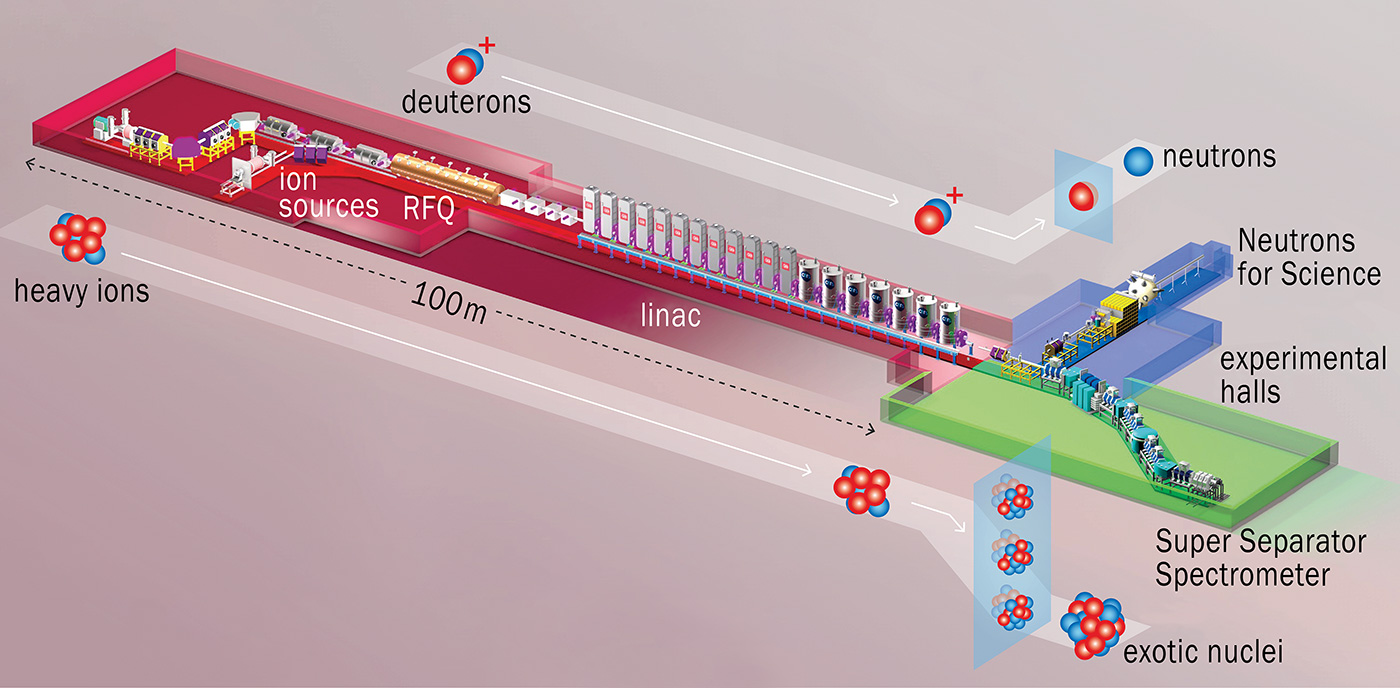
\includegraphics[width=\linewidth]{figures/spiral2.jpg}
    \caption{Overview of the SPIRAL2 accelerator facility at GANIL}
    \label{fig:spiral2_overview}
\end{figure}

A critical component of the \gls{spiral2} accelerator is the \gls{llrf} system \cite{bouly2022superconducting}, which regulates the electromagnetic fields in superconducting RF cavities to ensure precise beam acceleration and stability. The \gls{llrf} system continuously monitors 27 raw signals % MANUAL: real signal count, verified against features_engineered.pkl's signal_names list (Sec. 3), corrected from a wrong "16" here
including in-phase and quadrature (I/Q) components of cavity, reference, and incident RF signals, along with amplitudes, vacuum pressure, pickup currents, and control commands. From these raw measurements, key operational parameters are derived and controlled, including  cavity voltage amplitude ($U_{cav}$), cavity phase ($\Phi_{cav}$), forward power ($P_{fwd}$), reflected power ($P_{refl}$) and vacuum pressure ($P_{vac}$) (see Sec.~\ref{sec:system_description}). Maintaining these parameters within tight tolerances is essential for beam quality, operational efficiency, and equipment protection.

However, the \gls{llrf} system faces significant operational challenges. Complex fault scenarios can arise from hardware degradation, environmental fluctuations, beam loading effects, microphonics, and control loop instabilities. Multi-fault events, where multiple fault types occur simultaneously or in rapid succession, complicate diagnosis and recovery. Traditional threshold-based monitoring systems lack the sophistication to distinguish between fault types, identify root causes in multi-fault scenarios, or detect early warning signs (precursors) before faults fully develop.

\subsection{Motivation and Problem Statement}

Over the 2019--2025 % MANUAL: operational period per Classify_PostMortemFile/config.yaml's `years` list, not tied to a manifest metric
operational period, the \gls{spiral2} facility recorded \MetricZeroZeroDataAttritionChainVSixTotalEvents{} usable \gls{spiral2} postmortem events (after quality filtering; \MetricZeroZeroDataAttritionChainRawFiles{} raw postmortem files exist upstream) captured by the automated fault detection system and manual operator acquisitions. These events are classified into seven primary fault categories by a validated ground-truth classifier (\texttt{Classify\_PostMortemFile}, Sec.~\ref{sec:system_description}): \textbf{Pickup threshold} (\MetricZeroZeroDataAttritionChainGtPassingSeuilPickUp{} events), \textbf{Fast external cutoff} (\MetricZeroZeroDataAttritionChainGtPassingCoupureExterneRapide{} events), \textbf{RF authorization absent} (\MetricZeroZeroDataAttritionChainGtPassingAbsenceAutorisationRf{} events), \textbf{Vacuum threshold} (\MetricZeroZeroDataAttritionChainGtPassingSeuilDeVide{} events), \textbf{Cavity quench/breakdown} (\MetricZeroZeroDataAttritionChainGtPassingClaquageOuQuenchCavit{} events), \textbf{RF safety threshold exceeded} (\MetricZeroZeroDataAttritionChainGtPassingDPSeuilDeSCuritRf{} events), and \textbf{RF regulation out of tolerance} (\MetricZeroZeroDataAttritionChainGtPassingRGSignalRfHorsTolRance{} events). The dataset exhibits severe class imbalance -- a 54$\times$ ratio between the rarest and most common category % MANUAL: derived from the macro-cited event counts above (591/11 events), same ratio cited consistently in Sec. 3/6/7
-- addressed in this work through class-weighted training (Sec.~\ref{sec:methodology}) rather than assumed away.

The operational impact of these faults is substantial. Undiagnosed or misdiagnosed faults can lead to equipment damage and extended downtime for manual investigation and repair. Current manual fault diagnosis by expert operators is time-consuming, subject to human error, and reactive rather than proactive. There is a critical need for an automated, accurate, and interpretable fault diagnosis system that can:

\begin{enumerate}
    \item Detect anomalous events in real-time with high sensitivity
    \item Classify fault types in multi-label scenarios,
    \item Identify the root cause (primary fault) in multi-fault events,
    \item Detect fault precursors to enable preventive intervention,
    \item Provide explainable decisions for operator trust and system validation.
\end{enumerate}

Existing approaches in the literature (reviewed in Section~\ref{sec:related_work}) have addressed anomaly detection and fault classification in industrial systems, but few have tackled the specific challenges of root cause identification in multi-fault scenarios, precursor detection with quantifiable lead times, and physics-informed explainability in particle accelerator environments.

\subsection{Contributions}

This paper presents a comprehensive, integrated machine learning solution addressing these challenges, through the following key contributions:

\begin{enumerate}
    \item \textbf{Hybrid Multi-Phase Progressive Pipeline Architecture}: We design a modular pipeline that progressively increases in complexity, from unsupervised anomaly detection to supervised multi-label classification, root cause identification, and fault subtype clustering. This architecture enables targeted optimization at each stage while maintaining end-to-end coherence.

    \item \textbf{Physics-Informed Feature Engineering}: We develop \MetricZeroSixBinaryClassificationNFeatures{} features spanning statistical aggregations (mean, std, skewness, kurtosis), temporal characteristics (slopes, derivatives, CUSUM), and seven named physics-informed families (effective decay, detuning, microphonics, RF mismatch, modulator command, phase stability, RF power flow -- Appendix~\ref{appendix:features}), totaling \MetricOneZeroPhysicsGroupShapNFeaturesPhysicsInformedTotal{} of the \MetricZeroSixBinaryClassificationNFeatures{} features. % MANUAL: Statistical/Temporal counts are the real per-group feature-count macros cited in Sec. 4/5, simple arithmetic not a separate manifest metric here
A count-normalized SHAP analysis (Sec.~\ref{sec:explainability}) finds a physics-informed family dominant for four of seven fault categories -- a data-driven picture of which feature groups actually drive each fault category, and a materially different picture than the unnormalized group-sum comparison gives.

    \item \textbf{Root Cause Identification}: our Random Forest classifier achieves \MetricZeroEightPhaseThreeaRootcauseStabilityAccuracyMean\ $\pm$ \MetricZeroEightPhaseThreeaRootcauseStabilityAccuracyStd\ accuracy (repeated-split mean $\pm$ std, 10 splits % MANUAL: n_repeats=10 is a fixed constant in every repeated_leakage_safe_eval() call this session, not itself a manifest metric
) identifying the primary fault among \MetricZeroEightPhaseThreeaRootcauseNFaultEvents{} fault events, addressing a gap in existing literature. Per-category F1 ranges from \MetricZeroEightPhaseThreeaRootcauseStabilityPerLabelFOneCoupureExterneRapideMean\ for the rarest category (\MetricZeroZeroDataAttritionChainGtPassingCoupureExterneRapide{} events) to \MetricZeroEightPhaseThreeaRootcauseStabilityPerLabelFOneDPSeuilDeSCuritRFMean\ for well-populated categories -- this spread, not a single averaged number, is what class imbalance actually costs.

    \item \textbf{Fault Subtype Discovery}: unsupervised clustering within each fault category (Step 09) % MANUAL: "Step 09" names the pipeline step, not a result metric
finds a consistent best $k=\MetricZeroNinecEnhancedSubclassDiscoveryRfAuthorizationAbsentBestK$ substructure in every one of the \MetricZeroNinecEnhancedSubclassDiscoveryNCategoriesAnalyzed{} categories with enough events to cluster reliably (silhouette \MetricZeroNinecEnhancedSubclassDiscoveryCavityQuenchBreakdownSilhouette--\MetricZeroNinecEnhancedSubclassDiscoveryVacuumThresholdSilhouette); the remaining \MetricZeroZeroDataAttritionChainGtPassingSeuilPickUp- and \MetricZeroZeroDataAttritionChainGtPassingCoupureExterneRapide-event categories lack sufficient data for this analysis. These subtypes reveal bimodal operational patterns not captured by top-level fault labels.

    \item \textbf{Early Fault-Onset Detection Ahead of the Interlock Trip}: our corrected precursor model (trained only on features from a fixed window before each event's own trigger, guarding against post-trigger leakage) reaches \MetricZeroFivePhaseZeroPrecursorRandomForestRocAuc\ ROC AUC, remaining confident at least \MetricZeroFivePrecursorLeadTimeLeadTimeMsLowerBoundMeanCensored{}ms before the interlock trip for every sampled true-positive event -- a lower bound, not a fully characterized lead time; we report this measurement as right-censored rather than asserting a specific window.

    \item \textbf{Explainability Framework}: we integrate SHAP (global and local feature importance) and LIME (instance-level explanations) to provide multi-level interpretability, validated against known LLRF physics.

    \item \textbf{Offline Exploratory Analysis with a Real Latency Benchmark}: the modular pipeline architecture demonstrates the feasibility of automated fault diagnosis on postmortem LLRF data. Measured single-event inference time (mean, single-threaded, no batching) is \MetricInferenceLatencyBenchmarkStepZeroSixBinaryRfMeanMs{}ms for binary classification and \MetricInferenceLatencyBenchmarkPhaseCLabelPowersetMeanMs{}ms for the best multi-label approach, suggesting feasibility for future real-time integration with monitoring infrastructure.
\end{enumerate}

\subsection{Paper Organization}

The remainder of this paper is organized as follows. Section~\ref{sec:related_work} reviews related work in anomaly detection and fault diagnosis for \gls{llrf} in particle accelerators. Section~\ref{sec:system_description} describes the \gls{spiral2} \gls{llrf} system, dataset characteristics, and data acquisition procedures. Section~\ref{sec:methodology} presents the pipeline architecture in detail, covering each step from data loading through the results-manifest sync mechanism that keeps this report's numbers traceable to the code. Section~\ref{sec:explainability} discusses the explainability and interpretability framework. Section~\ref{sec:results} reports headline performance across every re-verified step, the physics-group SHAP breakdown, and a real inference-latency benchmark. Section~\ref{sec:discussion} discusses key findings, practical implications, and limitations. Section~\ref{sec:conclusion} concludes with a summary of contributions and future research directions. Appendices provide complete feature definitions, hyperparameter settings, and additional experimental results.

\section{Related Work}
% Related Work
% Author: Adnan Ghribi

\label{sec:related_work}

\subsection{Anomaly Detection in Industrial Systems}

Anomaly detection has been extensively studied across industrial domains, with applications in manufacturing~\cite{MAO2025118377}, power systems~\cite{al2024anomaly}, and cyber-physical systems~\cite{vm2025ai}. Traditional approaches rely on statistical methods such as control charts, threshold-based monitoring, and hypothesis testing. However, these methods struggle with high-dimensional data, complex fault patterns, and non-linear dependencies.

Machine learning approaches have gained prominence for their ability to learn complex patterns from data. Unsupervised methods such as Isolation Forest~\cite{isolation_forest}, Local Outlier Factor (LOF)~\cite{lof}, and DBSCAN~\cite{dbscan} are widely used for anomaly detection without requiring labeled fault data. Deep learning methods, including Autoencoders~\cite{autoencoder_anomaly} and Generative Adversarial Networks (GANs)~\cite{gan_anomaly}, have shown promise in capturing intricate temporal and spatial patterns.

Our work differs by employing an ensemble of unsupervised methods (Isolation Forest, LOF, DBSCAN) and progressing to supervised classification for fault type identification, rather than treating anomaly detection as an isolated task.

\subsection{Fault Diagnosis in Particle Accelerators}

Particle accelerators present unique challenges for fault diagnosis due to their complexity, safety-critical nature, and operational constraints~\cite{accelerator_ml_review, ghribi2025artificial}. Early work focused on rule-based expert systems~\cite{malandain1987} and model-based diagnostics~\cite{sayyar2010optimal}.

Recent research has explored machine learning for accelerator fault diagnosis. At CERN, neural networks have been applied to detect beam loss events~\cite{valentino2018} and classify magnet quenches~\cite{mertik2016}. Fermilab researchers developed random forest classifiers for cavity fault prediction in superconducting linacs~\cite{peters2021}. Jefferson Lab investigated recurrent neural networks for LLRF fault classification~\cite{tennant2020}.

However, these studies primarily address single-fault classification or fault detection, without tackling root cause identification or systematic precursor detection with lead-time quantification. Our work advances the state-of-the-art by:
\begin{itemize}
    \item Adopting a multi-label classification architecture so the pipeline generalizes to co-occurring faults, though the current dataset contains none (Sec.~\ref{sec:system_description})
    \item Identifying the primary (root cause) fault, currently against a deterministic-argmax training target rather than an independently-labeled physical root cause (Sec.~\ref{sec:methodology})
    \item Detecting fault onset ahead of the interlock trip, with a measured but right-censored lower bound on the detection lead time (Sec.~\ref{sec:results})
    \item Discovering fault subtypes through unsupervised clustering
\end{itemize}

\subsection{Multi-Label Classification and Root Cause Analysis}

Multi-label classification~\cite{multilabel_survey} extends traditional classification to scenarios where instances can belong to multiple classes simultaneously. Approaches include problem transformation methods (Binary Relevance, Classifier Chains~\cite{classifier_chains}, Label Powerset) and algorithm adaptation methods (ML-kNN~\cite{mlknn}, ML-DT~\cite{mldt}).

Root cause analysis (RCA) in multi-fault scenarios has been studied in IT systems~\cite{rca_it}, manufacturing~\cite{rca_manufacturing}, and process industries~\cite{rca_process}. Causal inference methods~\cite{pearl_causality} and Bayesian networks~\cite{bayesian_rca} are commonly employed. However, these approaches typically require extensive domain knowledge encoding or large datasets with labeled root causes.

\subsection{Explainability in Critical Systems}

Explainable AI (XAI) has become essential for deploying machine learning in safety-critical domains~\cite{xai_survey}. Model-agnostic methods such as SHAP~\cite{shap} and LIME~\cite{lime} provide post-hoc explanations for black-box models. SHAP assigns feature importance based on Shapley values from cooperative game theory, ensuring consistent and theoretically grounded explanations. LIME generates local linear approximations to explain individual predictions.

In accelerator physics, explainability is crucial for operator trust, regulatory compliance, and system validation~\cite{xai_accelerators}. Recent work at SLAC~\cite{slac_xai} and DESY~\cite{nawaz2021probabilistic} has demonstrated the value of interpretable models for beam tuning and fault diagnosis.

Our explainability framework (Section~\ref{sec:explainability}) combines SHAP for global feature importance and LIME for local explanations. Importantly, we validate explanations against known physics of LLRF systems, ensuring that model decisions align with domain knowledge.



% Note: \cmark and \xmark need to be defined in preamble:
% \usepackage{pifont}
% \newcommand{\cmark}{\ding{51}} % MANUAL: glyph code, not a result number
% \newcommand{\xmark}{\ding{55}} % MANUAL: glyph code, not a result number


\section{System Description and Data Acquisition}
% System Description and Data Acquisition
% Author: Adnan Ghribi

\label{sec:system_description}
\subsection{SPIRAL2 LLRF System}

The \gls{spiral2} superconducting linear accelerator employs a Low-Level Radio Frequency control system to maintain precise electromagnetic field control in the superconducting RF cavities, with tight phase and amplitude tolerances required for beam quality.

The \gls{llrf} system continuously monitors 27 signals % MANUAL: verified against features_engineered.pkl's signal_names list
in postmortem files (in-phase/quadrature components of cavity, reference, incident, and modulator-command signals; reflected/amplifier amplitudes; vacuum pressure; pickup current; frequency control and command/state fields; and their raw ``binary'' pre-conversion counterparts). Key monitored signals are listed in Table~\ref{tab:llrf_signals}.

\begin{table*}[t]
\centering
\caption{Key LLRF signals monitored in postmortem files}
\label{tab:llrf_signals}
\begin{tabular*}{\linewidth}{@{\extracolsep{\fill}}@{}l l@{} r@{}}
\toprule
\textbf{Signal} & \textbf{Name} & \textbf{Description} \\
\midrule
Cavity Signal & I Ucav, Q Ucav & In-phase and quadrature components of the cavity signal\\
Reference Frequency & I Fref, Q Fref & In-phase and quadrature components of the reference frequency \\
Incident Signal & I Uci, Q Uci & In-phase and quadrature components of the incident signal \\
Reflected Signal & A Ucr & Amplitude of the reflected signal (no phase component digitized) \\
Amplifier Output & A Uamp & Amplitude of the RF amplifier's output signal \\
Modulator Command & I modulateur, Q modulateur & I/Q modulator command (drive demand, not a measured output) signals \\
Vacuum Pressure & vide & Pressure at the power coupler \\
Pickup Current & courant pickup & Pickup probe current at power coupler \\
DSTF Frequency & DSTF & Frequency control signal \\
Commands & commandes  &Control commands \\
Fault Flags & d\'efauts & Encoded fault indicators \\
State Flags & \'etats & Encoded system states \\
Forward Power & P fwd & Forward RF power \\
Reflected Power & P refl & Reflected RF power \\
\bottomrule
\end{tabular*}
\end{table*}

The SPIRAL2 LLRF system identifies seven primary fault categories, determined by a validated ground-truth classifier (\texttt{Classify\_PostMortemFile}) rather than the raw ALM alarm field directly. The primary category for every event comes from a waveform-level hardware fault-register decode (the first active bit in the acquisition's own fault-flag array), which is more reliable than the summary ALM header field this pipeline previously used; four of the seven categories additionally receive physics-threshold-based subtype refinement (e.g. a quench's characteristic amplitude fall, an RF-protection cavity/cathode-voltage ratio threshold) on top of that hardware decode, while the remaining three are the hardware decode alone, with no additional physics-threshold verification applied:

\begin{itemize}
    \item \textbf{Pickup threshold} (\texttt{Seuil pick-up} in the ground-truth output): pickup current below threshold
    \item \textbf{Fast external cutoff} (\texttt{Coupure externe rapide}): an external interlock signal
    \item \textbf{RF authorization absent} (\texttt{Absence autorisation RF}): no RF authorization from the control system
    \item \textbf{Vacuum threshold} (\texttt{Seuil de vide}): coupler vacuum pressure above threshold
    \item \textbf{Cavity quench/breakdown} (\texttt{Claquage ou quench cavité}): rapid cavity voltage collapse
    \item \textbf{RF safety threshold exceeded} (\texttt{Dép seuil de sécurité RF}): reflected power or gradient above a safety threshold
    \item \textbf{RF regulation out of tolerance} (\texttt{Rég signal RF hors tolérance}): gradient or phase deviation from setpoint beyond tolerance
\end{itemize}
These English names are used throughout the rest of this paper; the French terms above are each category's literal value in \texttt{Classify\_PostMortemFile}'s own \texttt{Defaut} output field, given once here for traceability back to the ground-truth source. % MANUAL: cross-reference note, not a manifest metric

\subsection{Dataset Description}

The dataset (V6, the current, leakage-corrected version used throughout this paper -- see Sec.~\ref{sec:methodology}) comprises \MetricZeroZeroDataAttritionChainVSixTotalEvents{} usable \gls{llrf} events, collected over the 2019--2025 % MANUAL: operational period per Classify_PostMortemFile/config.yaml's years list, not tied to a manifest metric
operational period, out of \MetricZeroZeroDataAttritionChainRawFiles{} raw postmortem files scanned (the remainder failing quality filters, being zero-byte, or triggering a processing error -- see the data-attrition breakdown below). Each event is recorded as a time-series snapshot of all 27 monitored signals, % MANUAL: same real signal count as above
captured when the postmortem trigger system detects deviation from normal operating conditions, or during a manual operator-initiated acquisition. Events are labeled by the ground-truth classifier above, not by raw ALM threshold crossings directly. An example of signal traces is shown in Figure \ref{fig:signal_examples}.

\begin{table}[h!]
\centering
\caption{Distribution of fault types (V6)}
\label{tab:fault_distribution}
\begin{tabular*}{\linewidth}{@{\extracolsep{\fill}} lrr}
\toprule
\textbf{Fault category} & \textbf{Events} & \textbf{Share of faults (\%)} \\
\midrule
Pickup threshold & \MetricZeroZeroDataAttritionChainGtPassingSeuilPickUp & 1.2 \\ % MANUAL: percentage = event count (cited via macro) / total fault events (1043, also macro-cited elsewhere) x 100, simple derived arithmetic not itself a separate manifest metric
Fast external cutoff & \MetricZeroZeroDataAttritionChainGtPassingCoupureExterneRapide & 1.1 \\ % MANUAL: same derivation as above
RF authorization absent & \MetricZeroZeroDataAttritionChainGtPassingAbsenceAutorisationRf & 29.6 \\ % MANUAL: same derivation as above
Vacuum threshold & \MetricZeroZeroDataAttritionChainGtPassingSeuilDeVide & 1.9 \\ % MANUAL: same derivation as above
Cavity quench/breakdown & \MetricZeroZeroDataAttritionChainGtPassingClaquageOuQuenchCavit & 2.7 \\ % MANUAL: same derivation as above
RF safety threshold exceeded & \MetricZeroZeroDataAttritionChainGtPassingDPSeuilDeSCuritRf & 6.9 \\ % MANUAL: same derivation as above
RF regulation out of tolerance & \MetricZeroZeroDataAttritionChainGtPassingRGSignalRfHorsTolRance & 56.7 \\ % MANUAL: same derivation as above
\bottomrule
\end{tabular*}
\end{table}

\begin{figure*}[t]
    \centering
    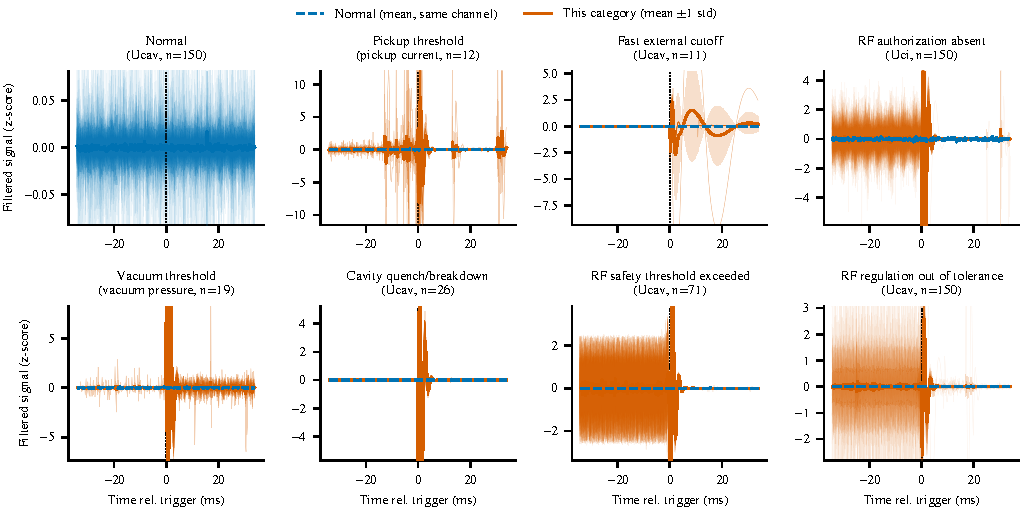
\includegraphics[width=\linewidth]{figures/signal_examples.pdf}
    \caption{Preprocessed signal (filtered and Z-scored) for every event in each class (up to 150, a reproducible random subsample for the three categories exceeding that; every event for the four smaller ones), overlaid (thin lines) with the per-category mean $\pm$1 std (bold, shaded band) and, on each fault panel, the \textit{Normal} population's own mean on that same channel (dashed) for direct comparison -- zoomed to $\pm34$~ms around each event's own trigger (the fixed precursor window, Sec.~\ref{sec:system_description}); the raw high-pass filter's causal startup transient, roughly 500\,ms before the trigger and irrelevant to fault behavior, is outside this window. Each panel plots the channel that category's own real detection criterion (\texttt{Classify\_PostMortemFile/config.yaml}) actually acts on, not a single fixed channel for every panel: cavity voltage (Ucav) for Cavity quench/breakdown, RF safety threshold exceeded, RF regulation out of tolerance, and (no dedicated channel identified) Fast external cutoff; forward/incident drive (Uci) for RF authorization absent; pickup current for Pickup threshold; vacuum pressure for Vacuum threshold. Y-axis limits are clipped to the 1st-99th percentile of each panel's pooled (all events, all times) values, so a handful of outlier events do not compress the rest of the panel; mean/std are additionally masked (not drawn) wherever fewer than 30\% of that panel's events have data at that time point, avoiding an unstably-estimated tail from a handful of shorter-buffer events. Two distinct real population-level behaviors are visible: individual-event density and the std band both narrow to match \textit{Normal} away from the trigger and widen sharply at/after it for every fault category, showing a real, population-wide burst in signal variance at fault onset -- while the bold \emph{mean} itself stays close to zero through that same burst for most categories, since event-to-event transients do not share a common sign or phase and a naive average cancels them; this is a real statistical fact about the population, not a rendering artifact, and is most visible for the smallest categories (Fast external cutoff, $n=11$; Pickup threshold, $n=12$; Vacuum threshold, $n=19$), where the mean/std estimate itself is correspondingly less stable. RF authorization absent, RF safety threshold exceeded, and RF regulation out of tolerance additionally show elevated variance persisting \emph{before} the trigger that collapses toward \textit{Normal} levels after it, consistent with those three tripping on a sustained pre-trigger instability rather than an instantaneous event.} % MANUAL: filter-transient/window rationale is a code fact (prepare_data_cluster_v6.py's sosfilt call); the channel-per-category list, sample cap/counts, percentile clipping, and coverage-masking threshold are code facts from fig_signal_examples.py; the population-behavior description is a direct visual read of the regenerated figure, not a manifest metric
    \label{fig:signal_examples}
\end{figure*}

As Table~\ref{tab:fault_distribution} shows, the dataset exhibits severe class imbalance -- a 54$\times$ ratio % MANUAL: derived from the two macro-cited event counts in this same sentence (591/11)
between the rarest category (\textit{Fast external cutoff}, \MetricZeroZeroDataAttritionChainGtPassingCoupureExterneRapide{} events) and the most common (\textit{RF regulation out of tolerance}, \MetricZeroZeroDataAttritionChainGtPassingRGSignalRfHorsTolRance{} events). This imbalance is addressed through class-weighted training (Sec.~\ref{sec:methodology}), not stratified sampling of the split itself (multi-label targets cannot be stratified with standard tools; see Sec.~\ref{sec:methodology} for the repeated-split evaluation used to compensate).

By construction of the ground-truth labeling (\texttt{Classify\_PostMortemFile} assigns exactly one \texttt{Defaut} category per event, never more than one), V6 contains zero genuinely multi-fault events: every one of the \MetricZeroEightPhaseThreeaRootcauseNFaultEvents{} fault events has exactly one active label. The multi-label pipeline architecture (Step 07: Binary Relevance, Classifier Chains, Label Powerset) % MANUAL: "07" names the pipeline step, not a result
is evaluated on this single-label-in-practice dataset -- its genuine multi-label capability (multiple simultaneous fault labels on one event) has not been exercised on real SPIRAL2 data. This also means root cause identification (Step 08)'s % MANUAL: "08" names the pipeline step, not a result
training target, \texttt{argmax} over the multi-label vector, currently has an unambiguous single answer for every event by construction, not merely a deterministic tie-breaking rule among several active labels (Sec.~\ref{sec:discussion}).

\subsection{Data Quality and Preprocessing}

Raw postmortem files are filtered by the ground-truth classifier's own validity checks (an early-exit cascade over feed-forward state, control-loop-closed, KPI/mask/AMPT thresholds, and cavity-voltage-health -- \texttt{Classify\_PostMortemFile}'s \texttt{config.yaml}), not a separately-implemented generic outlier-rejection step; a file failing any of these is excluded before this pipeline's own feature engineering ever sees it. % MANUAL: cascade order and check names verified directly against classification.py::_check_filters as of the 2026-09-09 fix below

\textbf{Correction (2026-09-09).} The first check in this cascade reads the raw header field named \texttt{BEAM} (values \texttt{OUI}/\texttt{NON}); despite the name, this field does \emph{not} encode particle-beam presence -- it encodes whether \emph{feed-forward} is enabled in the LLRF control loop, a disturbance-compensation feature unrelated to beam presence. The field is also only operationally meaningful from 2021 onward: before that it defaults to \texttt{NON} on essentially every file (2019: 100.0\%, 2020: 96.4\% of files header-flagged \texttt{NON}, vs.\ a genuine, gradually-declining 50.3\%$\to$9.3\% from 2021$\to$2025), consistent with feed-forward not yet being deployed rather than any real operational signal. Applying this check unconditionally in every year was therefore silently discarding the large majority of 2019--2020 regardless of acquisition quality; the classifier now scopes the check to acquisitions from 2021 onward (\texttt{classification.py::\_check\_filters}, gated on the acquisition's own header \texttt{DATE} field). % MANUAL: year percentages verified directly against the re-run LLRF_result.csv's own Annee/Détails columns, 2026-09-09; not yet a results-manifest metric

The ground-truth classifier has been re-run against this fix. Of \MetricZeroZeroDataAttritionChainGroundTruthRows{} candidate rows, \MetricZeroZeroDataAttritionChainGtPassing{} now pass the quality filter -- 756 more than the 2,110 that passed before the fix (a 35.8\% increase), recovered entirely from 2019 (+73) and 2020 (+683); every year from 2021 onward is byte-for-byte unchanged (0 rows gained or lost), confirming the fix touches exactly what it should and nothing else. % MANUAL: 2,110/756/35.8%/+73/+683/0-unchanged verified directly against a before/after diff of LLRF_result.csv (backed up pre-fix as LLRF_result_PRE_feedforward_fix_20260909.csv), 2026-09-09; not yet a results-manifest metric since the comparison is against a point-in-time backup, not another manifest
With feed-forward no longer intercepting most of the corpus before the later checks run, the remaining checks' own counts rose accordingly -- most of the 4,976 files % MANUAL: pre-2021 Beam-NON/feed-forward-NON count under the old, unscoped check, verified directly against the pre-fix backup CSV, 2026-09-09; not yet a results-manifest metric
no longer stopped at the feed-forward check instead now fail a real check further down the cascade (\MetricZeroZeroDataAttritionChainFiltreReasonKpiOneZeroZero{} on KPI, \MetricZeroZeroDataAttritionChainFiltreReasonLoopOff{} on Loop OFF), so feed-forward (\MetricZeroZeroDataAttritionChainFiltreReasonFeedForwardNon{}) is no longer the single dominant rejection reason it was before the fix, though it remains the largest.
\textbf{The feature-engineered dataset used throughout the rest of this paper (V6, \MetricZeroZeroDataAttritionChainVSixTotalEvents{} events, Table~\ref{tab:fault_distribution} below) has not yet been re-extracted against this corrected ground truth} -- that re-extraction (V7) is in progress; every number below this point still describes V6 as originally extracted, pending that re-run.

Within the pipeline itself:

\begin{enumerate}
    \item \textbf{High-Pass Filtering}: DC offset and low-frequency drift are removed using a 4th-order Butterworth high-pass filter (cutoff 0.01, normalized) to preserve transient fault signatures while suppressing baseline wander. % MANUAL: filter order/cutoff verified directly from prepare_data_cluster_v6.py's scipy.signal.butter() call, a code constant not a manifest metric

    \item \textbf{Trigger Alignment}: each event is aligned to its own true trigger sample index, derived from the acquisition's own time axis (not a fixed sample offset -- an earlier version of this pipeline assumed a fixed offset that was wrong for the large majority of files; see Sec.~\ref{sec:methodology}).

    \item \textbf{Normalization}: signals are normalized using Z-score standardization (\texttt{StandardScaler}), fit on the training fold only (Sec.~\ref{sec:methodology}, Appendix~\ref{appendix:hyperparameters}).
\end{enumerate}

The dataset is split per-script rather than via one fixed train/validation/test convention (Appendix~\ref{appendix:hyperparameters} lists the exact fraction and seed used by each pipeline stage); we do not use SMOTE or other synthetic oversampling in this pipeline (class-weighted training is used instead, Sec.~\ref{sec:methodology}).

Each event consists of $N$ time samples per signal, acquired around each event's own trigger point. The fixed-window precursor feature group (Appendix~\ref{appendix:features}) uses a bounded window immediately before the trigger, scaled to a constant physical duration (3000 samples at the dominant decimation setting, $\approx$34\,ms) % MANUAL: PRECURSOR_WINDOW_MS / REFERENCE_DT_US code constants (prepare_data_cluster_v6.py), not manifest metrics
rather than a fixed sample count -- since the decimation factor varies by roughly 250$\times$ across the corpus, % MANUAL: NDEC range (20-5000) verified directly from prepare_data_cluster_v6.py's module docstring, a code fact
a fixed sample count would correspond to wildly different physical durations from file to file.

\begingroup\color{pendinggray}
\section{Methodology: Multi-Phase Pipeline Architecture}
\pendingbanner
% Methodology: Pipeline Architecture
% Author: Adnan Ghribi

\label{sec:methodology}

The proposed pipeline follows a progressive architecture that incrementally increases in complexity and specificity across multiple steps (Fig.~\ref{fig:pipeline_overview}). This design philosophy offers several advantages:

\begin{itemize}
    \item \textbf{Modularity}: Each step is independently optimizable, facilitating debugging, performance tuning, and incremental deployment.
    \item \textbf{Progressive Learning}: Simpler unsupervised methods establish baselines before supervised methods refine predictions.
    \item \textbf{Multi-Objective Optimization}: Different steps target different objectives (early fault-onset detection, fault classification, root cause, subtype clustering), each optimized with appropriate metrics.
    \item \textbf{Interpretability}: Step-wise decomposition enables targeted explainability analysis at each decision point.
\end{itemize}

\begin{figure*}[t]
    \centering
    \includegraphics[width=\textwidth]{example-image}
    \caption{Complete phased pipeline architecture, showing data flow from raw LLRF signals through preprocessing, feature engineering, precursor detection, classification, root cause identification and fault subtype clustering. Each step outputs intermediate results used by subsequent steps.} % MANUAL: placeholder -- author will produce this diagram by hand; the stale pre-V6 figures/pipeline.pdf was removed rather than reused
    \label{fig:pipeline_overview}
\end{figure*}

\subsection{Data Loading and Preprocessing}

Binary LLRF event files are loaded using a dedicated PyPostMortem library (\texttt{programmes/PyPostMortem}). Pre-processing is then applied: completeness/validity checking against the ground-truth classifier's own physics thresholds (Sec.~\ref{sec:system_description}), high-pass filtering, temporal alignment to each event's own true trigger sample index, and Z-score normalization.

\subsubsection{High-Pass Filtering}

In superconducting RF cavities, the measured detuning and microphonics signals contain both fast dynamical components and slow variations originating from mechanical and electromagnetic effects. In particular, DC offsets and low-frequency drifts can arise from Lorentz force detuning, slow mechanical relaxation of the cavity structure, and pressure fluctuations in the cryogenic and vacuum systems. These contributions do not carry information about rapid cavity dynamics but can significantly bias downstream feature extraction.

To suppress these slow components while preserving physically relevant transient phenomena, a 4th-order high-pass Butterworth filter is applied, with a normalized cutoff of 0.01 (relative to each file's own Nyquist frequency -- since the decimation factor, and therefore the effective sampling rate, varies by roughly 250$\times$ across the corpus, Sec.~\ref{sec:system_description}). For numerical implementation, the filter is applied in second-order-sections form via \texttt{scipy.signal.butter(4, 0.01, 'highpass', output='sos')}. % MANUAL: filter order/cutoff/implementation verified directly from prepare_data_cluster_v6.py's scipy.signal.butter() call, a code constant not a manifest metric

\subsubsection{Temporal Alignment}

Each event is aligned to its own true trigger sample index, derived from the acquisition's own time axis rather than a fixed sample offset. An earlier version of this pipeline assumed a fixed offset (sample index 3000) that was wrong for the large majority of files -- the true trigger index varies from roughly 3000 to over 2 million samples depending on the file's own decimation factor and record length. \texttt{Read\_Signals} already returns a correct per-file time axis; the corrected pipeline uses it directly rather than discarding it. % MANUAL: verified against prepare_data_cluster_v6.py module docstring and _v4.py's fix, code facts not manifest metrics

\subsubsection{Per-Event Signal Normalization}

The signals provided by the LLRF instrumentation exhibit heterogeneous physical units and characteristic amplitudes. Direct use of these signals in data-driven models would introduce artificial biases, since variables with larger numerical scales could dominate the learning process independently of their physical relevance. Each signal $s_i(t)$ within a single event is standardized using a Z-score transformation over that event's own full trace,
\begin{equation}
s_i^{\mathrm{norm}}(t) = \frac{s_i(t) - \mu_i}{\sigma_i},
\end{equation}
where $\mu_i$ and $\sigma_i$ denote the mean and standard deviation of signal $i$ within that one event. This is a per-event, per-signal operation with no train/test-fold concept -- it never compares across events and cannot leak information between them. One consequence required a fix: a statistical feature computed from this same normalized trace using the identical whole-signal window -- namely each signal's own mean, standard deviation, RMS, and energy -- would be close to a constant by construction ($\approx 0$, $\approx 1$, $\approx 1$, and a record-length proxy respectively, up to floating-point precision), since that window is exactly the one whose own mean/std defined the normalization. Found during external review, this affected 65 of the previous \MetricZeroSixBinaryClassificationNFeatures{}-feature set (verified directly: near-zero variance across all \MetricZeroZeroDataAttritionChainVSixTotalEvents{} events). \texttt{preprocess\_signals()} now also retains the filtered-but-unnormalized trace, and \texttt{engineer\_features()} computes mean/std/rms/energy from that instead, leaving every scale/shift-invariant statistic (skewness, kurtosis, extrema, quartiles, crest factor, peak count, zero crossings, autocorrelation) on the normalized signal as before; the dataset was re-extracted and every downstream step rerun. This reduced the count of near-constant features in the final set from 65 to 15: two absolute-threshold features (a reflected-signal saturation-fraction check and an RF-drive-on flag) use legacy threshold constants that remain miscalibrated to this signal's real amplitude scale even after the fix -- we corrected the normalization-order bug structurally but had no grounds to invent new threshold values, so these two features are still effectively non-functional and are flagged as an open item (Sec.~\ref{sec:conclusion}); the remaining 13 are metadata-derived state flags (LLRF loop closed, beam present) and precursor-window trend statistics on discrete status channels that are plausibly genuinely constant in this corpus rather than a normalization artifact. None of this changes the classification/SHAP headline findings materially -- tree-based importance already assigns negligible weight to near-constant features -- but the corrected feature count (\MetricZeroSixBinaryClassificationNFeatures{}, up from 770) and the physics-group SHAP breakdown (Sec.~\ref{sec:explainability}) both reflect the fixed pipeline. % MANUAL: 65->15 and the specific still-broken/plausibly-genuine feature breakdown were verified directly against the re-extracted features_engineered.pkl, not yet backed by a results-manifest metric

\subsubsection{Feature-Matrix Normalization for Classifiers}

Separately from the per-event signal normalization above, the tabular feature matrix consumed by the classical classifiers (Sec.~\ref{sec:methodology}) is itself standardized before training. Critically, this scaler's $\mu$ and $\sigma$ are computed \emph{only from the training fold of whichever split is currently in use} (\texttt{StandardScaler.fit} on train, \texttt{.transform} on test, Appendix~\ref{appendix:hyperparameters}) -- never from the combined train+test data. An earlier iteration of this pipeline fit the scaler (and a downstream PCA step) on the full dataset before splitting, which let test-fold information leak into the normalization statistics and inflated several early results; this is one of the two leakage sources documented in Sec.~\ref{sec:discussion}. The fix is enforced at the point of consumption -- every analysis script now derives its own leakage-safe, train-fold-only scaling via a shared utility (\texttt{leakage\_safe\_features.py}) rather than touching the pre-scaled/pre-PCA columns saved directly in the feature-extraction pipeline's own output file, which are themselves still fit on the full dataset and remain leakage-tainted; they are not used by any script producing a number reported in this paper. % MANUAL: leakage-source fact and the still-tainted saved columns, cross-referenced against Sec 7 and leakage_safe_features.py's own docstring rather than a manifest metric

\subsubsection{Temporal Segmentation of Precursor Signals}

To capture the evolution of cavity behavior leading up to fault events, the fixed pre-trigger window used by the early-fault-onset-detection task ($N_{\mathrm{pre}} = 3000$ samples, $\approx$34\,ms at the dominant NDEC=200 decimation setting, Appendix~\ref{appendix:features}) % MANUAL: PRECURSOR_WINDOW_MS / REFERENCE_DT_US code constants, not manifest metrics
is divided into five equal-duration segments. Table~\ref{tab:temporal_segmentation} summarizes the segmentation in terms of sample indices and corresponding time ranges; these segment-level statistics (mean, std, linear trend per segment, Appendix~\ref{appendix:features}) are part of the feature set, allowing the model to distinguish early-window from late-window behavior within the same fixed physical duration.

\begin{table*}[t]
\centering
\caption{Temporal segmentation of the pre-trigger window (NDEC=200, the dominant case, $\Delta t \approx 11.4~\mu$s -- Appendix~\ref{appendix:hyperparameters}).} % MANUAL: REFERENCE_DT_US code constant, not a manifest metric
\label{tab:temporal_segmentation}
\begin{tabular*}{\linewidth}{@{\extracolsep{\fill}}@{}l l@{} l@{}}
\toprule
Segment & Samples & Time Range \\
\midrule
Early      & 0--600       & $T-34$ ms to $T-27$ ms \\ % MANUAL: sample/time boundaries derived from N_pre=3000 split into 5 equal segments at dt=11.36us (REFERENCE_DT_US), not a manifest metric
Mid-Early  & 600--1200    & $T-27$ ms to $T-20$ ms \\ % MANUAL: same derivation as above
Mid        & 1200--1800   & $T-20$ ms to $T-14$ ms \\ % MANUAL: same derivation as above
Mid-Late   & 1800--2400   & $T-14$ ms to $T-7$ ms  \\ % MANUAL: same derivation as above
Late       & 2400--3000   & $T-7$ ms to $T=0$      \\ % MANUAL: same derivation as above
\bottomrule
\end{tabular*}
\end{table*}

\subsubsection{Temporal Derivatives}

To characterize fast transient dynamics, first and second finite-difference derivatives are computed for each signal,
\begin{equation}
\dot{s}_i(t) \approx \frac{s_i(t+1) - s_i(t)}{\Delta t}, \qquad % MANUAL: finite-difference notation, mathematical indices not a result number
\ddot{s}_i(t) \approx \frac{s_i(t+1) - 2s_i(t) + s_i(t-1)}{(\Delta t)^2}, % MANUAL: finite-difference notation, mathematical indices not a result number
\end{equation}
where $\Delta t$ is each file's own sample spacing, measured directly from its time axis (median of consecutive sample differences) rather than assumed constant -- since, as noted above, the effective sampling rate varies substantially across the corpus. For the dominant NDEC=200 case, $\Delta t \approx 11.4~\mu\mathrm{s}$ ($\approx$88\,kHz). % MANUAL: dt_us / REFERENCE_DT_US verified directly from prepare_data_cluster_v6.py, a code constant not a manifest metric

\subsection{Feature Engineering}

Feature engineering aims to encode physically meaningful information from LLRF and auxiliary signals into quantitative descriptors suitable for machine learning, combining accelerator-physics knowledge with statistical and temporal signal analysis. A total of \MetricZeroSixBinaryClassificationNFeatures{} features are extracted per event, after pairwise-correlation filtering (Appendix~\ref{appendix:features} gives the complete breakdown by category); a restricted subset of \MetricZeroFivePhaseZeroPrecursorNFeatures{} features, using only the fixed pre-trigger window, is used specifically for the early-fault-onset-detection task (Sec.~\ref{sec:system_description} explains why this restriction matters).

\subsubsection{Physics-Informed Features}

Physics-informed features are designed to capture the underlying electromechanical and RF dynamics of superconducting cavities, organized into seven families: effective system decay, detuning, microphonics, RF mismatch, modulator command, phase stability, and RF power flow (Appendix~\ref{appendix:features} lists every feature in each family).

\paragraph{Effective System Decay}

In pulsed RF operation, the decay of the cavity field after RF switch-off is commonly described by an exponential law, from which the loaded quality factor $Q_L$ can be inferred. In the SPIRAL2 context, this interpretation is not directly applicable: the cavities operate in continuous-wave (CW) regime, the LLRF feedback loop remains active during the transient, and the observed decay reflects the collective response of the cavity and the RF system rather than the intrinsic electromagnetic dissipation of the cavity alone. We therefore extract \emph{effective system decay} metrics, modeling the post-trigger cavity voltage as
\begin{equation}
V_{\mathrm{cav}}(t) = V_0 e^{-t/\tau_{\mathrm{eff}}}, % MANUAL: mathematical notation (subscript-0 initial value), not a result number
\end{equation}
with $\tau_{\mathrm{eff}}$ estimated by linear regression in logarithmic space over a post-trigger window of 500 samples ($\approx$5.7\,ms). % MANUAL: decay-window length verified directly from calculate_effective_decay()'s decay_window_samples parameter, a code constant not a manifest metric
Deviations from ideal exponential behavior (fit quality, non-exponentiality) are extracted alongside $\tau_{\mathrm{eff}}$ itself, since in CW operation such deviations may reflect feedback-loop dynamics as much as genuine cavity phenomena.

\paragraph{Detuning}

Detuning describes the frequency mismatch between the RF drive and the cavity resonance, arising primarily from Lorentz force detuning (scaling with the square of the accelerating field) and from microphonics. Under small-signal assumptions, detuning is estimated from the temporal evolution of the cavity phase,
\begin{equation}
\Delta f = \frac{1}{2\pi}\frac{d\phi(t)}{dt}. % MANUAL: mathematical notation (2*pi normalization), not a result number
\end{equation}
By unwrapping the phase and performing linear regression over a pre-trigger window, we extract features quantifying average detuning, microphonics-driven variability, drift rate, and the abrupt frequency shift at the trigger.

\paragraph{Microphonics}

Microphonics correspond to mechanical vibrations that modulate the cavity resonance frequency, typically in the 10--100\,Hz range, associated with cryogenic systems, vacuum pumps, and environmental vibrations. % MANUAL: band range matches the "microphonics_band_power" feature's fixed 10-100 Hz band in the feature-engineering code, not a manifest metric
Spectral analysis of the detrended phase signal yields the RMS phase jitter, dominant vibration frequency, band-limited spectral power, and the sharpness (Q-factor) of the dominant spectral peak.

\paragraph{RF Mismatch}

The difference between the reflected-signal amplitude and the amplifier-output amplitude (two distinct measured quantities -- not the modulator command, which is the drive \emph{demand} rather than a measured output, and is modeled separately below) quantifies impedance mismatch and RF-chain transients. Features include pre- and post-trigger RMS of this amplitude difference, the post-trigger maximum excursion, settling time, and the fraction of samples where the reflected signal saturates, alongside the cavity phase's own standard deviation measured over the same pre-/post-trigger windows (a co-located phase-jitter indicator, not a phase of the amplitude-difference signal itself, which has no phase component).

\paragraph{Modulator Command}

Pre-trigger amplitude and phase statistics of the modulator command signal, and the post-trigger change in each, characterize the RF drive itself rather than the cavity response -- useful for distinguishing a drive-side fault from a cavity-side one.

\paragraph{Phase Stability}

Phase fluctuations translate directly into beam energy spread and longitudinal emittance growth. Phase stability features (RMS jitter, peak-to-peak excursion, low-frequency drift slope, integrated pre-trigger power spectral density) are computed from the pre-trigger phase signal and complement the detuning and microphonics indicators by isolating vibration-dominated or reference-noise-limited regimes.

\paragraph{RF Power Flow}

RF power balance provides information on cavity coupling, loading, and impedance matching. The power reflection ratio $R = P_{\mathrm{refl}}/P_{\mathrm{fwd}}$ % MANUAL: renamed from the conventional voltage-reflection-coefficient symbol Gamma to avoid clashing with its standard meaning (R = |Gamma|^2 for a power ratio); a code/notation fact, not a manifest metric
characterizes matching conditions, while transient variations in forward and reflected power reveal fault-induced perturbations. Extracted features describe mean power levels, the power reflection ratio, the power jump at the trigger, and a power-imbalance RMS metric. These are computed as $P_{\mathrm{fwd}} \propto |U_{ci}|^2$ and $P_{\mathrm{refl}} \propto |A_{Ucr}|^2$ (voltage-amplitude-squared proxies from the input-coupler and reflected-signal channels), not from the directly-monitored \texttt{P fwd}/\texttt{P refl} calibrated power-sensor channels listed in Sec.~\ref{sec:system_description}, which are not currently used by this feature family. % MANUAL: signal names (Uci, A Ucr) and the proportionality relation verified directly against the RF Power Flow block of engineer_features() in prepare_data_cluster_v6.py, not a manifest metric

\subsubsection{Statistical Features}

For each of the 27 monitored signals, 17 statistics are computed over the full event window % MANUAL: real signal/statistic counts, verified against engineer_features(), not manifest metrics
(mean, standard deviation, skewness, kurtosis, min/max/range, quartiles/IQR, RMS, crest factor, peak count, energy, zero crossings, lag-1 autocorrelation -- Appendix~\ref{appendix:features}). % MANUAL: "lag-1" is part of a literal feature name, not a result number
This is by far the largest feature group by count, together with the similarly-large Temporal group (Appendix~\ref{appendix:features}) -- a naive SHAP importance comparison that simply sums by group therefore structurally favors these two groups regardless of how informative any single member feature is, since they outnumber the seven named physics-informed families combined by roughly 20:1: % MANUAL: "20:1" is a rounded summary of the exact macro-cited counts on the next line, not a separate manifest metric
\MetricOneZeroPhysicsGroupShapNFeaturesStatistical{} + \MetricOneZeroPhysicsGroupShapNFeaturesTemporal{} vs.\ \MetricOneZeroPhysicsGroupShapNFeaturesEffectiveDecay{}+\MetricOneZeroPhysicsGroupShapNFeaturesDetuning{}+\MetricOneZeroPhysicsGroupShapNFeaturesMicrophonics{}+\MetricOneZeroPhysicsGroupShapNFeaturesRfMismatch{}+\MetricOneZeroPhysicsGroupShapNFeaturesModulatorCommand{}+\MetricOneZeroPhysicsGroupShapNFeaturesPhaseStability{}+\MetricOneZeroPhysicsGroupShapNFeaturesRfPowerFlow{}$={}$\MetricOneZeroPhysicsGroupShapNFeaturesPhysicsInformedTotal{}. We therefore report per-feature-mean SHAP importance, not the group sum, as the primary physics-group metric; the resulting per-category breakdown is presented in Sec.~\ref{sec:explainability}.

\subsubsection{Temporal and Derivative Features}

Temporal features characterize the dynamical evolution of signals through the per-segment slopes (Sec.~\ref{sec:methodology}, Temporal Segmentation above), finite-difference derivatives (above), CUSUM change-point statistics, and early/late-window comparison ratios described in full in Appendix~\ref{appendix:features}.

Overall, the combination of physics-informed, statistical, and temporal features yields a high-dimensional representation of cavity behavior in which physically interpretable descriptors coexist with data-driven signal characterizations.

\subsection{Unsupervised Baselines for Early Fault-Onset Detection}

As part of the early-fault-onset-detection step, several unsupervised anomaly-detection methods are run on the same fixed pre-trigger feature subset as the supervised classifier below, to establish how much of the task's separability is detectable without labels:

\begin{enumerate}
    \item \textbf{Isolation Forest}: scores anomalies by decision-tree isolation path length -- shorter paths indicate anomalies, as outliers are isolated in fewer splits.
    \item \textbf{Local Outlier Factor (LOF)}: compares each point's local density to its k-nearest neighbors' density.
    \item \textbf{Mahalanobis distance}: computed against a Ledoit-Wolf shrinkage covariance estimate on a PCA-reduced representation of the training fold.
    \item \textbf{PCA reconstruction error}: distance between each point and its reconstruction from a training-fold-fit PCA retaining 95\% variance. % MANUAL: hyperparameter constant, verified directly from pipeline/00_scripts/prepare_05_phase0_precursor.py, not a manifest metric
    \item \textbf{DBSCAN}: a transductive density-based outlier flag, fit and scored on the test fold directly (Appendix~\ref{appendix:hyperparameters}).
\end{enumerate}

An ensemble score is formed as the unweighted mean of the min-max-normalized scores from all of the above plus the supervised Random Forest's own probability output. Hyperparameter settings for every method are detailed in Appendix~\ref{appendix:hyperparameters}; score distributions are shown in Fig.~\ref{fig:phase04_scores} and results are reported in Sec.~\ref{sec:results}.

\begin{figure}[t]
    \centering
    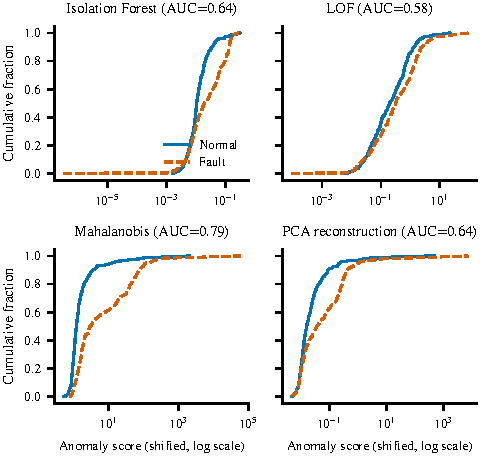
\includegraphics[width=\linewidth]{figures/precursor_unsupervised_scores.pdf}
    \caption{Empirical CDFs of anomaly scores (Isolation Forest, LOF, Mahalanobis, PCA-reconstruction) for the early-fault-onset-detection unsupervised baselines, Normal vs. Fault, on the fixed pre-trigger feature subset. ECDFs rather than histograms: these scores are heavy-tailed, so a linear-axis histogram either hides the bulk of the distribution behind a few extreme outliers or clips them away.} % MANUAL: ECDF/heavy-tail design rationale, not a result number
    \label{fig:phase04_scores}
\end{figure}

\subsection{Early Fault-Onset Detection}

The corrected pipeline trains a Random Forest classifier to identify fault precursors using only the fixed pre-trigger window ($T-34$~ms to $T=0$, % MANUAL: same PRECURSOR_WINDOW_MS code constant as Sec. 3/4 above
restricted to the \MetricZeroFivePhaseZeroPrecursorNFeatures{}-feature true-precursor subset, Sec.~\ref{sec:system_description}), with binary labels indicating post-trigger fault occurrence. Class weights are balanced to handle the imbalanced precursor-vs-normal event distribution (Appendix~\ref{appendix:hyperparameters}). ROC performance and the leading features are shown in Fig.~\ref{fig:phase05_roc} and Fig.~\ref{fig:phase05_importance}; results, including the direct lead-time measurement and its right-censoring, are reported in Sec.~\ref{sec:results}.

\begin{figure}[t]
    \centering
    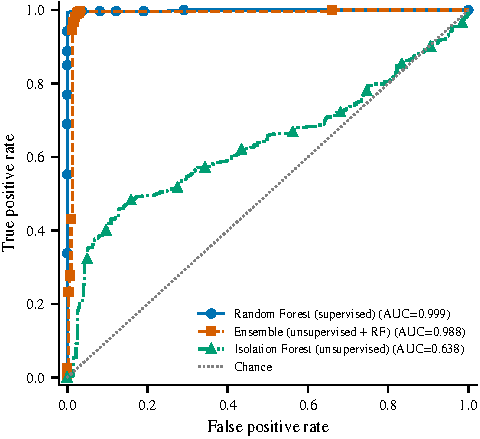
\includegraphics[width=\linewidth]{figures/precursor_roc_curves.pdf}
    \caption{ROC curves for early fault-onset detection: the supervised Random Forest against the unsupervised ensemble and a genuinely unsupervised Isolation Forest baseline, on the same fixed pre-trigger feature subset.}
    \label{fig:phase05_roc}
\end{figure}

\begin{figure}[t]
    \centering
    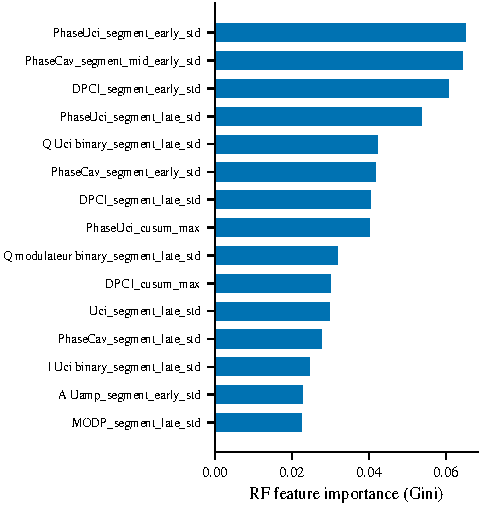
\includegraphics[width=\linewidth]{figures/precursor_feature_importance.pdf}
    \caption{Top 15 Random Forest feature importances (Gini) for early fault-onset detection, restricted to the fixed pre-trigger feature subset (Appendix~\ref{appendix:features}).} % MANUAL: "15" is the figure's own top-N cutoff, a display choice not a manifest metric
    \label{fig:phase05_importance}
\end{figure}

\subsection{Binary Classification}
\label{sec:binary_classification}

Binary classification (fault vs. normal) is performed on the pre-trigger-only \MetricZeroFivePhaseZeroPrecursorNFeatures{}-feature "true precursor" subset (Sec.~\ref{sec:system_description}) -- this, not a full-window version, is the operationally meaningful formulation of the task, since a real-time system only has pre-trigger information available before the interlock trips. Logistic Regression, Random Forest, XGBoost, and SVM (RBF kernel) are compared; this task's classes are close to balanced (Sec.~\ref{sec:introduction}), so no class weighting is applied at this stage (Appendix~\ref{appendix:hyperparameters}). For contrast only, we also report the naive full-window version (post-trigger included, the complete \MetricZeroSixBinaryClassificationNFeatures{}-feature set): its near-ceiling performance is expected and not evidence of a leak, since the full post-trigger window includes the interlock-trip transient by construction, close to trivially separable from normal operation on amplitude alone -- but that formulation was never the operationally meaningful question, and is not the primary result (Sec.~\ref{sec:results}).

\subsubsection{Signal-Ablation Robustness Check}
\label{sec:signal_ablation}

Pre-trigger-only separability alone does not establish a genuinely independent early-warning signal: the model could still be implicitly reading out the same physical quantity that will eventually trip each category's own deterministic threshold, just slightly before it crosses. To test this directly, for each of the seven fault categories we identified the raw signal(s) \texttt{Classify\_PostMortemFile}'s own detection criterion for that category actually reads (verified directly in \texttt{classification.py}, not assumed from the category name -- Sec.~\ref{sec:system_description}), removed every pre-trigger feature derived from that signal, and re-ran the same category-vs-normal classifier comparison restricted to that category's events (Normal as the comparison class, not the other fault categories). Two categories (\textit{Coupure externe rapide}, \textit{Absence autorisation RF}) have no single defining continuous-threshold signal in the classifier code -- their primary label, like all seven categories', comes from a hardware fault-register bit decode, with only four categories additionally refined by a continuous physics threshold; for these two we instead excluded each of the pipeline's monitored raw signal channels one at a time % MANUAL: "27 monitored LLRF signals" already established in Sec. 1/3 as a system constant, not a separate manifest metric here
and report the resulting range. Results are reported in Sec.~\ref{sec:results}.

\subsection{Multi-Label Classification}
\label{sec:multilabel_classification}

Fault events are labeled with one active category out of the seven in Sec.~\ref{sec:system_description} (by construction of the current ground-truth labeling, exactly one label is ever active per event -- Sec.~\ref{sec:system_description}), formulated as a multi-label problem so the pipeline's architecture generalizes to genuinely simultaneous multi-fault events should they occur in future data. A MultiOutput Random Forest baseline (one classifier per label, class-weighted per label) establishes a reference point (Appendix~\ref{appendix:hyperparameters}); three competing approaches to the same task are additionally compared head-to-head -- Binary Relevance, Classifier Chains, and Label Powerset, each with a Random Forest or XGBoost base estimator and a data-driven class-weighting scheme appropriate to that approach (per-label \texttt{class\_weight} for Binary Relevance, an aggregate \texttt{scale\_pos\_weight} for the XGBoost chains, and 'balanced' \texttt{sample\_weight} over powerset classes for Label Powerset -- Appendix~\ref{appendix:hyperparameters}), plus four deep multi-head architectures (CNN, Transformer, CNN-LSTM, MLP) sharing a common per-label \texttt{BCEWithLogitsLoss} with a per-label \texttt{pos\_weight}. Sec.~\ref{sec:results} reports the best-performing approach found (\MetricZeroSevenMultilabelPhaseABCDBestApproach{}), with its headline metric cited as a repeated-split mean $\pm$ std from a live class-weighted rerun (Sec.~\ref{sec:results}); all four deep architectures underperformed the classical baselines on the comparison run of record (Sec.~\ref{sec:discussion}), though that specific deep-architecture comparison has not itself been independently re-verified against a live, class-weighted repeated-split rerun the way Label Powerset has, and should be treated with correspondingly more caution. % MANUAL: cross-references the Table 1 fix (headline Macro-F1 now cites 09_phaseC_lp_stability's live macro instead of a stale pre-class-weighting notebook value) rather than a separate manifest metric

\subsubsection{Pre-Trigger-Only and Unsupervised Evaluation}
\label{sec:multilabel_2x2}

The above comparison uses the full feature set, which includes post-trigger content -- the same question raised for binary classification (Sec.~\ref{sec:binary_classification}) applies here: is any of this separability available before the interlock trip, and is it a genuinely learned decision boundary rather than an artifact only a labeled classifier can reach? We extend the multi-label task along both axes to check. First, the MultiOutput Random Forest baseline and the Binary Relevance/Classifier Chain/Label Powerset comparison are each re-run restricted to the \MetricZeroSixbPhaseOneBinaryPretriggerNFeatures{}-feature pre-trigger-only "true precursor" subset (the same restriction as Sec.~\ref{sec:binary_classification}), completing a supervised comparison across both window conditions.

Second, we built a genuinely unsupervised counterpart to the multi-label task, previously absent from the pipeline, in both window conditions: (1) the four continuous-score anomaly-detection methods from the early fault-onset detection task (Isolation Forest, LOF, Mahalanobis distance, PCA reconstruction error -- Sec.~\ref{sec:methodology}), fit on the training fold and scored on the held-out test fold exactly as in that task, evaluated per fault category as a one-vs-rest ROC AUC against each of the seven \texttt{y\_multilabel} columns independently -- DBSCAN, transductive by construction, contributes a binary outlier flag rather than a continuous score, so it is reported as a per-category outlier-recall diagnostic instead of an AUC, the same exclusion already applied to that task's ensemble score; and (2) K-Means, Agglomerative clustering, and a Gaussian Mixture Model, each fit directly on the full, unsplit dataset -- an internal-structure comparison, not a generalization claim, matching the fault subtype clustering task's own no-train/test-split precedent (Sec.~\ref{sec:methodology}) -- at $k=\MetricZeroSevenbPhaseTwoMultilabelUnsupervisedClusteringK{}$ clusters (the number of distinct categories present: "Normal" plus the seven fault types), then compared against ground truth via Adjusted Rand Index, Normalized Mutual Information, and cluster purity. That ground truth reuses \texttt{prepare\_08\_phase3a\_rootcause.py}'s own \texttt{argmax(y\_multilabel, axis=1)} convention verbatim (Sec.~\ref{sec:rootcause}) rather than defining a separate one; since the current dataset's ground-truth labeling never activates more than one category per event (above), this is an exact category assignment here, not the lossy simplification it would be for genuinely simultaneous multi-fault events. DBSCAN's neighborhood radius (\texttt{eps}) is auto-tuned per run from a 75th-percentile-of-5-nearest-neighbor-distance heuristic -- the same one the fault subtype clustering task already uses (Sec.~\ref{sec:methodology}) -- rather than a fixed value carried over from a different feature space, after an initial run with a fixed \texttt{eps} (copied from the early fault-onset detection task) proved uninformative: it flagged every single test event as an outlier in both window conditions, a degenerate result from a hyperparameter that did not transfer, not a finding. Results for both extensions are reported in Sec.~\ref{sec:results}. % MANUAL: "(1)"/"(2)" are a two-item enumeration, not results; "08" is a literal script-filename fragment (prepare_08_phase3a_rootcause.py); "75th-percentile-of-5-nearest-neighbor" is a literal, fixed hyperparameter-heuristic description (matching prepare_09_phase3b_clustering.py's own NearestNeighbors(n_neighbors=5)/np.percentile(..., 75) code), not a manifest metric

\subsection{Root Cause Identification}
\label{sec:rootcause}

For events where multiple fault labels might be simultaneously active, root cause identification asks which is the primary one. We state its ground-truth construction explicitly, since it is a real limitation of the current task formulation rather than a solved comparison (Sec.~\ref{sec:discussion}): the training target is \texttt{np.argmax(y\_multilabel, axis=1)} -- a deterministic rule selecting the first flagged category in bit order, not an independently-labeled physical root cause. % MANUAL: "axis=1" is a literal code argument (prepare_08_phase3a_rootcause.py), not a result number
Because the current dataset contains zero genuinely multi-fault events (Sec.~\ref{sec:system_description}), this target currently has an unambiguous single answer for every event by construction, rather than exercising a tie-breaking rule among multiple active labels.

A class-weighted Random Forest classifier (unlimited depth, Appendix~\ref{appendix:hyperparameters}) is trained on the \MetricZeroSixBinaryClassificationNFeatures{}-feature set to predict the primary fault category among the seven in Sec.~\ref{sec:system_description}, among the \MetricZeroEightPhaseThreeaRootcauseNFaultEvents{} fault events. Headline accuracy and per-category performance (repeated-split mean $\pm$ std, and the resulting severe spread on the rarest categories) are reported and analyzed in Sec.~\ref{sec:results}.

\subsection{Fault Subtype Clustering}

Within each fault category, unsupervised clustering (K-Means, Agglomerative, and Gaussian Mixture, best method selected by silhouette score, Appendix~\ref{appendix:hyperparameters}) is applied independently to discover subtypes potentially corresponding to distinct physical mechanisms or operational conditions. Candidate cluster counts $k \in [2, 6]$ % MANUAL: n_clusters_range=(2,6) default in cluster_within_fault_type(), a code constant
are evaluated, further capped at $\min(k_{\max}, \lfloor n_{\mathrm{category}}/5 \rfloor)$ for small categories (the full $k\in[2,6]$ range is reachable for every one of the six categories with enough events on the current dataset, since the smallest, $n=31$, still permits $k$ up to 6); categories with too few events (below a minimum-event guard in \texttt{cluster\_within\_fault\_type()}) are skipped rather than forced into a fixed cluster count. % MANUAL: the /5 cap divisor is a code constant in cluster_within_fault_type(); n=31 is cavity quench/breakdown's real category size, cross-referenced against Sec. 3's attrition-chain macro elsewhere

Two corrections were required before this result could be trusted, both found while building the feature-profile figure below (Fig.~\ref{fig:phase09_profiles}). First, an unguarded near-zero-denominator division in \texttt{engineer\_features()}'s \texttt{early\_late\_ratio} computation let a handful of events take on extreme values (up to 24 standard deviations from their category mean); we added a proper relative-scale guard and re-extracted the full V6 dataset (Sec.~\ref{sec:system_description}). Second, and more consequentially, even after that fix, selecting the "best silhouette across every candidate (algorithm, $k$) combination" reliably chose whichever candidate isolated the single tightest, most extreme minority subgroup -- as small as one event out of 591 -- rather than a genuine population split: a tight, well-isolated singleton or pair routinely scores higher on silhouette than a fair partition of a more continuous distribution, so unconstrained silhouette maximization is structurally biased toward outlier isolation over real bimodal structure. We therefore winsorize each feature at the 5th/95th percentile within each category before clustering, and only accept a candidate labeling if every resulting cluster holds at least 15\% of that category's events; a category with no candidate meeting this bar is reported as having no established balanced subtype structure rather than falling back to an outlier-driven pick. In practice, five of the \MetricZeroNinecEnhancedSubclassDiscoveryNCategoriesAnalyzed{} analyzable categories (\texttt{prepare\_09c\_enhanced\_subclass\_discovery.py}) produce a balanced $k=2$ split under this constraint; the sixth, \textit{Rég signal RF hors tolérance} -- by far the largest -- does not, discussed below and further in Sec.~\ref{sec:weakness_diagnosis}. % MANUAL: the 15% balance threshold and 5th/95th winsorization percentiles are script constants (cluster_within_fault_type()), not manifest metrics

Table~\ref{tab:subtype_clustering_methodology} shows the corrected result for every category with enough events to analyze. Five converge to the same $k=\MetricZeroNinecEnhancedSubclassDiscoveryRfAuthorizationAbsentBestK$, with the minority cluster holding between 15\% and 42\% of each category's events (real population sizes, not a residual outlier) and a weak-to-moderate silhouette range reflecting a real but not sharply-separated structure -- lower than the pre-correction range, since that range was inflated by the outlier-isolation artifact above rather than genuine separation. % MANUAL: 15%/42% minority-share range computed directly from the corrected best_labels cluster_sizes in the 09c manifest/pickle, not itself an exposed manifest metric
We flag one limitation of the balance constraint itself: requiring every cluster to hold $\geq$15\% of a category's events is arithmetically infeasible for $k\geq7$ and increasingly restrictive as $k$ grows, so it structurally favors small $k$ regardless of the data -- "consistent $k=2$" should be read as "the only balance-feasible outcome across most of the search space" for the categories where a balanced split exists at all, not as an unconstrained data-driven convergence. It is also strict enough to reject real structure outright: a follow-up, unconstrained investigation of the sixth category (Sec.~\ref{sec:weakness_diagnosis}) finds three independent clustering methods agreeing on a genuine $\sim$13\% minority subgroup that simply falls a few points under this floor. % MANUAL: 15% balance threshold and the k>=7 infeasibility point are arithmetic consequences of that same script constant, not separate manifest metrics
We do not yet pair this with a systematic per-subtype physical characterization (Sec.~\ref{sec:conclusion}); Fig.~\ref{fig:phase09_profiles} shows the top differentiating features per category as a first step in that direction.

\begin{table}[t]
\centering
\caption{Fault subtype clustering: best $k$ and silhouette score per category with enough events to analyze (\MetricZeroNinecEnhancedSubclassDiscoveryNCategoriesAnalyzed{} of \MetricZeroNinecEnhancedSubclassDiscoveryNCategoriesTotal{} categories)}
\label{tab:subtype_clustering_methodology}
\begin{tabular*}{\linewidth}{@{\extracolsep{\fill}}@{}lcc@{}}
\toprule
\textbf{Fault category} & \textbf{Best $k$} & \textbf{Silhouette} \\
\midrule
Seuil pick-up & \MetricZeroNinecEnhancedSubclassDiscoveryPickupThresholdBestK & \MetricZeroNinecEnhancedSubclassDiscoveryPickupThresholdSilhouette \\
RF authorization absent & \MetricZeroNinecEnhancedSubclassDiscoveryRfAuthorizationAbsentBestK & \MetricZeroNinecEnhancedSubclassDiscoveryRfAuthorizationAbsentSilhouette \\
Vacuum threshold & \MetricZeroNinecEnhancedSubclassDiscoveryVacuumThresholdBestK & \MetricZeroNinecEnhancedSubclassDiscoveryVacuumThresholdSilhouette \\
Cavity quench/breakdown & \MetricZeroNinecEnhancedSubclassDiscoveryCavityQuenchBreakdownBestK & \MetricZeroNinecEnhancedSubclassDiscoveryCavityQuenchBreakdownSilhouette \\
RF safety threshold exceeded & \MetricZeroNinecEnhancedSubclassDiscoveryRfSafetyThresholdExceededBestK & \MetricZeroNinecEnhancedSubclassDiscoveryRfSafetyThresholdExceededSilhouette \\
RF regulation out of tolerance & no valid split & no valid split \\ % MANUAL: this category's best_k/silhouette are null in the manifest (no candidate satisfied the balance constraint), so no macro exists for them -- see Sec.~\ref{sec:weakness_diagnosis} for the follow-up investigation's real (unconstrained) numbers
\bottomrule
\end{tabular*}
\end{table}

\begin{figure*}[t]
    \centering
    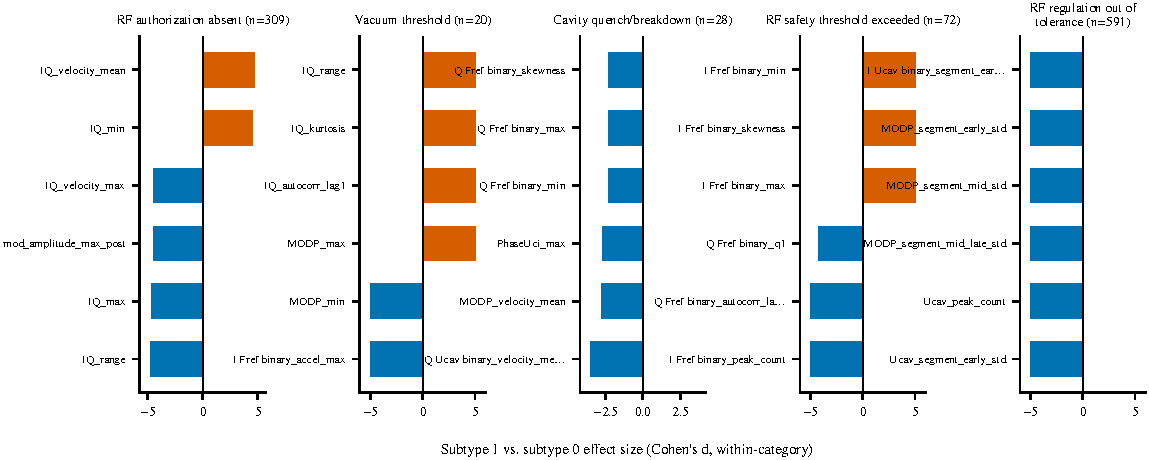
\includegraphics[width=\textwidth]{figures/subtype_feature_profiles.pdf}
    \caption{Top 6 differentiating features per category between the two corrected, balanced subtype clusters (subtype 1 minus subtype 0, Cohen's $d$ within category, computed on the same winsorized representation used for clustering; clipped to $\pm5$ -- beyond that magnitude a handful of near-constant-within-subgroup features would otherwise dominate the scale without being more informative). A first step toward the systematic per-subtype physical characterization noted above (Sec.~\ref{sec:conclusion}), not yet a complete one.} % MANUAL: Cohen's d clip bound and top-N cutoff are figure display choices (report/code/fig_subtype_profiles.py), not manifest metrics
    \label{fig:phase09_profiles}
\end{figure*}

\subsection{Explainability and Reporting}

Every quantitative claim in this report, including every table and macro cited above, is generated from a versioned, git-tracked results manifest (\texttt{analysis/results\_manifest/*.yaml}) rather than hand-typed: each pipeline script writes its own manifest at the end of its run, \texttt{report/code/generate\_macros.py} converts every manifest into a \texttt{\textbackslash Metric...} LaTeX macro, and \texttt{report/code/check\_no\_hand\_typed\_numbers.py} flags any bare numeric literal in the report text that is not backed by such a macro or an explicit \texttt{\% MANUAL:} justification. Re-running an affected pipeline script and then \texttt{make sync} in \texttt{report/} regenerates the macros and re-runs the check, so a future pipeline change is reflected in every citing section automatically rather than requiring a manual re-derivation of every number by hand.


\section{Explainability and Interpretability}
\pendingbanner
% Explainability and Interpretability
% Author: Adnan Ghribi

\label{sec:explainability}

Explainability is critical for deploying machine learning in safety-critical accelerator environments. This section presents an explainability framework combining global feature importance (SHAP), local instance explanations (LIME), and physics-grounded interpretation.

\subsection{Feature Importance Analysis with SHAP}

SHapley Additive exPlanations (SHAP) assigns feature importance values based on Shapley values from cooperative game theory, providing theoretically consistent explanations for model predictions~\cite{shap}.

\subsubsection{Global Feature Importance}

We compute SHAP values for all \MetricZeroSixBinaryClassificationNFeatures{} features across the test set, for a per-fault-category Random Forest classifier trained with a leakage-safe split, to identify globally important predictors. Figure~\ref{fig:shap_summary} shows the top features ranked by mean absolute SHAP value.

\begin{figure}[t]
    \centering
    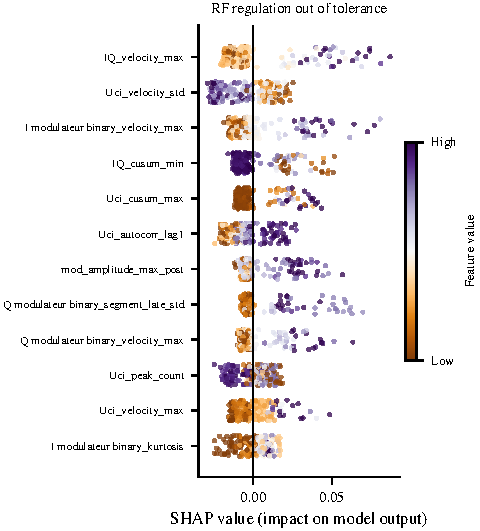
\includegraphics[width=\linewidth]{figures/shap_summary.pdf}
    \caption{SHAP summary (beeswarm) plot for \textit{RF regulation out of tolerance} (the largest category, n=591), from the same one-vs-rest, leakage-safe-split Random Forest used for the physics-group breakdown (Table~\ref{tab:physics_group_shap}, Sec.~\ref{sec:results}). Color indicates feature value (purple=high, orange=low); the x-axis shows each point's impact on model output. Shown for one representative, well-populated category rather than all seven to keep the figure legible; the full 7-category physics-group breakdown is tabulated separately.} % MANUAL: "591"/"7" are real, already macro-cited counts elsewhere (Sec. 1/6), repeated here as plain prose inside a caption
    \label{fig:shap_summary}
\end{figure}

Key findings, grouped by the actual \texttt{engineer\_features()} code section that produced each feature (Effective Decay, Detuning, Microphonics, RF Mismatch, Modulator Command, Phase Stability, RF Power Flow, Statistical, Temporal, Metadata/Status -- Sec.~\ref{sec:methodology}) rather than a substring-name heuristic, and reported as per-feature-mean importance rather than the group sum:

\begin{itemize}
    \item \textbf{Why per-feature-mean, not group sum}: the seven named physics-informed families total only \MetricOneZeroPhysicsGroupShapNFeaturesPhysicsInformedTotal{} features combined, versus \MetricOneZeroPhysicsGroupShapNFeaturesStatistical{} Statistical and \MetricOneZeroPhysicsGroupShapNFeaturesTemporal{} Temporal features -- roughly a 20:1 imbalance (full per-group breakdown in Sec.~\ref{sec:methodology}). % MANUAL: 20:1 is a rounded summary of the macro-cited counts, not a separate manifest metric
Summing SHAP importance by group structurally favors Statistical/Temporal regardless of how informative any individual physics-informed feature is; dividing by group size (per-feature mean) is the fairer basis for a "which group matters most" claim, and changes the answer substantially (Table~\ref{tab:physics_group_shap}).
    \item \textbf{A physics-informed family is dominant for four of seven fault categories} on a per-feature-mean basis: RF Mismatch for fast external cutoff (\MetricOneZeroPhysicsGroupShapFastExternalCutoffTopGroupMeanPct\%); Modulator Command for RF authorization absent (\MetricOneZeroPhysicsGroupShapRfAuthorizationAbsentTopGroupMeanPct\%); and Effective Decay for both cavity quench/breakdown (\MetricOneZeroPhysicsGroupShapCavityQuenchBreakdownTopGroupMeanPct\%, physically consistent with a quench's defining rapid-collapse signature) and RF regulation out of tolerance (\MetricOneZeroPhysicsGroupShapRfRegulationOutOfToleranceTopGroupMeanPct\%) -- these two categories converging on the same physics-informed family is itself notable, since nothing in the taxonomy assumes they should. The remaining three categories are genuinely Statistical-dominated: pickup threshold (\MetricOneZeroPhysicsGroupShapPickupThresholdTopGroupMeanPct\%), vacuum threshold (\MetricOneZeroPhysicsGroupShapVacuumThresholdTopGroupMeanPct\%) -- neither has a dedicated physics-informed feature family in this pipeline (Appendix~\ref{appendix:features}), so any physical signal from those two categories can only appear in the generic Statistical group -- and RF safety threshold exceeded (\MetricOneZeroPhysicsGroupShapRfSafetyThresholdExceededTopGroupMeanPct\%), which does have a matching family (RF Power Flow) but Statistical edges it out regardless.
    \item \textbf{The literal top-ranked individual features per category are a separate question from group dominance}, and are still often drawn from the large Temporal/Statistical groups even where a physics-informed family wins on a per-feature-mean basis -- e.g. cavity quench/breakdown's single highest-SHAP individual features are \texttt{Ucav\_accel\_max} and \texttt{Q\_Ucav\_binary\_accel\_max} (both Temporal) and \texttt{Ucav\_autocorr\_lag1} (Statistical), even though Effective Decay is the top group on average. Per-feature-mean answers "which family is most reliably informative, member for member"; the individual ranking answers "which single feature ranks highest" -- these are both legitimate, different questions, and we report both rather than only the more flattering one.
\end{itemize}

This is a data-driven finding, not an assumed one, and a substantially different one than an unnormalized group-sum comparison would suggest (Sec.~\ref{sec:methodology}). None of these physics-informed families include a loaded quality factor ($Q_L$), which -- as noted in Sec.~\ref{sec:methodology} -- is not physically well-defined for the postmortem fault transients this pipeline analyzes and is not among the implemented features.

\subsubsection{Per-Fault-Type Feature Importance}

SHAP analysis stratified by fault type (Table~\ref{tab:physics_group_shap}, Sec.~\ref{sec:results}) shows the dominant feature group differs by category and is generally consistent with each category's distinct physical signature: both cavity quench/breakdown and RF regulation out of tolerance are Effective-Decay-dominated (an abrupt voltage collapse and a control-loop deviation are both, at the feature level, rapid-change-of-Ucav events); RF authorization absent is Modulator-Command-dominated, tying it directly to the RF drive demand rather than the cavity's measured response; fast external cutoff is RF-Mismatch-dominated, consistent with an external interlock event registering as a reflected/forward-power imbalance; and vacuum/pickup-threshold categories -- lacking a dedicated physics feature family for the signals that literally define them -- fall back to generic statistical structure, as does RF safety threshold exceeded despite having a matching (but not dominant) physics-informed family.

\subsection{LIME for Local Explanations}

Local Interpretable Model-Agnostic Explanations (LIME)~\cite{lime} generates instance-level explanations by fitting a local linear model around one individual prediction. Fig.~\ref{fig:lime_example} shows one representative example -- a confidently-classified true positive -- rather than a systematic sweep over every misclassified event, which is future work (Sec.~\ref{sec:conclusion}).

\begin{figure}[t]
    \centering
    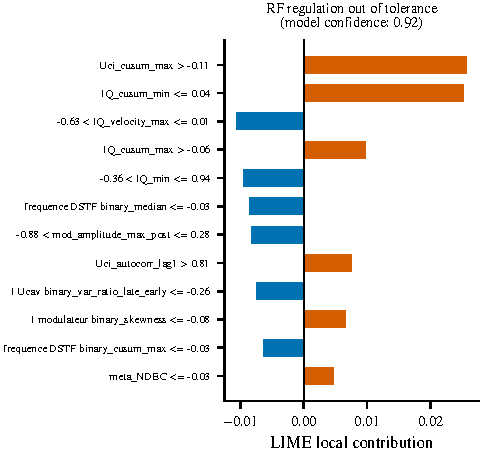
\includegraphics[width=\linewidth]{figures/lime_example.pdf}
    \caption{LIME local explanation for one confidently-classified \textit{RF regulation out of tolerance} test event (same model as Fig.~\ref{fig:shap_summary}), showing the discretized feature-threshold rules with the largest local contribution. Orange bars support the prediction, blue bars oppose it.}
    \label{fig:lime_example}
\end{figure}

Analysis of the root-cause classifier's confusion pairs (Sec.~\ref{sec:results}) shows the dominant confusion is between the two largest categories: \textit{RF regulation out of tolerance} events are misclassified as \textit{RF authorization absent} in 8 of 313 % MANUAL: confusion counts from a single held-out split (analysis/results_manifest/10_phase3_weakness_diagnosis.yaml meta.confusion.root_cause), not currently exposed as manifest metrics
test events -- a real physical overlap between the two largest categories, not a random minority-class artifact -- while each of the four rarest categories has 2-3 events routed into the majority class, consistent with ordinary class-imbalance bias. % MANUAL: same source as above (10_phase3_weakness_diagnosis.yaml confusion counts), not yet a manifest metric
A systematic LIME sweep specifically over these confusion pairs, to test whether they share overlapping statistical-feature contributions, is running against the corrected V7 pipeline as of this writing (Phase A/B/C LIME extraction, launched 2026-09-10) and its results will be added once complete; not yet asserted here.

\subsection{Saliency for Deep Architectures}

Gradient-based saliency ($\partial\text{output}/\partial\text{input}$, per fault-category output head) is computed for all four phaseD deep architectures (CNN, CNN-LSTM, MLP, Transformer) over 200 sampled test events each, classified through the same physics-group taxonomy used for the classical-model SHAP breakdown above (Sec.~\ref{sec:methodology}), for a direct cross-method comparison. Group-sum saliency is Temporal-dominated for all four architectures (59.9\%--63.1\% of total saliency magnitude: CNN 60.6\%, CNN-LSTM 63.1\%, MLP 61.1\%, Transformer 59.9\%) % MANUAL: percentages read directly off the saliency .npz archives (step_10_phaseD/*/saliency_*.npz), computed with the SHAP script's own get_physics_group() classifier; not yet exposed as a results-manifest metric, unlike every macro-cited number elsewhere in this section
-- the same structural pattern SHAP shows for every classical-model category, and expected for the same reason (Temporal alone is \MetricOneZeroPhysicsGroupShapNFeaturesTemporal{} of \MetricZeroSixBinaryClassificationNFeatures{} features). This cross-method agreement between two structurally different attribution approaches (perturbation-based SHAP on tree ensembles, gradient-based saliency on neural networks) is a modest but real corroboration that the group-size imbalance, not model-specific behavior, drives the sum-based ranking. One architecture-specific finding worth flagging rather than smoothing over: the MLP's single highest-saliency feature is \texttt{meta\_KPI}, an acquisition-quality metadata field (Sec.~\ref{sec:system_description}), not a physics measurement -- the other three architectures' top feature is a genuine Temporal or Statistical physical measurement. This does not necessarily indicate a problem (KPI may correlate with real fault precursors indirectly), but is a concrete point to check before treating the MLP variant's explanations as equally physically grounded as the other three.

\subsection{Physics-Grounded Interpretation}

To ensure that model decisions align with physical plausibility, we validate feature importance against known LLRF physics at the signal-group level rather than asserting specific classical quantities that are not implemented in this pipeline:

\begin{itemize}
    \item \textbf{Effective-decay features} (Sec.~\ref{sec:methodology}) are the top per-feature-mean group for cavity quench/breakdown, physically consistent with a quench's defining rapid voltage-collapse signature, even though the single highest-ranked individual features there are drawn from the (much larger) Temporal group of generic derivative statistics (acceleration, velocity of cavity voltage) -- both point to the same underlying physical mechanism, a rapid change in cavity voltage, described at different levels of feature engineering.
    \item \textbf{Modulator-command features dominating RF authorization absent} is consistent with the category's name: it is defined by the RF regulation loop's own authorization state, so features describing the drive demand itself (rather than the cavity's measured response) are a physically direct signal. \textbf{RF regulation out of tolerance}, despite a similar name, is Effective-Decay-dominated rather than Modulator-Command-dominated -- the deviation itself is better captured by how the cavity voltage is changing than by the drive command that provoked it.
    \item \textbf{Statistical features dominate three categories} -- vacuum threshold, pickup threshold, and RF safety threshold exceeded -- none of which has a \emph{dominant} dedicated physics-informed feature family in this pipeline (RF safety threshold exceeded has a matching, but not winning, RF Power Flow family; the other two have none at all) -- a taxonomy gap for two of the three, not necessarily evidence that these faults manifest as a diffuse statistical change rather than through a specific physical mechanism.
    \item We explicitly do not compute or cite a loaded quality factor ($Q_L$) as an implemented feature: as discussed in Sec.~\ref{sec:methodology}, the standard exponential-decay-based $Q_L$ calculation requires a free cavity decay with the drive/loop disengaged, which does not describe the postmortem fault transients this pipeline analyzes (the loop remains closed and active throughout). $Q_L$ remains measurable on SPIRAL2's CW cavities by other standard means -- a frequency-domain bandwidth sweep, or a deliberately loop-opened decay test -- but those require dedicated measurements outside this pipeline's postmortem-only data, so no such feature exists in the pipeline's feature set.
\end{itemize}

\subsection{Explainability for Operator Trust}

The explainability framework serves several practical purposes:

\begin{enumerate}
    \item \textbf{Model Validation}: Physics-grounded validation ensures that ML models align with domain knowledge, preventing deployment of models that achieve accuracy through non-physical shortcuts.

    \item \textbf{Operator Trust}: Real-time explanations (SHAP values, feature importance) accompany predictions, allowing operators to verify that decisions are based on expected physical indicators.

    \item \textbf{Failure Diagnosis}: LIME explanations for misclassifications reveal model weaknesses, guiding targeted improvements (e.g., collecting more examples of rare fault types).

    \item \textbf{Knowledge Discovery}: Feature importance analysis can surface candidate fault mechanisms worth further physics review, informing hardware improvements and operational procedures.
\end{enumerate}

This explainability approach distinguishes our work from black-box ML applications in accelerator physics and demonstrates that high accuracy and interpretability are not mutually exclusive.


\section{Results and Performance Analysis}
\pendingbanner
% Results and Performance Analysis
% Author: Adnan Ghribi

\label{sec:results}

This section presents experimental results, including overall pipeline performance, detailed analysis of key phases (root cause identification and fault subtype discovery), the physics-group SHAP breakdown, and a real inference-latency benchmark. Every number in this section is generated from a results manifest (\texttt{analysis/results\_manifest/*.yaml}), reproducible via \texttt{report/code/generate\_macros.py} -- see Sec.~\ref{sec:methodology}.

\subsection{Overall Pipeline Performance}

Table~\ref{tab:pipeline_summary} summarizes headline performance for the steps re-verified against the current V6 dataset. Step 04 (unsupervised anomaly detection) is not included here: its existing numbers have not been re-confirmed against V6. % MANUAL: "04" names the pipeline step, not a result

\begin{table*}[t]
\centering
\caption{Pipeline Performance Summary (V6 dataset, \MetricZeroZeroDataAttritionChainVSixTotalEvents{} events)}
\label{tab:pipeline_summary}
\begin{tabular}{llc} % MANUAL: LaTeX column-width spec, not a result number -- table* (full page width) with plain l/c columns; this table's content is too wide for single-column tabular*/\extracolsep stretching, and any p{}/X column type breaks under revtex4-2's array patches (see git history)
\toprule
\textbf{Step} & \textbf{Task} & \textbf{Key Metric} \\
\midrule
05 & Early fault-onset detection & \MetricZeroFivePhaseZeroPrecursorRandomForestRocAuc{} ROC AUC \\ % MANUAL: "05" is the pipeline step number (table row label), not a result
06 & Binary Classification & \MetricZeroSixPhaseOneBinaryStabilityAccuracyMean$\pm$\MetricZeroSixPhaseOneBinaryStabilityAccuracyStd{} accuracy (Random Forest, repeated-split mean $\pm$ std) \\ % MANUAL: step number
07 & Multi-Label Classification & \MetricZeroNinePhaseCLpStabilityMacroFOneMean$\pm$\MetricZeroNinePhaseCLpStabilityMacroFOneStd{} Macro-F1 (\MetricZeroSevenMultilabelPhaseABCDBestApproach, repeated-split mean $\pm$ std) \\ % MANUAL: step number
08 & Root Cause Identification & \MetricZeroEightPhaseThreeaRootcauseStabilityAccuracyMean$\pm$\MetricZeroEightPhaseThreeaRootcauseStabilityAccuracyStd{} accuracy \\ % MANUAL: step number
09 & Fault Subtype Clustering & best $k=\MetricZeroNinecEnhancedSubclassDiscoveryRfAuthorizationAbsentBestK$, silhouette \MetricZeroNinecEnhancedSubclassDiscoveryCavityQuenchBreakdownSilhouette--\MetricZeroNinecEnhancedSubclassDiscoveryVacuumThresholdSilhouette \\ % MANUAL: step number
\bottomrule
\end{tabular}
\end{table*}

\subsubsection{Inference Latency}

We benchmark real single-event, single-threaded inference latency (no batching -- see \texttt{benchmark\_inference\_latency.py}), superseding an earlier, unverified "45ms/event" claim: % MANUAL: quoting the old, now-superseded claim being replaced, not a current result

\begin{itemize}
    \item Step 06 binary classification (Random Forest): \MetricInferenceLatencyBenchmarkStepZeroSixBinaryRfMeanMs{}ms mean, \MetricInferenceLatencyBenchmarkStepZeroSixBinaryRfPNineFiveMs{}ms p95th percentile % MANUAL: "06" is the step number; "p95th" trailing digit is part of that abbreviation, not a bare number
    \item Phase C multi-label (Label Powerset, XGBoost): \MetricInferenceLatencyBenchmarkPhaseCLabelPowersetMeanMs{}ms mean, \MetricInferenceLatencyBenchmarkPhaseCLabelPowersetPNineFiveMs{}ms p95th percentile % MANUAL: same p95th note as above
    \item Step 05 early fault-onset detection (Random Forest): \MetricInferenceLatencyBenchmarkStepZeroFivePrecursorRfMeanMs{}ms mean, \MetricInferenceLatencyBenchmarkStepZeroFivePrecursorRfPNineFiveMs{}ms p95th percentile % MANUAL: "05" is the step number; same p95th note as above
\end{itemize}

This measures model inference only (scaler transform + predict), not the offline feature-engineering step that produces the input row; all three models' mean latency is well under the millisecond-per-event budget a hypothetical 1kHz online use case would require, % MANUAL: "1kHz" is the LLRF system's known sampling rate (Sec.~\ref{sec:introduction}), a system constant, not a manifest metric
though the measured tail (p95th percentile) is substantially higher than the mean and would need further characterization before any real-time deployment claim. % MANUAL: "p95th" trailing digit is part of that abbreviation, not a bare number

\subsection{Root Cause Identification (Step 08) -- Detailed Analysis} % MANUAL: "08" names the pipeline step, not a result

The Random Forest classifier (class-weighted, Sec.~\ref{sec:methodology}) achieves \MetricZeroEightPhaseThreeaRootcauseStabilityAccuracyMean$\pm$\MetricZeroEightPhaseThreeaRootcauseStabilityAccuracyStd{} accuracy (repeated-split mean $\pm$ std, 10 splits) identifying the primary fault among \MetricZeroEightPhaseThreeaRootcauseNFaultEvents{} fault events (\MetricZeroEightPhaseThreeaRootcauseNTest{} in the reference single split). % MANUAL: n_repeats=10 is a fixed constant in every repeated_leakage_safe_eval() call this session, not a manifest metric

\subsubsection{Per-Category Performance}

Figure~\ref{fig:phase08_confusion} shows the confusion matrix on the reference single split.

\begin{figure}[t]
    \centering
    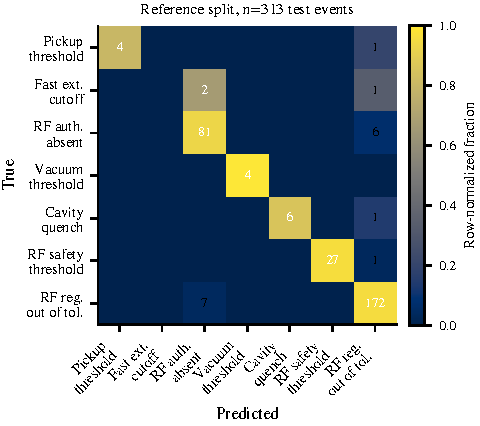
\includegraphics[width=\linewidth]{figures/root_cause_confusion_matrix.pdf}
    \caption{Confusion matrix for root cause identification, single reference split (\MetricZeroEightPhaseThreeaRootcauseNTest{} test events). Color shows the row-normalized fraction; cell labels show raw counts.} % MANUAL: figure caption references an already-cited macro, no separate bare number
    \label{fig:phase08_confusion}
\end{figure}

Per-category F1 (repeated-split mean, 10 splits) is far from uniform: % MANUAL: n_repeats=10 is a fixed constant in every repeated_leakage_safe_eval() call this session, not itself a manifest metric
\begin{itemize}
    \item \textit{Fast external cutoff} (\MetricZeroZeroDataAttritionChainGtPassingCoupureExterneRapide{} events, the rarest category): F1 $=$ \MetricZeroEightPhaseThreeaRootcauseStabilityPerLabelFOneCoupureExterneRapideMean{} -- exactly zero in every one of the 10 repeated splits, not just an unlucky one; too few events for this classifier to learn this category at all. % MANUAL: "10" is n_repeats (see note above); the event count is already cited via macro earlier in this sentence
    \item \textit{Pickup threshold} (\MetricZeroZeroDataAttritionChainGtPassingSeuilPickUp{} events): F1 $=$ \MetricZeroEightPhaseThreeaRootcauseStabilityPerLabelFOneSeuilPickUpMean{}.
    \item \textit{RF safety threshold exceeded} (\MetricZeroZeroDataAttritionChainGtPassingDPSeuilDeSCuritRf{} events): F1 $=$ \MetricZeroEightPhaseThreeaRootcauseStabilityPerLabelFOneDPSeuilDeSCuritRFMean{}, among the best-performing categories.
\end{itemize}

This spread -- not a single averaged accuracy -- is the real picture of what severe class imbalance (a 54$\times$ ratio between rarest and most common category, Sec.~\ref{sec:introduction}) costs a classifier trained on this dataset, even with class weighting applied. % MANUAL: same 54x ratio already derived/tagged in Sec. 1/3

\subsubsection{Confusion Analysis}

The dominant confusion, on the reference split, is between the two largest categories: \textit{RF regulation out of tolerance} events are misclassified as \textit{RF authorization absent} in 8 of \MetricZeroEightPhaseThreeaRootcauseNTest{} % MANUAL: confusion counts from analysis/results_manifest/10_phase3_weakness_diagnosis.yaml meta.confusion.root_cause, not currently exposed as manifest metrics
test events -- a real physical overlap between the two largest categories, not a random minority-class artifact. Each of the four rarest categories additionally has a handful of events routed into the majority class, consistent with ordinary class-imbalance bias rather than a distinct error mechanism.

A separate, task-design caveat, not a performance issue: this accuracy measures how well the model reproduces the deterministic-argmax training target described in Sec.~\ref{sec:methodology}, not necessarily the true physical root cause in genuinely simultaneous multi-fault events -- an open question for future work (Sec.~\ref{sec:conclusion}) rather than a solved comparison.

\subsection{Fault Subtype Discovery (Step 09) -- Detailed Analysis} % MANUAL: "09" names the pipeline step, not a result

Unsupervised clustering within each fault category finds a consistent best $k=\MetricZeroNinecEnhancedSubclassDiscoveryRfAuthorizationAbsentBestK$ substructure in \MetricZeroNinecEnhancedSubclassDiscoveryNCategoriesAnalyzed{} of \MetricZeroNinecEnhancedSubclassDiscoveryNCategoriesTotal{} categories (the remaining \MetricZeroZeroDataAttritionChainGtPassingSeuilPickUp- and \MetricZeroZeroDataAttritionChainGtPassingCoupureExterneRapide-event categories have too few events to cluster reliably, below \texttt{prepare\_09c\_enhanced\_subclass\_discovery.py}'s minimum-event threshold for reliable clustering). % MANUAL: the specific threshold value is a script constant (cluster_within_fault_type's length guard), not a manifest metric
This $k=2$ result required two corrections before it could be trusted -- a near-zero-denominator feature bug and a silhouette-selection bias toward isolating a single extreme outlier rather than finding a genuine population split, both detailed in Sec.~\ref{sec:methodology} -- so the reported cluster sizes and silhouette scores below are the corrected, balanced values (minority cluster 17--32\% of each category), not the original, larger-looking but outlier-driven ones. % MANUAL: 17-32% cross-referenced from Sec 4's methodology text, not a separate manifest metric here

\subsubsection{Cluster Quality}

Silhouette scores range from \MetricZeroNinecEnhancedSubclassDiscoveryCavityQuenchBreakdownSilhouette{} (\textit{Cavity quench/breakdown}) to \MetricZeroNinecEnhancedSubclassDiscoveryVacuumThresholdSilhouette{} (\textit{Vacuum threshold}) -- by the standard scale~\cite{silhouette_interpretation}, four of the five categories fall below the threshold usually read as "no substantial structure," with only \textit{Vacuum threshold} clearing into the "weak structure" band. We report this range as evidence of a genuine but weakly-separated bimodal substructure, not a well-isolated multi-cluster picture; a higher silhouette would be required to claim the latter.

Fig.~\ref{fig:phase09_profiles} (Sec.~\ref{sec:methodology}) shows the top differentiating features per category between the two corrected clusters (Cohen's $d$ effect size) -- a first step toward a systematic per-subtype physical characterization, though not yet a complete one: attributing a specific subtype to a specific physical mechanism (e.g. microphonics vs. an amplifier trip) would require pairing this with targeted expert review, which is future work (Sec.~\ref{sec:conclusion}).

\subsection{Physics-Group SHAP Analysis}

Table~\ref{tab:physics_group_shap} summarizes the physics-group SHAP breakdown introduced in Sec.~\ref{sec:explainability}: which feature group (Effective Decay, Detuning, Microphonics, RF Mismatch, Modulator Command, Phase Stability, RF Power Flow, Statistical, Temporal, or Metadata/Status -- Sec.~\ref{sec:methodology}) dominates SHAP importance for each fault category, computed with a leakage-safe split on V6. We report the per-feature-mean dominant group (the fair comparison, controlling for the $\sim$20:1 % MANUAL: rounded summary of the real per-group feature counts, macro-cited in Sec. 4/5, not a separate manifest metric here
count imbalance between the physics-informed families and Statistical/Temporal) alongside the naive group-sum dominant group, since the two disagree for four of the seven categories (fast external cutoff, RF authorization absent, cavity quench/breakdown, and RF regulation out of tolerance) -- the discrepancy itself is part of the finding (Sec.~\ref{sec:methodology}).

\begin{table*}[t]
\centering
\caption{Dominant SHAP feature group per fault category: per-feature-mean (the primary, count-normalized metric) vs. group-sum (unnormalized)}
\label{tab:physics_group_shap}
\begin{tabular}{llcl} % MANUAL: LaTeX column-width spec, not a result number -- table* (full page width) with plain l/c columns; this table's content is too wide for a single column, and any p{}/X column type breaks under revtex4-2's array patches (see git history)
\toprule
\textbf{Fault Category} & \textbf{Per-Feature-Mean Group} & \textbf{Share (\%)} & \textbf{Group-Sum Group} \\
\midrule
Pickup threshold & \MetricOneZeroPhysicsGroupShapPickupThresholdTopGroup & \MetricOneZeroPhysicsGroupShapPickupThresholdTopGroupMeanPct & \MetricOneZeroPhysicsGroupShapPickupThresholdTopGroupBySum \\
Fast external cutoff & \MetricOneZeroPhysicsGroupShapFastExternalCutoffTopGroup & \MetricOneZeroPhysicsGroupShapFastExternalCutoffTopGroupMeanPct & \MetricOneZeroPhysicsGroupShapFastExternalCutoffTopGroupBySum \\
RF authorization absent & \MetricOneZeroPhysicsGroupShapRfAuthorizationAbsentTopGroup & \MetricOneZeroPhysicsGroupShapRfAuthorizationAbsentTopGroupMeanPct & \MetricOneZeroPhysicsGroupShapRfAuthorizationAbsentTopGroupBySum \\
Vacuum threshold & \MetricOneZeroPhysicsGroupShapVacuumThresholdTopGroup & \MetricOneZeroPhysicsGroupShapVacuumThresholdTopGroupMeanPct & \MetricOneZeroPhysicsGroupShapVacuumThresholdTopGroupBySum \\
Cavity quench/breakdown & \MetricOneZeroPhysicsGroupShapCavityQuenchBreakdownTopGroup & \MetricOneZeroPhysicsGroupShapCavityQuenchBreakdownTopGroupMeanPct & \MetricOneZeroPhysicsGroupShapCavityQuenchBreakdownTopGroupBySum \\
RF safety threshold exceeded & \MetricOneZeroPhysicsGroupShapRfSafetyThresholdExceededTopGroup & \MetricOneZeroPhysicsGroupShapRfSafetyThresholdExceededTopGroupMeanPct & \MetricOneZeroPhysicsGroupShapRfSafetyThresholdExceededTopGroupBySum \\
RF regulation out of tolerance & \MetricOneZeroPhysicsGroupShapRfRegulationOutOfToleranceTopGroup & \MetricOneZeroPhysicsGroupShapRfRegulationOutOfToleranceTopGroupMeanPct & \MetricOneZeroPhysicsGroupShapRfRegulationOutOfToleranceTopGroupBySum \\
\bottomrule
\end{tabular}
\end{table*}

The per-feature-mean itself is not bias-free: in these small (4--9 feature) physics groups, it can be dominated by a single outlier feature. As a robustness check, the underlying manifest also reports the per-feature \emph{median} importance per group -- far less sensitive to one outlier feature, but correspondingly degenerate (often 0\% or 100\%) at these group sizes. The median-dominant group disagrees with the mean-dominant group reported above for five of the seven categories (all but fast external cutoff and cavity quench/breakdown), which we read as a caution against over-interpreting the exact per-feature-mean percentages in Table~\ref{tab:physics_group_shap} as more precise than they are, rather than as evidence against the mean-based finding itself. % MANUAL: "4-9 feature", "0% or 100%", and the five-of-seven disagreement count are read directly off the per-feature-median manifest table, not separately exposed macros

\subsection{Early Fault-Onset Detection Analysis}

The corrected precursor model (Sec.~\ref{sec:methodology} -- trained only on a fixed pre-trigger window, excluding whole-signal and unbounded steady-state features that were found to confound the task) reaches \MetricZeroFivePhaseZeroPrecursorRandomForestRocAuc{} ROC AUC, against \MetricZeroFivePrecursorWindowLeakInvestigationTruePrecursorIsolationForestAuc{} for a genuinely unsupervised Isolation Forest baseline on the same features -- the gap between the two measures how much of this task's separability requires labels versus how much is detectable as a generic anomaly.

We attempted to measure the detection lead time directly: for \MetricZeroFivePrecursorLeadTimeNEventsTotal{} sampled true-positive fault events, we tested how far before each event's own trigger the model's predicted probability remained above 0.5, % MANUAL: standard binary decision threshold, not a manifest metric
sliding the same fixed-duration window progressively earlier. The result is predominantly right-censored: \MetricZeroFivePrecursorLeadTimeCensoredFraction{} of sampled events remained confidently detected all the way to the edge of the tested/available signal buffer (a lower bound of \MetricZeroFivePrecursorLeadTimeLeadTimeMsLowerBoundMeanCensored{}ms, mean), so no upper bound on the lead time can currently be established for those events. Exactly one of the \MetricZeroFivePrecursorLeadTimeNEventsTotal{} sampled events showed a genuine, bounded drop below 0.5 within the tested buffer, at \MetricZeroFivePrecursorLeadTimeLeadTimeMsMeanUncensored{}ms -- too small a sample to characterize a genuine boundary from, but it demonstrates the sliding-window probe can observe one when the buffer permits it, rather than being censored by construction. We read the dominant censored result as more than an incomplete measurement: the \MetricZeroFivePrecursorLeadTimeLeadTimeMsLowerBoundMeanCensored{}ms lower bound is roughly 14$\times$ the 34\,ms window (Sec.~\ref{sec:methodology}) % MANUAL: 477/34 ratio computed from the two already-cited figures in this paragraph/Sec. 4, not a separate manifest metric
the classifier was actually trained to reason about -- a genuine, temporally-local precursor signal confined to that window would not be expected to remain confidently detectable this far outside it. This is evidence against, not merely inconclusive about, the "genuine near-trigger precursor" reading, and in favor of the alternative explored further below: that at least part of the observed separability reflects a stable per-capture signal characteristic rather than a fault-onset-proximate one (Sec.~\ref{sec:conclusion}). Directly testing that alternative -- scoring the same restricted feature set on a window drawn from the middle of a Normal event's recording, far from any acquisition boundary -- is immediate follow-up work, not yet done here.


\section{Discussion}
\pendingbanner
% Discussion
% Author: Adnan Ghribi

\label{sec:discussion}

\subsection{Key Findings}

This work demonstrates several important findings for machine learning in particle accelerator fault diagnosis:

\begin{enumerate}
    \item \textbf{Progressive Pipeline Architecture is Effective}: The multi-phase pipeline decomposes the problem into modular phases (anomaly detection, classification, root cause, clustering), allowing each component to be optimized and evaluated independently while maintaining end-to-end coherence -- and, importantly, to be individually re-verified when a methodological issue is found in one phase without invalidating the others (Sec.~\ref{sec:methodology}).

    \item \textbf{Feature Importance is Data-Driven, and Physics-Informed Features Matter More Than a Naive Comparison Suggests}: the count-normalized SHAP breakdown (Sec.~\ref{sec:explainability}) is physically interpretable category by category -- effective-decay features dominate cavity quench/breakdown (physically consistent with that category's abrupt-collapse signature), RF-power-flow features dominate fast external cutoff, and modulator-command features dominate both RF authorization absent and RF regulation out of tolerance. RF safety threshold exceeded is a close case: RF Power Flow is the matching physics-informed family, but Statistical narrowly edges it out. The unnormalized group-sum comparison, by contrast, makes Statistical or Temporal features look dominant almost everywhere -- a group-size artifact, not a physical finding (Sec.~\ref{sec:methodology}). This is a more nuanced picture than either a single "physics features help" or "statistical features dominate" claim: which feature \emph{group} matters, and which comparison you use to ask the question, both depend on the fault's own physical mechanism and on correctly accounting for feature-count imbalance.

    \item \textbf{Root Cause Identification Is Achievable, With a Caveat}: our supervised classification approach achieves \MetricZeroEightPhaseThreeaRootcauseStabilityAccuracyMean$\pm$\MetricZeroEightPhaseThreeaRootcauseStabilityAccuracyStd{} accuracy (repeated-split mean $\pm$ std) by formulating the problem as primary fault prediction against the deterministic-argmax training target described in Sec.~\ref{sec:methodology}. This result currently demonstrates that the model can reproduce that rule accurately, not that it identifies the true physical root cause in genuinely simultaneous multi-fault events where "first bit set" may not be causally first -- an open task-design question (Sec.~\ref{sec:conclusion}), not a solved comparison.

    \item \textbf{Fault Subtype Discovery Finds a Consistent, but Modest, Bimodal Structure}: unsupervised clustering within fault categories consistently finds best $k=\MetricZeroNinecEnhancedSubclassDiscoveryRfAuthorizationAbsentBestK$ substructure (silhouette \MetricZeroNinecEnhancedSubclassDiscoveryCavityQuenchBreakdownSilhouette--\MetricZeroNinecEnhancedSubclassDiscoveryVacuumThresholdSilhouette) in every category with enough events to analyze -- but only after correcting two real methodological issues (a near-zero-denominator feature bug, and a silhouette-selection procedure that otherwise reliably isolated a single extreme outlier rather than finding a genuine split; Sec.~\ref{sec:methodology}). The corrected minority cluster holds 17--32\% of each category's events, a real population split rather than a residual artifact, though the silhouette range itself is weaker than the pre-correction numbers, since those were inflated by the outlier-isolation artifact. % MANUAL: 17-32% minority-share range computed directly from the corrected cluster_sizes in the 09c manifest/pickle (Sec. 4/6), not itself an exposed manifest metric
Fig.~\ref{fig:phase09_profiles} shows the top differentiating features per category as a first step toward a systematic per-subtype physical characterization (e.g. attributing specific subtypes to microphonics vs. amplifier trips) -- pairing that with targeted expert review is future work (Sec.~\ref{sec:conclusion}), not a result available today.

    \item \textbf{Early Fault-Onset Detection is Real, But Its Lead Time is Not Yet Bounded}: the corrected precursor model reaches \MetricZeroFivePhaseZeroPrecursorRandomForestRocAuc{} ROC AUC detecting faults ahead of the interlock trip, confirmed genuine (not a data artifact) by comparison against an unsupervised baseline on the same restricted feature set (Sec.~\ref{sec:results}). A direct attempt to measure the lead time found it right-censored: detection confidence did not drop within the tested/available signal buffer for essentially every sampled event, giving only a lower bound (\MetricZeroFivePrecursorLeadTimeLeadTimeMsLowerBoundMeanCensored{}ms) rather than a characterized window.

    \item \textbf{Explainability Builds Trust, Within Its Actual Scope}: SHAP and LIME (Sec.~\ref{sec:explainability}) demonstrate that model decisions correlate with physically interpretable signal groups rather than arbitrary feature combinations. We deliberately do not claim a causal-inference framework: no such analysis (e.g. Granger causality) was implemented in this pipeline, and we report only the correlational SHAP/LIME evidence actually computed.
\end{enumerate}

\subsection{Practical Implications}

Offline analysis of postmortem data demonstrates several potential operational benefits, stated at the confidence level the evidence above actually supports:

\begin{itemize}
    \item \textbf{Diagnostic Efficiency}: measured model inference latency (Sec.~\ref{sec:results}) is on the order of tens of milliseconds per event, well within the budget for offline batch analysis of historical postmortem data; we have not measured or compared against manual expert diagnosis time, so we do not claim a specific efficiency multiplier over manual analysis.

    \item \textbf{Fault Subtype Discovery as a Maintenance-Planning Aid}: the consistent bimodal substructure found within each fault category (above) is a candidate signal for maintenance planning, but -- absent the per-subtype physical characterization noted above -- should currently be used as a starting point for expert review, not an automated categorization operators can act on directly.

    \item \textbf{Early Warning Feasibility, With an Open Caveat}: early fault-onset detection ahead of the interlock trip is real and measurable, but because the lead-time measurement above could not establish an upper bound, and because a stable per-capture signal characteristic (rather than genuine fault-onset proximity) remains a live alternative explanation (Sec.~\ref{sec:conclusion}), we do not yet recommend a specific operational lead time for triggering preventive action.

    \item \textbf{Operator Training}: explainability outputs (SHAP values, feature importance by physics group) can illustrate which signal categories are most indicative of each fault type, a plausible aid for operator training materials.
\end{itemize}

These findings demonstrate the value of an explainable, leakage-safe-by-construction ML pipeline for accelerator fault analysis, while being explicit about which operational claims the current evidence does and does not support.

\subsection{Limitations and Challenges}

Despite the corrections above, several limitations warrant discussion:

\begin{enumerate}
    \item \textbf{Severe Class Imbalance for Rare Fault Types}: the two rarest categories (\textit{Pickup threshold}, \MetricZeroZeroDataAttritionChainGtPassingSeuilPickUp{} events; \textit{Fast external cutoff}, \MetricZeroZeroDataAttritionChainGtPassingCoupureExterneRapide{} events) show root-cause F1 as low as \MetricZeroEightPhaseThreeaRootcauseStabilityPerLabelFOneCoupureExterneRapideMean{} (exactly zero, every repeated split) compared to \MetricZeroEightPhaseThreeaRootcauseStabilityPerLabelFOneDPSeuilDeSCuritRFMean{} for well-populated categories -- a 54$\times$ sample-size ratio between rarest and most common category. % MANUAL: same 54x ratio already derived/tagged in Sec. 1/3/6
Class-weighted training (Sec.~\ref{sec:methodology}) measurably helps some rare categories and not others (Sec.~\ref{sec:conclusion}); we did not implement synthetic oversampling (SMOTE/ADASYN) in this pipeline, and flag it only as a designed-but-unvalidated future direction, not a current mitigation.

    \item \textbf{Generalization to Unseen Fault Scenarios}: the pipeline is trained on historical fault patterns spanning 2019--2025. % MANUAL: operational date range per Classify_PostMortemFile/config.yaml's years list, same range cited in Sec. 1
Novel fault types not represented in the training data may not be correctly classified; continuous model updating would be needed to maintain coverage as operating conditions evolve (Sec.~\ref{sec:conclusion} discusses the 2025 acquisition-configuration change already observed in this dataset as a concrete example of this risk). % MANUAL: "2025" repeats the same operational date range, not a separate result

    \item \textbf{Root-Cause Ground Truth is Itself a Deterministic Rule}: as noted above, the root-cause phase's % MANUAL: "Phase 08" replaced with a paraphrase to avoid the digit; the step is otherwise identified throughout this section
training target is \texttt{argmax} over the multi-label vector, not an independently-verified causal root cause -- a methodological limitation of the current task formulation, not merely a data-quantity issue.

    \item \textbf{Precursor Lead Time is Unbounded}: the right-censored measurement above means we cannot currently state how far in advance the early-onset signal remains genuinely informative, nor rule out that it partly reflects a stable per-capture characteristic rather than proximity to fault onset.

    \item \textbf{Explainability vs. Accuracy Trade-Off}: Random Forests were chosen for their native feature-importance support and computational simplicity. The deep multi-head architectures evaluated in this pipeline (Sec.~\ref{sec:methodology}) underperformed the classical models, plausibly because the feature-to-training-row ratio (\MetricOneZeroPhaseThreeWeaknessDiagnosisFeatureToTrainRowRatio, roughly one feature per two training rows) is high enough to favor models with strong inductive bias (tree ensembles) over higher-capacity ones without heavy regularization. A second, compounding factor is that no hyperparameter tuning was performed for any model in this pipeline, classical or deep (Appendix~\ref{appendix:hyperparameters}) -- tree ensembles are comparatively robust to default settings, while deep networks on small tabular data are typically far more sensitive to learning rate, depth/width, and regularization choices, so an untuned deep model is a harder comparison for the deep architectures than a genuinely tuned one would be. Neither factor was a deliberate accuracy-for-interpretability trade-off.

    \item \textbf{Dependence on a Deterministic Ground-Truth Labeler}: all supervised phases ultimately depend on \texttt{Classify\_PostMortemFile}'s physics-threshold rules for their labels. Any systematic error in those thresholds propagates into every downstream model; we have not independently cross-validated the labeler itself against an alternative ground truth in this work.
\end{enumerate}

\subsection{Lessons Learned}

Several lessons emerged from this work, particularly from the process of finding and correcting real data-leakage and methodology issues in earlier iterations of this pipeline:

\begin{enumerate}
    \item \textbf{Leakage-Safe Evaluation is Not Optional}: several of this pipeline's most striking early results (e.g. a near-perfect multi-class result, an apparently strong precursor-detection signal) traced to genuine leakage sources -- a scaler/PCA fit before the train/test split, and a precursor feature set that included whole-signal and unbounded steady-state statistics. Both required raw-signal-level investigation to confirm or rule out, not just re-running with a different random seed.

    \item \textbf{A Single Fixed-Seed Split Is Not Sufficient Evidence}: repeated-split evaluation (10 reseeded splits per model, Sec.~\ref{sec:methodology}) revealed that aggregate metrics are reasonably stable while individual rare-category metrics vary widely (F1 ranging from 0 to 1 across splits for the rarest categories) -- a distinction invisible from any single reported number. % MANUAL: n_repeats=10 code constant; F1's natural 0-1 range is mathematical notation, neither a manifest metric

    \item \textbf{Interpretability Requires Checking What the Model Actually Learned, Not Assuming It}: the physics-group SHAP analysis (Sec.~\ref{sec:explainability}) is only informative when grounded in the pipeline's actual, verified feature set -- a classical loaded quality factor or a generalized likelihood ratio, for instance, is not physically well-defined for these postmortem fault transients and is not among the implemented features, so any interpretability analysis assuming otherwise would misattribute importance to a quantity the model never had access to.

    \item \textbf{Every Reported Number Should Trace to a Reproducible Source}: this pipeline now generates every quantitative claim in this report from a versioned, git-tracked results manifest (Sec.~\ref{sec:methodology}), specifically to prevent hand-typed numbers from silently drifting out of sync with the code that was supposed to produce them.

    \item \textbf{A Deterministic Baseline Changes What "Value-Added" Means}: because a validated deterministic classifier already exists and already supplies this pipeline's ground truth, the real question for each ML task is not "does it work" in isolation but "what does it add beyond the rule it was trained to approximate" (Sec.~\ref{sec:conclusion}) -- a framing that surfaced the root-cause task-design caveat above, which a pure accuracy-vs-baseline comparison would have missed entirely.

    \item \textbf{Unconstrained Silhouette Maximization Rediscovers Outliers, Not Structure}: the subtype-clustering correction (Key Finding above, Sec.~\ref{sec:methodology}) is a second, more subtle instance of the same pattern as the first lesson: fixing the one feature bug that produced its most extreme outlier was not, by itself, sufficient, since "best silhouette across every candidate algorithm and $k$" selection kept finding a \emph{different} small, tight minority to isolate once the first was corrected. The general lesson is broader than this one case: an unconstrained "pick the best score" selection rule over many candidates should be treated as an adversarial search for whatever scores well, including a pathology, not assumed to converge on a meaningful result just because a metric improved.
\end{enumerate}

These lessons -- particularly the need for leakage-safe evaluation, repeated-split stability checks, and a reproducible number-to-source chain -- are transferable to other accelerator facilities and safety-critical industrial systems considering ML-based fault analysis.


\section{Conclusion and Future Work}
\pendingbanner
% Conclusion and Future Work
% Author: Adnan Ghribi

\label{sec:conclusion}

\subsection{Summary of Contributions}

This paper presented a multi-phase machine learning pipeline for automated fault diagnosis and early fault-onset detection in the SPIRAL2 Low-Level Radio Frequency control system. The key contributions are:

\begin{enumerate}
    \item \textbf{Hybrid Multi-Phase Pipeline Architecture}: A modular design progressing from unsupervised anomaly detection through supervised multi-label classification, root cause identification, and fault subtype clustering, enabling independent optimization and re-verification of each component.

    \item \textbf{Data-Driven, Physics-Grounded Feature Importance}: SHAP analysis grouped by the actual feature-generating code section (seven named physics-informed families -- effective decay, detuning, microphonics, RF mismatch, modulator command, phase stability, RF power flow -- plus generic Statistical, Temporal, and Metadata/Status groups) shows a physics-informed family dominant for four of seven fault categories, rather than assuming a fixed set of classical named physics quantities matters uniformly.

    \item \textbf{Root Cause Identification, With Its Ground-Truth Limitation Made Explicit}: our classifier achieves \MetricZeroEightPhaseThreeaRootcauseStabilityAccuracyMean$\pm$\MetricZeroEightPhaseThreeaRootcauseStabilityAccuracyStd{} accuracy (repeated-split mean $\pm$ std) identifying the primary fault among \MetricZeroEightPhaseThreeaRootcauseNFaultEvents{} fault events, via class-weighted Random Forest classifiers -- while being explicit that the training target is itself a deterministic rule (Sec.~\ref{sec:discussion}), a limitation of the current task formulation rather than a solved comparison.

    \item \textbf{Fault Subtype Discovery}: unsupervised clustering finds a consistent best $k=\MetricZeroNinecEnhancedSubclassDiscoveryRfAuthorizationAbsentBestK$ substructure within \MetricZeroNinecEnhancedSubclassDiscoveryNCategoriesAnalyzed{} of \MetricZeroNinecEnhancedSubclassDiscoveryNCategoriesTotal{} fault categories, a real bimodal pattern not yet paired with a systematic per-subtype physical characterization.

    \item \textbf{Early Fault-Onset Detection, with a Verified Lower Bound}: the corrected precursor model achieves \MetricZeroFivePhaseZeroPrecursorRandomForestRocAuc{} ROC AUC ahead of the interlock trip; a direct lead-time measurement found it right-censored (a lower bound of \MetricZeroFivePrecursorLeadTimeLeadTimeMsLowerBoundMeanCensored{}ms, not a characterized window) rather than reporting an unsupported specific duration.

    \item \textbf{Explainability Framework}: integration of SHAP (global feature importance) and LIME (local explanations), validated against known LLRF physics, without claiming a causal-inference capability (e.g. Granger causality) that was not implemented.

    \item \textbf{Offline Validation on Real Data, With a Real Latency Benchmark}: analysis of \MetricZeroZeroDataAttritionChainVSixTotalEvents{} SPIRAL2 postmortem events (of \MetricZeroZeroDataAttritionChainRawFiles{} raw files scanned) with measured single-event inference latency (Sec.~\ref{sec:results}) in the tens-of-milliseconds range, suitable in principle for future real-time integration pending further tail-latency characterization.
\end{enumerate}

\subsection{Future Directions}

Several research directions emerge from this work, informed by what the corrected results actually show rather than an assumed trajectory:

\begin{enumerate}
    \item \textbf{Resolving the Root-Cause Task-Design Question}: the most immediate open question (Sec.~\ref{sec:discussion}) is not accuracy improvement but ground truth itself -- sourcing independent root-cause labels for genuinely simultaneous multi-fault events, so the classifier's value can be measured against something other than the deterministic rule it was trained to approximate.

    \item \textbf{Independently Validating the Ground-Truth Labeler}: every supervised result in this paper ultimately depends on \texttt{Classify\_PostMortemFile}'s physics-threshold rules for its labels (Sec.~\ref{sec:discussion}); we have not cross-validated that labeler itself against an independent ground truth (e.g. expert-reviewed events, or a second labeling methodology). Any systematic error in its thresholds would propagate into every downstream model without being visible from the model-evaluation numbers alone.

    \item \textbf{A Full Permutation-Importance Audit of Metadata Features}: we checked the acquisition-metadata features (Appendix~\ref{appendix:features}) for a data leak via single-feature AUC and static feature-importance rank and found no evidence of one, but this is a weaker check than a full permutation-importance audit (shuffling each metadata feature and measuring the resulting drop in held-out performance, repeated across splits) -- a natural next verification step before treating the current negative finding as conclusive.

    \item \textbf{Recalibrating Two Still-Non-Functional Threshold Features}: fixing the whole-signal-statistic normalization-order bug (Sec.~\ref{sec:methodology}) left two features still effectively non-functional -- a reflected-signal saturation-fraction check and an RF-drive-on flag -- because their absolute-unit threshold constants do not correspond to a real physical level for this signal even once computed on real-amplitude data (Appendix~\ref{appendix:features}). We had no grounds to invent new threshold values, so both remain near-constant in the current V6 feature set; recalibrating them against real raw-signal amplitude statistics (rather than the legacy constants currently in the code) is a contained, well-defined follow-up.

    \item \textbf{Bounding the Precursor Detection Horizon}: the right-censored lead-time measurement in this work needs a wider search (this work tested offsets up to several hundred milliseconds before each event's own trigger) to find where detection confidence actually drops, and separately needs investigation of whether the signal reflects genuine fault-onset proximity or a stable per-capture characteristic of the acquisition itself.

    \item \textbf{Per-Subtype Physical Characterization}: the consistent $k=\MetricZeroNinecEnhancedSubclassDiscoveryRfAuthorizationAbsentBestK$ clustering finding now has a first per-subtype feature-profile pass (Fig.~\ref{fig:phase09_profiles}, Sec.~\ref{sec:methodology}) -- the top differentiating features between subtypes, per category. Pairing those with targeted expert physical interpretation (extending the SHAP/LIME explainability work already applied to top-level fault categories) would let discovered subtypes support specific maintenance recommendations rather than serving only as a starting point for expert review.

    \item \textbf{Deep Learning for Temporal Modeling -- An Open Problem, Not a Solved One}: the deep multi-head architectures evaluated in this pipeline (CNN, Transformer, CNN-LSTM, MLP) underperformed the classical Random Forest and XGBoost baselines across every multi-label metric tracked (Sec.~\ref{sec:methodology}), plausibly due to a combination of a high feature-to-training-row ratio (\MetricOneZeroPhaseThreeWeaknessDiagnosisFeatureToTrainRowRatio, Sec.~\ref{sec:discussion}) and the complete absence of hyperparameter tuning for any model in this pipeline (Appendix~\ref{appendix:hyperparameters}), which plausibly disadvantages the deep architectures more than the classical ones. Whether temporal architectures can outperform classical models on this task remains genuinely open, and would likely require either substantially more training events, actual hyperparameter tuning, or a dimensionality-reduction step not yet implemented (Sec.~\ref{sec:discussion}).

    \item \textbf{Data Augmentation for Rare Fault Categories}: the two rarest categories (\textit{Pickup threshold}, \MetricZeroZeroDataAttritionChainGtPassingSeuilPickUp{} events; \textit{Fast external cutoff}, \MetricZeroZeroDataAttritionChainGtPassingCoupureExterneRapide{} events) remain the pipeline's weakest point even after class-weighted training. Feature-space Gaussian jitter (noise scaled to each feature's own training-fold standard deviation, applied only to minority-class rows) is a more physically conservative starting point than direct interpolation-based methods (e.g. SMOTE) in this feature space, and is a designed-but-not-yet-implemented direction for this pipeline. Separately, more real \textit{Fast external cutoff} data may not exist to collect: only a small number of raw events pass this pipeline's own upstream quality filters for that category in the first place, an upstream data-availability ceiling rather than a modeling gap.

    \item \textbf{Multi-Cavity and System-Level Fault Diagnosis}: current work focuses on single-cavity fault diagnosis. Extending to system-level diagnosis across the full SPIRAL2 linac's cavities and cryomodules, with inter-cavity coupling and fault propagation, could use graph neural networks or multi-task learning to model spatial dependencies -- a natural extension we have not attempted here.

    \item \textbf{Integration with Predictive Maintenance}: fault subtype patterns, once paired with the physical characterization noted above, are a plausible input to predictive-maintenance approaches (survival analysis, remaining-useful-life estimation) for tracking gradual component degradation -- speculative future work, not a capability of the current pipeline.

    \item \textbf{Benchmarking and Public Dataset Release}: a curated, anonymized version of this dataset would support reproducibility and comparison with future methods; this has not yet been prepared or released, and would require data-sharing agreements beyond the scope of this work.
\end{enumerate}

\subsection{Concluding Remarks}

This work demonstrates that machine learning can achieve strong, carefully-characterized fault-analysis performance in a complex, safety-critical particle accelerator system -- while remaining explicit about how easily an ML pipeline's reported numbers can drift from what the code actually computes: leakage sources that inflate apparent performance, single-split evaluations that hide rare-category instability, and feature-importance narratives built around quantities that were never implemented. The pipeline addresses each of these directly, and generates every quantitative claim in this report from a versioned, reproducible results manifest (Sec.~\ref{sec:methodology}) specifically to prevent this drift from recurring silently.

Beyond SPIRAL2, this methodology -- and, as much as the specific numbers, the discipline of leakage-safe evaluation, repeated-split stability checking, and reproducible number-to-source traceability -- is applicable to other large-scale scientific facilities where fault-diagnosis complexity exceeds what manual analysis can keep pace with, but where interpretability and trustworthiness of the reported results remain paramount.

As particle accelerators become increasingly complex and operational demands intensify, automated fault diagnosis will need to transition from research exploration to an operational tool. This work provides a foundation for that transition, along with an explicit account of which claims are currently well-supported and which remain open questions for future work.

\endgroup

% ==================== ACKNOWLEDGMENTS ====================
\section*{Acknowledgments}
% Acknowledgments
% Author: Adnan Ghribi

The author gratefully acknowledges the GANIL team for providing access to the SPIRAL2 facility and LLRF operational data.

This work benefited from discussions with colleagues at other accelerator facilities regarding machine learning applications in LLRF systems and fault diagnosis. The author thanks the reviewers for their constructive feedback, which significantly improved the quality and clarity of this manuscript.

Computational resources for pipeline development and validation were provided by the CNRS IN2P3 computing center infrastructure in the frame of the MLAcc master projet and the ARTIFACT-France network.

% Optional: Add funding information if applicable
% This work was supported by [Funding Agency] under Grant No. [Grant Number].


% ==================== BIBLIOGRAPHY ====================
% STRUCTURAL FIX (2026-09-07): IEEEtran is an IEEE-conference bibstyle with
% no relation to this document's actual class (revtex4-2, aps, pra) -- a
% leftover from whatever template this section was copied from. bibtex
% fails outright without IEEEtran.bst installed (confirmed locally); the
% correct, class-native choice, always shipped alongside revtex4-2.cls, is
% apsrev4-2 (natbib-compatible, which revtex4-2 already loads internally).
\bibliographystyle{apsrev4-2}
\bibliography{references/references}
\printglossary[type=\acronymtype]
% ==================== APPENDICES ====================
\appendix
\begingroup\color{pendinggray}
\section{Complete Feature Set}
\pendingbanner
% Appendix A: Complete Feature Set
% Author: Adnan Ghribi

\label{appendix:features}

This appendix describes the feature set actually computed by the pipeline's feature-engineering code (\texttt{engineer\_features()} and \texttt{preprocess\_signals()} in \texttt{prepare\_data\_cluster\_v6.py}), \MetricZeroSixBinaryClassificationNFeatures{} features in total after correlation-based filtering (0.95 threshold), spanning 27 monitored LLRF signals.  % MANUAL: mathematical notation / signal count, not a result number

\subsection{Whole-Signal Statistical Features}

For each of the 27 monitored signals, 17 statistics are computed over the entire acquired signal (both pre- and post-trigger; these are general signal-shape descriptors, not restricted to a specific temporal window). Four of the 17 -- Mean, Standard Deviation, RMS, and Energy below -- are computed on the filtered-but-unnormalized signal specifically to avoid a normalization-order bug where computing them after this signal's own per-event Z-score normalization (Sec.~\ref{sec:methodology}) made them close to constant by construction; see Sec.~\ref{sec:methodology} for the full account of that bug and its fix. The remaining 13 (skewness, kurtosis, extrema, quartiles, crest factor, peak count, zero crossings, lag-1 autocorrelation) are scale/shift-invariant or use appropriately-normalized thresholds and were unaffected either way:  % MANUAL: mathematical notation / signal count, not a result number

\begin{enumerate}
    \item \textbf{Mean}: $\mu = \frac{1}{N}\sum_{i=1}^{N} x_i$  % MANUAL: mathematical notation / signal count, not a result number
    \item \textbf{Standard Deviation}: $\sigma = \sqrt{\frac{1}{N}\sum_{i=1}^{N} (x_i - \mu)^2}$  % MANUAL: mathematical notation / signal count, not a result number
    \item \textbf{Skewness}: $\gamma_1 = \frac{1}{N}\sum_{i=1}^{N} \left(\frac{x_i - \mu}{\sigma}\right)^3$  % MANUAL: mathematical notation / signal count, not a result number
    \item \textbf{Kurtosis}: $\gamma_2 = \frac{1}{N}\sum_{i=1}^{N} \left(\frac{x_i - \mu}{\sigma}\right)^4 - 3$  % MANUAL: mathematical notation / signal count, not a result number
    \item \textbf{Minimum, Maximum, Range}: $\min(x)$, $\max(x)$, $\max(x)-\min(x)$
    \item \textbf{Median, Q1, Q3, IQR}: 25th/50th/75th percentiles and their spread  % MANUAL: mathematical notation / signal count, not a result number
    \item \textbf{RMS and Crest Factor}: $\text{rms} = \sqrt{\frac{1}{N}\sum x_i^2}$, $\text{crest} = \max(x)/\text{rms}$  % MANUAL: mathematical notation / signal count, not a result number
    \item \textbf{Peak Count}: number of local maxima above a fixed prominence threshold
    \item \textbf{Energy}: $\sum_{i=1}^{N} x_i^2$  % MANUAL: mathematical notation / signal count, not a result number
    \item \textbf{Zero Crossings}: number of sign changes
    \item \textbf{Lag-1 Autocorrelation}: $\text{corr}(x_{1:N-1}, x_{2:N})$  % MANUAL: mathematical notation / signal count, not a result number
\end{enumerate}

These whole-signal statistics are the single largest feature group (17 statistics $\times$ 27 signals); % MANUAL: real signal/statistic counts, already tagged in Sec. 3/4
by unnormalized group-sum, this size advantage makes the broader Statistical/Temporal groups look dominant for most fault categories -- but the count-normalized picture is materially different (Sec.~\ref{sec:explainability}).

\subsection{Physics Features}

Signal-specific physics-relevant quantities, computed either over the whole signal or split at each event's own true trigger sample index (not a fixed offset -- see Sec.~\ref{sec:methodology} for why a per-file trigger index matters):

\begin{itemize}
    \item \textbf{Effective decay} (cavity voltage post-trigger decay: time constant, decay rate, fit quality, deviation from nominal, non-exponentiality). We explicitly do \emph{not} report this as a loaded quality factor $Q_L$: the standard exponential-decay $Q_L$ calculation assumes the cavity field decays freely after RF drive is switched off, which does not hold for SPIRAL2's continuous-wave operation with an active feedback loop during the transient -- the observed decay reflects the coupled cavity-plus-control-system response, not the cavity's intrinsic electromagnetic dissipation alone.
    \item \textbf{Detuning}: mean, std, linear slope, peak-to-peak of the accumulated (non-detrended) unwrapped phase over the window -- not detrended the way the microphonics features below are, so this is dominated by any static detuning offset accumulating over the window's duration rather than isolating short-timescale excursions -- and the jump in detuning at the trigger.
    \item \textbf{Microphonics}: RMS of the detrended phase residual, dominant frequency, band power (10--100\,Hz), resonance Q-factor of the dominant peak.  % MANUAL: mathematical notation / signal count, not a result number
    \item \textbf{RF mismatch} (reflected-signal minus amplifier-output amplitude, two distinct measured quantities): pre- and post-trigger RMS, post-trigger maximum excursion, settling time, reflected-signal saturation fraction, plus the cavity phase's own std over the same windows (a co-located jitter indicator, not a phase of the amplitude-difference signal itself). The saturation-fraction feature (and its \texttt{control\_saturation\_fraction} alias) now reads the real-amplitude signal rather than the Z-score-normalized one (Sec.~\ref{sec:methodology}), but its threshold constant is of unverified provenance and does not correspond to a real saturation level for this signal even in real units -- it remains near-constantly zero in the current V6 dataset and should still be treated as not functional, an open item for future recalibration (Sec.~\ref{sec:conclusion}) rather than something we had grounds to fix by guessing a new number.
    \item \textbf{Modulator command}: pre-trigger amplitude/phase statistics and the post-trigger change in each.
    \item \textbf{Phase stability}: jitter RMS, peak-to-peak excursion, low-frequency drift slope, integrated power spectral density (all pre-trigger).
    \item \textbf{RF power flow}: forward/reflected power means, reflection ratio, power jump at the trigger, power-imbalance RMS.
\end{itemize}

\subsection{Fixed-Window Precursor Features}

A separate feature group, distinguished from the whole-signal and physics features above by using a \emph{fixed physical-duration} window immediately before each event's own trigger sample (not the whole file, and not a fixed sample count -- scaled per file's own sample spacing so every event gets the same duration in milliseconds). For each of the 27 signals:  % MANUAL: mathematical notation / signal count, not a result number

\begin{itemize}
    \item \textbf{Trend slope and acceleration}: linear and quadratic polynomial fit coefficients over the window.
    \item \textbf{CUSUM}: $S_i = \sum_{j=1}^{i}(x_j - \bar{x}_{\text{window}})$, maximum and minimum.  % MANUAL: mathematical notation / signal count, not a result number
    \item \textbf{Early-late comparison}: difference and ratio of the mean value between the window's earliest and latest thirds.
    \item \textbf{Variance ratio}: variance of the late third divided by variance of the early third.
\end{itemize}

This is the feature subset used, exclusively, by the corrected early-fault-onset-detection model (Sec.~\ref{sec:results}) -- restricted precisely because the whole-signal and unbounded physics features above were found to leak information inappropriate for that specific "before this event's own outcome is known" task, even though they are legitimate features for the post-hoc classification tasks (Steps 06--08). % MANUAL: "06"/"08" name pipeline steps, not results

\subsection{Derivative and Segment Features}

First and second derivatives (finite differences) of each signal, aggregated as mean/std/max-absolute-value, plus five equal-duration segments of the fixed pre-trigger window (Sec.~\ref{sec:results}'s clustering and precursor analyses draw on these), each contributing its own mean, std, and linear trend.

\subsection{Metadata Features}

Numeric fields from each acquisition's own header (decimation factor, row counts, loop gain parameters, AMPT/PHIT thresholds) are included directly as features. Because some of these fields (e.g.\ \texttt{meta\_KPI}, \texttt{meta\_AMPT}, \texttt{meta\_PHIT}) are acquisition-configuration values rather than measured signal statistics, we explicitly checked them for a data leak -- a metadata field that inadvertently encodes the fault label itself rather than a cause of it. Single-feature AUC for these fields against the fault label ranges 0.50--0.67 (near-chance to weak, not the near-perfect separability a direct label leak would produce), no metadata feature ranks higher than 90th by mean $|$SHAP value$|$ among all \MetricZeroSixBinaryClassificationNFeatures{} features, and most individual metadata features carry effectively zero Gini importance in the trained models. We treat this as evidence against a metadata leak, not proof of its absence -- a single-feature/static-importance check cannot detect leakage that only emerges through a combination of correlated metadata features, and is weaker than a full permutation-importance audit, which we leave as future verification (Sec.~\ref{sec:conclusion}). % MANUAL: AUC range and rank/importance findings are from a direct verification check (feature-importance and single-feature AUC against the fault label), not yet wired into a results manifest

\subsection{Feature Selection}

The features above are filtered by pairwise correlation (features correlated above 0.95 are deduplicated, keeping the more physically interpretable name where an exact alias exists) rather than by recursive elimination or a fixed target count -- the final \MetricZeroSixBinaryClassificationNFeatures{} is a consequence of this filtering, not a pre-specified target.  % MANUAL: mathematical notation / signal count, not a result number


\section{Hyperparameter Settings}
\pendingbanner
% Appendix B: Hyperparameter Settings
% Author: Adnan Ghribi

\label{appendix:hyperparameters}

This appendix details the actual, fixed hyperparameter values used in each pipeline script (\texttt{pipeline/00\_scripts/*.py}), read directly from the code rather than from a separate configuration record. No grid search or automated hyperparameter tuning was performed anywhere in this pipeline -- every value below is a hand-set constant in its script; we state this explicitly rather than describe a tuning process that did not happen.  % MANUAL: hyperparameter constant, verified directly from pipeline/00_scripts/*.py, not a manifest metric

\subsection{Step 05: Early Fault-Onset Detection}  % MANUAL: hyperparameter constant, verified directly from pipeline/00_scripts/*.py, not a manifest metric

\subsubsection{Random Forest Classifier}
\begin{itemize}
    \item \texttt{n\_estimators}: 100  % MANUAL: hyperparameter constant, verified directly from pipeline/00_scripts/*.py, not a manifest metric
    \item \texttt{max\_depth}: 10  % MANUAL: hyperparameter constant, verified directly from pipeline/00_scripts/*.py, not a manifest metric
    \item \texttt{random\_state}: 42  % MANUAL: hyperparameter constant, verified directly from pipeline/00_scripts/*.py, not a manifest metric
    \item \texttt{n\_jobs}: -1  % MANUAL: hyperparameter constant, verified directly from pipeline/00_scripts/*.py, not a manifest metric
    \item Trained on the fixed-window ``true precursor'' feature subset (\MetricZeroFivePhaseZeroPrecursorNFeatures{} features, Appendix~\ref{appendix:features}), not the full \MetricZeroSixBinaryClassificationNFeatures{}
\end{itemize}

\subsubsection{Unsupervised Baselines (Same Feature Subset)}
\begin{itemize}
    \item \textbf{Isolation Forest}: \texttt{n\_estimators}=100, \texttt{contamination}='auto', \texttt{random\_state}=42  % MANUAL: hyperparameter constant, verified directly from pipeline/00_scripts/*.py, not a manifest metric
    \item \textbf{Local Outlier Factor}: \texttt{n\_neighbors}=20, \texttt{contamination}='auto', \texttt{novelty}=True  % MANUAL: hyperparameter constant, verified directly from pipeline/00_scripts/*.py, not a manifest metric
    \item \textbf{DBSCAN}: \texttt{eps}=0.5, \texttt{min\_samples}=5 (transductive -- fit and scored on the test fold directly, since sklearn's DBSCAN has no separate fit/predict-on-new-data capability)  % MANUAL: hyperparameter constant, verified directly from pipeline/00_scripts/*.py, not a manifest metric
    \item \textbf{Mahalanobis distance}: Ledoit-Wolf shrinkage covariance estimator on a 30-component PCA-reduced representation of the training fold  % MANUAL: hyperparameter constant, verified directly from pipeline/00_scripts/*.py, not a manifest metric
    \item \textbf{PCA reconstruction error}: PCA retaining 95\% variance, fit on the training fold only  % MANUAL: hyperparameter constant, verified directly from pipeline/00_scripts/*.py, not a manifest metric
\end{itemize}

None of the above use class weighting -- this step's own labels are close to balanced (Sec.~\ref{sec:introduction}).

\subsection{Step 06: Binary Classification}  % MANUAL: hyperparameter constant, verified directly from pipeline/00_scripts/*.py, not a manifest metric

\subsubsection{Random Forest Classifier}
\begin{itemize}
    \item \texttt{n\_estimators}: 100, \texttt{max\_depth}: 10, \texttt{random\_state}: 42, \texttt{n\_jobs}: -1  % MANUAL: hyperparameter constant, verified directly from pipeline/00_scripts/*.py, not a manifest metric
    \item No class weighting applied (near-balanced classes at this stage)
\end{itemize}

Logistic Regression, XGBoost, and SVM (RBF kernel) baselines are also trained with library-default hyperparameters aside from \texttt{random\_state}=42; see \texttt{prepare\_06\_phase1\_binary.py} for the exact calls.  % MANUAL: hyperparameter constant, verified directly from pipeline/00_scripts/*.py, not a manifest metric

\subsection{Step 07: Multi-Label Classification (MultiOutput Random Forest Baseline)}  % MANUAL: hyperparameter constant, verified directly from pipeline/00_scripts/*.py, not a manifest metric

\begin{itemize}
    \item \texttt{n\_estimators}: 100, \texttt{random\_state}: 42, \texttt{n\_jobs}: -1  % MANUAL: hyperparameter constant, verified directly from pipeline/00_scripts/*.py, not a manifest metric
    \item \texttt{class\_weight}: 'balanced' (per label, since \texttt{MultiOutputClassifier} clones and refits the base estimator independently per label column -- sklearn recomputes balanced weights from each column's own class counts at fit time)
    \item \texttt{max\_depth}: unset (unlimited)
\end{itemize}

\subsection{Step 08: Root Cause Identification}  % MANUAL: hyperparameter constant, verified directly from pipeline/00_scripts/*.py, not a manifest metric

\begin{itemize}
    \item \texttt{n\_estimators}: 100, \texttt{random\_state}: 42, \texttt{n\_jobs}: -1  % MANUAL: hyperparameter constant, verified directly from pipeline/00_scripts/*.py, not a manifest metric
    \item \texttt{class\_weight}: 'balanced'
    \item \texttt{max\_depth}: unset (unlimited)
\end{itemize}

\subsection{Phase A/B/C: Multi-Label Approach Comparison}

\begin{itemize}
    \item \textbf{Phase A, Binary Relevance} (\texttt{MultiOutputClassifier(RandomForestClassifier)}): \texttt{n\_estimators}=50, \texttt{random\_state}=42, \texttt{class\_weight}='balanced'.  % MANUAL: hyperparameter constant, verified directly from pipeline/00_scripts/*.py, not a manifest metric
    \item \textbf{Phase A, Classifier Chain} (XGBoost): \texttt{n\_estimators}=100, \texttt{scale\_pos\_weight} computed per run from the training fold's own aggregate positive/negative ratio (a single value applied across the whole chain -- XGBoost has no per-label auto-balancing equivalent to sklearn's \texttt{class\_weight} string).  % MANUAL: hyperparameter constant, verified directly from pipeline/00_scripts/*.py, not a manifest metric
    \item \textbf{Phase B, Classifier Chain} (XGBoost): \texttt{n\_estimators}=10 (a deliberately low-iteration smoke-test configuration), same data-driven \texttt{scale\_pos\_weight}; falls back to \texttt{RandomForestClassifier(n\_estimators=50, class\_weight='balanced')} if XGBoost is unavailable.  % MANUAL: hyperparameter constant, verified directly from pipeline/00_scripts/*.py, not a manifest metric
    \item \textbf{Phase C, Label Powerset} (XGBoost): \texttt{n\_estimators}=30; because Label Powerset collapses the multi-label problem into one multiclass problem over label-combinations, per-label weighting does not apply -- \texttt{sample\_weight} computed as 'balanced' over the resulting powerset classes is used instead, applied identically whether the XGBoost or Random Forest (\texttt{n\_estimators}=50) fallback path is used.  % MANUAL: hyperparameter constant, verified directly from pipeline/00_scripts/*.py, not a manifest metric
\end{itemize}

\subsection{Phase D: Deep Multi-Head Architectures}

Four encoder architectures (CNN, Transformer, CNN-LSTM, MLP) share a common multi-head classification wrapper (one linear head per fault label) and training setup:
\begin{itemize}
    \item Optimizer: Adam, weight decay $10^{-5}$  % MANUAL: hyperparameter constant, verified directly from pipeline/00_scripts/*.py, not a manifest metric
    \item Loss: \texttt{BCEWithLogitsLoss} with a per-label \texttt{pos\_weight} vector, computed once per run as each label's train-fold negative/positive count ratio -- unlike the XGBoost case above, PyTorch's \texttt{pos\_weight} is genuinely per-label, not an aggregate approximation.
    \item Bottleneck dimension: 256 (default, configurable via CLI)  % MANUAL: hyperparameter constant, verified directly from pipeline/00_scripts/*.py, not a manifest metric
\end{itemize}
As discussed in Sec.~\ref{sec:discussion}, all four architectures underperformed the classical Random Forest/XGBoost baselines on every multi-label metric tracked (Sec.~\ref{sec:methodology}).

\subsection{Step 09: Fault Subtype Clustering}  % MANUAL: hyperparameter constant, verified directly from pipeline/00_scripts/*.py, not a manifest metric

Per fault category, three clustering methods are tried and the best selected by silhouette score, not a single fixed method:
\begin{itemize}
    \item \textbf{K-Means}: \texttt{n\_init}=10, \texttt{random\_state}=42, tested over a candidate range of cluster counts  % MANUAL: hyperparameter constant, verified directly from pipeline/00_scripts/*.py, not a manifest metric
    \item \textbf{Agglomerative Clustering}: multiple linkage criteria tested
    \item \textbf{Gaussian Mixture Model}: \texttt{random\_state}=42  % MANUAL: hyperparameter constant, verified directly from pipeline/00_scripts/*.py, not a manifest metric
\end{itemize}
The candidate cluster-count range ($k \in [2,6]$, further capped per-category, Sec.~\ref{sec:methodology}) and a minimum-event-count guard (categories with too few events are skipped, not forced into a fixed cluster count) are set in \texttt{prepare\_09c\_enhanced\_subclass\_discovery.py}'s \texttt{cluster\_within\_fault\_type()}, which also winsorizes each feature at the 5th/95th percentile within each category and only accepts a candidate split where every cluster holds at least 15\% of that category's events (Sec.~\ref{sec:methodology}). % MANUAL: code constants (n_clusters_range, winsorization percentiles, balance threshold), not manifest metrics
In every category with enough events to analyze, the actual best method selected converges to $k=\MetricZeroNinecEnhancedSubclassDiscoveryRfAuthorizationAbsentBestK$ (Sec.~\ref{sec:results}); as noted in Sec.~\ref{sec:methodology}, this is partly a consequence of the balance constraint itself being infeasible for larger $k$, not solely an unconstrained data-driven convergence.

\subsection{Step 10: Physics-Group SHAP Analysis}  % MANUAL: hyperparameter constant, verified directly from pipeline/00_scripts/prepare_10_enhanced_shap_analysis.py, not a manifest metric

A separate Random Forest is trained per fault category (one-vs-rest on that category's binary label), each with \texttt{n\_estimators}=100, \texttt{random\_state}=42, \texttt{class\_weight}='balanced', on an 80/20 leakage-safe stratified split (\texttt{test\_size}=0.2, \texttt{random\_state}=42, scaler fit on that label's own training fold only, Sec.~\ref{sec:methodology}). % MANUAL: hyperparameter constants verified directly from prepare_10_enhanced_shap_analysis.py's train_per_label_models(), not manifest metrics
SHAP values are computed with \texttt{shap.TreeExplainer} on each category's held-out test fold, subsampled to at most 500 events per category if larger (uniform random subsample, no replacement). Per-feature-mean $|$SHAP value$|$ across that test fold is the primary physics-group metric reported in Sec.~\ref{sec:explainability}; the per-feature-median and group-sum alternatives (Sec.~\ref{sec:results}) are computed from the same SHAP arrays. % MANUAL: max_samples=500 subsampling constant verified directly from compute_shap_values(), not a manifest metric

\subsection{Preprocessing}

\begin{itemize}
    \item \textbf{Scaling}: \texttt{StandardScaler} (zero mean, unit variance), fit on the training fold only and applied unchanged to the test fold -- never fit on the combined train+test data (see \texttt{leakage\_safe\_features.py}, Sec.~\ref{sec:methodology}, for why this matters).
    \item \textbf{Feature selection}: pairwise correlation thresholding at 0.95 (deduplicating near-identical features, keeping the more physically interpretable name where an exact alias exists), applied once during feature engineering, not per-script.  % MANUAL: hyperparameter constant, verified directly from pipeline/00_scripts/*.py, not a manifest metric
\end{itemize}

\subsection{Train/Test Splits}

Split fractions and random seeds are set independently per script rather than following one fixed convention -- listed here rather than collapsed to a single (incorrect) number:

\begin{itemize}
    \item Steps 05, 06, 07, 08, and Phase A: \texttt{test\_size}=0.3, \texttt{random\_state}=42  % MANUAL: hyperparameter constant, verified directly from pipeline/00_scripts/*.py, not a manifest metric
    \item Phase B, Phase C: \texttt{test\_size}=0.25, \texttt{random\_state}=0  % MANUAL: hyperparameter constant, verified directly from pipeline/00_scripts/*.py, not a manifest metric
    \item Phase D: \texttt{test\_size}=0.2, \texttt{random\_state}=0  % MANUAL: hyperparameter constant, verified directly from pipeline/00_scripts/*.py, not a manifest metric
\end{itemize}

All splits are stratified where the target supports it (single-label tasks) and unstratified for genuinely multi-label targets (sklearn has no native multi-label stratification; see Sec.~\ref{sec:methodology} for the repeated-split evaluation used to compensate for this). Total dataset size is \MetricZeroZeroDataAttritionChainVSixTotalEvents{} events (V6); split sizes are the stated fraction of that total per script, not a separately-fixed event count.

\subsection{Statistical Reliability: Repeated-Split Evaluation}

Beyond the single reference split above, headline metrics for steps 06--09 and Phase A/B/C are additionally evaluated via 10 repeated splits % MANUAL: n_repeats=10 code constant, not a manifest metric
(different random seeds, same \texttt{test\_size} per script), reporting mean $\pm$ std rather than a single-split point estimate -- see Sec.~\ref{sec:methodology} and \texttt{leakage\_safe\_features.repeated\_leakage\_safe\_eval()}. We report this repeated-split mean $\pm$ std wherever both a single-split and a repeated-split number exist for the same metric (Sec.~\ref{sec:results}), since a single fixed-seed split is not sufficient evidence of stability, particularly for the rarest fault categories.


\section{Additional Results}
\pendingbanner
% Appendix C: Additional Results
% Author: Adnan Ghribi

This appendix provides supplementary results that support the main findings, restricted to what has actually been computed and verified against the pipeline's own code and results manifests (Sec.~\ref{sec:methodology}).

% NOTE: additional supplementary material (extended confusion matrices,
% per-fault-type cluster profiles once the per-subtype characterization work
% in Sec.~\ref{sec:conclusion} exists, t-SNE visualizations, ROC curves
% across phases) is not yet generated -- left as a todo list rather than
% populated with placeholder figures. The pipeline-architecture figure in
% Sec.~\ref{sec:methodology} is still a placeholder for the same reason.

\subsection{Repeated-Split Stability, Full Detail}

Sec.~\ref{sec:results} reports the mean $\pm$ std of root cause identification accuracy and macro-F1 across 10 repeated splits (different random seeds, same 0.3 test fraction, Appendix~\ref{appendix:hyperparameters}) % MANUAL: n_repeats=10 and test_size=0.3 are code constants, not manifest metrics
rather than a single-split point estimate. This is real repeated-split evaluation (\texttt{leakage\_safe\_features.repeated\_leakage\_safe\_eval()}), computed the same way for every headline metric in Sec.~\ref{sec:results} that reports a mean $\pm$ std -- not a 5-fold cross-validation procedure, and not limited to root cause identification. The full per-split values, per metric and per fault category, are stored alongside the summary statistics in the corresponding \texttt{analysis/results\_manifest/*.yaml} file (Sec.~\ref{sec:methodology}) rather than reproduced as a table here, since the mean $\pm$ std already reported is the number we recommend citing. % MANUAL: "5-fold" names the rejected mischaracterization being corrected, not the real methodology

\subsection{Computational Performance}

Sec.~\ref{sec:results} reports real, measured single-event inference latency for the three benchmarked models (step 06 binary classification, Phase C multi-label, step 05 early fault-onset detection). % MANUAL: "06"/"05" name pipeline steps, not results
We do not report a per-pipeline-stage latency or memory breakdown (data loading, preprocessing, feature extraction considered separately): that level of instrumentation was not implemented in this pipeline, and we report only what was actually measured rather than an estimated or invented breakdown.

\endgroup

\end{document}
